\documentclass[]{book}
\usepackage{lmodern}
\usepackage{amssymb,amsmath}
\usepackage{ifxetex,ifluatex}
\usepackage{fixltx2e} % provides \textsubscript
\ifnum 0\ifxetex 1\fi\ifluatex 1\fi=0 % if pdftex
  \usepackage[T1]{fontenc}
  \usepackage[utf8]{inputenc}
\else % if luatex or xelatex
  \ifxetex
    \usepackage{mathspec}
  \else
    \usepackage{fontspec}
  \fi
  \defaultfontfeatures{Ligatures=TeX,Scale=MatchLowercase}
\fi
% use upquote if available, for straight quotes in verbatim environments
\IfFileExists{upquote.sty}{\usepackage{upquote}}{}
% use microtype if available
\IfFileExists{microtype.sty}{%
\usepackage{microtype}
\UseMicrotypeSet[protrusion]{basicmath} % disable protrusion for tt fonts
}{}
\usepackage{hyperref}
\hypersetup{unicode=true,
            pdftitle={R Companion to Real Econometrics},
            pdfauthor={Tony Carilli},
            pdfborder={0 0 0},
            breaklinks=true}
\urlstyle{same}  % don't use monospace font for urls
\usepackage{natbib}
\bibliographystyle{apalike}
\usepackage{color}
\usepackage{fancyvrb}
\newcommand{\VerbBar}{|}
\newcommand{\VERB}{\Verb[commandchars=\\\{\}]}
\DefineVerbatimEnvironment{Highlighting}{Verbatim}{commandchars=\\\{\}}
% Add ',fontsize=\small' for more characters per line
\usepackage{framed}
\definecolor{shadecolor}{RGB}{248,248,248}
\newenvironment{Shaded}{\begin{snugshade}}{\end{snugshade}}
\newcommand{\AlertTok}[1]{\textcolor[rgb]{0.94,0.16,0.16}{#1}}
\newcommand{\AnnotationTok}[1]{\textcolor[rgb]{0.56,0.35,0.01}{\textbf{\textit{#1}}}}
\newcommand{\AttributeTok}[1]{\textcolor[rgb]{0.77,0.63,0.00}{#1}}
\newcommand{\BaseNTok}[1]{\textcolor[rgb]{0.00,0.00,0.81}{#1}}
\newcommand{\BuiltInTok}[1]{#1}
\newcommand{\CharTok}[1]{\textcolor[rgb]{0.31,0.60,0.02}{#1}}
\newcommand{\CommentTok}[1]{\textcolor[rgb]{0.56,0.35,0.01}{\textit{#1}}}
\newcommand{\CommentVarTok}[1]{\textcolor[rgb]{0.56,0.35,0.01}{\textbf{\textit{#1}}}}
\newcommand{\ConstantTok}[1]{\textcolor[rgb]{0.00,0.00,0.00}{#1}}
\newcommand{\ControlFlowTok}[1]{\textcolor[rgb]{0.13,0.29,0.53}{\textbf{#1}}}
\newcommand{\DataTypeTok}[1]{\textcolor[rgb]{0.13,0.29,0.53}{#1}}
\newcommand{\DecValTok}[1]{\textcolor[rgb]{0.00,0.00,0.81}{#1}}
\newcommand{\DocumentationTok}[1]{\textcolor[rgb]{0.56,0.35,0.01}{\textbf{\textit{#1}}}}
\newcommand{\ErrorTok}[1]{\textcolor[rgb]{0.64,0.00,0.00}{\textbf{#1}}}
\newcommand{\ExtensionTok}[1]{#1}
\newcommand{\FloatTok}[1]{\textcolor[rgb]{0.00,0.00,0.81}{#1}}
\newcommand{\FunctionTok}[1]{\textcolor[rgb]{0.00,0.00,0.00}{#1}}
\newcommand{\ImportTok}[1]{#1}
\newcommand{\InformationTok}[1]{\textcolor[rgb]{0.56,0.35,0.01}{\textbf{\textit{#1}}}}
\newcommand{\KeywordTok}[1]{\textcolor[rgb]{0.13,0.29,0.53}{\textbf{#1}}}
\newcommand{\NormalTok}[1]{#1}
\newcommand{\OperatorTok}[1]{\textcolor[rgb]{0.81,0.36,0.00}{\textbf{#1}}}
\newcommand{\OtherTok}[1]{\textcolor[rgb]{0.56,0.35,0.01}{#1}}
\newcommand{\PreprocessorTok}[1]{\textcolor[rgb]{0.56,0.35,0.01}{\textit{#1}}}
\newcommand{\RegionMarkerTok}[1]{#1}
\newcommand{\SpecialCharTok}[1]{\textcolor[rgb]{0.00,0.00,0.00}{#1}}
\newcommand{\SpecialStringTok}[1]{\textcolor[rgb]{0.31,0.60,0.02}{#1}}
\newcommand{\StringTok}[1]{\textcolor[rgb]{0.31,0.60,0.02}{#1}}
\newcommand{\VariableTok}[1]{\textcolor[rgb]{0.00,0.00,0.00}{#1}}
\newcommand{\VerbatimStringTok}[1]{\textcolor[rgb]{0.31,0.60,0.02}{#1}}
\newcommand{\WarningTok}[1]{\textcolor[rgb]{0.56,0.35,0.01}{\textbf{\textit{#1}}}}
\usepackage{longtable,booktabs}
\usepackage{graphicx,grffile}
\makeatletter
\def\maxwidth{\ifdim\Gin@nat@width>\linewidth\linewidth\else\Gin@nat@width\fi}
\def\maxheight{\ifdim\Gin@nat@height>\textheight\textheight\else\Gin@nat@height\fi}
\makeatother
% Scale images if necessary, so that they will not overflow the page
% margins by default, and it is still possible to overwrite the defaults
% using explicit options in \includegraphics[width, height, ...]{}
\setkeys{Gin}{width=\maxwidth,height=\maxheight,keepaspectratio}
\IfFileExists{parskip.sty}{%
\usepackage{parskip}
}{% else
\setlength{\parindent}{0pt}
\setlength{\parskip}{6pt plus 2pt minus 1pt}
}
\setlength{\emergencystretch}{3em}  % prevent overfull lines
\providecommand{\tightlist}{%
  \setlength{\itemsep}{0pt}\setlength{\parskip}{0pt}}
\setcounter{secnumdepth}{5}
% Redefines (sub)paragraphs to behave more like sections
\ifx\paragraph\undefined\else
\let\oldparagraph\paragraph
\renewcommand{\paragraph}[1]{\oldparagraph{#1}\mbox{}}
\fi
\ifx\subparagraph\undefined\else
\let\oldsubparagraph\subparagraph
\renewcommand{\subparagraph}[1]{\oldsubparagraph{#1}\mbox{}}
\fi

%%% Use protect on footnotes to avoid problems with footnotes in titles
\let\rmarkdownfootnote\footnote%
\def\footnote{\protect\rmarkdownfootnote}

%%% Change title format to be more compact
\usepackage{titling}

% Create subtitle command for use in maketitle
\providecommand{\subtitle}[1]{
  \posttitle{
    \begin{center}\large#1\end{center}
    }
}

\setlength{\droptitle}{-2em}

  \title{R Companion to \emph{Real Econometrics}}
    \pretitle{\vspace{\droptitle}\centering\huge}
  \posttitle{\par}
    \author{Tony Carilli}
    \preauthor{\centering\large\emph}
  \postauthor{\par}
      \predate{\centering\large\emph}
  \postdate{\par}
    \date{2019-09-23}

\usepackage{booktabs}

\begin{document}
\maketitle

{
\setcounter{tocdepth}{1}
\tableofcontents
}
\hypertarget{prerequisites}{%
\chapter{Prerequisites}\label{prerequisites}}

The intended audience for this book is anyone make using of \emph{Real Econometrics: The Right Tools to Answer Important Questions} 2nd ed.~by Michael Bailey who would like to learn the R code necessary to complete the end of chapter exercises. We really heavily on the \texttt{tidyverse} a collection of packages that shares an underlying design philosophy, grammar, and data structures. We also make use of a variety of packages (bundles of code) where it will make coding more straightfoward in terms of writing, understanding, and editing.

\hypertarget{intro}{%
\chapter{Introduction}\label{intro}}

In this chapter I will offer description of R, RStudio, and R Markdown. These are the software/progams you will need throughout the manual.

\hypertarget{install-r-and-rstudio}{%
\section{Install R and RStudio}\label{install-r-and-rstudio}}

R is an open source statistical package that is free and platform independent. R can be downloaded for any platform \href{https://cran.r-project.org}{The Comprehensive R Archive Network (CRAN)}. After clicking the link, choose the appropriate (Linux, (Mac) OS X, or Windows) installation file for R. Download and install R on your computer. I strongly recommend the use of RStudio as opposed to the R GuI to do your work in R. RStudio is an integrated development environment (IDE) for R. It includes a console, syntax-highlighting editor that supports code execution, as well as tools for plotting, history, debugging, workspace management, and report writing. Like R, RStudio is open source and free to download and use. Following the link \href{https://www.rstudio.com/products/rstudio/download/\#download}{RStudio Desktop}. Choose the appropriate version for your environment. In addition, since you will need to write reports, \href{https://bookdown.org/yihui/rmarkdown/}{R Markdown} gives you the ability to integrate documents with your code to produce outputs in a variety of formats.

Soren L. Kristiansen has written comprehensive guides to installing all of the above files for both the \href{https://medium.com/@sorenlind/create-pdf-reports-using-r-r-markdown-latex-and-knitr-on-macos-high-sierra-e7b5705c9fd}{macOS} and \href{https://medium.com/@sorenlind/create-pdf-reports-using-r-r-markdown-latex-and-knitr-on-windows-10-952b0c48bfa9}{Windows}. Please follow the appropriate link to ensure you have installed everything properly on your machine. Follow the steps exactly and you will have no issues. Don't follow them at your own peril.

In addition these guides will walk you through the creation of your first R Markdown file. You are expected to use R Markdown for your work. This guide was written using R Markdown.

RStudio also includes a code editor which allows you to maintain a file of your `scripts' as you complete your code. This script file also allows for relatively easy editing and debugging of your code as you write it.

\hypertarget{using-rstudio}{%
\section{Using RStudio}\label{using-rstudio}}

RStudio contains 4 panes that make elements of R easier to work with than they would be working in R GUI.

\hypertarget{source-pane}{%
\subsection{Source Pane}\label{source-pane}}

The Source Pane in the upper left contains your code and can be accessed with the keyboard shortcut CTR+1. This pain includes any R Markdown files, R Notebook files, and R Script files that you may have opened. It will also contain any data that you \texttt{view} or information about attributes of an object when clicked in the environment pane.

This is the pane in which you would create or open a script file. Create a new script file by clicking the icon with the green ``+'' and clicking R Script, by clicking \texttt{File\ \textgreater{}\ New\ File\ \textgreater{}\ R\ Script}, or with \texttt{Ctrl+Shift+n} or \texttt{cmd+Shift+n}.

\hypertarget{environmenthistory-pane}{%
\subsection{Environment/History Pane}\label{environmenthistory-pane}}

You'll find the Environment/History pane in the top right. The Environment tab shows you the names of all the data objects you have defined in the current R session. You can directly access the environment with \texttt{ctrl+8}. This tab is \texttt{objects()} command mentioned in the text on steroids. By clicking on the triangle icon next the object name you receive the same information as calling \texttt{str()} on the object. Clicking on the grid icon the right of the name will call \texttt{view()} and the object will be displayed in the Source Pane. \texttt{view} will display all of the data in a data frame. \texttt{head} displays the first six observations. The History tab contains all the code you that you've run. You can directly access the history tab with \texttt{ctrl+4}. If you'd like to re-use a line from your history, click the To Console icon to send the command to the Console Pane, or the To Source icon to send the command to the Source Pane.

\hypertarget{console-pane}{%
\subsection{Console Pane}\label{console-pane}}

The Console Pane in the bottom left is essentially what you would see if you were using the R GUI without R Studio. It is where the code is evaluated. You can type code directly into the console and get an immediate response. You can access the Console Pane directly with \texttt{ctrl+2}. With your cursor in the Console you can access any previous code with ctrl+up and use the arrow keys to pick the line you'd like to use. Using the up arrow will show the lines of code one at a time from the last line ran to the first line available in the R session. If you type the first letter of the command followed by ctrl+up you will get all of the commands that you have used that begin with that letter. Highlight the command and press return to place the command at the prompt.

\hypertarget{filesplotspackageshelp-pane}{%
\subsection{Files/Plots/Packages/Help Pane}\label{filesplotspackageshelp-pane}}

The last pane is on the bottom right. The files tab (\texttt{ctrl+5}) will show you the files in the current working directory. The plots tab (\texttt{ctrl+6}) will contain any plots that you have generated with the base R plotting commands. The packages tab (\texttt{ctrl+7}) will show you all of the packages you have installed with checks next to the ones you have loaded. Packages are collections of commands that perform specific tasks and are one of the great benefits of being part of the R community. Finally, the help tab (\texttt{ctrl+3}) will allow you get help on any command in R, similarly to \texttt{?commandname}. Initially understanding R help files can be difficult; follow the link \href{https://socviz.co/appendix.html\#a-little-more-about-r}{A little more about R} from Kieran Healy's \emph{Data Visualization} for a good introduction. In addition \texttt{args(commandname)} displays the argument names and corresponding default values (if any) for any command.

Double clicking a \texttt{csv} file in the Files tab will open the data in the Source Pane.

Find a nice overview of R Studio in \href{https://bookdown.org/ndphillips/YaRrr/started.html}{YaRrr! The Pirate's Guide to R}

\hypertarget{r-markdown}{%
\section{R Markdown}\label{r-markdown}}

You will complete your homework, reports, etc. using \href{https://bookdown.org/yihui/rmarkdown/}{R Markdown} gives you the ability to integrate documents with your code to produce outputs in a variety of formats.

R Markdown allows you to combine R code with your report for seamless integration. R code can be included in a markdown file as \href{https://rmarkdown.rstudio.com/lesson-3.html}{Code Chunks} or directly within the \href{https://rmarkdown.rstudio.com/lesson-4.html}{text}.

To create an new R Markdown file inside of RStudio by clicking \texttt{File\ \textgreater{}\ New\ File\ \textgreater{}\ R\ Markdown...} A dialog box will appear choose a title that is descriptive of the work you are doing, click \texttt{OK}. This will create a default R Markdown. The first thing it creates is yaml header. The header includes the title, author, date, and default output file type. You will want to retain this. It will also generate R code chunk with knitr\footnote{knitr is an engine for dynamic report generating within R.} options. You will want to retain this R chunk. You need not retain any of the remaining parts of the file generated.

Markdown is a simple formatting syntax for authoring HTML, PDF, and MS Word documents. For more details on using R Markdown see \url{http://rmarkdown.rstudio.com}.

When you click the \textbf{Knit} button a document will be generated that includes both content as well as the output of any embedded R code chunks within the document.

Scroll down to the \textbf{Overview} at \url{https://github.com/rstudio/rmarkdown} for more on markdown. I strongly suggest you work through the \href{https://www.markdowntutorial.com/}{Markdown formatting} tutorial for an introduction to basic formatting in Markdown.

For more help getting started in R Markdown, please see the \href{https://rmarkdown.rstudio.com/lesson-1.html}{R Markdown website}.

\hypertarget{chp1}{%
\chapter{The Quest for Causality}\label{chp1}}

\hypertarget{introduction}{%
\section{Introduction}\label{introduction}}

In order to familiarize you with the R code necessary to complete the assignments in \emph{Real Econometrics}, I will reproduce all examples from Chapter 1. As I present the examples, I will explain the syntax for each pieced of code. You will also be introduced to using R Markdown to produce a seamless integration of your code, your output, and your reports.

In subsequent chapters, I will take you through examples of the relevant code necessary to complete the exercises in R.

\hypertarget{table-1.1}{%
\subsection{Table 1.1}\label{table-1.1}}

Table 1.1 contains the necessary information to produce Figures 1.2 and 1.3. Creating Table 1.1 will give you an opportunity to create a data frame from four vectors. A data frame is used for storing data tables. A data frame is one of the many data structures in R. The others include vector, list, matrix, factors, and tables. A data frame is collection of vectors of the same length.

A vector is the most common and basic data structure in R. Vectors can be of two types: atomic vectors or lists. An atomic vector is a collection of observations of a single variable. The vectors in a data frame can be different types, however. Each vector must be of a single type. The atomic vector types or classes in R are logical, integer, numeric (real or decimal), complex, and character. A logical vector is one in which all of the values are TRUE, FALSE, and NA. An integer vector contains only integers, a real vector contains only reals, etc. If a vector contains more than one type of value, the vector and each element of it is coerced to the most general class in the vector.

Let's start by creating each vector in Table 1.1. To assign values to a vector, use the assignment operator \texttt{\textless{}-} and the concatenate or combine function \texttt{c()}.

\begin{Shaded}
\begin{Highlighting}[]
\NormalTok{observation_number <-}\StringTok{ }\KeywordTok{c}\NormalTok{(}\DecValTok{1}\OperatorTok{:}\DecValTok{13}\NormalTok{) }\CommentTok{# The colon tells R to create a sequence from 1 to 13 by 1.  This a vector of integers.}
\NormalTok{name <-}\StringTok{ }\KeywordTok{c}\NormalTok{(}\StringTok{"Homer"}\NormalTok{, }\StringTok{"Marge"}\NormalTok{, }\StringTok{"Lisa"}\NormalTok{, }\StringTok{"Bart"}\NormalTok{, }\StringTok{"Comic Book Guy"}\NormalTok{, }\StringTok{"Mr. Burns"}\NormalTok{,}
          \StringTok{"Smithers"}\NormalTok{, }\StringTok{"Chief Wiggum"}\NormalTok{, }\StringTok{"Principle Skinner"}\NormalTok{, }\StringTok{"Rev. Lovejoy"}\NormalTok{,}
          \StringTok{"Ned Flanders"}\NormalTok{, }\StringTok{"Patty"}\NormalTok{, }\StringTok{"Selma"}\NormalTok{)  }\CommentTok{# Each "string" is enclosed in quotes.  This is a character vector.}
\NormalTok{donuts_per_week <-}\StringTok{ }\KeywordTok{c}\NormalTok{(}\DecValTok{14}\NormalTok{, }\DecValTok{0}\NormalTok{, }\DecValTok{0}\NormalTok{, }\DecValTok{5}\NormalTok{, }\DecValTok{20}\NormalTok{, }\FloatTok{0.75}\NormalTok{, }\FloatTok{0.25}\NormalTok{, }\DecValTok{16}\NormalTok{, }\DecValTok{3}\NormalTok{, }\DecValTok{2}\NormalTok{, }\FloatTok{0.8}\NormalTok{, }\DecValTok{5}\NormalTok{, }\DecValTok{4}\NormalTok{) }\CommentTok{# This is a numeric vector.}
\NormalTok{weight <-}\StringTok{ }\KeywordTok{c}\NormalTok{(}\DecValTok{275}\NormalTok{, }\DecValTok{141}\NormalTok{, }\DecValTok{70}\NormalTok{, }\DecValTok{75}\NormalTok{, }\DecValTok{310}\NormalTok{, }\DecValTok{80}\NormalTok{, }\DecValTok{160}\NormalTok{, }\DecValTok{263}\NormalTok{, }\DecValTok{205}\NormalTok{, }\DecValTok{185}\NormalTok{, }\DecValTok{170}\NormalTok{, }\DecValTok{155}\NormalTok{, }\DecValTok{145}\NormalTok{) }\CommentTok{# This is a numeric vector.}
\end{Highlighting}
\end{Shaded}

Note in the code chunk above that the symbol, \#, is used to create comments within the code. Those things set off by the \# will not be executed as code. These are useful for creating notes to yourself or collaborators about what you are doing with certain lines of code.

We now have four named vectors that we can put into a data frame. A note on naming conventions in R. While there are many name conventions in R, I recommend using snake case where each word is separated by an under score and no capital letters are used. See \href{http://adv-r.had.co.nz/Style.html}{Hadley Wickhams Style Guide} for style suggestions for all parts of R programming, not just variable names. Following these guidelines will make your code easier to read and edit.

\begin{Shaded}
\begin{Highlighting}[]
\KeywordTok{library}\NormalTok{(tidyverse) }\CommentTok{# load the tidyverse package}
\NormalTok{donuts <-}\StringTok{ }\KeywordTok{tibble}\NormalTok{(observation_number, name, donuts_per_week, weight) }\CommentTok{# create the donuts tibble}
\KeywordTok{save}\NormalTok{(donuts, }\DataTypeTok{file =} \StringTok{"donuts.RData"}\NormalTok{)}
\end{Highlighting}
\end{Shaded}

A tibble is an update to the traditional data frame. For most of what we will do, it will act the same as a data frame. The two main differences in data frames and tibbles are printing and subsetting. For more on tibbles type \texttt{vignette("tibble")} in the console.

\texttt{tidyverse} is one of the many packages developed within the R community. In R, a package is shareable code that bundles together code, data, documentation, tests, etc. To use a package, it must first be installed and then be loaded. To install a package, call \texttt{install.packages("package\_name")}\footnote{You need install a package only once}. To make use of a package, load it by calling \texttt{library(packagename)}\footnote{You must load the package during each R session to make use of it.}. Currently there are more than 14,000 packages available, to see the packages visit \href{https://cran.r-project.org/web/packages/}{Contributed Packages}. \href{https://cran.r-project.org/web/views/}{CRAN Task Views} shows relevant packages by task. You may want to visit \href{https://cran.r-project.org/web/views/Econometrics.html}{CRAN Task View: Econometrics} to see the extensive array of packages for use in econometrics.

The \texttt{tidyverse} package is a collection of packages that share an underlying design philosophy, grammar, and data structures. For more on the tidyverse follow this \href{https://www.tidyverse.org}{link}. The \texttt{dplyr} package loaded below is a grammar of data manipulation that can be used to solve most data manipulation problems.

\begin{Shaded}
\begin{Highlighting}[]
\CommentTok{# Print the tibble to the console by typing its name.}
\NormalTok{donuts}
\end{Highlighting}
\end{Shaded}

\begin{verbatim}
# A tibble: 13 x 4
   observation_number name              donuts_per_week weight
                <int> <chr>                       <dbl>  <dbl>
 1                  1 Homer                       14       275
 2                  2 Marge                        0       141
 3                  3 Lisa                         0        70
 4                  4 Bart                         5        75
 5                  5 Comic Book Guy              20       310
 6                  6 Mr. Burns                    0.75     80
 7                  7 Smithers                     0.25    160
 8                  8 Chief Wiggum                16       263
 9                  9 Principle Skinner            3       205
10                 10 Rev. Lovejoy                 2       185
11                 11 Ned Flanders                 0.8     170
12                 12 Patty                        5       155
13                 13 Selma                        4       145
\end{verbatim}

\begin{Shaded}
\begin{Highlighting}[]
\CommentTok{# glimpse will provide information about the data frame, its observations, variables, and their class.}
\KeywordTok{library}\NormalTok{(dplyr)}
\KeywordTok{glimpse}\NormalTok{(donuts)}
\end{Highlighting}
\end{Shaded}

\begin{verbatim}
Observations: 13
Variables: 4
$ observation_number <int> 1, 2, 3, 4, 5, 6, 7, 8, 9, 10, 11, 12, 13
$ name               <chr> "Homer", "Marge", "Lisa", "Bart", "Comic Bo...
$ donuts_per_week    <dbl> 14.00, 0.00, 0.00, 5.00, 20.00, 0.75, 0.25,...
$ weight             <dbl> 275, 141, 70, 75, 310, 80, 160, 263, 205, 1...
\end{verbatim}

Use the \texttt{kable} function in \texttt{knitr} to create Table 1.1.

\begin{Shaded}
\begin{Highlighting}[]
\NormalTok{knitr}\OperatorTok{::}\KeywordTok{kable}\NormalTok{(donuts, }
             \DataTypeTok{caption =} \StringTok{'Table 1.1 Donut Consumption and Weight'}\NormalTok{, }
             \DataTypeTok{col.names =} \KeywordTok{c}\NormalTok{(}\StringTok{"Observation</br> number"}\NormalTok{, }\CommentTok{# </br> is html code to insert a line break}
                           \StringTok{"Name"}\NormalTok{, }\StringTok{"Donuts</br> per week"}\NormalTok{,}
                           \StringTok{"Weight</br> (pounds)"}\NormalTok{), }
             \DataTypeTok{escape =}\NormalTok{ F,  }\CommentTok{# necessary to force the line breaks}
             \DataTypeTok{align =} \StringTok{'cccc'}\NormalTok{) }\CommentTok{# request that the four columns be centered}
\end{Highlighting}
\end{Shaded}

\begin{table}

\caption{\label{tab:table}Table 1.1 Donut Consumption and Weight}
\centering
\begin{tabular}[t]{c|c|c|c}
\hline
Observation</br> number & Name & Donuts</br> per week & Weight</br> (pounds)\\
\hline
1 & Homer & 14.00 & 275\\
\hline
2 & Marge & 0.00 & 141\\
\hline
3 & Lisa & 0.00 & 70\\
\hline
4 & Bart & 5.00 & 75\\
\hline
5 & Comic Book Guy & 20.00 & 310\\
\hline
6 & Mr. Burns & 0.75 & 80\\
\hline
7 & Smithers & 0.25 & 160\\
\hline
8 & Chief Wiggum & 16.00 & 263\\
\hline
9 & Principle Skinner & 3.00 & 205\\
\hline
10 & Rev. Lovejoy & 2.00 & 185\\
\hline
11 & Ned Flanders & 0.80 & 170\\
\hline
12 & Patty & 5.00 & 155\\
\hline
13 & Selma & 4.00 & 145\\
\hline
\end{tabular}
\end{table}

\hypertarget{figure-1.2}{%
\subsection{Figure 1.2}\label{figure-1.2}}

To create Figure 1.2 we will use the \href{https://ggplot2.tidyverse.org/}{ggplot2} package. \texttt{ggplot2}, also part of the \texttt{tidyverse}, is a system for declarative creating graphics, based on \href{https://www.springer.com/in/book/9780387245447}{The Grammar of Graphics}. The Grammar of Graphics is built on two principles. First, graphics are built with distinct layers of grammatical elements. Second, meaningful plots are formed through aesthetic mappings.

Seven elements comprise the grammar of graphics: data, aesthetics, geometries, facets, statistics, coordinates, and themes. Every graphic must contain, at a minimum, data, aesthetics, and geometries. Data, typically a data frame or tibble, is the data set being plotted. Aesthetics are the scales onto which data are mapped. Aesthetics include x-axis, y-axis, color, fill, size, labels, alpha (transparency), shape, line width, and line type. Geometries are how we want the data plotted, \emph{e.g.}, as points, lines, bars, histograms, boxplots, etc. Facets allow us to use more than one plot, statistics allow us to add elements like error bands, regression lines, etc. Coordinates allow us to control the space into which we plot the data. Finally, themes are all non-data ink in a graphic.

Follow this link for an overview of \href{https://ggplot2.tidyverse.org}{ggplot2}. The Learning ggplot2 section points to three useful places to learn more about using ggplot2. While the use of data visualization is not emphasized in the econometrics, understanding the basic principles will help your data analysis.

\begin{Shaded}
\begin{Highlighting}[]
\CommentTok{# Load the ggplot2 library}
\KeywordTok{library}\NormalTok{(ggplot2)}
\CommentTok{# Create an object p which includes the data and aesthetic mapping}
\NormalTok{p <-}\StringTok{ }\KeywordTok{ggplot}\NormalTok{(}\DataTypeTok{data =}\NormalTok{ donuts, }\DataTypeTok{mapping =} \KeywordTok{aes}\NormalTok{(}\DataTypeTok{x =}\NormalTok{ donuts_per_week, }\DataTypeTok{y =}\NormalTok{ weight))}
\CommentTok{# Add the geometry that creates the scatter plot}
\NormalTok{(p1 <-}\StringTok{ }\NormalTok{p }\OperatorTok{+}\StringTok{ }\KeywordTok{geom_point}\NormalTok{()) }\CommentTok{# putting parenthesis around the line of code force the output to the screen}
\end{Highlighting}
\end{Shaded}

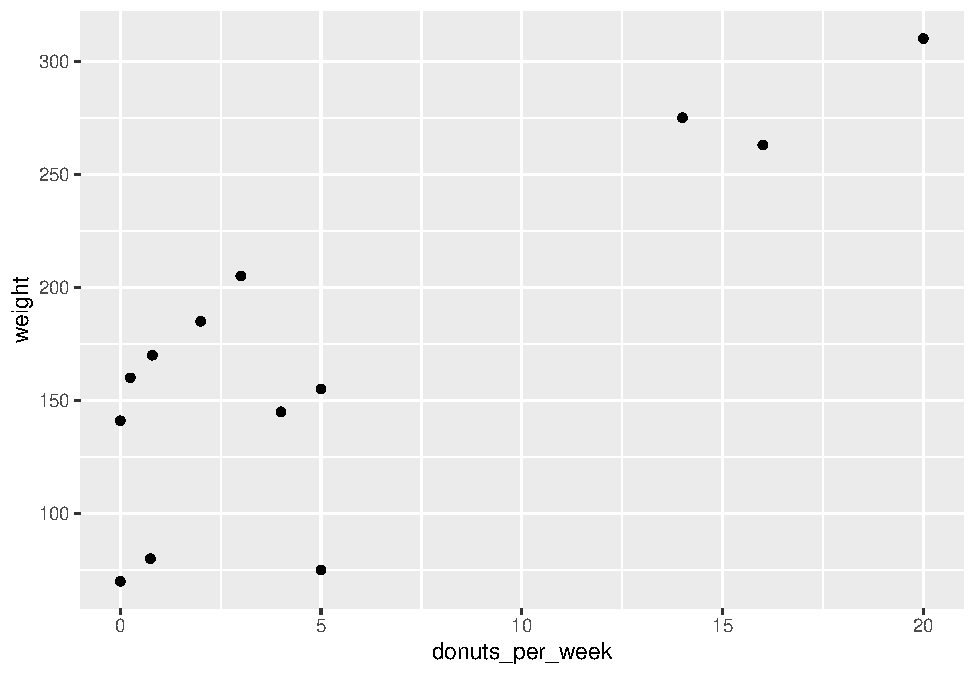
\includegraphics{bailey_files/figure-latex/figure1.2-1.pdf}

\begin{Shaded}
\begin{Highlighting}[]
\CommentTok{# the parentheses surrounding the function call cause the output to be printed.}
\end{Highlighting}
\end{Shaded}

This basic plot can be transformed into the figure in the text by adding layers to the graphic to change its appearance.

\begin{Shaded}
\begin{Highlighting}[]
\CommentTok{# Change the axis labels and add a caption}
\NormalTok{(p2 <-}\StringTok{ }\NormalTok{p1 }\OperatorTok{+}\StringTok{ }\KeywordTok{labs}\NormalTok{(}\DataTypeTok{x =} \StringTok{"Donuts"}\NormalTok{, }\DataTypeTok{y =} \StringTok{"Weight (in pounds)"}\NormalTok{, }\DataTypeTok{caption =} \StringTok{"Figure 1.2: Weight and Donuts in Springfield"}\NormalTok{)) }
\end{Highlighting}
\end{Shaded}

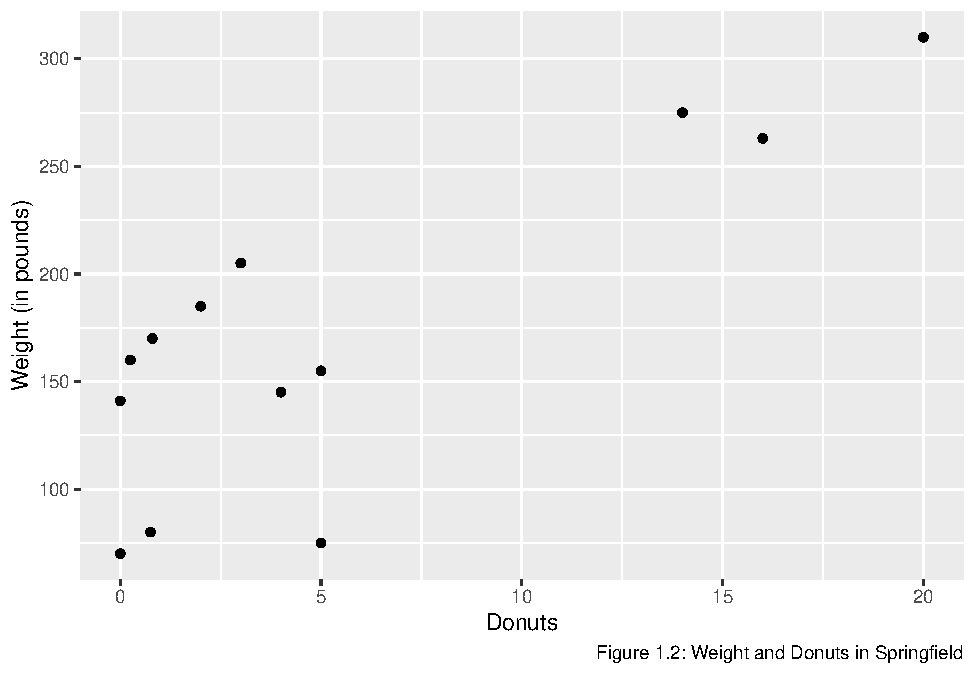
\includegraphics{bailey_files/figure-latex/unnamed-chunk-3-1.pdf}

\begin{Shaded}
\begin{Highlighting}[]
\CommentTok{# Add the verticle line at 0}
\NormalTok{(p3 <-}\StringTok{ }\NormalTok{p2 }\OperatorTok{+}\StringTok{ }\KeywordTok{geom_vline}\NormalTok{(}\DataTypeTok{xintercept =} \DecValTok{0}\NormalTok{, }\DataTypeTok{color =} \StringTok{"gray80"}\NormalTok{, }\DataTypeTok{size =} \FloatTok{1.25}\NormalTok{))}
\end{Highlighting}
\end{Shaded}

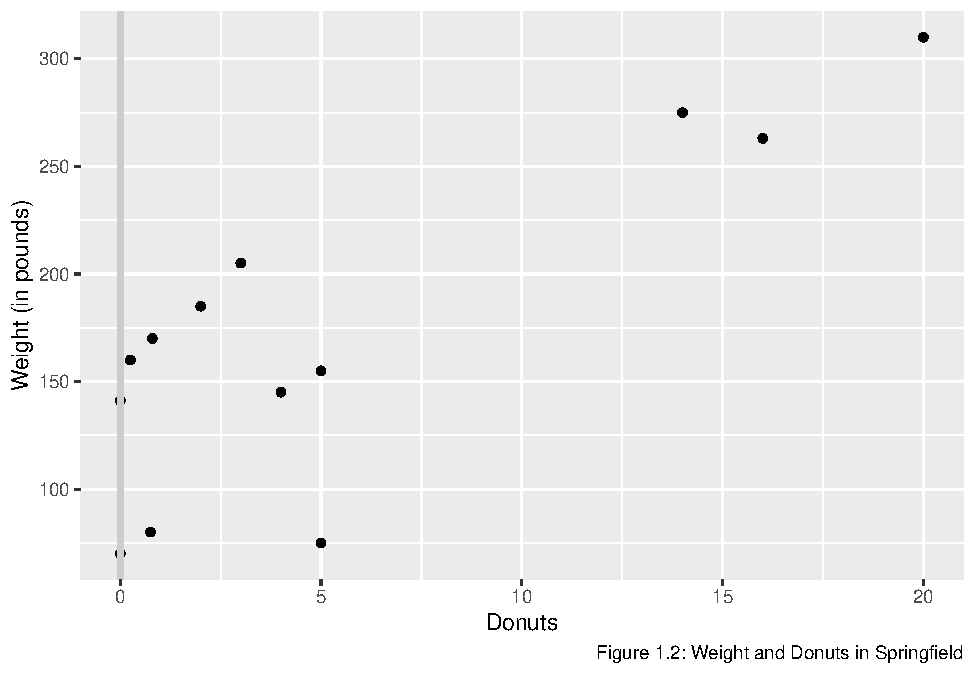
\includegraphics{bailey_files/figure-latex/unnamed-chunk-3-2.pdf}

\begin{Shaded}
\begin{Highlighting}[]
\CommentTok{# the layering effect puts the line in front of the points, so we have to add it before geom_point}
\NormalTok{(p4 <-}\StringTok{ }\NormalTok{p2 }\OperatorTok{+}\StringTok{ }\CommentTok{#indentation makes to code easier to audit}
\StringTok{    }\KeywordTok{geom_vline}\NormalTok{(}\DataTypeTok{xintercept =} \DecValTok{0}\NormalTok{, }\DataTypeTok{color =} \StringTok{"gray80"}\NormalTok{, }\DataTypeTok{size =} \DecValTok{1}\NormalTok{) }\OperatorTok{+}
\StringTok{    }\KeywordTok{geom_point}\NormalTok{())}
\end{Highlighting}
\end{Shaded}

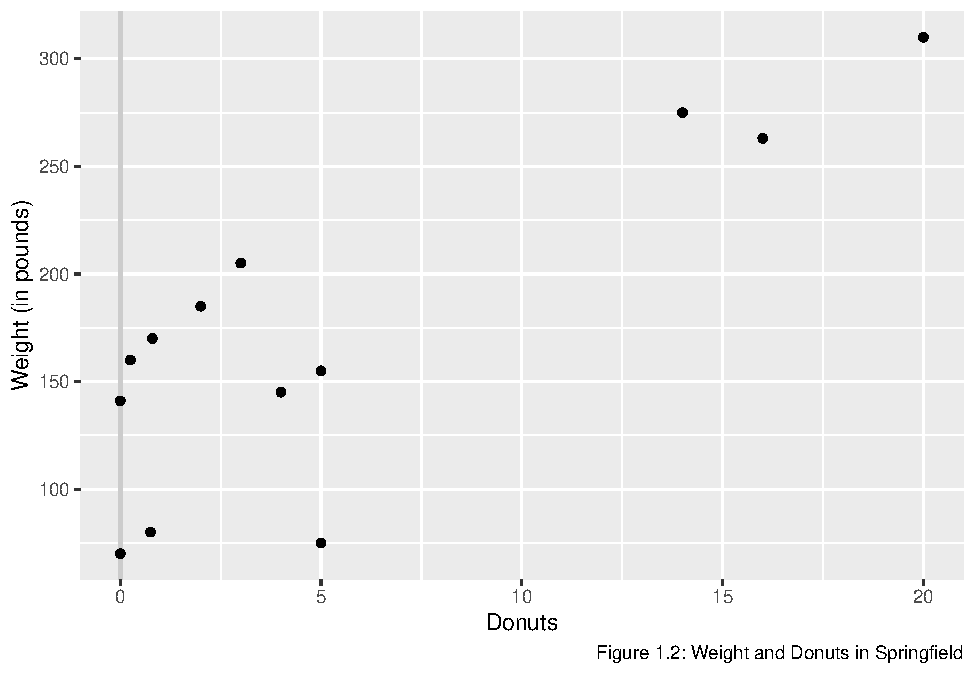
\includegraphics{bailey_files/figure-latex/unnamed-chunk-3-3.pdf}

\begin{Shaded}
\begin{Highlighting}[]
\CommentTok{# Add the name labels}
\NormalTok{(p5 <-}\StringTok{ }\NormalTok{p4 }\OperatorTok{+}\StringTok{ }\KeywordTok{geom_text}\NormalTok{(}\KeywordTok{aes}\NormalTok{(}\DataTypeTok{label =}\NormalTok{ name)))}
\end{Highlighting}
\end{Shaded}

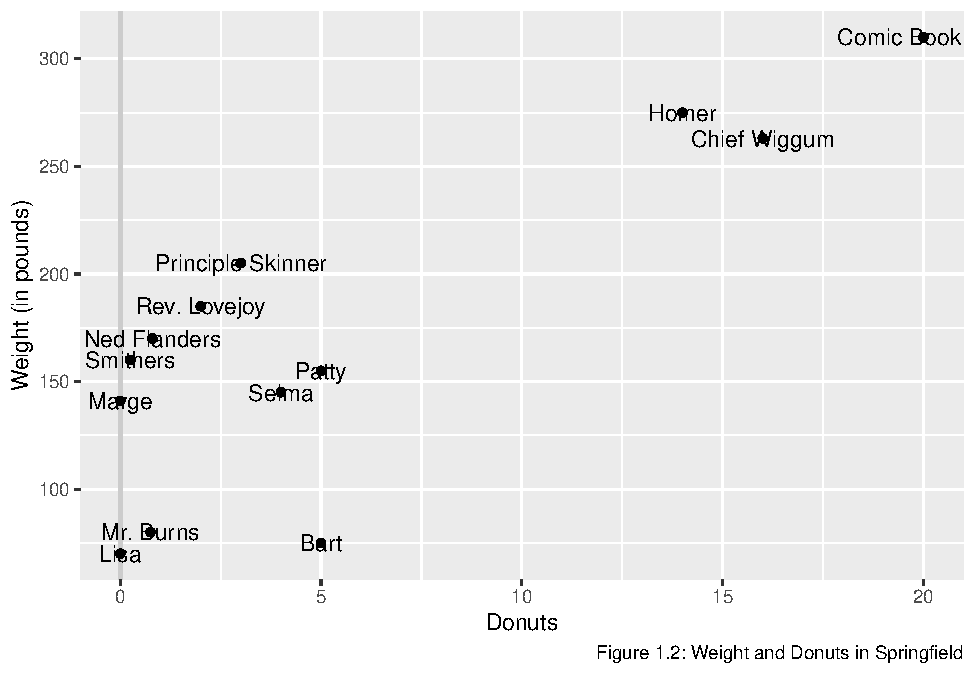
\includegraphics{bailey_files/figure-latex/unnamed-chunk-3-4.pdf}

\begin{Shaded}
\begin{Highlighting}[]
\CommentTok{# Clean up the name labels with the ggrepel package}
\KeywordTok{library}\NormalTok{(ggrepel)}
\NormalTok{(p6 <-}\StringTok{ }\NormalTok{p4 }\OperatorTok{+}\StringTok{ }\KeywordTok{geom_text_repel}\NormalTok{(}\KeywordTok{aes}\NormalTok{(}\DataTypeTok{label =}\NormalTok{ name)))}
\end{Highlighting}
\end{Shaded}

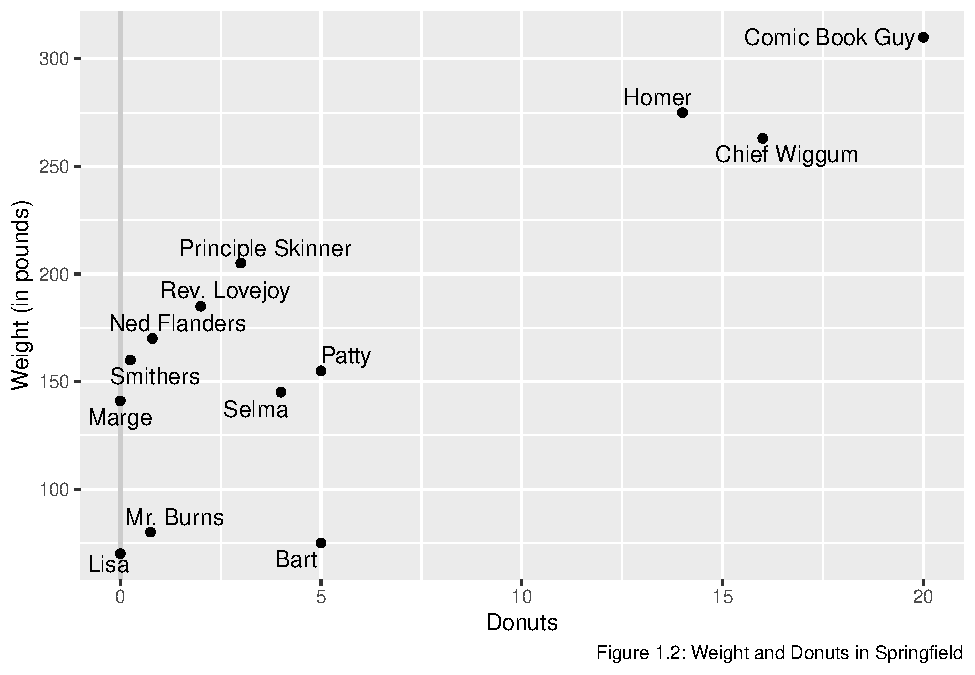
\includegraphics{bailey_files/figure-latex/unnamed-chunk-3-5.pdf}

\begin{Shaded}
\begin{Highlighting}[]
\CommentTok{# Use theme to adjust the non data elements}
\CommentTok{# \textbackslash{}n in the y label creates a new line}
\NormalTok{(p7 <-}\StringTok{ }\NormalTok{p6 }\OperatorTok{+}\StringTok{ }\KeywordTok{labs}\NormalTok{(}\DataTypeTok{y =} \StringTok{"Weight}\CharTok{\textbackslash{}n}\StringTok{(in pounds)"}\NormalTok{) }\OperatorTok{+}\StringTok{ }
\StringTok{    }\KeywordTok{theme}\NormalTok{(}\DataTypeTok{axis.title.y =} \KeywordTok{element_text}\NormalTok{(}\DataTypeTok{angle =} \DecValTok{0}\NormalTok{), }\CommentTok{# change orientation of y-axis label}
          \DataTypeTok{panel.grid =} \KeywordTok{element_blank}\NormalTok{(), }\CommentTok{# remove the background grid}
          \DataTypeTok{panel.background =} \KeywordTok{element_blank}\NormalTok{(), }\CommentTok{# remove the background}
          \DataTypeTok{axis.line =} \KeywordTok{element_line}\NormalTok{(), }\CommentTok{# add x and y axes}
          \DataTypeTok{plot.caption =} \KeywordTok{element_text}\NormalTok{(}\DataTypeTok{hjust =} \DecValTok{0}\NormalTok{))) }\CommentTok{#move the caption to the left.}
\end{Highlighting}
\end{Shaded}

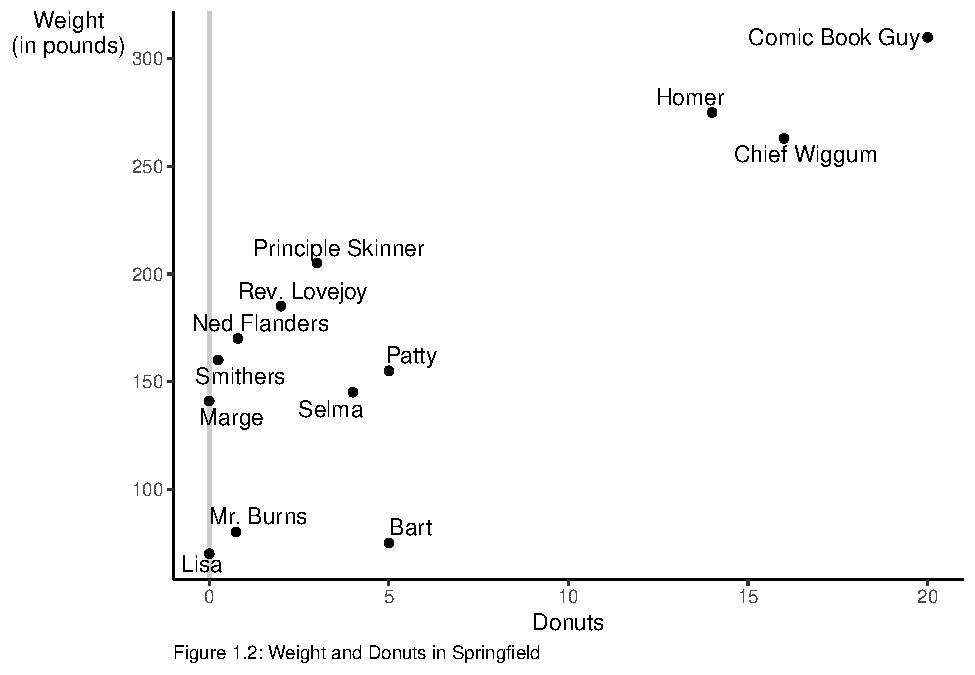
\includegraphics{bailey_files/figure-latex/unnamed-chunk-3-6.pdf}

We can make the graph in one step, if we desire.

\begin{Shaded}
\begin{Highlighting}[]
\NormalTok{p <-}\StringTok{ }\KeywordTok{ggplot}\NormalTok{(}\DataTypeTok{data =}\NormalTok{ donuts, }
       \DataTypeTok{mapping =} \KeywordTok{aes}\NormalTok{(}\DataTypeTok{x =}\NormalTok{ donuts_per_week, }\DataTypeTok{y =}\NormalTok{ weight)) }\OperatorTok{+}\StringTok{ }
\StringTok{  }\KeywordTok{geom_vline}\NormalTok{(}\DataTypeTok{xintercept =} \DecValTok{0}\NormalTok{, }\DataTypeTok{color =} \StringTok{"gray80"}\NormalTok{, }\DataTypeTok{size =} \DecValTok{1}\NormalTok{) }\OperatorTok{+}
\StringTok{  }\KeywordTok{geom_point}\NormalTok{() }\OperatorTok{+}\StringTok{ }
\StringTok{  }\KeywordTok{labs}\NormalTok{(}\DataTypeTok{x =} \StringTok{"Donuts"}\NormalTok{, }
       \DataTypeTok{y =} \StringTok{"Weight}\CharTok{\textbackslash{}n}\StringTok{(in pounds)"}\NormalTok{, }\CommentTok{# \textbackslash{}n creates a new line}
       \DataTypeTok{caption =} \StringTok{"Figure 1.2: Weight and Donuts in Springfield"}\NormalTok{) }\OperatorTok{+}\StringTok{ }
\StringTok{  }\KeywordTok{geom_text_repel}\NormalTok{(}\KeywordTok{aes}\NormalTok{(}\DataTypeTok{label =}\NormalTok{ name)) }\OperatorTok{+}
\StringTok{  }\KeywordTok{theme}\NormalTok{(}\DataTypeTok{axis.title.y =} \KeywordTok{element_text}\NormalTok{(}\DataTypeTok{angle =} \DecValTok{0}\NormalTok{), }
          \DataTypeTok{panel.grid =} \KeywordTok{element_blank}\NormalTok{(), }
          \DataTypeTok{panel.background =} \KeywordTok{element_blank}\NormalTok{(), }
          \DataTypeTok{axis.line =} \KeywordTok{element_line}\NormalTok{(), }
          \DataTypeTok{plot.caption =} \KeywordTok{element_text}\NormalTok{(}\DataTypeTok{hjust =} \DecValTok{0}\NormalTok{)) }
\NormalTok{p }
\end{Highlighting}
\end{Shaded}

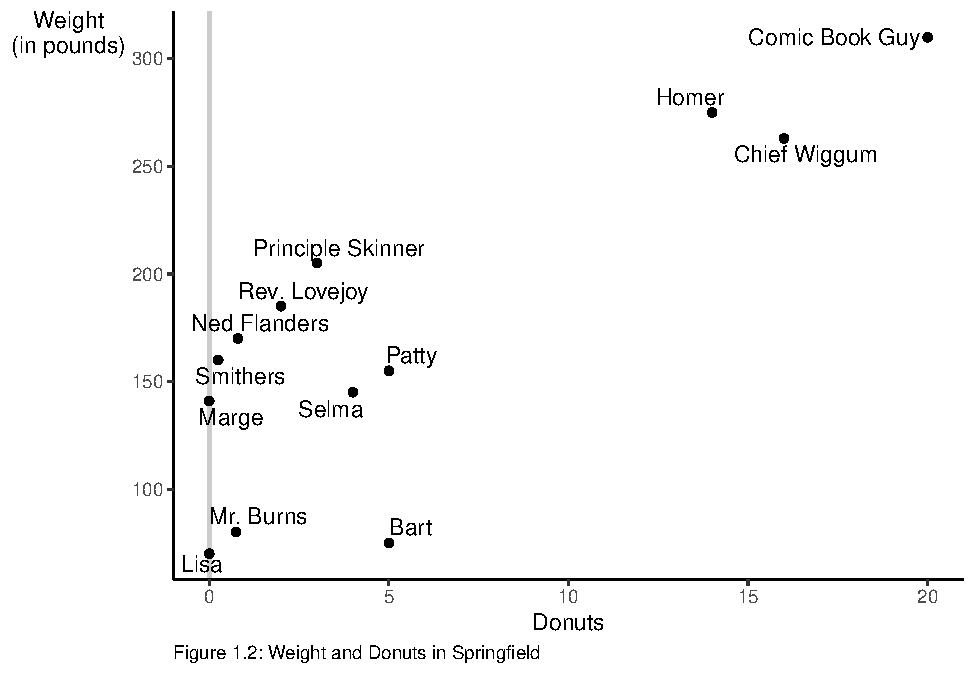
\includegraphics{bailey_files/figure-latex/figure1.2 again-1.pdf}

\hypertarget{figure-1.3}{%
\subsection{Figure 1.3}\label{figure-1.3}}

To create Figure 1.3, we start with the plot above we saved as an object, p.~We add an additional geometric, geom\_smooth to add the regression line.

\begin{Shaded}
\begin{Highlighting}[]
\NormalTok{p }\OperatorTok{+}\StringTok{ }\KeywordTok{labs}\NormalTok{(}\DataTypeTok{caption =} \StringTok{"Figure 1.3: Regression Line for Weight and Donuts in Springfield"}\NormalTok{) }\OperatorTok{+}\StringTok{ }
\StringTok{  }\KeywordTok{geom_smooth}\NormalTok{(}\DataTypeTok{method =} \StringTok{"lm"}\NormalTok{, }\DataTypeTok{se =}\NormalTok{ F) }\OperatorTok{+}\StringTok{ }\CommentTok{# method specifies the fit,  se = F turns off the error band.}
\StringTok{  }\KeywordTok{annotate}\NormalTok{(}\StringTok{"text"}\NormalTok{, }\DataTypeTok{label =} \KeywordTok{expression}\NormalTok{(beta[}\DecValTok{1}\NormalTok{]}\OperatorTok{*}\StringTok{" (the slope)"}\NormalTok{), }\CommentTok{# text annotation}
           \DataTypeTok{y =} \DecValTok{205}\NormalTok{, }\CommentTok{# position of the text}
           \DataTypeTok{x =} \DecValTok{8}\NormalTok{,   }\CommentTok{# position of the text}
           \DataTypeTok{angle =} \DecValTok{20}\NormalTok{, }\CommentTok{# angle of the text}
           \DataTypeTok{color =} \StringTok{"Blue"}\NormalTok{) }\OperatorTok{+}\StringTok{ }\CommentTok{# color of the text}
\StringTok{  }\KeywordTok{geom_segment}\NormalTok{(}\KeywordTok{aes}\NormalTok{(}\DataTypeTok{y =} \FloatTok{121.613}\NormalTok{, }\DataTypeTok{x =} \DecValTok{0}\NormalTok{, }\DataTypeTok{xend =} \DecValTok{0}\NormalTok{, }\DataTypeTok{yend =} \DecValTok{0}\NormalTok{),}
               \DataTypeTok{color =} \StringTok{"blue"}\NormalTok{,}
               \DataTypeTok{linetype =} \StringTok{"dotted"}\NormalTok{,}
               \DataTypeTok{size =} \DecValTok{1}\NormalTok{) }\OperatorTok{+}\StringTok{ }
\StringTok{  }\KeywordTok{annotate}\NormalTok{(}\StringTok{"text"}\NormalTok{, }\DataTypeTok{label =} \KeywordTok{expression}\NormalTok{(beta[}\DecValTok{0}\NormalTok{]}\OperatorTok{*}\StringTok{" = 121.613"}\NormalTok{),}
           \DataTypeTok{y =} \DecValTok{115}\NormalTok{, }\DataTypeTok{x =} \FloatTok{1.75}\NormalTok{, }\DataTypeTok{size =} \FloatTok{3.5}\NormalTok{, }\DataTypeTok{color =} \StringTok{"blue"}\NormalTok{)}
\end{Highlighting}
\end{Shaded}

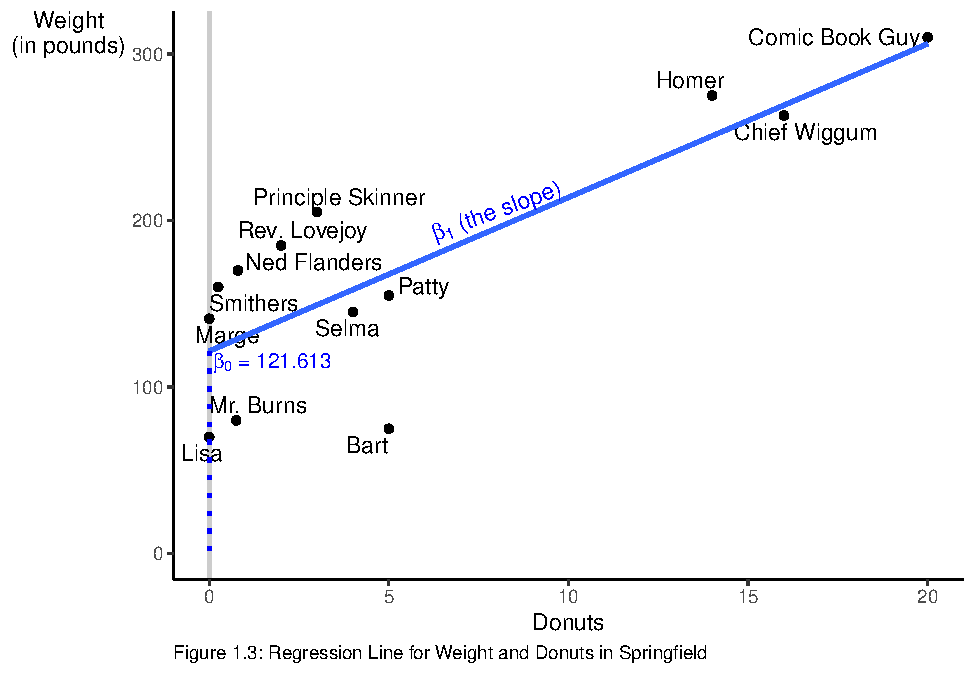
\includegraphics{bailey_files/figure-latex/figure1.3-1.pdf}

\hypertarget{chp2}{%
\chapter{Stats in the Wild: Good Data Practices}\label{chp2}}

\hypertarget{introduction-1}{%
\section{Introduction}\label{introduction-1}}

I will introduce some additional R commands and packages through reproducing Table 2.1, Table 2.2, Table 2.5, and Figure 2.3. In addition, we will go through the \emph{Computing Corner}.

\hypertarget{table-and-figure-reproduction}{%
\section{Table and Figure Reproduction}\label{table-and-figure-reproduction}}

\hypertarget{table-2.1}{%
\subsection{Table 2.1}\label{table-2.1}}

Since we saved the data frame we created in Chapter 1 as donuts.RData, we will \texttt{load} the file into global environment. We are only interested in the summary statistics for Weight and Donuts. We can get a basic set of summary statistics by calling \texttt{summary} on the data frame. But, \texttt{stargazer} from
the stargazer package. The stargazer produces well formatted tables in LaTex code, HTML code, and ASCII text.

We will make use of the pipe operator from the \texttt{magrittr} package (also part of the \texttt{tidyverse}), as well. The pipe operator \texttt{\%\textgreater{}\%} (ctr-shift-m shortcut in R Studio) allows for more intuitive reading of code especially when nesting commands inside of each other. Take a simple example of finding calling the \texttt{str} command on a data frame, \texttt{df}. Without the pipe operator \texttt{\%\textgreater{}\%}, we would call the command like this \texttt{str(df)} and you might read this aloud alike this find the structure of df. With the pipe operator, call the command like this \texttt{df\ \%\textgreater{}\%\ str()}. Read aloud it might be something like this ``take the \texttt{df} data and find its structure.'' The pipe operator really shines when functions are nested together, as we shall see below.

\begin{Shaded}
\begin{Highlighting}[]
\KeywordTok{load}\NormalTok{(}\StringTok{"donuts.RData"}\NormalTok{)}
\KeywordTok{library}\NormalTok{(tidyverse)}
\KeywordTok{library}\NormalTok{(stargazer)}
\NormalTok{donuts }\OperatorTok\StringTok{ }
\StringTok{  }\KeywordTok{select}\NormalTok{(}\StringTok{"Weight"}\NormalTok{ =}\StringTok{ }\NormalTok{weight, }\StringTok{"Donuts"}\NormalTok{ =}\StringTok{ }\NormalTok{donuts_per_week) }\OperatorTok\StringTok{ }\CommentTok{# choose and rename the columns}
\StringTok{  }\NormalTok{as.data.frame }\OperatorTok\StringTok{ }\CommentTok{# stargazer doesn't play nice with tibbles}
\StringTok{    }\KeywordTok{stargazer}\NormalTok{(}\DataTypeTok{type =} \StringTok{"text"}\NormalTok{, }\CommentTok{# tell stargazer to produce an ASCII text version of the table}
              \DataTypeTok{title =} \StringTok{"Table 2.1"}\NormalTok{, }
              \DataTypeTok{omit.summary.stat =} \KeywordTok{c}\NormalTok{(}\StringTok{"p25"}\NormalTok{, }\StringTok{"p75"}\NormalTok{)) }\CommentTok{# omit the default 1st and 3rd quartiles}
\end{Highlighting}
\end{Shaded}

\begin{verbatim}

Table 2.1
=====================================
Statistic N   Mean   St. Dev. Min Max
-------------------------------------
Weight    13 172.000  76.200  70  310
Donuts    13  5.450   6.750    0  20 
-------------------------------------
\end{verbatim}

\hypertarget{table-2.2}{%
\subsection{Table 2.2}\label{table-2.2}}

To reproduce Table 2.2 we will need to add a variable named male which will take on the value 1 for each observation in the data that represents a male and a 0 otherwise.

\begin{Shaded}
\begin{Highlighting}[]
\KeywordTok{load}\NormalTok{(}\StringTok{"donuts.RData"}\NormalTok{)}
\NormalTok{donuts}\OperatorTok{$}\NormalTok{name }\CommentTok{# this syntax reads print the variable name from the donuts data frame.}
\end{Highlighting}
\end{Shaded}

\begin{verbatim}
 [1] "Homer"             "Marge"             "Lisa"             
 [4] "Bart"              "Comic Book Guy"    "Mr. Burns"        
 [7] "Smithers"          "Chief Wiggum"      "Principle Skinner"
[10] "Rev. Lovejoy"      "Ned Flanders"      "Patty"            
[13] "Selma"            
\end{verbatim}

Making use of donuts\$name we see that the observations 1, 4, 5, 6, 7, 8, 9, 10, 11 are male and observations 2, 3, 12, 13 are not. We add the variable male to the donuts data frame as follows:

\begin{Shaded}
\begin{Highlighting}[]
\NormalTok{donuts}\OperatorTok{$}\NormalTok{male <-}\StringTok{ }\KeywordTok{c}\NormalTok{(}\DecValTok{1}\NormalTok{, }\DecValTok{0}\NormalTok{, }\DecValTok{0}\NormalTok{, }\DecValTok{1}\NormalTok{, }\DecValTok{1}\NormalTok{, }\DecValTok{1}\NormalTok{, }\DecValTok{1}\NormalTok{, }\DecValTok{1}\NormalTok{, }\DecValTok{1}\NormalTok{, }\DecValTok{1}\NormalTok{, }\DecValTok{1}\NormalTok{, }\DecValTok{0}\NormalTok{, }\DecValTok{0}\NormalTok{)}
\end{Highlighting}
\end{Shaded}

Call \texttt{table} to create a rudimentary version of Table 2.2

\begin{Shaded}
\begin{Highlighting}[]
\NormalTok{donuts}\OperatorTok{$}\NormalTok{male }\OperatorTok\StringTok{ }
\StringTok{  }\KeywordTok{table}\NormalTok{()}
\end{Highlighting}
\end{Shaded}

\begin{verbatim}
.
0 1 
4 9 
\end{verbatim}

\hypertarget{table-2.5}{%
\subsection{Table 2.5}\label{table-2.5}}

To reproduce Table 2.5 we must first retrieve the data. We will retrieve the data directly from the agencies responsible for their collection. You can retrieve the data as a comma-separated values (\texttt{csv}) file. A \texttt{csv} file is a plain text file in which the data are stored in a tabular format with values separated by a comma.

The crime data can be found on the U.S. Department of Justice Federal Bureau of Investigation Uniform Crime Reporting Statistics \href{https://www.ucrdatatool.gov/}{website}. The single parent, urban, and poverty data can found on the U.S. Census \href{https://www.census.gov/}{website}.

An investigation of the CrimeOneYearofData.csv file shows that there is meta information contained in the file along with the data. We could open the csv file in Excel and edited to remove the information or we could read it directly into R using \texttt{read\_csv} from the \texttt{readr} package with options to ignore the meta information. The readr package has many advantages over the base R read functions, see \texttt{vignette("readr")} for more information. All of the text's data files are available in \texttt{csv} format, so we will make repeated use of \texttt{read-csv}. Investigation of the file with either Excel or text editor, shows the first nine rows are either blank or contain information about the data. Rows 63 to 183 contain footnotes and other additional information about the data. The names of the variables are in row ten of the csv file; so, we will skip the first nine rows using the option \texttt{skip}. We can choose the rows that contain the states and Washington, D.C., with the \texttt{n\_max} option. Also, we need only the columns that contain the state names and the violent crime numbers. After reading in the data we will use \texttt{select} from the \texttt{dplyr} package.

Similar to \texttt{ggplot} being based on the grammar of graphics, \texttt{dplyr} is a grammar of data manipulation. dplyr consists of a set of ``verbs'' to help solve common data manipulation problems. To learn more about dplyr read \texttt{vignette("dplyr")}, visit \href{https://dplyr.tidyverse.org/}{dplyr}, or for a good introduction visit the \href{https://r4ds.had.co.nz/transform.html}{data import chapter} in \emph{R for Data Science}. We will make use of the pipe operator from the \texttt{magrittr} package (also part of the \texttt{tidyverse}), as well.

\begin{Shaded}
\begin{Highlighting}[]
\KeywordTok{library}\NormalTok{(readr)}
\NormalTok{crime_one_year_of_data <-}\StringTok{ }\KeywordTok{read_csv}\NormalTok{(}\StringTok{"Data/CrimeOneYearofData.csv"}\NormalTok{, }\CommentTok{# read the data from its location}
                               \DataTypeTok{skip =} \DecValTok{9}\NormalTok{, }\CommentTok{# start at row 10}
                               \DataTypeTok{n_max =} \DecValTok{51}\NormalTok{) }\OperatorTok\StringTok{ }\CommentTok{# use only 51 records (ignores the US total row)}
\StringTok{  }\KeywordTok{select}\NormalTok{(}\KeywordTok{c}\NormalTok{(}\DecValTok{1}\NormalTok{,}\DecValTok{3}\NormalTok{)) }\CommentTok{# select only the first and third columns}
\end{Highlighting}
\end{Shaded}

Using \texttt{glimpse} from dplyr, we see that we have a tibble with 51 observations and 2 variables. \texttt{glimpse} is similar to \texttt{str}.

\begin{Shaded}
\begin{Highlighting}[]
\NormalTok{crime_one_year_of_data }\OperatorTok\StringTok{ }
\StringTok{  }\NormalTok{glimpse}
\end{Highlighting}
\end{Shaded}

\begin{verbatim}
Observations: 51
Variables: 2
$ State                <chr> "Alabama", "Alaska", "Arizona", "Arkansas...
$ `Violent Crime rate` <dbl> 450, 633, 426, 516, 473, 339, 301, 645, 1...
\end{verbatim}

We can see that State is a character vector and Violent Crime Rate is a numeric vector. Looking at the names of the variables we can see they do not adhere to the stylistic guidelines discussed above. The State variable begins with a capital letter and the Violent Crime Variable has capital letters and spaces in its name (the spaces are why you see the tick mark ```'' before and after the name). The state names are spelled out, but to reproduce Figure 2.3 we need to change those to two-letter abbreviations.

To bring the names into stylistic guidelines we can use \texttt{clean\_names} from the janitor package, \texttt{snake\ case} is the default conversion. Note, the versatility of the \texttt{\%\textgreater{}\%} operator. If we did not use the \texttt{\%\textgreater{}\%} operator, the code would have been written as \texttt{glimpse(crime\_one\_year\_of\_data\ \textless{}-\ clean\_names(crime\_one\_year\_of\_data))}

\begin{Shaded}
\begin{Highlighting}[]
\KeywordTok{library}\NormalTok{(janitor)}
\NormalTok{crime_one_year_of_data <-}\StringTok{ }\NormalTok{crime_one_year_of_data }\OperatorTok\StringTok{ }
\StringTok{  }\KeywordTok{clean_names}\NormalTok{() }\OperatorTok\StringTok{ }
\StringTok{  }\NormalTok{glimpse}
\end{Highlighting}
\end{Shaded}

\begin{verbatim}
Observations: 51
Variables: 2
$ state              <chr> "Alabama", "Alaska", "Arizona", "Arkansas",...
$ violent_crime_rate <dbl> 450, 633, 426, 516, 473, 339, 301, 645, 134...
\end{verbatim}

We will read the other data in a similar fashion.

\begin{Shaded}
\begin{Highlighting}[]
\CommentTok{# Source: U.S. Census Bureau, 2009 American Community Survey, Table C23008}
\NormalTok{ACS_}\DecValTok{09}\NormalTok{_1YR_C23008_with_ann <-}\StringTok{ }\KeywordTok{read_csv}\NormalTok{(}\StringTok{"Data/ACS_09_1YR_C23008_with_ann.csv"}\NormalTok{, }
    \DataTypeTok{skip =} \DecValTok{1}\NormalTok{,}
    \DataTypeTok{n_max =} \DecValTok{51}\NormalTok{) }\OperatorTok\StringTok{ }
\StringTok{  }\KeywordTok{clean_names}\NormalTok{() }
\KeywordTok{names}\NormalTok{(ACS_}\DecValTok{09}\NormalTok{_1YR_C23008_with_ann)[}\KeywordTok{names}\NormalTok{(ACS_}\DecValTok{09}\NormalTok{_1YR_C23008_with_ann) }\OperatorTok{==}\StringTok{ "geography"}\NormalTok{] <-}\StringTok{ "state"}
\CommentTok{# names(ACS_09_1YR_C23008_with_ann) looks at all the names }
\CommentTok{# [names(ACS_09_1YR_C23008_with_ann) == "geography"] extracts the column number of the name we want to change}
\CommentTok{# <- "state" assigns the name state to that column number}
\NormalTok{ACS_}\DecValTok{09}\NormalTok{_1YR_C23008_with_ann }\OperatorTok\StringTok{ }\KeywordTok{glimpse}\NormalTok{()}
\end{Highlighting}
\end{Shaded}

\begin{verbatim}
Observations: 51
Variables: 8
$ id                                            <chr> "0400000US01", "...
$ id2                                           <chr> "01", "02", "04"...
$ state                                         <chr> "Alabama", "Alas...
$ estimate_total                                <dbl> 1059528, 174634,...
$ estimate_under_6_years                        <dbl> 357122, 61489, 5...
$ estimate_under_6_years_living_with_one_parent <dbl> 141977, 20676, 2...
$ estimate_6_to_17_years                        <dbl> 702406, 113145, ...
$ estimate_6_to_17_years_living_with_one_parent <dbl> 270077, 32250, 3...
\end{verbatim}

To create the percentage of children with single parents, add those under 6 living with one parent to those between 6 and 17 living with one parent and divide by the estimated total. We create the new variable with the \texttt{mutate} verb from dplyr and \texttt{select} state and percent with single parents into a new data frame.

\begin{Shaded}
\begin{Highlighting}[]
\NormalTok{single_parents <-}\StringTok{ }
\NormalTok{ACS_}\DecValTok{09}\NormalTok{_1YR_C23008_with_ann }\OperatorTok\StringTok{ }
\StringTok{  }\KeywordTok{mutate}\NormalTok{(}\DataTypeTok{percent_single_parents =} 
\NormalTok{           (estimate_under_}\DecValTok{6}\NormalTok{_years_living_with_one_parent }\OperatorTok{+}\StringTok{ }
\StringTok{              }\NormalTok{estimate_}\DecValTok{6}\NormalTok{_to_}\DecValTok{17}\NormalTok{_years_living_with_one_parent) }\OperatorTok{/}\StringTok{ }
\StringTok{           }\NormalTok{estimate_total) }\OperatorTok\StringTok{ }
\StringTok{  }\KeywordTok{select}\NormalTok{(state, percent_single_parents) }\OperatorTok\StringTok{ }
\StringTok{  }\KeywordTok{glimpse}\NormalTok{()}
\end{Highlighting}
\end{Shaded}

\begin{verbatim}
Observations: 51
Variables: 2
$ state                  <chr> "Alabama", "Alaska", "Arizona", "Arkans...
$ percent_single_parents <dbl> 0.389, 0.303, 0.365, 0.378, 0.324, 0.28...
\end{verbatim}

\begin{Shaded}
\begin{Highlighting}[]
\CommentTok{# Source: U.S. Census Bureau, 2009 American Community Survey, Table S1701}
\NormalTok{ACS_}\DecValTok{09}\NormalTok{_1YR_S1701_with_ann <-}\StringTok{ }\KeywordTok{read_csv}\NormalTok{(}\StringTok{"Data/ACS_09_1YR_S1701_with_ann.csv"}\NormalTok{, }
    \DataTypeTok{skip =} \DecValTok{1}\NormalTok{,}
    \DataTypeTok{n_max =} \DecValTok{51}\NormalTok{) }\OperatorTok\StringTok{ }
\StringTok{  }\KeywordTok{clean_names}\NormalTok{() }\OperatorTok\StringTok{ }
\StringTok{  }\KeywordTok{select}\NormalTok{(}\StringTok{"state"}\NormalTok{ =}\StringTok{ }\NormalTok{geography, }\CommentTok{# directly name the variables when selected}
         \StringTok{"percent_poverty"}\NormalTok{ =}\StringTok{ }\NormalTok{percent_below_poverty_level_estimate_population_for_whom_poverty_status_is_determined) }\OperatorTok\StringTok{ }
\StringTok{  }\KeywordTok{glimpse}\NormalTok{()}
\end{Highlighting}
\end{Shaded}

\begin{verbatim}
Observations: 51
Variables: 2
$ state           <chr> "Alabama", "Alaska", "Arizona", "Arkansas", "C...
$ percent_poverty <dbl> 17.5, 9.0, 16.5, 18.8, 14.2, 12.9, 9.4, 10.8, ...
\end{verbatim}

To create the percent urban in 2009, we need to interpolate using the 2000 and 2010 censuses. After reading each set of data we will combine them into one data frame using \texttt{right\_join} from the dplyr package.

\begin{Shaded}
\begin{Highlighting}[]
\CommentTok{# Source: U.S. Census Bureau, Table P002}
\NormalTok{DEC_}\DecValTok{00}\NormalTok{_SF1_P002_with_ann <-}\StringTok{ }\KeywordTok{read_csv}\NormalTok{(}\StringTok{"Data/DEC_00_SF1_P002_with_ann.csv"}\NormalTok{, }
    \DataTypeTok{skip =} \DecValTok{1}\NormalTok{) }\OperatorTok\StringTok{ }
\StringTok{  }\KeywordTok{clean_names}\NormalTok{() }\OperatorTok
\StringTok{  }\KeywordTok{select}\NormalTok{(}\StringTok{"state"}\NormalTok{ =}\StringTok{ }\NormalTok{geography, }\StringTok{"total_00"}\NormalTok{ =}\StringTok{ }\NormalTok{total , }\StringTok{"urban_00"}\NormalTok{ =}\StringTok{ }\NormalTok{urban) }\OperatorTok\StringTok{ }
\StringTok{  }\KeywordTok{glimpse}\NormalTok{()}
\end{Highlighting}
\end{Shaded}

\begin{verbatim}
Observations: 51
Variables: 3
$ state    <chr> "Alabama", "Alaska", "Arizona", "Arkansas", "Californ...
$ total_00 <dbl> 4447100, 626932, 5130632, 2673400, 33871648, 4301261,...
$ urban_00 <dbl> 2465673, 411257, 4523535, 1404179, 31989663, 3633185,...
\end{verbatim}

\begin{Shaded}
\begin{Highlighting}[]
\CommentTok{# Source: U.S. Census Bureau, Table H2}
\NormalTok{DEC_}\DecValTok{10}\NormalTok{_SF1_P2_with_ann <-}\StringTok{ }\KeywordTok{read_csv}\NormalTok{(}\StringTok{"Data/DEC_10_SF1_P2_with_ann.csv"}\NormalTok{, }
    \DataTypeTok{skip =} \DecValTok{1}\NormalTok{) }\OperatorTok\StringTok{ }
\StringTok{  }\KeywordTok{clean_names}\NormalTok{() }\OperatorTok
\StringTok{  }\KeywordTok{select}\NormalTok{(}\StringTok{"state"}\NormalTok{ =}\StringTok{ }\NormalTok{geography, }\StringTok{"total_10"}\NormalTok{ =}\StringTok{ }\NormalTok{total , }\StringTok{"urban_10"}\NormalTok{ =}\StringTok{ }\NormalTok{urban) }\OperatorTok\StringTok{ }
\StringTok{  }\KeywordTok{glimpse}\NormalTok{()}
\end{Highlighting}
\end{Shaded}

\begin{verbatim}
Observations: 51
Variables: 3
$ state    <chr> "Alabama", "Alaska", "Arizona", "Arkansas", "Californ...
$ total_10 <chr> "4779736(r38235)", "710231(r38823)", "6392017", "2915...
$ urban_10 <dbl> 2821804, 468893, 5740659, 1637589, 35373606, 4332761,...
\end{verbatim}

Note that total\_10 from the 2010 census is a character vector. This means that there is at least one observation that includes characters. In fact, we can see at least 3 of the observations include parenthetical notes. \texttt{print} the variable to the screen to confirm each of the patterns is of the form ``(some text)''.

\begin{Shaded}
\begin{Highlighting}[]
\NormalTok{DEC_}\DecValTok{10}\NormalTok{_SF1_P2_with_ann}\OperatorTok{$}\NormalTok{total_}\DecValTok{10}
\end{Highlighting}
\end{Shaded}

\begin{verbatim}
 [1] "4779736(r38235)"  "710231(r38823)"   "6392017"         
 [4] "2915918(r39193)"  "37253956"         "5029196"         
 [7] "3574097"          "897934"           "601723(r39494)"  
[10] "18801310(r40184)" "9687653(r41102)"  "1360301"         
[13] "1567582(r41542)"  "12830632"         "6483802"         
[16] "3046355"          "2853118"          "4339367"         
[19] "4533372"          "1328361"          "5773552(r42264)" 
[22] "6547629"          "9883640(r45127)"  "5303925"         
[25] "2967297"          "5988927"          "989415"          
[28] "1826341"          "2700551"          "1316470"         
[31] "8791894(r46246)"  "2059179(r46748)"  "19378102"        
[34] "9535483"          "672591"           "11536504"        
[37] "3751351"          "3831074"          "12702379"        
[40] "1052567"          "4625364"          "814180(r48166)"  
[43] "6346105"          "25145561(r48514)" "2763885"         
[46] "625741"           "8001024"          "6724540"         
[49] "1852994"          "5686986"          "563626"          
\end{verbatim}

We have confirmed that undesirable string has the same form in each position it exists. We must remove those comments and coerce the variable to numeric to proceed. We can determine how many instances of these comments occur using \texttt{str\_detect} from the \texttt{stringr} package. \texttt{str\_detect} will return a logical vector, so we need only sum the vector to count the number of times this occurs.

When calling \texttt{sum} on a logical vector, TRUE is treated as 1 and FALSE as 0, so summing the vector ``counts'' the number of TRUE occurrences. A regular expression, \texttt{regex} or \texttt{regexp}, is a sequence of characters that define a search pattern, to learn more visit \href{https://regexr.com/}{regexr.com}. The pattern we are looking for here is given by ``\textbackslash{}(.+\textbackslash{})''. Since the parenthesis is a special character, it must be escaped with \textbackslash{}, the . is a wild card, the + means 1 or more, so the .+ means find anything that appears 1 or more times. So the expression can be read as start with ( find anything which occurs one or more times and end with ).

\begin{Shaded}
\begin{Highlighting}[]
\KeywordTok{str_detect}\NormalTok{(DEC_}\DecValTok{10}\NormalTok{_SF1_P2_with_ann}\OperatorTok{$}\NormalTok{total_}\DecValTok{10}\NormalTok{, }\StringTok{"}\CharTok{\textbackslash{}\textbackslash{}}\StringTok{(.+}\CharTok{\textbackslash{}\textbackslash{}}\StringTok{)"}\NormalTok{) }\OperatorTok\StringTok{ }
\StringTok{  }\KeywordTok{sum}\NormalTok{()}
\end{Highlighting}
\end{Shaded}

\begin{verbatim}
[1] 13
\end{verbatim}

The pattern occurs 13 times. We need to remove the string and coerce the character vector to a numeric vector. \texttt{str\_replace\_all} will remove all occurrences of the string. \texttt{as.numeric} will coerce the character vector to a numeric vector. We will make use of the ``two-way'' pipe operator \texttt{\%\textless{}\textgreater{}\%} in each function call. This operator takes the left hand side passes it to to the function and returns the result back to the original vector effectively overwriting it.

\begin{Shaded}
\begin{Highlighting}[]
\KeywordTok{library}\NormalTok{(magrittr)}
\CommentTok{# the  %<>% operator is a "two way" pipe that sends the result back to the left hand side.}
\NormalTok{DEC_}\DecValTok{10}\NormalTok{_SF1_P2_with_ann}\OperatorTok{$}\NormalTok{total_}\DecValTok{10} \OperatorTok\StringTok{ }\KeywordTok{str_replace_all}\NormalTok{(}\StringTok{"}\CharTok{\textbackslash{}\textbackslash{}}\StringTok{(.+}\CharTok{\textbackslash{}\textbackslash{}}\StringTok{)"}\NormalTok{, }\StringTok{""}\NormalTok{) }\CommentTok{# "" replaces the string with blank}
\NormalTok{DEC_}\DecValTok{10}\NormalTok{_SF1_P2_with_ann}\OperatorTok{$}\NormalTok{total_}\DecValTok{10} \OperatorTok\StringTok{ }\KeywordTok{as.numeric}\NormalTok{()}
\NormalTok{DEC_}\DecValTok{10}\NormalTok{_SF1_P2_with_ann }\OperatorTok\StringTok{ }\KeywordTok{glimpse}\NormalTok{()}
\end{Highlighting}
\end{Shaded}

\begin{verbatim}
Observations: 51
Variables: 3
$ state    <chr> "Alabama", "Alaska", "Arizona", "Arkansas", "Californ...
$ total_10 <dbl> 4779736, 710231, 6392017, 2915918, 37253956, 5029196,...
$ urban_10 <dbl> 2821804, 468893, 5740659, 1637589, 35373606, 4332761,...
\end{verbatim}

We see that total\_10 is now a numeric vector.

We can now combine the two data frames using \texttt{right\_join} from the dplyr package. Since each data frame has the state variable, \texttt{right\_join} will add the columns from the 2010 census to the end (right) of the 2000 census matching observations by state. We will assign the result to percent\_urban.

\begin{Shaded}
\begin{Highlighting}[]
\NormalTok{urban <-}\StringTok{ }\NormalTok{DEC_}\DecValTok{00}\NormalTok{_SF1_P002_with_ann }\OperatorTok\StringTok{ }
\StringTok{  }\KeywordTok{right_join}\NormalTok{(DEC_}\DecValTok{10}\NormalTok{_SF1_P2_with_ann) }\OperatorTok\StringTok{ }
\StringTok{  }\KeywordTok{glimpse}\NormalTok{()}
\end{Highlighting}
\end{Shaded}

\begin{verbatim}
Observations: 51
Variables: 5
$ state    <chr> "Alabama", "Alaska", "Arizona", "Arkansas", "Californ...
$ total_00 <dbl> 4447100, 626932, 5130632, 2673400, 33871648, 4301261,...
$ urban_00 <dbl> 2465673, 411257, 4523535, 1404179, 31989663, 3633185,...
$ total_10 <dbl> 4779736, 710231, 6392017, 2915918, 37253956, 5029196,...
$ urban_10 <dbl> 2821804, 468893, 5740659, 1637589, 35373606, 4332761,...
\end{verbatim}

We can, now, interpolate the 2009 observations from the 2000 and 2010 observations. Since 2009 is nine tenths of the distance to 2010 from 2000, we will add 9/10 of the difference between the two observations to the 2000 observation.

\begin{Shaded}
\begin{Highlighting}[]
\NormalTok{urban }\OperatorTok\StringTok{ }
\StringTok{  }\KeywordTok{mutate}\NormalTok{(}\DataTypeTok{percent_urban =}\NormalTok{ (.}\DecValTok{9} \OperatorTok{*}\StringTok{ }\NormalTok{(urban_}\DecValTok{10} \OperatorTok{-}\StringTok{ }\NormalTok{urban_}\DecValTok{00}\NormalTok{) }\OperatorTok{+}\StringTok{ }\NormalTok{urban_}\DecValTok{00}\NormalTok{) }\OperatorTok{/}\StringTok{ }
\StringTok{           }\NormalTok{(.}\DecValTok{9} \OperatorTok{*}\StringTok{ }\NormalTok{(total_}\DecValTok{10} \OperatorTok{-}\StringTok{ }\NormalTok{total_}\DecValTok{00}\NormalTok{) }\OperatorTok{+}\StringTok{ }\NormalTok{total_}\DecValTok{00}\NormalTok{) }\OperatorTok{*}\StringTok{ }\DecValTok{100}\NormalTok{) }\OperatorTok\StringTok{ }
\StringTok{  }\KeywordTok{select}\NormalTok{(state, percent_urban)}
\end{Highlighting}
\end{Shaded}

We now have 4 data frames containing the information we need to create Table 2.5 and Figure 2.3. We will create a one data frame by joining the four data frames using the dplyr package.

\begin{Shaded}
\begin{Highlighting}[]
\NormalTok{crime_df <-}\StringTok{ }\NormalTok{crime_one_year_of_data }\OperatorTok\StringTok{ }
\StringTok{  }\KeywordTok{right_join}\NormalTok{(single_parents) }\OperatorTok\StringTok{ }
\StringTok{  }\KeywordTok{right_join}\NormalTok{(urban) }\OperatorTok\StringTok{ }
\StringTok{  }\KeywordTok{right_join}\NormalTok{(ACS_}\DecValTok{09}\NormalTok{_1YR_S1701_with_ann) }\OperatorTok\StringTok{ }
\StringTok{  }\KeywordTok{glimpse}\NormalTok{()}
\end{Highlighting}
\end{Shaded}

\begin{verbatim}
Observations: 51
Variables: 5
$ state                  <chr> "Alabama", "Alaska", "Arizona", "Arkans...
$ violent_crime_rate     <dbl> 450, 633, 426, 516, 473, 339, 301, 645,...
$ percent_single_parents <dbl> 0.389, 0.303, 0.365, 0.378, 0.324, 0.28...
$ percent_urban          <dbl> 58.7, 66.0, 89.7, 55.8, 94.9, 86.0, 88....
$ percent_poverty        <dbl> 17.5, 9.0, 16.5, 18.8, 14.2, 12.9, 9.4,...
\end{verbatim}

Figure 2.3 includes state abbreviations rather than state names. We will change the names into abbreviations with the help of a built in character vector. state.name is character vector of state names, excluding Washington DC, built into R. We can concatenate that vector with the character string ``District of Columbia'', sort the new character vector alphabetically, convert the names to abbreviations with \texttt{state2abbr} from the \texttt{openintro} package, and assign the result to the state vector in the crime\_one\_year\_of\_data data frame.

\begin{Shaded}
\begin{Highlighting}[]
\KeywordTok{library}\NormalTok{(openintro)}
\NormalTok{state_abb <-}\StringTok{ }\KeywordTok{c}\NormalTok{(state.name, }\StringTok{"District of Columbia"}\NormalTok{) }\OperatorTok\StringTok{ }
\StringTok{  }\KeywordTok{sort}\NormalTok{() }\OperatorTok\StringTok{ }
\StringTok{  }\KeywordTok{state2abbr}\NormalTok{()}
\NormalTok{crime_df}\OperatorTok{$}\NormalTok{state <-}\StringTok{ }\NormalTok{state_abb  }
\NormalTok{crime_df }\OperatorTok\StringTok{ }\NormalTok{glimpse}
\end{Highlighting}
\end{Shaded}

\begin{verbatim}
Observations: 51
Variables: 5
$ state                  <chr> "AL", "AK", "AZ", "AR", "CA", "CO", "CT...
$ violent_crime_rate     <dbl> 450, 633, 426, 516, 473, 339, 301, 645,...
$ percent_single_parents <dbl> 0.389, 0.303, 0.365, 0.378, 0.324, 0.28...
$ percent_urban          <dbl> 58.7, 66.0, 89.7, 55.8, 94.9, 86.0, 88....
$ percent_poverty        <dbl> 17.5, 9.0, 16.5, 18.8, 14.2, 12.9, 9.4,...
\end{verbatim}

We proceed as we did with Table 2.1 to reproduce Table 2.3.

\begin{Shaded}
\begin{Highlighting}[]
\NormalTok{crime_df }\OperatorTok\StringTok{ }
\StringTok{  }\KeywordTok{select}\NormalTok{(}\StringTok{"Violent crime rate (per 100,00 people)"}\NormalTok{ =}\StringTok{ }\NormalTok{violent_crime_rate,}
         \StringTok{"Percent single parents"}\NormalTok{ =}\StringTok{ }\NormalTok{percent_single_parents,}
         \StringTok{"Percent urban"}\NormalTok{ =}\StringTok{ }\NormalTok{percent_urban,}
         \StringTok{"Percent poverty"}\NormalTok{ =}\StringTok{ }\NormalTok{percent_poverty) }\OperatorTok
\StringTok{  }\KeywordTok{as.data.frame}\NormalTok{() }\OperatorTok\StringTok{ }
\StringTok{  }\KeywordTok{stargazer}\NormalTok{(}\DataTypeTok{type =} \StringTok{"text"}\NormalTok{, }
            \DataTypeTok{title =} \StringTok{"Table 2.3"}\NormalTok{,}
            \DataTypeTok{omit.summary.stat =} \KeywordTok{c}\NormalTok{(}\StringTok{"p25"}\NormalTok{, }\StringTok{"p75"}\NormalTok{)) }
\end{Highlighting}
\end{Shaded}

\begin{verbatim}

Table 2.3
============================================================================
Statistic                              N   Mean   St. Dev.   Min      Max   
----------------------------------------------------------------------------
Violent crime rate (per 100,00 people) 51 407.000 206.000  120.000 1,349.000
Percent single parents                 51  0.332   0.064    0.185    0.608  
Percent urban                          51 73.900   14.900  38.800   100.000 
Percent poverty                        51 13.900   3.110    8.500   21.900  
----------------------------------------------------------------------------
\end{verbatim}

\hypertarget{figure-2.3}{%
\subsection{Figure 2.3}\label{figure-2.3}}

We will use \texttt{ggplot} from the \texttt{ggplot2} package to reproduce Figure 2.3. We will use the \texttt{plot\_grd} from \texttt{cowplot} package to create a grid of the three individual plots after we create them individually.

\begin{Shaded}
\begin{Highlighting}[]
\NormalTok{plot_urban <-}\StringTok{ }
\StringTok{  }\NormalTok{crime_df }\OperatorTok\StringTok{ }
\StringTok{  }\KeywordTok{ggplot}\NormalTok{(}\KeywordTok{aes}\NormalTok{(}\DataTypeTok{x =}\NormalTok{ percent_urban, }\DataTypeTok{y =}\NormalTok{ violent_crime_rate)) }\OperatorTok{+}
\StringTok{  }\KeywordTok{labs}\NormalTok{(}\DataTypeTok{x =} \StringTok{"Percent urban}\CharTok{\textbackslash{}n}\StringTok{(0-to-100 scale)"}\NormalTok{, }\CommentTok{# \textbackslash{}n creates a new line}
       \DataTypeTok{y =} \StringTok{"Violent}\CharTok{\textbackslash{}n}\StringTok{crime}\CharTok{\textbackslash{}n}\StringTok{rate}\CharTok{\textbackslash{}n}\StringTok{(per}\CharTok{\textbackslash{}n}\StringTok{100,000}\CharTok{\textbackslash{}n}\StringTok{people)"}\NormalTok{) }\OperatorTok{+}
\StringTok{  }\KeywordTok{geom_text}\NormalTok{(}\KeywordTok{aes}\NormalTok{(}\DataTypeTok{label =}\NormalTok{ state), }\DataTypeTok{color =} \StringTok{"blue"}\NormalTok{) }\OperatorTok{+}
\StringTok{  }\KeywordTok{scale_y_continuous}\NormalTok{(}\DataTypeTok{breaks =} \KeywordTok{seq}\NormalTok{(}\DecValTok{200}\NormalTok{, }\DecValTok{1200}\NormalTok{, }\DecValTok{200}\NormalTok{)) }\OperatorTok{+}\StringTok{ }\CommentTok{# creates a sequence from 200 to 1200 by 200}
\StringTok{  }\KeywordTok{scale_x_continuous}\NormalTok{(}\DataTypeTok{breaks =} \KeywordTok{seq}\NormalTok{(}\DecValTok{40}\NormalTok{, }\DecValTok{100}\NormalTok{, }\DecValTok{10}\NormalTok{)) }\OperatorTok{+}\StringTok{ }\CommentTok{# creates a sequence from 40 to 100 by 10}
\StringTok{  }\KeywordTok{theme}\NormalTok{(}\DataTypeTok{axis.title.y =} \KeywordTok{element_text}\NormalTok{(}\DataTypeTok{angle =} \DecValTok{0}\NormalTok{), }
        \DataTypeTok{panel.grid =} \KeywordTok{element_blank}\NormalTok{(), }
        \DataTypeTok{panel.background =} \KeywordTok{element_blank}\NormalTok{(), }
        \DataTypeTok{axis.line =} \KeywordTok{element_line}\NormalTok{())}

\NormalTok{plot_single <-}\StringTok{ }
\StringTok{  }\NormalTok{crime_df }\OperatorTok\StringTok{ }
\StringTok{  }\KeywordTok{ggplot}\NormalTok{(}\KeywordTok{aes}\NormalTok{(}\DataTypeTok{x =}\NormalTok{ percent_single_parents, }\DataTypeTok{y =}\NormalTok{ violent_crime_rate)) }\OperatorTok{+}
\StringTok{  }\KeywordTok{labs}\NormalTok{(}\DataTypeTok{x =} \StringTok{"Percent single parent}\CharTok{\textbackslash{}n}\StringTok{(0-to-1 scale)"}\NormalTok{, }\CommentTok{# \textbackslash{}n creates a new line}
       \DataTypeTok{y =} \StringTok{""}\NormalTok{) }\OperatorTok{+}
\StringTok{  }\KeywordTok{geom_text}\NormalTok{(}\KeywordTok{aes}\NormalTok{(}\DataTypeTok{label =}\NormalTok{ state), }\DataTypeTok{color =} \StringTok{"blue"}\NormalTok{) }\OperatorTok{+}
\StringTok{  }\KeywordTok{scale_y_continuous}\NormalTok{(}\DataTypeTok{breaks =} \KeywordTok{seq}\NormalTok{(}\DecValTok{200}\NormalTok{, }\DecValTok{1200}\NormalTok{, }\DecValTok{200}\NormalTok{)) }\OperatorTok{+}
\StringTok{  }\KeywordTok{theme}\NormalTok{(}\DataTypeTok{axis.title.y =} \KeywordTok{element_text}\NormalTok{(}\DataTypeTok{angle =} \DecValTok{0}\NormalTok{), }
        \DataTypeTok{panel.grid =} \KeywordTok{element_blank}\NormalTok{(), }
        \DataTypeTok{panel.background =} \KeywordTok{element_blank}\NormalTok{(), }
        \DataTypeTok{axis.line =} \KeywordTok{element_line}\NormalTok{())}

\NormalTok{plot_poverty <-}\StringTok{ }
\StringTok{  }\NormalTok{crime_df }\OperatorTok\StringTok{ }
\StringTok{  }\KeywordTok{ggplot}\NormalTok{(}\KeywordTok{aes}\NormalTok{(}\DataTypeTok{x =}\NormalTok{ percent_poverty, }\DataTypeTok{y =}\NormalTok{ violent_crime_rate)) }\OperatorTok{+}
\StringTok{  }\KeywordTok{labs}\NormalTok{(}\DataTypeTok{x =} \StringTok{"Percent poverty}\CharTok{\textbackslash{}n}\StringTok{(0-to-100 scale)"}\NormalTok{, }\CommentTok{# \textbackslash{}n creates a new line}
       \DataTypeTok{y =} \StringTok{""}\NormalTok{) }\OperatorTok{+}
\StringTok{  }\KeywordTok{geom_text}\NormalTok{(}\KeywordTok{aes}\NormalTok{(}\DataTypeTok{label =}\NormalTok{ state), }\DataTypeTok{color =} \StringTok{"blue"}\NormalTok{) }\OperatorTok{+}
\StringTok{  }\KeywordTok{scale_y_continuous}\NormalTok{(}\DataTypeTok{breaks =} \KeywordTok{seq}\NormalTok{(}\DecValTok{200}\NormalTok{, }\DecValTok{1200}\NormalTok{, }\DecValTok{200}\NormalTok{)) }\OperatorTok{+}
\StringTok{  }\KeywordTok{scale_x_continuous}\NormalTok{(}\DataTypeTok{breaks =} \KeywordTok{seq}\NormalTok{(}\DecValTok{8}\NormalTok{, }\DecValTok{22}\NormalTok{, }\DecValTok{2}\NormalTok{)) }\OperatorTok{+}
\StringTok{  }\KeywordTok{theme}\NormalTok{(}\DataTypeTok{axis.title.y =} \KeywordTok{element_text}\NormalTok{(}\DataTypeTok{angle =} \DecValTok{0}\NormalTok{), }
        \DataTypeTok{panel.grid =} \KeywordTok{element_blank}\NormalTok{(), }
        \DataTypeTok{panel.background =} \KeywordTok{element_blank}\NormalTok{(), }
        \DataTypeTok{axis.line =} \KeywordTok{element_line}\NormalTok{())}

\KeywordTok{library}\NormalTok{(cowplot)}
\KeywordTok{plot_grid}\NormalTok{(plot_urban, plot_single, plot_poverty,  }\DataTypeTok{ncol =} \DecValTok{3}\NormalTok{)}
\end{Highlighting}
\end{Shaded}

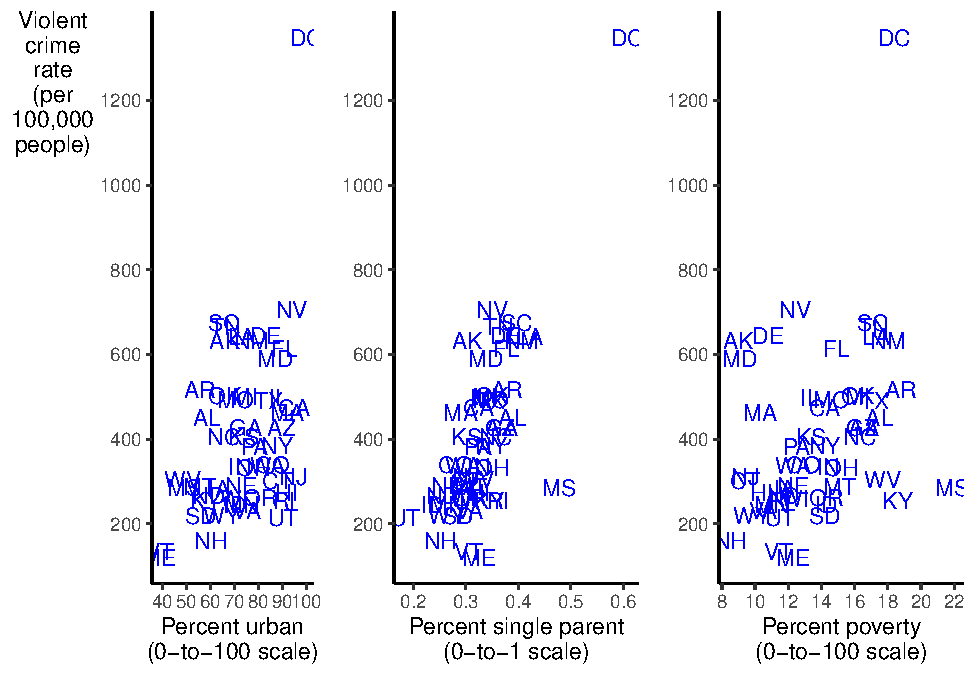
\includegraphics{bailey_files/figure-latex/unnamed-chunk-24-1.pdf}

FIGURE 2.3: Scatterplots of Violent Crime against Percent Urban, Single Parent, and Poverty

\hypertarget{computing-center}{%
\section{Computing Center}\label{computing-center}}

\hypertarget{reading-data}{%
\subsection{Reading Data}\label{reading-data}}

There are packages available to read data formatted in a variety of ways into R. Data can also be imported using the Import Dataset icon in the Environment/History pane. When learning to import data, this method can be useful as it will create the command line necessary to import the data, which you can then paste into your R Script of R Markdown file.

\hypertarget{manually-entering-data}{%
\subsection{Manually Entering Data}\label{manually-entering-data}}

In Chapter 1 we saw that we can directly (manually) enter data into R as well. Below is the appropriate syntax for doing so.

\begin{Shaded}
\begin{Highlighting}[]
\NormalTok{name <-}\StringTok{ }\KeywordTok{c}\NormalTok{(}\StringTok{"Homer"}\NormalTok{, }\StringTok{"Marge"}\NormalTok{, }\StringTok{"Lisa"}\NormalTok{, }\StringTok{"Bart"}\NormalTok{, }\StringTok{"Comic Book Guy"}\NormalTok{, }\StringTok{"Mr. Burns"}\NormalTok{, }\StringTok{"Smithers"}\NormalTok{, }\StringTok{"Chief Wiggum"}\NormalTok{, }\StringTok{"Principle Skinner"}\NormalTok{, }\StringTok{"Rev. Lovejoy"}\NormalTok{, }\StringTok{"Ned Flanders"}\NormalTok{, }\StringTok{"Patty"}\NormalTok{, }\StringTok{"Selma"}\NormalTok{)}
\NormalTok{donuts_per_week <-}\StringTok{ }\KeywordTok{c}\NormalTok{(}\DecValTok{14}\NormalTok{, }\DecValTok{0}\NormalTok{, }\DecValTok{0}\NormalTok{, }\DecValTok{5}\NormalTok{, }\DecValTok{20}\NormalTok{, }\FloatTok{0.75}\NormalTok{, }\FloatTok{0.25}\NormalTok{, }\DecValTok{16}\NormalTok{, }\DecValTok{3}\NormalTok{, }\DecValTok{2}\NormalTok{, }\FloatTok{0.8}\NormalTok{, }\DecValTok{5}\NormalTok{, }\DecValTok{4}\NormalTok{)}
\NormalTok{weight <-}\StringTok{ }\KeywordTok{c}\NormalTok{(}\DecValTok{275}\NormalTok{, }\DecValTok{141}\NormalTok{, }\DecValTok{70}\NormalTok{, }\DecValTok{75}\NormalTok{, }\DecValTok{310}\NormalTok{, }\DecValTok{80}\NormalTok{, }\DecValTok{160}\NormalTok{, }\DecValTok{263}\NormalTok{, }\DecValTok{205}\NormalTok{, }\DecValTok{185}\NormalTok{, }\DecValTok{170}\NormalTok{, }\DecValTok{155}\NormalTok{, }\DecValTok{145}\NormalTok{)}
\end{Highlighting}
\end{Shaded}

We can combine this into a single ``file'' called a data frame as follows:

\begin{Shaded}
\begin{Highlighting}[]
\NormalTok{Donuts <-}\StringTok{ }\KeywordTok{data.frame}\NormalTok{(name, donuts_per_week, weight)}
\NormalTok{Donuts }\OperatorTok\StringTok{ }
\StringTok{  }\KeywordTok{str}\NormalTok{()}
\end{Highlighting}
\end{Shaded}

\begin{verbatim}
'data.frame':   13 obs. of  3 variables:
 $ name           : Factor w/ 13 levels "Bart","Chief Wiggum",..: 4 6 5 1 3 7 13 2 10 11 ...
 $ donuts_per_week: num  14 0 0 5 20 0.75 0.25 16 3 2 ...
 $ weight         : num  275 141 70 75 310 80 160 263 205 185 ...
\end{verbatim}

The character vector ``name'' is coerced to a Factor by default. Factors in R are store as a vector of integer values with a corresponding set of character values. We will see that Factors are very useful, however, in this case we want name to remain a character vector. If we add the option \texttt{stringsAsFactors\ =\ FALSE} to our call of \texttt{data.frame} we can prevent the coercion. Our we can call \texttt{tibble} as described in Chapter 1.

\begin{Shaded}
\begin{Highlighting}[]
\NormalTok{Donuts <-}\StringTok{ }\KeywordTok{data.frame}\NormalTok{(name, donuts_per_week, weight, }\DataTypeTok{stringsAsFactors =} \OtherTok{FALSE}\NormalTok{)}
\NormalTok{Donuts }\OperatorTok\StringTok{ }\KeywordTok{str}\NormalTok{()}
\end{Highlighting}
\end{Shaded}

\begin{verbatim}
'data.frame':   13 obs. of  3 variables:
 $ name           : chr  "Homer" "Marge" "Lisa" "Bart" ...
 $ donuts_per_week: num  14 0 0 5 20 0.75 0.25 16 3 2 ...
 $ weight         : num  275 141 70 75 310 80 160 263 205 185 ...
\end{verbatim}

You can see in the Global Environment tab of the Environment/History pane that you have an object named Donuts that has 13 observations on 3 variables. In addition, you can see under values you have each variable as well.

\hypertarget{simple-statistics}{%
\subsection{Simple Statistics}\label{simple-statistics}}

R has many built in calls to get basic statistics on data. For example, to get the mean of a variable call \texttt{mean()}. Be aware, that if there are missing values in the data the function call will return NA as it's result. The donuts data frame contains to missing values ``NA'', so it won't be a problem. Some simple exploratory data analysis will let you know if you have any issues in the data. We saw one of those problems above when we had a variable that we thought was numeric, but was read in as a character vector. \texttt{summary} is a good place to start.

\begin{Shaded}
\begin{Highlighting}[]
\NormalTok{donuts }\OperatorTok\StringTok{ }
\StringTok{  }\KeywordTok{summary}\NormalTok{()}
\end{Highlighting}
\end{Shaded}

\begin{verbatim}
 observation_number     name           donuts_per_week     weight   
 Min.   : 1         Length:13          Min.   : 0.00   Min.   : 70  
 1st Qu.: 4         Class :character   1st Qu.: 0.75   1st Qu.:141  
 Median : 7         Mode  :character   Median : 3.00   Median :160  
 Mean   : 7                            Mean   : 5.45   Mean   :172  
 3rd Qu.:10                            3rd Qu.: 5.00   3rd Qu.:205  
 Max.   :13                            Max.   :20.00   Max.   :310  
      male      
 Min.   :0.000  
 1st Qu.:0.000  
 Median :1.000  
 Mean   :0.692  
 3rd Qu.:1.000  
 Max.   :1.000  
\end{verbatim}

We confirmed that there are no missing values in our data. If there were, we can easily deal with them with a option in the function call (I include the option below.)

\begin{Shaded}
\begin{Highlighting}[]
\NormalTok{donuts}\OperatorTok{$}\NormalTok{weight }\OperatorTok\StringTok{ }
\StringTok{  }\KeywordTok{mean}\NormalTok{(}\DataTypeTok{na.rm =} \OtherTok{TRUE}\NormalTok{)  }
\end{Highlighting}
\end{Shaded}

\begin{verbatim}
[1] 172
\end{verbatim}

Call \texttt{var} or \texttt{sd} to return the sample variance or sample standard deviation. Of course the standard deviation can also be calculated by calling \texttt{sqrt} on the result of the \texttt{var} call. There are multiple ways to retrieve the number of observations of a variable or data frame. The minimum and maximum values are returned by calling \texttt{min} and \texttt{max}. As described in the text, we can call \texttt{sum} on the result of the call \texttt{is.finite}. \texttt{nrow} will return the number of observations in a data frame, \texttt{NROW} will return the number of observations of a vector or single variable.

\begin{Shaded}
\begin{Highlighting}[]
\NormalTok{donuts}\OperatorTok{$}\NormalTok{weight }\OperatorTok\StringTok{ }\KeywordTok{var}\NormalTok{()}
\end{Highlighting}
\end{Shaded}

\begin{verbatim}
[1] 5800
\end{verbatim}

\begin{Shaded}
\begin{Highlighting}[]
\NormalTok{donuts}\OperatorTok{$}\NormalTok{weight }\OperatorTok\StringTok{ }\KeywordTok{var}\NormalTok{() }\OperatorTok\StringTok{ }\KeywordTok{sqrt}\NormalTok{()}
\end{Highlighting}
\end{Shaded}

\begin{verbatim}
[1] 76.2
\end{verbatim}

\begin{Shaded}
\begin{Highlighting}[]
\NormalTok{donuts}\OperatorTok{$}\NormalTok{weight }\OperatorTok\StringTok{ }\KeywordTok{sd}\NormalTok{()}
\end{Highlighting}
\end{Shaded}

\begin{verbatim}
[1] 76.2
\end{verbatim}

\begin{Shaded}
\begin{Highlighting}[]
\NormalTok{donuts}\OperatorTok{$}\NormalTok{weight }\OperatorTok\StringTok{ }\KeywordTok{min}\NormalTok{()}
\end{Highlighting}
\end{Shaded}

\begin{verbatim}
[1] 70
\end{verbatim}

\begin{Shaded}
\begin{Highlighting}[]
\NormalTok{donuts}\OperatorTok{$}\NormalTok{weight }\OperatorTok\StringTok{ }\KeywordTok{max}\NormalTok{()}
\end{Highlighting}
\end{Shaded}

\begin{verbatim}
[1] 310
\end{verbatim}

\begin{Shaded}
\begin{Highlighting}[]
\NormalTok{donuts}\OperatorTok{$}\NormalTok{weight }\OperatorTok\StringTok{ }\KeywordTok{NROW}\NormalTok{()}
\end{Highlighting}
\end{Shaded}

\begin{verbatim}
[1] 13
\end{verbatim}

To return a variety of descriptive statistics on a data frame or variable we can call \texttt{stargazer} from the stargazer package.

\begin{Shaded}
\begin{Highlighting}[]
\NormalTok{donuts }\OperatorTok\StringTok{ }
\StringTok{  }\NormalTok{as.data.frame }\OperatorTok\StringTok{ }
\StringTok{  }\KeywordTok{stargazer}\NormalTok{(}\DataTypeTok{type =} \StringTok{"text"}\NormalTok{)}
\end{Highlighting}
\end{Shaded}

\begin{verbatim}

================================================================
Statistic          N   Mean   St. Dev. Min Pctl(25) Pctl(75) Max
----------------------------------------------------------------
observation_number 13  7.000   3.890    1     4        10    13 
donuts_per_week    13  5.450   6.750    0    0.8       5     20 
weight             13 172.000  76.200  70    141      205    310
male               13  0.692   0.480    0     0        1      1 
----------------------------------------------------------------
\end{verbatim}

Subsetting in R can be accomplished in a variety of ways. In Base R, use {[}{]} syntax. Use brackets can be used to call specific rows and columns from a matrix or data frame. To return the observation in the 12\textsuperscript{th} row and 3rd column call \texttt{donuts{[}12,3{]}}. To return all of the observations in a specific row or column, leave the row or column number out of the call. To return all of the observations from the 3rd column call \texttt{donuts{[},3{]}}. To return the observations for an individual record, say the 4\textsuperscript{th} row, call \texttt{donuts{[}4,{]}}. To choose (subset) all of those records where, e.g,, donuts eaten per week is 0, call \texttt{donuts{[}donuts\$donuts\_per\_week\ ==\ 0,{]}}; to choose all those records where donuts donuts are not equal to 0, call \texttt{donuts{[}donuts\$donuts\_per\_week\ !=\ 0,{]}}. We can also subset using \texttt{filter} from \texttt{dplyr}. An advantage of subsetting with \texttt{dplyr} is that the resulting tibble can be piped into the another function call.

\begin{Shaded}
\begin{Highlighting}[]
\NormalTok{donuts[}\DecValTok{12}\NormalTok{,}\DecValTok{3}\NormalTok{]}
\end{Highlighting}
\end{Shaded}

\begin{verbatim}
# A tibble: 1 x 1
  donuts_per_week
            <dbl>
1               5
\end{verbatim}

\begin{Shaded}
\begin{Highlighting}[]
\NormalTok{donuts[,}\DecValTok{3}\NormalTok{]}
\end{Highlighting}
\end{Shaded}

\begin{verbatim}
# A tibble: 13 x 1
   donuts_per_week
             <dbl>
 1           14   
 2            0   
 3            0   
 4            5   
 5           20   
 6            0.75
 7            0.25
 8           16   
 9            3   
10            2   
11            0.8 
12            5   
13            4   
\end{verbatim}

\begin{Shaded}
\begin{Highlighting}[]
\NormalTok{donuts[}\DecValTok{4}\NormalTok{,]}
\end{Highlighting}
\end{Shaded}

\begin{verbatim}
# A tibble: 1 x 5
  observation_number name  donuts_per_week weight  male
               <int> <chr>           <dbl>  <dbl> <dbl>
1                  4 Bart                5     75     1
\end{verbatim}

\begin{Shaded}
\begin{Highlighting}[]
\NormalTok{donuts[donuts}\OperatorTok{$}\NormalTok{donuts_per_week }\OperatorTok{==}\StringTok{ }\DecValTok{0}\NormalTok{,]}
\end{Highlighting}
\end{Shaded}

\begin{verbatim}
# A tibble: 2 x 5
  observation_number name  donuts_per_week weight  male
               <int> <chr>           <dbl>  <dbl> <dbl>
1                  2 Marge               0    141     0
2                  3 Lisa                0     70     0
\end{verbatim}

\begin{Shaded}
\begin{Highlighting}[]
\NormalTok{donuts[donuts}\OperatorTok{$}\NormalTok{donuts_per_week }\OperatorTok{!=}\StringTok{ }\DecValTok{0}\NormalTok{,]}
\end{Highlighting}
\end{Shaded}

\begin{verbatim}
# A tibble: 11 x 5
   observation_number name              donuts_per_week weight  male
                <int> <chr>                       <dbl>  <dbl> <dbl>
 1                  1 Homer                       14       275     1
 2                  4 Bart                         5        75     1
 3                  5 Comic Book Guy              20       310     1
 4                  6 Mr. Burns                    0.75     80     1
 5                  7 Smithers                     0.25    160     1
 6                  8 Chief Wiggum                16       263     1
 7                  9 Principle Skinner            3       205     1
 8                 10 Rev. Lovejoy                 2       185     1
 9                 11 Ned Flanders                 0.8     170     1
10                 12 Patty                        5       155     0
11                 13 Selma                        4       145     0
\end{verbatim}

\begin{Shaded}
\begin{Highlighting}[]
\NormalTok{donuts }\OperatorTok\StringTok{ }
\StringTok{  }\KeywordTok{filter}\NormalTok{(donuts_per_week }\OperatorTok{==}\StringTok{ }\DecValTok{0}\NormalTok{)}
\end{Highlighting}
\end{Shaded}

\begin{verbatim}
# A tibble: 2 x 5
  observation_number name  donuts_per_week weight  male
               <int> <chr>           <dbl>  <dbl> <dbl>
1                  2 Marge               0    141     0
2                  3 Lisa                0     70     0
\end{verbatim}

\begin{Shaded}
\begin{Highlighting}[]
\NormalTok{donuts }\OperatorTok\StringTok{ }
\StringTok{  }\KeywordTok{filter}\NormalTok{(donuts_per_week }\OperatorTok{!=}\StringTok{ }\DecValTok{0}\NormalTok{)}
\end{Highlighting}
\end{Shaded}

\begin{verbatim}
# A tibble: 11 x 5
   observation_number name              donuts_per_week weight  male
                <int> <chr>                       <dbl>  <dbl> <dbl>
 1                  1 Homer                       14       275     1
 2                  4 Bart                         5        75     1
 3                  5 Comic Book Guy              20       310     1
 4                  6 Mr. Burns                    0.75     80     1
 5                  7 Smithers                     0.25    160     1
 6                  8 Chief Wiggum                16       263     1
 7                  9 Principle Skinner            3       205     1
 8                 10 Rev. Lovejoy                 2       185     1
 9                 11 Ned Flanders                 0.8     170     1
10                 12 Patty                        5       155     0
11                 13 Selma                        4       145     0
\end{verbatim}

We can subset on more than one variable as well. Using Base R we can choose all those males who consumed some donuts per week by calling \texttt{donuts{[}donuts\$donuts\_per\_week\ !=\ 0\ \&\ donuts\$male\ ==\ 1{]}}. We can choose all those observations where donut consumption per week is more than 15 or the person is female by using the or operator \textbar{} in call \texttt{donuts{[}donuts\$donuts\_per\_week\ \textgreater{}\ 15\ \textbar{}\ donuts\$male\ !=\ 1,{]}}. \texttt{filter} can be used as well.

\begin{Shaded}
\begin{Highlighting}[]
\NormalTok{donuts[donuts}\OperatorTok{$}\NormalTok{donuts_per_week }\OperatorTok{!=}\StringTok{ }\DecValTok{0} \OperatorTok{&}\StringTok{ }\NormalTok{donuts}\OperatorTok{$}\NormalTok{male }\OperatorTok{==}\StringTok{ }\DecValTok{1}\NormalTok{,]}
\end{Highlighting}
\end{Shaded}

\begin{verbatim}
# A tibble: 9 x 5
  observation_number name              donuts_per_week weight  male
               <int> <chr>                       <dbl>  <dbl> <dbl>
1                  1 Homer                       14       275     1
2                  4 Bart                         5        75     1
3                  5 Comic Book Guy              20       310     1
4                  6 Mr. Burns                    0.75     80     1
5                  7 Smithers                     0.25    160     1
6                  8 Chief Wiggum                16       263     1
7                  9 Principle Skinner            3       205     1
8                 10 Rev. Lovejoy                 2       185     1
9                 11 Ned Flanders                 0.8     170     1
\end{verbatim}

\begin{Shaded}
\begin{Highlighting}[]
\NormalTok{donuts }\OperatorTok\StringTok{ }
\StringTok{  }\KeywordTok{filter}\NormalTok{(donuts_per_week }\OperatorTok{!=}\StringTok{ }\DecValTok{0} \OperatorTok{&}\StringTok{ }\NormalTok{male }\OperatorTok{==}\StringTok{ }\DecValTok{1}\NormalTok{)}
\end{Highlighting}
\end{Shaded}

\begin{verbatim}
# A tibble: 9 x 5
  observation_number name              donuts_per_week weight  male
               <int> <chr>                       <dbl>  <dbl> <dbl>
1                  1 Homer                       14       275     1
2                  4 Bart                         5        75     1
3                  5 Comic Book Guy              20       310     1
4                  6 Mr. Burns                    0.75     80     1
5                  7 Smithers                     0.25    160     1
6                  8 Chief Wiggum                16       263     1
7                  9 Principle Skinner            3       205     1
8                 10 Rev. Lovejoy                 2       185     1
9                 11 Ned Flanders                 0.8     170     1
\end{verbatim}

\begin{Shaded}
\begin{Highlighting}[]
\CommentTok{# a slightly more intuitive alternative is:}
\NormalTok{donuts }\OperatorTok\StringTok{ }
\StringTok{  }\KeywordTok{filter}\NormalTok{(donuts_per_week }\OperatorTok{!=}\StringTok{ }\DecValTok{0}\NormalTok{) }\OperatorTok\StringTok{ }
\StringTok{  }\KeywordTok{filter}\NormalTok{(male }\OperatorTok{==}\StringTok{ }\DecValTok{1}\NormalTok{)  }
\end{Highlighting}
\end{Shaded}

\begin{verbatim}
# A tibble: 9 x 5
  observation_number name              donuts_per_week weight  male
               <int> <chr>                       <dbl>  <dbl> <dbl>
1                  1 Homer                       14       275     1
2                  4 Bart                         5        75     1
3                  5 Comic Book Guy              20       310     1
4                  6 Mr. Burns                    0.75     80     1
5                  7 Smithers                     0.25    160     1
6                  8 Chief Wiggum                16       263     1
7                  9 Principle Skinner            3       205     1
8                 10 Rev. Lovejoy                 2       185     1
9                 11 Ned Flanders                 0.8     170     1
\end{verbatim}

\begin{Shaded}
\begin{Highlighting}[]
\NormalTok{donuts[donuts}\OperatorTok{$}\NormalTok{donuts_per_week }\OperatorTok{>}\StringTok{ }\DecValTok{15} \OperatorTok{|}\StringTok{ }\NormalTok{donuts}\OperatorTok{$}\NormalTok{male }\OperatorTok{!=}\StringTok{ }\DecValTok{1}\NormalTok{,]}
\end{Highlighting}
\end{Shaded}

\begin{verbatim}
# A tibble: 6 x 5
  observation_number name           donuts_per_week weight  male
               <int> <chr>                    <dbl>  <dbl> <dbl>
1                  2 Marge                        0    141     0
2                  3 Lisa                         0     70     0
3                  5 Comic Book Guy              20    310     1
4                  8 Chief Wiggum                16    263     1
5                 12 Patty                        5    155     0
6                 13 Selma                        4    145     0
\end{verbatim}

\begin{Shaded}
\begin{Highlighting}[]
\NormalTok{donuts }\OperatorTok\StringTok{ }
\StringTok{  }\KeywordTok{filter}\NormalTok{(donuts_per_week }\OperatorTok{>}\StringTok{ }\DecValTok{15} \OperatorTok{|}\StringTok{ }\NormalTok{male }\OperatorTok{!=}\StringTok{ }\DecValTok{1}\NormalTok{)}
\end{Highlighting}
\end{Shaded}

\begin{verbatim}
# A tibble: 6 x 5
  observation_number name           donuts_per_week weight  male
               <int> <chr>                    <dbl>  <dbl> <dbl>
1                  2 Marge                        0    141     0
2                  3 Lisa                         0     70     0
3                  5 Comic Book Guy              20    310     1
4                  8 Chief Wiggum                16    263     1
5                 12 Patty                        5    155     0
6                 13 Selma                        4    145     0
\end{verbatim}

We can modify Figure 2.2 to include only males by modifying our original code by piping the filtered results into \texttt{ggplot}.

\begin{Shaded}
\begin{Highlighting}[]
\KeywordTok{library}\NormalTok{(ggrepel)}
\NormalTok{donuts }\OperatorTok\StringTok{ }
\StringTok{  }\KeywordTok{filter}\NormalTok{(male }\OperatorTok{==}\StringTok{ }\DecValTok{1}\NormalTok{) }\OperatorTok\StringTok{ }
\StringTok{  }\KeywordTok{ggplot}\NormalTok{(}\DataTypeTok{mapping =} \KeywordTok{aes}\NormalTok{(}\DataTypeTok{x =}\NormalTok{ donuts_per_week, }\DataTypeTok{y =}\NormalTok{ weight)) }\OperatorTok{+}\StringTok{ }
\StringTok{  }\KeywordTok{geom_vline}\NormalTok{(}\DataTypeTok{xintercept =} \DecValTok{0}\NormalTok{, }\DataTypeTok{color =} \StringTok{"gray80"}\NormalTok{, }\DataTypeTok{size =} \DecValTok{1}\NormalTok{) }\OperatorTok{+}
\StringTok{  }\KeywordTok{geom_point}\NormalTok{(}\DataTypeTok{color =} \StringTok{"blue"}\NormalTok{, }\DataTypeTok{size =} \DecValTok{2}\NormalTok{) }\OperatorTok{+}\StringTok{ }
\StringTok{  }\KeywordTok{labs}\NormalTok{(}\DataTypeTok{x =} \StringTok{"Donuts"}\NormalTok{, }
       \DataTypeTok{y =} \StringTok{"Weight}\CharTok{\textbackslash{}n}\StringTok{(in pounds)"}\NormalTok{, }\CommentTok{# \textbackslash{}n creates a new line}
       \DataTypeTok{caption =} \StringTok{"Figure 2.2: Weight and Donuts in Springfield"}\NormalTok{) }\OperatorTok{+}\StringTok{ }
\StringTok{  }\KeywordTok{geom_text_repel}\NormalTok{(}\KeywordTok{aes}\NormalTok{(}\DataTypeTok{label =}\NormalTok{ name), }\DataTypeTok{color =} \StringTok{"blue"}\NormalTok{) }\OperatorTok{+}
\StringTok{  }\KeywordTok{theme}\NormalTok{(}\DataTypeTok{axis.title.y =} \KeywordTok{element_text}\NormalTok{(}\DataTypeTok{angle =} \DecValTok{0}\NormalTok{), }
          \DataTypeTok{panel.grid =} \KeywordTok{element_blank}\NormalTok{(), }
          \DataTypeTok{panel.background =} \KeywordTok{element_blank}\NormalTok{(), }
          \DataTypeTok{axis.line =} \KeywordTok{element_line}\NormalTok{(), }
          \DataTypeTok{plot.caption =} \KeywordTok{element_text}\NormalTok{(}\DataTypeTok{hjust =} \DecValTok{0}\NormalTok{)) }
\end{Highlighting}
\end{Shaded}

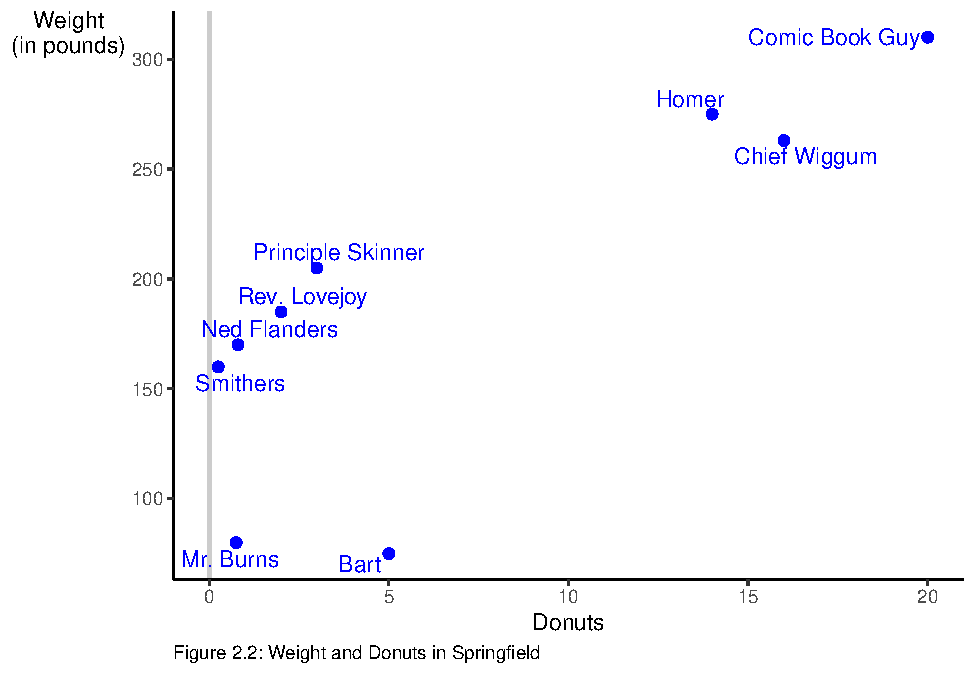
\includegraphics{bailey_files/figure-latex/figure2.2mod-1.pdf}

\hypertarget{cph3}{%
\chapter{Bivariate OLS: The Foundation of Econometric Analysis}\label{cph3}}

We will work through \emph{Computing Corner}.

\hypertarget{estimating-a-simple-regression}{%
\section{Estimating a simple regression}\label{estimating-a-simple-regression}}

To run a simple regression in R, make us of the function \texttt{lm}. Like all functions \texttt{lm} requires and argument list. You can see the arguments required and the defaualt values, if any, in a variety of ways in R Studio. \texttt{args(lm)} will return the arguments for the lm function. \texttt{?lm} will open the help page in the Files/Plots/Packages/Help Pane, which can also be accessed by typing lm in the search in the same pane. Estimating a regression using \texttt{lm} requires only two arguments: the formula and data arguments. If you provide those arguments in that order, R doesn't require that you use the argument's name. This is true for all functions in R, the default is that the arguments appear in order. We can see by calling \texttt{str} on ols\_donuts that \texttt{lm} creates a list object which contains 12 elements. A list is an object that contains elements of several different types like, strings, vectors, matrices, lists, etc. Each of those elements can be extracted from the list in much the same way as accessing pieces of a data frame.

\begin{Shaded}
\begin{Highlighting}[]
\KeywordTok{library}\NormalTok{(magrittr)}
\KeywordTok{load}\NormalTok{(}\StringTok{"donuts.RData"}\NormalTok{)}
\NormalTok{ols_donuts <-}\StringTok{ }\KeywordTok{lm}\NormalTok{(}\DataTypeTok{formula =}\NormalTok{ weight }\OperatorTok{~}\StringTok{ }\NormalTok{donuts_per_week, }\DataTypeTok{data =}\NormalTok{ donuts)}
\NormalTok{ols_donuts }\OperatorTok\StringTok{ }
\StringTok{  }\KeywordTok{str}\NormalTok{()}
\end{Highlighting}
\end{Shaded}

\begin{verbatim}
List of 12
 $ coefficients : Named num [1:2] 121.61 9.22
  ..- attr(*, "names")= chr [1:2] "(Intercept)" "donuts_per_week"
 $ residuals    : Named num [1:13] 24.26 19.39 -51.61 -92.73 3.92 ...
  ..- attr(*, "names")= chr [1:13] "1" "2" "3" "4" ...
 $ effects      : Named num [1:13] -619.6 215.66 -60.24 -99.06 4.49 ...
  ..- attr(*, "names")= chr [1:13] "(Intercept)" "donuts_per_week" "" "" ...
 $ rank         : int 2
 $ fitted.values: Named num [1:13] 251 122 122 168 306 ...
  ..- attr(*, "names")= chr [1:13] "1" "2" "3" "4" ...
 $ assign       : int [1:2] 0 1
 $ qr           :List of 5
  ..$ qr   : num [1:13, 1:2] -3.606 0.277 0.277 0.277 0.277 ...
  .. ..- attr(*, "dimnames")=List of 2
  .. .. ..$ : chr [1:13] "1" "2" "3" "4" ...
  .. .. ..$ : chr [1:2] "(Intercept)" "donuts_per_week"
  .. ..- attr(*, "assign")= int [1:2] 0 1
  ..$ qraux: num [1:2] 1.28 1.31
  ..$ pivot: int [1:2] 1 2
  ..$ tol  : num 0.0000001
  ..$ rank : int 2
  ..- attr(*, "class")= chr "qr"
 $ df.residual  : int 11
 $ xlevels      : Named list()
 $ call         : language lm(formula = weight ~ donuts_per_week, data = donuts)
 $ terms        :Classes 'terms', 'formula'  language weight ~ donuts_per_week
  .. ..- attr(*, "variables")= language list(weight, donuts_per_week)
  .. ..- attr(*, "factors")= int [1:2, 1] 0 1
  .. .. ..- attr(*, "dimnames")=List of 2
  .. .. .. ..$ : chr [1:2] "weight" "donuts_per_week"
  .. .. .. ..$ : chr "donuts_per_week"
  .. ..- attr(*, "term.labels")= chr "donuts_per_week"
  .. ..- attr(*, "order")= int 1
  .. ..- attr(*, "intercept")= int 1
  .. ..- attr(*, "response")= int 1
  .. ..- attr(*, ".Environment")=<environment: R_GlobalEnv> 
  .. ..- attr(*, "predvars")= language list(weight, donuts_per_week)
  .. ..- attr(*, "dataClasses")= Named chr [1:2] "numeric" "numeric"
  .. .. ..- attr(*, "names")= chr [1:2] "weight" "donuts_per_week"
 $ model        :'data.frame':  13 obs. of  2 variables:
  ..$ weight         : num [1:13] 275 141 70 75 310 80 160 263 205 185 ...
  ..$ donuts_per_week: num [1:13] 14 0 0 5 20 0.75 0.25 16 3 2 ...
  ..- attr(*, "terms")=Classes 'terms', 'formula'  language weight ~ donuts_per_week
  .. .. ..- attr(*, "variables")= language list(weight, donuts_per_week)
  .. .. ..- attr(*, "factors")= int [1:2, 1] 0 1
  .. .. .. ..- attr(*, "dimnames")=List of 2
  .. .. .. .. ..$ : chr [1:2] "weight" "donuts_per_week"
  .. .. .. .. ..$ : chr "donuts_per_week"
  .. .. ..- attr(*, "term.labels")= chr "donuts_per_week"
  .. .. ..- attr(*, "order")= int 1
  .. .. ..- attr(*, "intercept")= int 1
  .. .. ..- attr(*, "response")= int 1
  .. .. ..- attr(*, ".Environment")=<environment: R_GlobalEnv> 
  .. .. ..- attr(*, "predvars")= language list(weight, donuts_per_week)
  .. .. ..- attr(*, "dataClasses")= Named chr [1:2] "numeric" "numeric"
  .. .. .. ..- attr(*, "names")= chr [1:2] "weight" "donuts_per_week"
 - attr(*, "class")= chr "lm"
\end{verbatim}

You can see the type for each of the 12 elements in the list. Each of those elements can be extracted by using the \$ convention you use to get variables from a data frame (which is a type of list) as describe in the text. In addition, there are many commands that will extract a standard set of elements and present them in conventional ways. For example, to get the regression results, \texttt{summary} from base R, \texttt{stargazer} from the stargazer package, and \texttt{tidy} and \texttt{glance} from the \texttt{broom} package provide the output in useful ways. \texttt{augment} from the broom package creates a tibble of actual, fitted, residuals, etc. In fact, all of the commands in the \texttt{broom} package create tibbles which can useful for further analysis. \texttt{stargazer} can be modified to include a variety of statistics. So, you can extract fitted values or residuals, e.g., in the same way you retrieve any data from a data frame or tibble.

\begin{Shaded}
\begin{Highlighting}[]
\KeywordTok{library}\NormalTok{(tidyverse)}
\KeywordTok{library}\NormalTok{(broom)}
\KeywordTok{library}\NormalTok{(stargazer)}
\NormalTok{ols_donuts }\OperatorTok\StringTok{ }
\StringTok{  }\KeywordTok{summary}\NormalTok{()}
\end{Highlighting}
\end{Shaded}

\begin{verbatim}

Call:
lm(formula = weight ~ donuts_per_week, data = donuts)

Residuals:
   Min     1Q Median     3Q    Max 
-92.73 -13.51   3.92  36.08  55.72 

Coefficients:
                Estimate Std. Error t value Pr(>|t|)    
(Intercept)       121.61      16.59    7.33 0.000015 ***
donuts_per_week     9.22       1.96    4.71  0.00064 ***
---
Signif. codes:  0 '***' 0.001 '**' 0.01 '*' 0.05 '.' 0.1 ' ' 1

Residual standard error: 45.8 on 11 degrees of freedom
Multiple R-squared:  0.668, Adjusted R-squared:  0.638 
F-statistic: 22.2 on 1 and 11 DF,  p-value: 0.000643
\end{verbatim}

\begin{Shaded}
\begin{Highlighting}[]
\NormalTok{ols_donuts }\OperatorTok\StringTok{ }
\StringTok{  }\KeywordTok{stargazer}\NormalTok{(}\DataTypeTok{type =} \StringTok{"text"}\NormalTok{)}
\end{Highlighting}
\end{Shaded}

\begin{verbatim}

===============================================
                        Dependent variable:    
                    ---------------------------
                              weight           
-----------------------------------------------
donuts_per_week              9.220***          
                              (1.960)          
                                               
Constant                    122.000***         
                             (16.600)          
                                               
-----------------------------------------------
Observations                    13             
R2                             0.668           
Adjusted R2                    0.638           
Residual Std. Error      45.800 (df = 11)      
F Statistic           22.200*** (df = 1; 11)   
===============================================
Note:               *p<0.1; **p<0.05; ***p<0.01
\end{verbatim}

\begin{Shaded}
\begin{Highlighting}[]
\NormalTok{ols_donuts }\OperatorTok\StringTok{ }
\StringTok{  }\KeywordTok{tidy}\NormalTok{()}
\end{Highlighting}
\end{Shaded}

\begin{verbatim}
# A tibble: 2 x 5
  term            estimate std.error statistic   p.value
  <chr>              <dbl>     <dbl>     <dbl>     <dbl>
1 (Intercept)       122.       16.6       7.33 0.0000149
2 donuts_per_week     9.22      1.96      4.71 0.000643 
\end{verbatim}

\begin{Shaded}
\begin{Highlighting}[]
\NormalTok{ols_donuts }\OperatorTok\StringTok{ }
\StringTok{  }\KeywordTok{glance}\NormalTok{()}
\end{Highlighting}
\end{Shaded}

\begin{verbatim}
# A tibble: 1 x 11
  r.squared adj.r.squared sigma statistic p.value    df logLik   AIC   BIC
      <dbl>         <dbl> <dbl>     <dbl>   <dbl> <int>  <dbl> <dbl> <dbl>
1     0.668         0.638  45.8      22.2 6.43e-4     2  -67.1  140.  142.
# ... with 2 more variables: deviance <dbl>, df.residual <int>
\end{verbatim}

\begin{Shaded}
\begin{Highlighting}[]
\NormalTok{ols_donuts }\OperatorTok\StringTok{ }
\StringTok{  }\KeywordTok{augment}\NormalTok{()}
\end{Highlighting}
\end{Shaded}

\begin{verbatim}
# A tibble: 13 x 9
   weight donuts_per_week .fitted .se.fit .resid   .hat .sigma .cooksd
    <dbl>           <dbl>   <dbl>   <dbl>  <dbl>  <dbl>  <dbl>   <dbl>
 1    275           14       251.    21.0  24.3  0.211    47.3 0.0474 
 2    141            0       122.    16.6  19.4  0.131    47.6 0.0156 
 3     70            0       122.    16.6 -51.6  0.131    44.7 0.110  
 4     75            5       168.    12.7 -92.7  0.0773   37.1 0.186  
 5    310           20       306.    31.2   3.92 0.464    48.0 0.00591
 6     80            0.75    129.    15.7 -48.5  0.117    45.2 0.0844 
 7    160            0.25    124.    16.3  36.1  0.126    46.5 0.0513 
 8    263           16       269.    24.3  -6.19 0.281    48.0 0.00495
 9    205            3       149.    13.6  55.7  0.0879   44.4 0.0781 
10    185            2       140.    14.4  44.9  0.0986   45.7 0.0584 
11    170            0.8     129.    15.6  41.0  0.116    46.0 0.0597 
12    155            5       168.    12.7 -12.7  0.0773   47.9 0.00350
13    145            4       159.    13.0 -13.5  0.0807   47.8 0.00415
# ... with 1 more variable: .std.resid <dbl>
\end{verbatim}

\hypertarget{scatter-plot-with-regression-line}{%
\section{scatter Plot with Regression Line}\label{scatter-plot-with-regression-line}}

ggplot2 makes adding a fitted regression line to a scatter plot very easy. You need only add a geometry called geom\_smooth with the appropriate method to plot. The default is to include a confidence interval estimate around the fitted line. To remove the error band add the option \texttt{se\ =\ FALSE}.

\begin{Shaded}
\begin{Highlighting}[]
\NormalTok{donuts }\OperatorTok
\StringTok{  }\KeywordTok{ggplot}\NormalTok{(}\KeywordTok{aes}\NormalTok{(}\DataTypeTok{x =}\NormalTok{ donuts_per_week, }\DataTypeTok{y =}\NormalTok{ weight)) }\OperatorTok{+}
\StringTok{  }\KeywordTok{geom_point}\NormalTok{() }\OperatorTok{+}
\StringTok{  }\KeywordTok{geom_smooth}\NormalTok{(}\DataTypeTok{method =} \StringTok{"lm"}\NormalTok{)}
\end{Highlighting}
\end{Shaded}

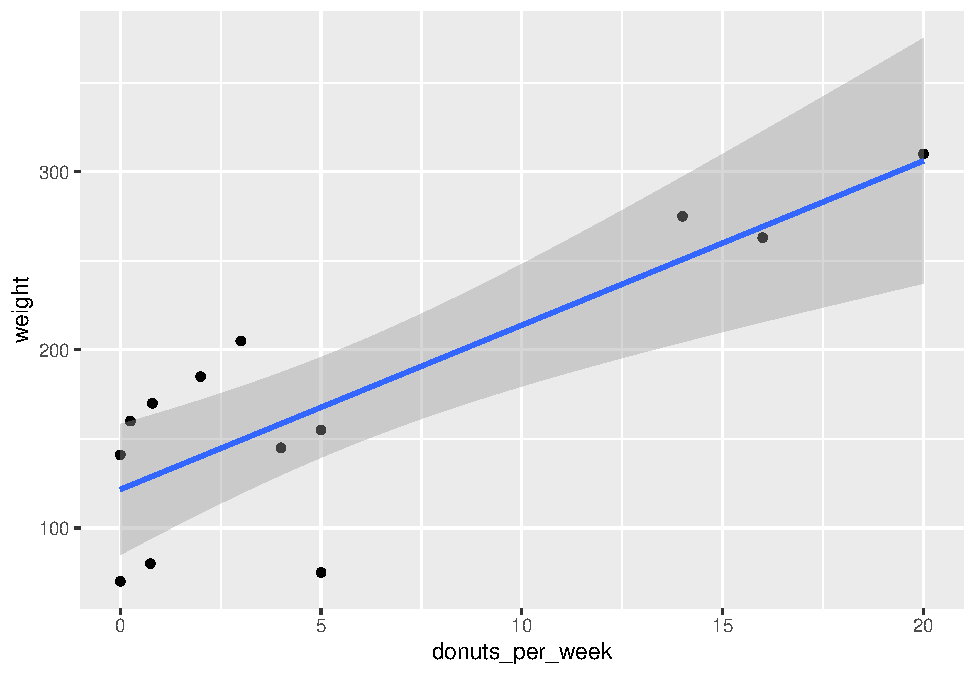
\includegraphics{bailey_files/figure-latex/unnamed-chunk-37-1.pdf}

\hypertarget{subsetting-data-for-regressions}{%
\section{Subsetting Data for Regressions}\label{subsetting-data-for-regressions}}

Subsetting can be directly done with the \texttt{subset} option in the \texttt{lm} call. To run a regression that excludes the Homer record, use the option \texttt{subset\ =\ (name\ !=\ "Homer")}.

\begin{Shaded}
\begin{Highlighting}[]
\NormalTok{ols_no_homer <-}\StringTok{ }\KeywordTok{lm}\NormalTok{(}\DataTypeTok{formula =}\NormalTok{ weight }\OperatorTok{~}\StringTok{ }\NormalTok{donuts_per_week, }\DataTypeTok{data =}\NormalTok{ donuts, }\DataTypeTok{subset =}\NormalTok{ (name }\OperatorTok{!=}\StringTok{ "Homer"}\NormalTok{))}
\NormalTok{ols_no_homer }\OperatorTok\StringTok{ }
\StringTok{  }\KeywordTok{tidy}\NormalTok{()}
\end{Highlighting}
\end{Shaded}

\begin{verbatim}
# A tibble: 2 x 5
  term            estimate std.error statistic   p.value
  <chr>              <dbl>     <dbl>     <dbl>     <dbl>
1 (Intercept)       122.       17.1       7.12 0.0000323
2 donuts_per_week     8.74      2.19      4.00 0.00252  
\end{verbatim}

\begin{Shaded}
\begin{Highlighting}[]
\NormalTok{ols_no_homer }\OperatorTok\StringTok{ }
\StringTok{  }\KeywordTok{summary}\NormalTok{()}
\end{Highlighting}
\end{Shaded}

\begin{verbatim}

Call:
lm(formula = weight ~ donuts_per_week, data = donuts, subset = (name != 
    "Homer"))

Residuals:
   Min     1Q Median     3Q    Max 
-90.58 -20.99   7.26  37.24  56.90 

Coefficients:
                Estimate Std. Error t value Pr(>|t|)    
(Intercept)       121.87      17.13    7.12 0.000032 ***
donuts_per_week     8.74       2.19    4.00   0.0025 ** 
---
Signif. codes:  0 '***' 0.001 '**' 0.01 '*' 0.05 '.' 0.1 ' ' 1

Residual standard error: 47.3 on 10 degrees of freedom
Multiple R-squared:  0.615, Adjusted R-squared:  0.577 
F-statistic:   16 on 1 and 10 DF,  p-value: 0.00252
\end{verbatim}

Alternatively we can make use of \texttt{filter} from the \texttt{dplyr} package. Recall, \texttt{filter} is the data manipulation verb that chooses observations in a data frame. I introduce the exposition operator \texttt{\%\$\%} from the magrittr package. \texttt{\%\$\%} is useful at the end of a pipeline to expose your manipulated data to function. You can use it with \texttt{subset} or \texttt{filter}.

\begin{Shaded}
\begin{Highlighting}[]
\NormalTok{donuts }\OperatorTok
\StringTok{  }\KeywordTok{subset}\NormalTok{(name }\OperatorTok{!=}\StringTok{ "Homer"}\NormalTok{) }\OperatorTok
\StringTok{  }\KeywordTok{lm}\NormalTok{(weight }\OperatorTok{~}\StringTok{ }\NormalTok{donuts_per_week)}
\end{Highlighting}
\end{Shaded}

\begin{verbatim}

Call:
lm(formula = weight ~ donuts_per_week)

Coefficients:
    (Intercept)  donuts_per_week  
         121.87             8.74  
\end{verbatim}

\begin{Shaded}
\begin{Highlighting}[]
\NormalTok{donuts }\OperatorTok
\StringTok{  }\KeywordTok{filter}\NormalTok{(name }\OperatorTok{!=}\StringTok{ "Homer"}\NormalTok{) }\OperatorTok
\StringTok{  }\KeywordTok{lm}\NormalTok{(weight }\OperatorTok{~}\StringTok{ }\NormalTok{donuts_per_week)}
\end{Highlighting}
\end{Shaded}

\begin{verbatim}

Call:
lm(formula = weight ~ donuts_per_week)

Coefficients:
    (Intercept)  donuts_per_week  
         121.87             8.74  
\end{verbatim}

To include those observations where weight is greater than 100:

\begin{Shaded}
\begin{Highlighting}[]
\NormalTok{donuts }\OperatorTok
\StringTok{  }\KeywordTok{subset}\NormalTok{(weight }\OperatorTok{>}\StringTok{ }\DecValTok{100}\NormalTok{) }\OperatorTok
\StringTok{  }\KeywordTok{lm}\NormalTok{(weight }\OperatorTok{~}\StringTok{ }\NormalTok{donuts_per_week)}
\end{Highlighting}
\end{Shaded}

\begin{verbatim}

Call:
lm(formula = weight ~ donuts_per_week)

Coefficients:
    (Intercept)  donuts_per_week  
         151.05             7.66  
\end{verbatim}

\begin{Shaded}
\begin{Highlighting}[]
\NormalTok{donuts }\OperatorTok
\StringTok{  }\KeywordTok{filter}\NormalTok{(weight }\OperatorTok{>}\StringTok{ }\DecValTok{100}\NormalTok{) }\OperatorTok
\StringTok{  }\KeywordTok{lm}\NormalTok{(weight }\OperatorTok{~}\StringTok{ }\NormalTok{donuts_per_week)}
\end{Highlighting}
\end{Shaded}

\begin{verbatim}

Call:
lm(formula = weight ~ donuts_per_week)

Coefficients:
    (Intercept)  donuts_per_week  
         151.05             7.66  
\end{verbatim}

\hypertarget{heteroscesdasticity-consistent-standard-errors.}{%
\section{Heteroscesdasticity-consistent standard errors.}\label{heteroscesdasticity-consistent-standard-errors.}}

The \texttt{estimatr} package allows you to directly calculate robust standard errors.

R Studio allows you to install packages in the Files/Plots/Packages/Help Pane by clicking on the Install icon on the Packages tab; as you type the name of the package, you will see completion suggestions. Choose the package you wish to install and R Studio will install it. You can load a package by checking the box next to its name in the Packages tab. Clicking on the packages name will bring up info about the pacakge.

Call \texttt{lm\_robust()} to estimate an OLS model with robust standard errors with the \texttt{se\_type\ =\ "HC0} option for the most common method of generating robust standard errors.

\begin{Shaded}
\begin{Highlighting}[]
\KeywordTok{library}\NormalTok{(estimatr)}
\NormalTok{ols_robust <-}\StringTok{ }\KeywordTok{lm_robust}\NormalTok{(weight }\OperatorTok{~}\StringTok{ }\NormalTok{donuts_per_week, donuts, }\DataTypeTok{se_type =} \StringTok{"HC0"}\NormalTok{)}
\NormalTok{ols_robust }\OperatorTok\StringTok{ }
\StringTok{  }\KeywordTok{tidy}\NormalTok{()}
\end{Highlighting}
\end{Shaded}

\begin{verbatim}
             term estimate std.error statistic    p.value conf.low
1     (Intercept)   121.61     15.87      7.66 0.00000983    86.68
2 donuts_per_week     9.22      1.02      9.07 0.00000194     6.99
  conf.high df outcome
1     156.5 11  weight
2      11.5 11  weight
\end{verbatim}

\hypertarget{generating-random-numbers}{%
\section{Generating Random Numbers}\label{generating-random-numbers}}

Random numbers can be useful in variety of applications in econometrics. One application is simulation, where we simulate observations to demonstrate properties of OLS estimators, eg. Once you've decided the distribution from which your random numbers will be drawn and the number of draws you wish to make, you will create a vector of those observations. The most intuitive form of random number generation is \texttt{sample}. Suppose you wanted to simulate the role of a single die, use \texttt{sample(1:6,1)} or using the pipe operator \texttt{1:6\ \%\textgreater{}\%\ sample(1)}. Read the command aloud like this ``from the integers 1, 2, 3, 4, 5, 6, choose a sample of size 1.'' You can choose larger samples by changing the size argument. The size argument can not be larger than the number of integers unless the default option of replace = FALSE, is changed to replace = TRUE. To generate a simulation of 100 rolls of a single die call \texttt{1:6\ \%\textgreater{}\%\ sample(100,\ replace\ =\ TRUE)}.

Random numbers may be generate from any probability distribution. The random number generator function for a given probability distribution begins with the letter r followed by the name of the distribution in r. To generate uniform random numbers between 0 and 1, use \texttt{runif}, from a normal distribution use \texttt{rnorm}, etc. Use \texttt{args(distribution\ name)} or \texttt{?distribution\ name} to find out more about the necessary arguments for individual distributions.

\hypertarget{simulations}{%
\section{Simulations}\label{simulations}}

Monte Carlo simulations are a useful tool for understanding how the value of an estimator changes as the sample data changes. Consider the example of rolling a single die n times and calculating the average number of pips on the side up face of the die. We know that \(\bar X\) is an ubiased estimator of \(\mu\). Recall that an estimator, \(\hat\theta\) is unbiased if \(E(\hat\theta) = \theta\). We can show that \(E(\bar X) = \mu\). Let \[\bar X = \frac{\sum{x_i}}{n}\]

Then, \[\begin{aligned}
E(\bar{X}) &= E\left( \frac{\sum{x_i}}{n} \right)\\
&= \frac{1}{n}\sum{E(x_i)} \\
&= \frac{1}{n}\sum{\mu}\\
&= \frac{1}{n}n\mu\\
&= \mu
\end{aligned}\]

So, we would expect \(\bar X = 3.5\) since \(\mu = 3.5\). Simulating 100 rolls of a single die 1000 times would allow us to look at the sampling distribution of the sample mean. This will allow us to see the range of values that \(\bar X\) might take on.

Perform a Monte Carlo simulation by generating many samples, find the value of the estimator, and investigate it's distribution. We could do this by generating a single sample, calculating the value of the estimator, and repeating the desired number of times. This would be tedious. We can instead make use of the concept of a loop in R. A loop evaluates the same code repeatedly until some threshold is met.

There are two types of loops in R, for loops and while loops. A for loop runs the code a specific number of times; a while loop runs the code until a logical condition is met. We will use a for loop to run our simulation. First, instruct R on the number of times to run through the loop. The loop itself is contained between the braces \{\}.

\begin{Shaded}
\begin{Highlighting}[]
\CommentTok{# library(tidyverse)}
\NormalTok{xbar <-}\StringTok{ }\DecValTok{1} \CommentTok{# initialize the vector to store the observations of x bar}
\ControlFlowTok{for}\NormalTok{(i }\ControlFlowTok{in} \DecValTok{1}\OperatorTok{:}\DecValTok{1000}\NormalTok{) \{}
\NormalTok{  x <-}\StringTok{ }\DecValTok{1}\OperatorTok{:}\DecValTok{6} \OperatorTok\StringTok{ }\KeywordTok{sample}\NormalTok{(}\DecValTok{100}\NormalTok{, }\DataTypeTok{replace =}\NormalTok{ T)}
\NormalTok{  xbar[i] <-}\StringTok{ }\KeywordTok{mean}\NormalTok{(x)}
\NormalTok{\}}
\NormalTok{xbar }\OperatorTok\StringTok{ }
\StringTok{  }\KeywordTok{mean}\NormalTok{() }\CommentTok{# find the mean of the 1000}
\end{Highlighting}
\end{Shaded}

\begin{verbatim}
[1] 3.51
\end{verbatim}

\begin{Shaded}
\begin{Highlighting}[]
\NormalTok{xbar }\OperatorTok
\StringTok{  }\KeywordTok{as.data.frame}\NormalTok{() }\OperatorTok\StringTok{ }\CommentTok{# coerce xbar to a data frame}
\StringTok{  }\KeywordTok{ggplot}\NormalTok{(}\KeywordTok{aes}\NormalTok{(}\DataTypeTok{x =}\NormalTok{ xbar)) }\OperatorTok{+}\StringTok{ }\CommentTok{# map xbar to x}
\StringTok{  }\KeywordTok{geom_density}\NormalTok{() }\OperatorTok{+}\StringTok{ }\CommentTok{# geom_density creates a "probability distribution"}
\StringTok{  }\KeywordTok{geom_vline}\NormalTok{(}\DataTypeTok{xintercept =} \FloatTok{3.5}\NormalTok{) }\CommentTok{# place a verticle line at the mean.}
\end{Highlighting}
\end{Shaded}

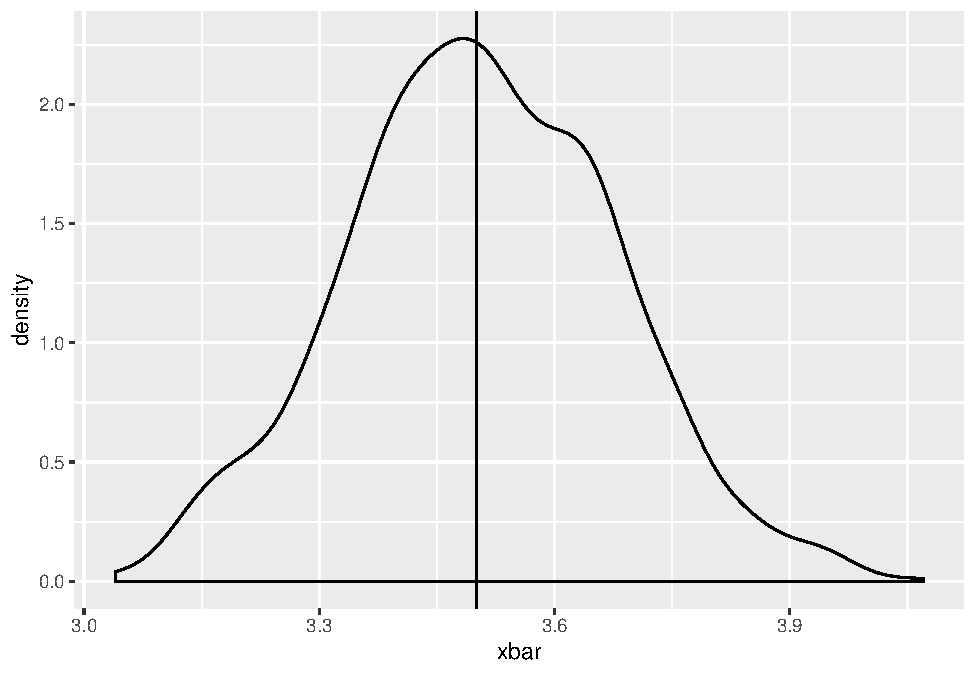
\includegraphics{bailey_files/figure-latex/unnamed-chunk-42-1.pdf}

We could do the same thing with the simple linear regression \(Y_i = \beta_0+\beta_1X_i+\epsilon_i\). We know the OLS estimator of \(\beta_1\) is \(\hat\beta_1\). The value of the estimator, called the estimate, depends upon the particular sample that is drawn. Monte Carlo simulation will allows to see how the estimate changes across many samples.

For \(\hat\beta_j\) to be an unbiased esitmator of \(\beta_j\), \(E(\hat\beta_j) = \beta_j\). The proof is beyond the scope of this manual, but you will see or have seen the proof.

Suppose we perform a Monte Carlo simulation with know values of \(\beta_0\) and \(\beta_1\) where the error term \(\epsilon_i\) is drawn from a normal distribution with a mean of zero and a constant variance, i.e., \(\epsilon_i ~ N(0, \sigma^2)\), will the estimates be statistically the same as the known parameters. Let's find out. Suppose the population regression function is \(y_i = 10 + 3x_i\),

\begin{Shaded}
\begin{Highlighting}[]
\NormalTok{n <-}\StringTok{ }\DecValTok{50}
\NormalTok{N <-}\StringTok{ }\DecValTok{1000} \CommentTok{# of simulations}
\NormalTok{beta_}\DecValTok{0}\NormalTok{ <-}\StringTok{ }\DecValTok{10}
\NormalTok{beta_}\DecValTok{1}\NormalTok{ <-}\StringTok{ }\DecValTok{3}
\NormalTok{beta_hat_}\DecValTok{0}\NormalTok{ <-}\StringTok{ }\DecValTok{0}
\NormalTok{beta_hat_}\DecValTok{1}\NormalTok{ <-}\StringTok{ }\DecValTok{0}
\NormalTok{y <-}\StringTok{ }\DecValTok{0}
\NormalTok{x <-}\StringTok{ }\DecValTok{1}\OperatorTok{:}\DecValTok{10} \OperatorTok\StringTok{ }\KeywordTok{sample}\NormalTok{(n, }\DataTypeTok{replace =}\NormalTok{ T) }\CommentTok{# we would determine x here if x were fixed in repeated sampling}
\ControlFlowTok{for}\NormalTok{(i }\ControlFlowTok{in} \DecValTok{1}\OperatorTok{:}\NormalTok{N) \{}
\NormalTok{ x <-}\StringTok{ }\DecValTok{0}\OperatorTok{:}\DecValTok{10} \OperatorTok\StringTok{ }\KeywordTok{sample}\NormalTok{(n, }\DataTypeTok{replace =}\NormalTok{ T)}
\NormalTok{ epsilon <-}\StringTok{ }\KeywordTok{rnorm}\NormalTok{(n, }\DecValTok{0}\NormalTok{ , }\DecValTok{2}\NormalTok{)}
\NormalTok{ y <-}\StringTok{  }\NormalTok{beta_}\DecValTok{0} \OperatorTok{+}\StringTok{ }\NormalTok{beta_}\DecValTok{1}\OperatorTok{*}\NormalTok{x }\OperatorTok{+}\StringTok{ }\NormalTok{epsilon}
\NormalTok{ beta_hat_}\DecValTok{0}\NormalTok{[i] <-}\StringTok{ }\KeywordTok{lm}\NormalTok{(y }\OperatorTok{~}\StringTok{ }\NormalTok{x)}\OperatorTok{$}\NormalTok{coef[}\DecValTok{1}\NormalTok{]}
\NormalTok{ beta_hat_}\DecValTok{1}\NormalTok{[i] <-}\StringTok{ }\KeywordTok{lm}\NormalTok{(y }\OperatorTok{~}\StringTok{ }\NormalTok{x)}\OperatorTok{$}\NormalTok{coef[}\DecValTok{2}\NormalTok{]}
\NormalTok{\}}
\CommentTok{#}
\NormalTok{beta_hat_}\DecValTok{0} \OperatorTok\StringTok{ }
\StringTok{  }\KeywordTok{mean}\NormalTok{()}
\end{Highlighting}
\end{Shaded}

\begin{verbatim}
[1] 9.98
\end{verbatim}

\begin{Shaded}
\begin{Highlighting}[]
\NormalTok{beta_hat_}\DecValTok{1} \OperatorTok\StringTok{ }
\StringTok{  }\KeywordTok{mean}\NormalTok{()}
\end{Highlighting}
\end{Shaded}

\begin{verbatim}
[1] 3
\end{verbatim}

\begin{Shaded}
\begin{Highlighting}[]
\NormalTok{beta_hat_}\DecValTok{0} \OperatorTok
\KeywordTok{as.data.frame}\NormalTok{() }\OperatorTok
\KeywordTok{ggplot}\NormalTok{(}\KeywordTok{aes}\NormalTok{(}\DataTypeTok{x =}\NormalTok{ beta_hat_}\DecValTok{0}\NormalTok{)) }\OperatorTok{+}
\KeywordTok{geom_density}\NormalTok{() }\OperatorTok{+}
\KeywordTok{geom_vline}\NormalTok{(}\DataTypeTok{xintercept =} \DecValTok{10}\NormalTok{)}
\end{Highlighting}
\end{Shaded}

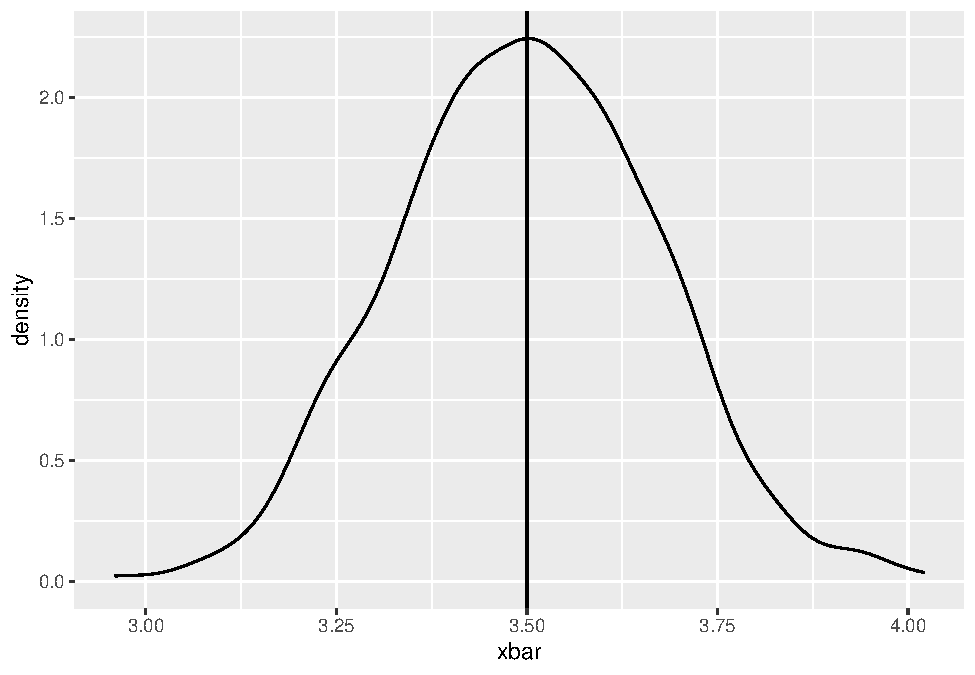
\includegraphics{bailey_files/figure-latex/unnamed-chunk-43-1.pdf}

\begin{Shaded}
\begin{Highlighting}[]
\NormalTok{beta_hat_}\DecValTok{1} \OperatorTok
\KeywordTok{as.data.frame}\NormalTok{() }\OperatorTok
\KeywordTok{ggplot}\NormalTok{(}\KeywordTok{aes}\NormalTok{(}\DataTypeTok{x =}\NormalTok{ beta_hat_}\DecValTok{1}\NormalTok{)) }\OperatorTok{+}
\KeywordTok{geom_density}\NormalTok{() }\OperatorTok{+}
\KeywordTok{geom_vline}\NormalTok{(}\DataTypeTok{xintercept =} \DecValTok{3}\NormalTok{)}
\end{Highlighting}
\end{Shaded}

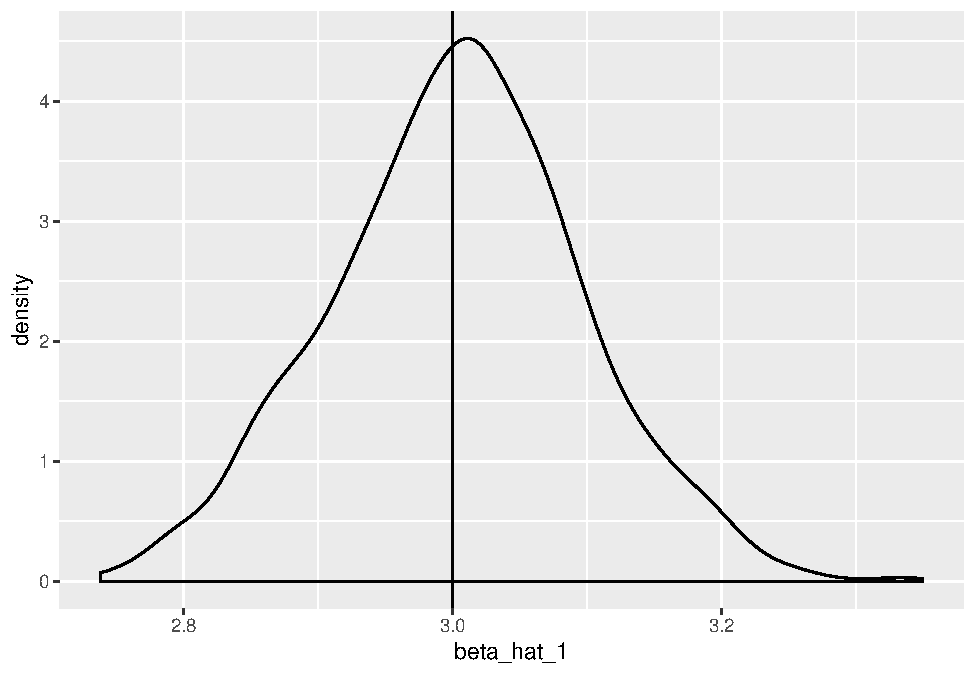
\includegraphics{bailey_files/figure-latex/unnamed-chunk-43-2.pdf}

\hypertarget{chp4}{%
\chapter{Hypothesis Testing and Interval Estimation; Answering Research Questions}\label{chp4}}

\hypertarget{computing-corner}{%
\section{Computing Corner}\label{computing-corner}}

We will learn the basisc for hypothesis testing in R.

\hypertarget{probability-distributions-in-r}{%
\subsection{Probability Distributions in R}\label{probability-distributions-in-r}}

For every probability distribution there are four commands. These command for each distribution are prepended by a letter to indicate the functionality.

\begin{itemize}
\tightlist
\item
  ``d'' returns the height of the probability ``d''ensity function
\item
  ``p'' returns the cummulative density function or the ``p''robability of being being between two values of the random variable.
\item
  ``q'' returns the inverse density function or the value of the random variable (``q''uantile) given a probability.
\item
  ``r'' returns a ``r''andomly generated number from the probability distribution
\end{itemize}

The distributions you are most likely to encounter in econometrics are the normal (norm), the F distribution (f), the chi-square distribution (chisq), and Student's t-distribution (t). Others include the uniform (unif), binomial (binom), Poisson (pois), etc. Use of the help tab in the Files/Plots/Packages/Help pane or use of \texttt{args} will list the arguments necessary to extract value for each distribution.

\hypertarget{critical-values-in-r}{%
\subsection{Critical Values in R}\label{critical-values-in-r}}

To calculate critical values to perform a hypothesis test use the ``q'' version of the probability distribution. This will return the quantile for the given probability. The probability under the curve will be cummulative from \(-\infty\) to the quantile returned. The ``q'' version will return the critical value for a one-tail test. Suppose you'd like to test the following hypothesis about \(\mu\):

\[H_0:\mu=0\]
\[H_1:\mu<0\]
at the \(\alpha=.05\) level of significance. To calculate the critical t-stastic call \texttt{qt(p\ =\ .05,\ df\ =\ n-1)}. You know from \texttt{args(qt)} the default value of the argument lower.tail is TRUE. Suppose, instead, you'd like to test the following hypothesis about \(\mu\)

\[H_0:\mu=0\]
\[H_1:\mu>0\]
at the \(\alpha = .10\) level of significance. You can call \texttt{qt} in two ways:

\begin{enumerate}
\def\labelenumi{\arabic{enumi}.}
\tightlist
\item
  \texttt{qt(p\ =\ .10,\ df\ =\ n-1,\ lower.tail\ =\ FALSE)} or
\item
  \texttt{qt(p\ =\ .90,\ df\ =\ n-1)}
\end{enumerate}

Finally, suppose you'd like to test the following hypothesis about \(\mu\)

\[H_0:\mu=0\]
\[H_1:\mu\ne0\]
at the \(\alpha=.01\) level of significance. Since the t-distribution is symmetric you can use the lower tail or upper tail value and -1 times it. You can call \texttt{qt} in three ways:

\begin{enumerate}
\def\labelenumi{\arabic{enumi}.}
\tightlist
\item
  \texttt{qt(p\ =\ .005,\ df\ =\ n-1)} or
\item
  \texttt{qt(p\ =\ .005,\ df\ =\ n-1,\ lower.tail\ =\ FALSE)} or
\item
  \texttt{qt(p\ =\ .995,\ df\ =\ n-1)}
\end{enumerate}

You can find crtical values for the normal, F, and \(\chi^2\) distributions with similar function calls.

\hypertarget{p-values-in-r}{%
\subsubsection{\texorpdfstring{\emph{p} values in R}{p values in R}}\label{p-values-in-r}}

To calculate \emph{p} values in R, use the ``p'' version of the distribution call. So suppose we test the following hypothesis:

\[H_0:\sigma_1^2=\sigma_2^2\]
\[H_0:\sigma_1^2\ne\sigma_2^2\]

at the \(\alpha=.05\) level of significance. We could use an F test of the form

\[F=\frac{s_x^2}{s_y^2}\]

where \(s_x^2\) and \(s_y^2\) are the sample variances with n-1 and m-1 degrees of freedom. To calculate the \emph{p} value, call \texttt{pf(F,\ n-1,\ m-1)} where F is the value calculated above.

\hypertarget{confidence-intervals-for-ols-estimates}{%
\subsection{Confidence Intervals for OLS estimates}\label{confidence-intervals-for-ols-estimates}}

In addition to \texttt{confint()}, \texttt{confint\_tidy()} from the broom package will create a tibble of the low and high values for each estimate. The default level of confidence is 95\%.

\hypertarget{power-curves}{%
\subsection{Power Curves}\label{power-curves}}

The power curve represents the probability of making Type II error under alternative null hypotheses. We can generate the power of the test with the \texttt{pwr.norm.test(d\ =\ NULL,\ n\ =\ NULL,\ sig.level\ =.05,\ power\ =\ NULL,\ alternative\ =\ c("two-sided",\ "less",\ "greater"))} call from the \texttt{pwr} package and plot the power with \texttt{ggplot}. To estimate the power we need the effect size \(d = \beta_i - \beta\) where \(\beta\) is the hypothesised paramater. We will use
\[H_0: \beta = 0\]
\[H_1: \beta > 0\]

The \(\beta_i\) represent alternative null hypothseses for \(\beta\). Let's let \(0 < beta < 7\). Let the significance level be \(\alpha=.01\) and \(se_{\beta} = 1\).

\begin{Shaded}
\begin{Highlighting}[]
\KeywordTok{library}\NormalTok{(tidyverse)}
\KeywordTok{library}\NormalTok{(pwr)}

\NormalTok{beta_i <-}\StringTok{ }\KeywordTok{seq}\NormalTok{(}\DecValTok{0}\NormalTok{, }\DecValTok{7}\NormalTok{, }\FloatTok{.1}\NormalTok{)}
\NormalTok{se_beta <-}\StringTok{ }\DecValTok{1} \CommentTok{# to keep se_beta = 1 we will set n = 1 below.}

\NormalTok{pwr <-}\StringTok{ }\KeywordTok{pwr.2p.test}\NormalTok{(beta_i, }\DataTypeTok{n =} \DecValTok{1}\NormalTok{, }\DataTypeTok{sig.level =} \FloatTok{.01}\NormalTok{, }\DataTypeTok{alternative =} \StringTok{"greater"}\NormalTok{)}

\CommentTok{#the output is a list we need to extract, h and power from pwr}

\NormalTok{data <-}\StringTok{ }\KeywordTok{tibble}\NormalTok{(}\DataTypeTok{beta =}\NormalTok{ pwr}\OperatorTok{$}\NormalTok{h, }\DataTypeTok{power =}\NormalTok{  pwr}\OperatorTok{$}\NormalTok{power)}

\NormalTok{data }\OperatorTok\StringTok{ }
\KeywordTok{ggplot}\NormalTok{(}\KeywordTok{aes}\NormalTok{(}\DataTypeTok{x =}\NormalTok{ beta, }\DataTypeTok{y =}\NormalTok{ power)) }\OperatorTok{+}
\StringTok{  }\KeywordTok{geom_line}\NormalTok{() }\OperatorTok{+}
\StringTok{  }\KeywordTok{ylab}\NormalTok{(}\StringTok{"Probability of rejecting the null"}\NormalTok{) }\OperatorTok{+}
\StringTok{  }\KeywordTok{xlab}\NormalTok{(}\KeywordTok{expression}\NormalTok{(beta))}
\end{Highlighting}
\end{Shaded}

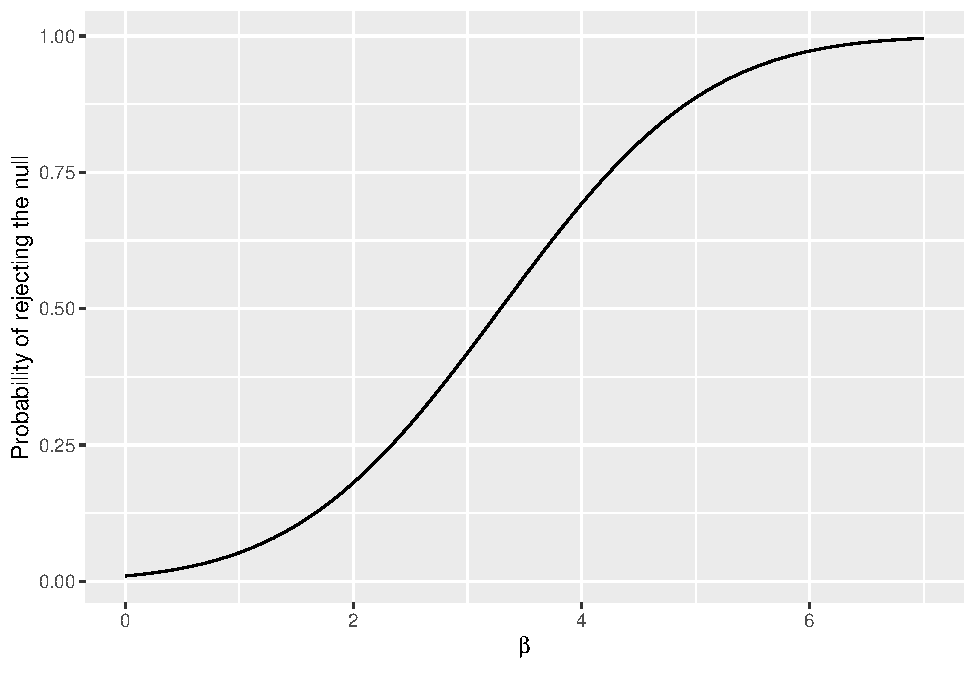
\includegraphics{bailey_files/figure-latex/power-1.pdf}

\hypertarget{chp5}{%
\chapter{Multivariate OLS: Where the Action Is}\label{chp5}}

\hypertarget{computing-corner-1}{%
\section{Computing Corner}\label{computing-corner-1}}

Packages needed for this chapter.

\begin{Shaded}
\begin{Highlighting}[]
\KeywordTok{library}\NormalTok{(magrittr)}
\KeywordTok{library}\NormalTok{(car)}
\KeywordTok{library}\NormalTok{(broom)}
\KeywordTok{library}\NormalTok{(estimatr)}
\KeywordTok{library}\NormalTok{(lm.beta)}
\end{Highlighting}
\end{Shaded}

In this chapter you will learn the basics of estimating multivariate OLS models.

\hypertarget{multiple-regression}{%
\subsection{Multiple Regression}\label{multiple-regression}}

To estitmate a multiple regression (a regression with more than one independent variable) use the same function \texttt{lm} but change the formula argument to include the additional variables. In a simple regression, the formula argument was of the form \texttt{y\ \textasciitilde{}\ x}. In a multiple regression, the formula argument takes the form \texttt{y\ \textasciitilde{}\ x1\ +\ x2}. To include additional variables, extend the argument in a similar manner \texttt{y\ \textasciitilde{}\ x1\ +\ x2\ +\ x3\ +\ ...}. The remaining arguments are the same as in the simple regression. You can assign the results to an object just as with a simple regression. The output will be the list of 12, but the objects in the list will change to reflect the additional variable(s).

To make use of the results, you can use any of the functions described in Chapter 3 of this manual. You can also make use of any of the subsetting commands as well.

Estimate a regression with robust standard errors with \texttt{lm\_robust} with the modified function argument.

\hypertarget{multicollinearity}{%
\subsection{Multicollinearity}\label{multicollinearity}}

You can directly estimate the VIF's with the \texttt{vif()} function from the car package. To esitmate the VIF's call \texttt{ols\ \%\textgreater{}\%\ vif()} where ols is the object you created with the \texttt{lm} call.

\hypertarget{standardized-coefficients}{%
\subsection{Standardized Coefficients}\label{standardized-coefficients}}

Estimate standardized regression coefficients with \texttt{lm.beta()} from the lm.beta package. \texttt{ols\ \%\textgreater{}\%\ lm.beta()}.

\hypertarget{f-tests}{%
\subsection{\texorpdfstring{\emph{F} tests}{F tests}}\label{f-tests}}

\emph{F} tests in econometrics are generally about the joint significance of multiple variables. Suppose, we estimate the regression on \(i=1,2,\ldots n\) observations. \[y_i=\beta_0+\beta_1x_{1,i}+\beta_2x_{2,i}+\cdots+\beta_mx_{i,m}+\beta_{m+1}x_{m+1,i}+\cdots+\beta_kx_{i,k} + \epsilon_i\]

To test the joint significance of the \(\beta_1,\ldots,\beta_m\) in the model we would use an \emph{F} test to perform the following hypothesis test: \[H_0: \beta_1=\beta_2=\cdots=\beta_m=0\] \[H_1:\text{@ least one }\beta_j\ne0\]

An \emph{F} test essentially compares the difference in the residual sum of squares under the null and alternative hypotheses. If this difference in large enough relative to the unrestricted standard error, we have evidence to reject the null hypothesis in favor of the alternative hypothesis. The mechanics of the test are as follows:

\begin{enumerate}
\def\labelenumi{\arabic{enumi}.}
\item
  Estimate the model that does not hold under the null hypothesis, that is, the model above and call it the unsrestricted model and retrieve the residual sum of squares. Retrieve the residual sum of squares, \(rss_u\). The residuals from unrestricted model will have \(n-k-1\) degrees of freedom. The unrestricted model, U, is: \[\text{U: }y_i=\beta_0+\beta_1x_{1,i}+\beta_2x_{2,i}+\cdots+\beta_mx_{i,m}+\beta_{m+1}x_{m+1,i}+\cdots+\beta_kx_{i,k} + \epsilon_i\]
\item
  Estimate the model that holds under the null hypothesis Restrict the model so that the null hypothesis holds. That restricted model, R, is \[\text{R: }y_i=\beta_0+\beta_{m+1}x_{m+1,i}+\beta_{m+2}x_{m+2,i}+\cdots+\beta_kx_{k,i} + \eta_i\]. Retrieve the residual sum of squares \(rss_r\) The residual from restricted model will have \(n-m-1\) degrees of freedom.
\item
  Calculate the difference in the residual sum of squares \(rss_r - rss_u\) and divide by its degrees of of freedom \(q = (n-m-1)-(n-k-1) = k-m\). So, q is the number of restrictions. A simple way to calculate the number of restrictions is to count the number of equal signs, \(=\), in the null hypothesis.
\item
  Calculate \(rss_u/(n-k-1)\)
\item
  Divide the result from 3 by the result from 4. This will give you an \emph{F} statistic with k-m and n-k-1 degrees of freedom.
\end{enumerate}

\[F_c=\frac{\frac{rss_r-rss_u}{q}}{\frac{rss_u}{n-k-1}}\]

The \emph{F}-test (Wald test) can be used for any number of restrictions on the unrestricted model. For example, suppose we would like to know if a production function with a Cobb-Douglas form has constant returns to scale. The Cobb-Douglas function for output as a function of labor and capital takes the form \[q=al^\alpha k^\beta\epsilon\]. If constant returns to scale hold, \(\alpha+\beta=1\). So we test the following hypothesis: \[H_0:\alpha+\beta=1\] \[H_1:\alpha+\beta\ne1\]

To test this hypothesis form the unrestricted and restricted forms of the model, estimate the models, retrieve the sum of squared residuals, and calculate the \emph{F} statistic. In the form presented above, the Cobb-Douglas model is not linear in the parameters so it can't be estimated with OLS. We can make it linear in the parameters by taking the logarithm of both sides. \[\ln(q)=\ln(al^\alpha k^\beta\epsilon)\] \[\text{U: }\ln(q)=\gamma+\alpha \ln(l)+\beta\ln(k)+\eta\].

Form the restricted model by emposing the null hypothesis on the paramaters. From the null hypothesis, \(\beta=1-\alpha\). Substituting for \(\beta\) in the restricted model yields the restricted model. \[\text{R: }\ln(q)-\ln(k)=\gamma+\alpha[\ln(l)-\ln(k)]+\eta\]

The \emph{F}-stat is: \[F_c=\frac{rss_r-rss_u}{\frac{rss_u}{n-k-1}}\]

The degrees of freedom are \(q=1\) (the number of equal signs in the null hypothesis) and \(n-k-1\).

\hypertarget{f-test-for-overall-significance.}{%
\subsubsection{\texorpdfstring{\emph{F}-test for overall significance.}{F-test for overall significance.}}\label{f-test-for-overall-significance.}}

Estimate the model \(y_i=\beta_0+\beta_1x_{1,i}+\beta_2x_{2,i}+\cdots+\beta_kx_{k,i}+\epsilon_i\). Test the hypothesis \[H_0: \beta_1=\beta_2=\cdots=\beta_k=0\] \[H_1:\text{@ least one }\beta_j\ne0\]

If we reject the null hypothesis, we can say that we have explained some varation in \(y\) with variation in at least one of the \(x's\). In other words, we have a model that is significant. If we fail to reject the null hypothesis, our model has no explanatory power. There is no need to calculate the \emph{F}-statistic to perform this test because it is reported as a matter of course in the base R call \texttt{summary} or in \texttt{glance} from the broom package. The degrees of freedom are \(q=k\) (the number of coefficients estimated - 1) and \(n-k-1\).

\texttt{summary} will report the F-statistic, its degrees of freedom (numerator and denominator), and the p-value. \texttt{glance} reports the \emph{F} as ``statistic'', the p-value as ``p.value'', \(k+1\) as ``df'', and \(n-k-1\) as ``df.residual''. Note that this test is also a test for the significance of \(R^2\).

\hypertarget{f-test-of-linear-restrictions}{%
\subsubsection{\texorpdfstring{\emph{F}-test of linear restrictions}{F-test of linear restrictions}}\label{f-test-of-linear-restrictions}}

The test we performed above are tests of linear restrictions of the parameters. These hypotheses can be tested directly using \texttt{linearHypothesis} from the car package. Performing a test of linear restrictions using \texttt{linearHypothesis} requires two arguments: model and hypothesis.matrix.

Let the unrestricted model be \[y=\beta_0+\beta_1x_1+\beta_2x_2+\beta_3x_3+\epsilon\] Estimate the model as \texttt{ols\_u\ \textless{}-\ df\ \%\$\%\ lm(y\ \textasciitilde{}\ x1\ +\ x2\ +\ x3)}, where df is the data frame containing the data.

Let's test the hypothesis \(\beta_2=\beta_3=0\) versus at that one of the \(\beta's\ne0\) using \texttt{linearHypothesis(model\ =\ ols\_u,\ hypothesis.matrix\ =\ c("x2\ =\ 0",\ "x3\ =\ 0")}. The result will be an \emph{F}-test on the restrictions. The \emph{F}-statistic, its degrees of freedom, and p-value will be returned.

Let's test the linear restriction for the Cobb-Douglas model above. Estimate the model as \texttt{ols\_u\ \textless{}-\ df\ \%\$\%\ lm(log(q)\ \textasciitilde{}\ log(l)\ +\ log(k))}. To test the hypothesis \(\alpha=\beta\) pipe ols\_u into \texttt{linearHypothesis} with the argument \(c(log(l) = log(k))\): \texttt{ols\_u\ \%\textgreater{}\%\ linearHypothesis(c("log(l)\ =\ log(k)"))}. Again, the \emph{F}-statistic, its degrees of freedom, and p-value will be returned.

\hypertarget{examples}{%
\subsection{Examples}\label{examples}}

The Motor Trend Car Road Test (mtcars) data set is part of the datasets in base R. The data were extracted from the 1974 Motor Trend US magazine, and comprises fuel consumption and 10 aspects of automobile design and performance for 32 automobiles (1973-74 models). See \texttt{?mtcars} for more information on the data. \texttt{data(mtcars)} will load the data into your global environment as mtcars. We will perform each of the \emph{F}-tests described above: overall significance, joint signficance of a subset of variables, and equality of two coefficients.

\hypertarget{multiple-regression-1}{%
\subsubsection{Multiple Regression}\label{multiple-regression-1}}

Suppose we want to estimate the mpg as a function of the number of cylinders, the displacement, and the gross horsepower, then our (unrestricted) model is \[mpg=\beta_0+\beta_1cyl+\beta_2disp+\beta_3hp+\epsilon\].

Let's estimate the unrestricted model using the expose pipe \texttt{\%\$\%} both with and without robust errors.

\begin{Shaded}
\begin{Highlighting}[]
\CommentTok{# estimate model without reobust standard errors}
\NormalTok{ols <-}\StringTok{ }\NormalTok{mtcars }\OperatorTok\StringTok{ }\KeywordTok{lm}\NormalTok{(mpg }\OperatorTok{~}\StringTok{ }\NormalTok{cyl }\OperatorTok{+}\StringTok{ }\NormalTok{disp }\OperatorTok{+}\StringTok{ }\NormalTok{hp)}
\NormalTok{ols }\OperatorTok\StringTok{ }\KeywordTok{tidy}\NormalTok{()}
\end{Highlighting}
\end{Shaded}

\begin{verbatim}
# A tibble: 4 x 5
  term        estimate std.error statistic  p.value
  <chr>          <dbl>     <dbl>     <dbl>    <dbl>
1 (Intercept)  34.2       2.59       13.2  1.54e-13
2 cyl          -1.23      0.797      -1.54 1.35e- 1
3 disp         -0.0188    0.0104     -1.81 8.09e- 2
4 hp           -0.0147    0.0147     -1.00 3.25e- 1
\end{verbatim}

\begin{Shaded}
\begin{Highlighting}[]
\CommentTok{# estimate model with robust standard erros}
\NormalTok{ols_robust <-}\StringTok{ }\NormalTok{mtcars }\OperatorTok\StringTok{ }\KeywordTok{lm_robust}\NormalTok{(mpg }\OperatorTok{~}\StringTok{ }\NormalTok{cyl }\OperatorTok{+}\StringTok{ }\NormalTok{disp }\OperatorTok{+}\StringTok{ }\NormalTok{hp)}
\NormalTok{ols_robust }\OperatorTok\StringTok{  }\KeywordTok{tidy}\NormalTok{()}
\end{Highlighting}
\end{Shaded}

\begin{verbatim}
         term estimate std.error statistic           p.value conf.low
1 (Intercept)  34.1849    2.4700     13.84 0.000000000000048  29.1253
2         cyl  -1.2274    0.5967     -2.06 0.049121075438813  -2.4498
3        disp  -0.0188    0.0083     -2.27 0.031138440490781  -0.0358
4          hp  -0.0147    0.0109     -1.34 0.190818678697032  -0.0371
  conf.high df outcome
1  39.24451 28     mpg
2  -0.00506 28     mpg
3  -0.00183 28     mpg
4   0.00775 28     mpg
\end{verbatim}

\hypertarget{multicollinearity-1}{%
\subsubsection{Multicollinearity}\label{multicollinearity-1}}

Using the model above \[mpg=\beta_0+\beta_1cyl+\beta_2disp+\beta_3hp+\epsilon\].

We can calcualte the VIF's as follows:

\begin{Shaded}
\begin{Highlighting}[]
\NormalTok{ols }\OperatorTok\StringTok{ }\KeywordTok{vif}\NormalTok{()}
\end{Highlighting}
\end{Shaded}

\begin{verbatim}
 cyl disp   hp 
6.73 5.52 3.35 
\end{verbatim}

\begin{Shaded}
\begin{Highlighting}[]
\NormalTok{ols_robust }\OperatorTok\StringTok{ }\KeywordTok{vif}\NormalTok{()}
\end{Highlighting}
\end{Shaded}

\begin{verbatim}
 cyl disp   hp 
3.67 2.90 2.71 
\end{verbatim}

\hypertarget{standardize-regression-coefficients}{%
\subsubsection{Standardize Regression Coefficients}\label{standardize-regression-coefficients}}

Using the model \[mpg=\beta_0+\beta_1cyl+\beta_2disp+\beta_3hp+\epsilon\], estimate standardized regression coefficients as follows:

\begin{Shaded}
\begin{Highlighting}[]
\NormalTok{ols }\OperatorTok\StringTok{ }\KeywordTok{lm.beta}\NormalTok{()}
\end{Highlighting}
\end{Shaded}

\begin{verbatim}

Call:
lm(formula = mpg ~ cyl + disp + hp)

Standardized Coefficients::
(Intercept)         cyl        disp          hp 
      0.000      -0.364      -0.387      -0.167 
\end{verbatim}

\hypertarget{f-test-for-overall-significance}{%
\subsubsection{\texorpdfstring{\emph{F}-test for Overall significance}{F-test for Overall significance}}\label{f-test-for-overall-significance}}

Suppose we want to estimate the mpg as a function of the number of cylinders, the displacement, and the gross horsepower, then our (unrestricted) model is \[mpg=\beta_0+\beta_1cyl+\beta_2disp+\beta_3hp+\epsilon\].

Let's estimate the unrestricted model using the expose pipe \texttt{\%\$\%}

\begin{Shaded}
\begin{Highlighting}[]
\NormalTok{ols_u <-}\StringTok{ }\NormalTok{mtcars }\OperatorTok\StringTok{ }\KeywordTok{lm}\NormalTok{(mpg }\OperatorTok{~}\StringTok{ }\NormalTok{cyl }\OperatorTok{+}\StringTok{ }\NormalTok{disp }\OperatorTok{+}\StringTok{ }\NormalTok{hp)}
\end{Highlighting}
\end{Shaded}

The test for overall significance is: \[H_0:\beta_1=\beta_2=\beta_3=0\] \[H_1: \text{@ least one }\beta_j\ne0\]

Recall that \emph{the} \emph{F}-test is reported as a matter of course in \texttt{summary} from base R and \texttt{glance} from the broom package.

\begin{Shaded}
\begin{Highlighting}[]
\NormalTok{ols_u }\OperatorTok\StringTok{ }\KeywordTok{summary}\NormalTok{()}
\end{Highlighting}
\end{Shaded}

\begin{verbatim}

Call:
lm(formula = mpg ~ cyl + disp + hp)

Residuals:
   Min     1Q Median     3Q    Max 
-4.089 -2.085 -0.774  1.397  6.918 

Coefficients:
            Estimate Std. Error t value         Pr(>|t|)    
(Intercept)  34.1849     2.5908   13.19 0.00000000000015 ***
cyl          -1.2274     0.7973   -1.54            0.135    
disp         -0.0188     0.0104   -1.81            0.081 .  
hp           -0.0147     0.0147   -1.00            0.325    
---
Signif. codes:  0 '***' 0.001 '**' 0.01 '*' 0.05 '.' 0.1 ' ' 1

Residual standard error: 3.06 on 28 degrees of freedom
Multiple R-squared:  0.768, Adjusted R-squared:  0.743 
F-statistic: 30.9 on 3 and 28 DF,  p-value: 0.00000000505
\end{verbatim}

\begin{Shaded}
\begin{Highlighting}[]
\NormalTok{ols_u }\OperatorTok\StringTok{ }\KeywordTok{glance}\NormalTok{()}
\end{Highlighting}
\end{Shaded}

\begin{verbatim}
# A tibble: 1 x 11
  r.squared adj.r.squared sigma statistic p.value    df logLik   AIC   BIC
      <dbl>         <dbl> <dbl>     <dbl>   <dbl> <int>  <dbl> <dbl> <dbl>
1     0.768         0.743  3.06      30.9 5.05e-9     4  -79.0  168.  175.
# ... with 2 more variables: deviance <dbl>, df.residual <int>
\end{verbatim}

So we see that \(F=30.877\), \(q=3\), and \(df2=28\). The critical \emph{F} with \(\alpha=.05\) is \(2.947\). Since the calculated \emph{F}-stat is greater than the critical \emph{F}-stat, we reject \(H_0\) in favor of \(H_1\). That is, the explanatory power of the model is statistical significant.

\hypertarget{f-test-of-joint-significance}{%
\subsubsection{\texorpdfstring{\emph{F}-test of Joint Significance}{F-test of Joint Significance}}\label{f-test-of-joint-significance}}

Suppose we'd like to add the weight (wt), number of gears (gear), and number of carburetors (carb) together increase the explanatory power of the model at the \(\alpha=.05\), level of significance. Our unrestricted model becomes: \[mpg=\beta_0+\beta_1cyl+\beta_2disp+\beta_3hp+\beta_4wt+\beta_5gear+\beta_6carb+\eta\].

The null and alternative hypotheses are: \[H_0:\beta_4=\beta_5=\beta_6=0\] \[H_1:\text{@ least one }\beta_j\ne0\]

\hypertarget{perform-the-test-manually}{%
\subsubsection{Perform the test ``manually''}\label{perform-the-test-manually}}

\begin{Shaded}
\begin{Highlighting}[]
\CommentTok{# estimate the unrestricted model}
\NormalTok{ols_u <-}\StringTok{ }\NormalTok{mtcars }\OperatorTok\StringTok{ }\KeywordTok{lm}\NormalTok{(mpg }\OperatorTok{~}\StringTok{ }\NormalTok{cyl }\OperatorTok{+}\StringTok{ }\NormalTok{disp }\OperatorTok{+}\StringTok{ }\NormalTok{disp }\OperatorTok{+}\StringTok{ }\NormalTok{hp }\OperatorTok{+}\StringTok{ }\NormalTok{wt }\OperatorTok{+}\StringTok{ }\NormalTok{gear }\OperatorTok{+}\StringTok{ }\NormalTok{carb)}
\CommentTok{# generate the residual sum of squares}
\NormalTok{rss_u <-}\StringTok{ }\NormalTok{ols_u}\OperatorTok{$}\NormalTok{residuals}\OperatorTok{^}\DecValTok{2} \OperatorTok\StringTok{ }
\StringTok{  }\KeywordTok{sum}\NormalTok{()}
\CommentTok{# retrive the degrees of freedom for the unrestricted model}
\NormalTok{df_u <-}\StringTok{ }\NormalTok{ols_u}\OperatorTok{$}\NormalTok{df.residual}
\CommentTok{# estimate the restricted model}
\NormalTok{ols_r <-}\StringTok{ }\NormalTok{mtcars }\OperatorTok\StringTok{ }\KeywordTok{lm}\NormalTok{(mpg }\OperatorTok{~}\StringTok{ }\NormalTok{cyl }\OperatorTok{+}\StringTok{ }\NormalTok{disp }\OperatorTok{+}\StringTok{ }\NormalTok{disp }\OperatorTok{+}\StringTok{ }\NormalTok{hp)}
\CommentTok{# generate the residual sum of squares}
\NormalTok{rss_r <-}\StringTok{ }\NormalTok{ols_r}\OperatorTok{$}\NormalTok{residuals}\OperatorTok{^}\DecValTok{2} \OperatorTok\StringTok{ }
\StringTok{  }\KeywordTok{sum}\NormalTok{()}
\CommentTok{# retrive the degrees of freedom for the restricted model}
\NormalTok{df_r <-}\StringTok{ }\NormalTok{ols_r}\OperatorTok{$}\NormalTok{df.residual}
\CommentTok{# calculate the number of restrictions}
\NormalTok{q <-}\StringTok{ }\NormalTok{df_r }\OperatorTok{-}\StringTok{ }\NormalTok{df_u}
\CommentTok{# calculate F}
\NormalTok{(F_stat <-}\StringTok{ }\NormalTok{((rss_r}\OperatorTok{-}\NormalTok{rss_u)}\OperatorTok{/}\NormalTok{q)}\OperatorTok{/}\NormalTok{(rss_u}\OperatorTok{/}\NormalTok{df_u)) }\CommentTok{# () around the call prints the result to the screen}
\end{Highlighting}
\end{Shaded}

\begin{verbatim}
[1] 4.8
\end{verbatim}

\begin{Shaded}
\begin{Highlighting}[]
\CommentTok{# retrieve the critical F}
\NormalTok{(F_crit <-}\StringTok{ }\KeywordTok{qf}\NormalTok{(.}\DecValTok{95}\NormalTok{, q, df_u))}
\end{Highlighting}
\end{Shaded}

\begin{verbatim}
[1] 2.99
\end{verbatim}

\begin{Shaded}
\begin{Highlighting}[]
\CommentTok{# p-value }
\NormalTok{(F_stat }\OperatorTok\StringTok{ }\KeywordTok{pf}\NormalTok{(q, df_u, }\DataTypeTok{lower.tail =}\NormalTok{ F))}
\end{Highlighting}
\end{Shaded}

\begin{verbatim}
[1] 0.00897
\end{verbatim}

Since 4.796 is greater than 2.991 we can reject \(H_0\) in favor of \(H_1\) and conclude that wt, am, and carb add signficant explanatory power to the model. We can also see that the p-vallue for our calculated \emph{F}-statistic is 0.009. Since this is less than \(\alpha=.05\) we reject \(H_0\).

\hypertarget{perform-the-test-with-linearhypothesis}{%
\subsubsection{\texorpdfstring{Perform the test with \texttt{linearHypothesis}}{Perform the test with linearHypothesis}}\label{perform-the-test-with-linearhypothesis}}

\begin{Shaded}
\begin{Highlighting}[]
\KeywordTok{linearHypothesis}\NormalTok{(ols_u, }\KeywordTok{c}\NormalTok{(}\StringTok{"wt"}\NormalTok{, }\StringTok{"gear"}\NormalTok{, }\StringTok{"carb"}\NormalTok{))}
\end{Highlighting}
\end{Shaded}

\begin{verbatim}
Linear hypothesis test

Hypothesis:
wt = 0
gear = 0
carb = 0

Model 1: restricted model
Model 2: mpg ~ cyl + disp + disp + hp + wt + gear + carb

  Res.Df RSS Df Sum of Sq   F Pr(>F)   
1     28 261                           
2     25 166  3      95.5 4.8  0.009 **
---
Signif. codes:  0 '***' 0.001 '**' 0.01 '*' 0.05 '.' 0.1 ' ' 1
\end{verbatim}

Of course, we have the same result.

\hypertarget{test-of-linear-restrictions}{%
\subsubsection{Test of Linear Restrictions}\label{test-of-linear-restrictions}}

Let the model be \[\ln(mpg)=\beta_0+\beta_1\ln(cyl)+\beta_2\ln(wt)+\epsilon\]. Suppose we'd like to test \[H_0:\beta_1+\beta_2=-1\] against \[H_0:\beta_1+\beta_2\ne-1\]

\hypertarget{perform-the-test-manually-1}{%
\paragraph{Perform the Test ``Manually''}\label{perform-the-test-manually-1}}

Form the restricted model under \(H_0\). If \(H_0\) holds, \(\beta_2=-1-\beta_1\). Substituting into the unrestricted model yields the restricted model: \[\text{R: }\ln(mpg)+\ln(wt)=\beta_0+\beta_1(\ln(cyl)-\ln(wt))+\eta\]

\begin{Shaded}
\begin{Highlighting}[]
\CommentTok{# estimate the unrestricted model}
\NormalTok{ols_u <-}\StringTok{ }\NormalTok{mtcars }\OperatorTok\StringTok{ }\KeywordTok{lm}\NormalTok{(}\KeywordTok{log}\NormalTok{(mpg) }\OperatorTok{~}\StringTok{ }\KeywordTok{log}\NormalTok{(cyl) }\OperatorTok{+}\StringTok{ }\KeywordTok{log}\NormalTok{(wt))}
\CommentTok{# generate the residual sum of squares}
\NormalTok{rss_u <-}\StringTok{ }\NormalTok{ols_u}\OperatorTok{$}\NormalTok{residuals}\OperatorTok{^}\DecValTok{2} \OperatorTok\StringTok{ }
\StringTok{  }\KeywordTok{sum}\NormalTok{()}
\CommentTok{# retrive the degrees of freedom for the unrestricted model}
\NormalTok{df_u <-}\StringTok{ }\NormalTok{ols_u}\OperatorTok{$}\NormalTok{df.residual}
\CommentTok{# estimate the restricted model}
\NormalTok{ols_r <-}\StringTok{ }\NormalTok{mtcars }\OperatorTok\StringTok{ }\KeywordTok{lm}\NormalTok{(}\KeywordTok{I}\NormalTok{(}\KeywordTok{log}\NormalTok{(mpg)}\OperatorTok{+}\KeywordTok{log}\NormalTok{(wt)) }\OperatorTok{~}\StringTok{ }\KeywordTok{I}\NormalTok{(}\KeywordTok{log}\NormalTok{(cyl) }\OperatorTok{-}\StringTok{ }\KeywordTok{log}\NormalTok{(wt)))}
\CommentTok{# generate the residual sum of squares}
\NormalTok{rss_r <-}\StringTok{ }\NormalTok{ols_r}\OperatorTok{$}\NormalTok{residuals}\OperatorTok{^}\DecValTok{2} \OperatorTok\StringTok{ }
\StringTok{  }\KeywordTok{sum}\NormalTok{()}
\CommentTok{# retrive the degrees of freedom for the restricted model}
\NormalTok{df_r <-}\StringTok{ }\NormalTok{ols_r}\OperatorTok{$}\NormalTok{df.residual}
\CommentTok{# calculate the number of restrictions}
\NormalTok{q <-}\StringTok{ }\NormalTok{df_r }\OperatorTok{-}\StringTok{ }\NormalTok{df_u}
\CommentTok{# calculate F}
\NormalTok{(F_stat <-}\StringTok{ }\NormalTok{((rss_r}\OperatorTok{-}\NormalTok{rss_u)}\OperatorTok{/}\NormalTok{q)}\OperatorTok{/}\NormalTok{(rss_u}\OperatorTok{/}\NormalTok{df_u)) }\CommentTok{# () around the call prints the result to the screen}
\end{Highlighting}
\end{Shaded}

\begin{verbatim}
[1] 1.29
\end{verbatim}

\begin{Shaded}
\begin{Highlighting}[]
\CommentTok{# retrieve the critical F}
\NormalTok{(F_crit <-}\StringTok{ }\KeywordTok{qf}\NormalTok{(.}\DecValTok{95}\NormalTok{, q, df_u))}
\end{Highlighting}
\end{Shaded}

\begin{verbatim}
[1] 4.18
\end{verbatim}

\begin{Shaded}
\begin{Highlighting}[]
\CommentTok{# p-value }
\NormalTok{(F_stat }\OperatorTok\StringTok{ }\KeywordTok{pf}\NormalTok{(q, df_u, }\DataTypeTok{lower.tail =}\NormalTok{ F))}
\end{Highlighting}
\end{Shaded}

\begin{verbatim}
[1] 0.266
\end{verbatim}

Since 1.289 is less than 4.183 we can failt to reject \(H_0\) and conclude that we have no evidence to suggest that \(\beta_1+\beta_2\ne1\). We can also see that the p-vallue for our calculated \emph{F}-statistic is 0.266. Since this is greater than \(\alpha=.05\) we fail to reject \(H_0\).

\hypertarget{perform-the-test-with-linearhypothesis-1}{%
\subsubsection{\texorpdfstring{Perform the test with \texttt{linearHypothesis}}{Perform the test with linearHypothesis}}\label{perform-the-test-with-linearhypothesis-1}}

\begin{Shaded}
\begin{Highlighting}[]
\NormalTok{ols_u }\OperatorTok\StringTok{ }\KeywordTok{linearHypothesis}\NormalTok{(}\KeywordTok{c}\NormalTok{(}\StringTok{"log(cyl) + log(wt) = -1"}\NormalTok{))}
\end{Highlighting}
\end{Shaded}

\begin{verbatim}
Linear hypothesis test

Hypothesis:
log(cyl)  + log(wt) = - 1

Model 1: restricted model
Model 2: log(mpg) ~ log(cyl) + log(wt)

  Res.Df   RSS Df Sum of Sq    F Pr(>F)
1     30 0.419                         
2     29 0.401  1    0.0178 1.29   0.27
\end{verbatim}

\hypertarget{chp6}{%
\chapter{Dummy Variables: Smarter than You Think}\label{chp6}}

In this chapter we will learn how R handles dummy variables.

We will need the following libraries.

\begin{Shaded}
\begin{Highlighting}[]
\KeywordTok{library}\NormalTok{(tidyverse)}
\KeywordTok{library}\NormalTok{(magrittr)}
\KeywordTok{library}\NormalTok{(broom)}
\KeywordTok{library}\NormalTok{(estimatr)}
\KeywordTok{library}\NormalTok{(forcats)}
\end{Highlighting}
\end{Shaded}

\hypertarget{dummy-variables-in-r}{%
\section{Dummy Variables in R}\label{dummy-variables-in-r}}

R uses factor vectors to to represent dummy or categorical data. Factors can be ordered or unordered. Factor vectors are built on top of integer vectors and include a unique label for each integer.

\hypertarget{factors}{%
\subsection{Factors}\label{factors}}

R uses factors to handle categorical variables. Categorical variables have fixed and known set of possible values. The package \href{https://forcats.tidyverse.org/}{forcats} as part of the tidyverse offers a suite of tools for that solve common problems with factors. See the \href{https://forcats.tidyverse.org/articles/forcats.html}{vignette on forcats} for more information on the forcats package to learn more about using factors in R.

\hypertarget{character-vectors-as-dummies}{%
\subsection{Character Vectors as Dummies}\label{character-vectors-as-dummies}}

Character vectors are one of the six atomic vector types in R. \emph{Atomic} means that the vector contains only data of a single type, in this case all of the observations are characters. Categorical data or dummy variables though they are typically coded as numeric are character vectors. For example, a dummy varialbe for sex may contain male and female, but be coded as 0 and 1 and named female. If you use a character vector as an argument in \texttt{lm}, R will treat the vector as a set of dummy variables. The number of dummy variables will be the number of characteristics (unique observations) minus 1.

The student admissions at UC Berkeley data set has aggregate data on graduate school applicants for the six largest departments, \texttt{?UCBAdmissions} for more information. There are four variables in the data set, Admit (whether the cadidate was admitted or rejected), Gender (the gender of the candidate: Male or Female), Dept (department to which the candidate applied coded as A, B, C, D, E, F), and n (the number of applicants). n is a numeric vector. Admit, Gender, and Dept, are character vectors. Since the data are store as a table, to read them into R as a data frame call \texttt{as\_tibble} from the dplyr package with the argument UCBAdmissions.

\begin{Shaded}
\begin{Highlighting}[]
\NormalTok{UCB_Admissions <-}\StringTok{ }\NormalTok{UCBAdmissions }\OperatorTok\StringTok{ }
\StringTok{  }\KeywordTok{as_tibble}\NormalTok{() }\OperatorTok\StringTok{  }
\StringTok{  }\KeywordTok{glimpse}\NormalTok{() }
\end{Highlighting}
\end{Shaded}

\begin{verbatim}
Observations: 24
Variables: 4
$ Admit  <chr> "Admitted", "Rejected", "Admitted", "Rejected", "Admitt...
$ Gender <chr> "Male", "Male", "Female", "Female", "Male", "Male", "Fe...
$ Dept   <chr> "A", "A", "A", "A", "B", "B", "B", "B", "C", "C", "C", ...
$ n      <dbl> 512, 313, 89, 19, 353, 207, 17, 8, 120, 205, 202, 391, ...
\end{verbatim}

Suppose we wisht to estimate the difference in difference model \(n_i = \beta_0+\beta_1Admit_i+\epsilon_i\). If we use Admit as an argument in \texttt{lm}, R will correctly treat Admit as single dummy variable with two categories.

\begin{Shaded}
\begin{Highlighting}[]
\NormalTok{UCB_Admissions }\OperatorTok
\StringTok{  }\KeywordTok{lm}\NormalTok{(n }\OperatorTok{~}\StringTok{ }\NormalTok{Admit)}
\end{Highlighting}
\end{Shaded}

\begin{verbatim}

Call:
lm(formula = n ~ Admit)

Coefficients:
  (Intercept)  AdmitRejected  
        146.2           84.7  
\end{verbatim}

R has coded Rejected as 1 and Admitted as 0. The regression indicates that mean of admitted is 146.25 while the mean number rejected is 230.92. We can confirm that directly as well.

\begin{Shaded}
\begin{Highlighting}[]
\CommentTok{# Using dplyr verbs}
\NormalTok{UCB_Admissions }\OperatorTok\StringTok{ }
\StringTok{  }\KeywordTok{filter}\NormalTok{(Admit }\OperatorTok{==}\StringTok{ "Admitted"}\NormalTok{) }\OperatorTok\StringTok{ }
\StringTok{  }\KeywordTok{summary}\NormalTok{(mean) }
\end{Highlighting}
\end{Shaded}

\begin{verbatim}
    Admit              Gender              Dept                 n      
 Length:12          Length:12          Length:12          Min.   : 17  
 Class :character   Class :character   Class :character   1st Qu.: 46  
 Mode  :character   Mode  :character   Mode  :character   Median :107  
                                                          Mean   :146  
                                                          3rd Qu.:154  
                                                          Max.   :512  
\end{verbatim}

\begin{Shaded}
\begin{Highlighting}[]
\NormalTok{UCB_Admissions }\OperatorTok\StringTok{ }
\StringTok{  }\KeywordTok{filter}\NormalTok{(Admit }\OperatorTok{==}\StringTok{ "Rejected"}\NormalTok{) }\OperatorTok\StringTok{ }
\StringTok{  }\KeywordTok{summary}\NormalTok{(mean)}
\end{Highlighting}
\end{Shaded}

\begin{verbatim}
    Admit              Gender              Dept                 n      
 Length:12          Length:12          Length:12          Min.   :  8  
 Class :character   Class :character   Class :character   1st Qu.:188  
 Mode  :character   Mode  :character   Mode  :character   Median :262  
                                                          Mean   :231  
                                                          3rd Qu.:314  
                                                          Max.   :391  
\end{verbatim}

\begin{Shaded}
\begin{Highlighting}[]
\CommentTok{# Directly selecting observations based on other values}
\NormalTok{UCB_Admissions }\OperatorTok\StringTok{ }
\StringTok{  }\KeywordTok{mean}\NormalTok{(n[Admit }\OperatorTok{==}\StringTok{ "Admitted"}\NormalTok{])}
\end{Highlighting}
\end{Shaded}

\begin{verbatim}
[1] 146
\end{verbatim}

\begin{Shaded}
\begin{Highlighting}[]
\NormalTok{UCB_Admissions }\OperatorTok\StringTok{ }
\StringTok{  }\KeywordTok{mean}\NormalTok{(n[Admit }\OperatorTok{==}\StringTok{ "Rejected"}\NormalTok{])}
\end{Highlighting}
\end{Shaded}

\begin{verbatim}
[1] 231
\end{verbatim}

Similarly, if we want to calculate the mean number of applicants by department, R will treat Dept as 5 dummy variables.

\begin{Shaded}
\begin{Highlighting}[]
\NormalTok{UCB_Admissions }\OperatorTok
\StringTok{  }\KeywordTok{lm}\NormalTok{(n }\OperatorTok{~}\StringTok{ }\NormalTok{Dept) }
\end{Highlighting}
\end{Shaded}

\begin{verbatim}

Call:
lm(formula = n ~ Dept)

Coefficients:
(Intercept)        DeptB        DeptC        DeptD        DeptE  
     233.25       -87.00        -3.75       -35.25       -87.25  
      DeptF  
     -54.75  
\end{verbatim}

The mean number of applicants in Department A is 233.25. To find the mean number of applicants for each department add the appropriate coefficient to 233.25.

We can confirm these results as we did above.

\hypertarget{difference-in-means-test}{%
\section{Difference in Means Test}\label{difference-in-means-test}}

Using the UCB Admissions data, let's conduct a difference of means test for number of applications by Gender. We will test the following hypothesis: \[H_0: \mu_{Male}=\mu_{Female}\\ H_1: \mu_{Male}\ne\mu_{Female}\] at the \(\alpha=.05\) level of significance. We can use \texttt{t.test} in two different ways, \texttt{lm}, or \texttt{lm\_robust}. First, we will test the hypothesis with \texttt{t.test} assuming, in turn, equal and unequal variances.

\hypertarget{using-t.test}{%
\subsection{\texorpdfstring{Using \texttt{t.test}}{Using t.test}}\label{using-t.test}}

\begin{Shaded}
\begin{Highlighting}[]
\CommentTok{# Assume equal variances}
\CommentTok{# Use t.test default method}
\NormalTok{UCB_Admissions }\OperatorTok
\StringTok{  }\KeywordTok{t.test}\NormalTok{(n[Gender }\OperatorTok{==}\StringTok{ "Female"}\NormalTok{], n[Gender }\OperatorTok{==}\StringTok{ "Male"}\NormalTok{], }\DataTypeTok{var.equal =} \OtherTok{TRUE}\NormalTok{)}
\end{Highlighting}
\end{Shaded}

\begin{verbatim}

    Two Sample t-test

data:  n[Gender == "Female"] and n[Gender == "Male"]
t = -1, df = 22, p-value = 0.2
alternative hypothesis: true difference in means is not equal to 0
95 percent confidence interval:
 -188.4   45.7
sample estimates:
mean of x mean of y 
      153       224 
\end{verbatim}

\begin{Shaded}
\begin{Highlighting}[]
\CommentTok{# Use t.test for class 'formula`}
\NormalTok{UCB_Admissions }\OperatorTok
\StringTok{  }\KeywordTok{t.test}\NormalTok{(n }\OperatorTok{~}\StringTok{ }\NormalTok{Gender, }\DataTypeTok{var.equal =} \OtherTok{TRUE}\NormalTok{)}
\end{Highlighting}
\end{Shaded}

\begin{verbatim}

    Two Sample t-test

data:  n by Gender
t = -1, df = 22, p-value = 0.2
alternative hypothesis: true difference in means is not equal to 0
95 percent confidence interval:
 -188.4   45.7
sample estimates:
mean in group Female   mean in group Male 
                 153                  224 
\end{verbatim}

\begin{Shaded}
\begin{Highlighting}[]
\CommentTok{# Assume unequal variances}
\CommentTok{# unequal variances is the default}
\NormalTok{UCB_Admissions }\OperatorTok
\StringTok{  }\KeywordTok{t.test}\NormalTok{(n[Gender }\OperatorTok{==}\StringTok{ "Female"}\NormalTok{], n[Gender }\OperatorTok{==}\StringTok{ "Male"}\NormalTok{])}
\end{Highlighting}
\end{Shaded}

\begin{verbatim}

    Welch Two Sample t-test

data:  n[Gender == "Female"] and n[Gender == "Male"]
t = -1, df = 22, p-value = 0.2
alternative hypothesis: true difference in means is not equal to 0
95 percent confidence interval:
 -188.4   45.8
sample estimates:
mean of x mean of y 
      153       224 
\end{verbatim}

\begin{Shaded}
\begin{Highlighting}[]
\CommentTok{# Use t.test for class 'formula`}
\NormalTok{UCB_Admissions }\OperatorTok
\StringTok{  }\KeywordTok{t.test}\NormalTok{(n }\OperatorTok{~}\StringTok{ }\NormalTok{Gender)}
\end{Highlighting}
\end{Shaded}

\begin{verbatim}

    Welch Two Sample t-test

data:  n by Gender
t = -1, df = 22, p-value = 0.2
alternative hypothesis: true difference in means is not equal to 0
95 percent confidence interval:
 -188.4   45.8
sample estimates:
mean in group Female   mean in group Male 
                 153                  224 
\end{verbatim}

\hypertarget{using-lm-and-lm_robust}{%
\subsection{\texorpdfstring{Using \texttt{lm} and \texttt{lm\_robust}}{Using lm and lm\_robust}}\label{using-lm-and-lm_robust}}

\begin{Shaded}
\begin{Highlighting}[]
\CommentTok{# Assume equal variances}
\NormalTok{UCB_Admissions }\OperatorTok
\StringTok{  }\KeywordTok{lm}\NormalTok{(n }\OperatorTok{~}\StringTok{ }\NormalTok{Gender) }\OperatorTok\StringTok{ }
\StringTok{  }\KeywordTok{tidy}\NormalTok{()}
\end{Highlighting}
\end{Shaded}

\begin{verbatim}
# A tibble: 2 x 5
  term        estimate std.error statistic  p.value
  <chr>          <dbl>     <dbl>     <dbl>    <dbl>
1 (Intercept)    153.       39.9      3.83 0.000911
2 GenderMale      71.3      56.5      1.26 0.220   
\end{verbatim}

\begin{Shaded}
\begin{Highlighting}[]
\CommentTok{# Assume unequal variances}
\NormalTok{UCB_Admissions }\OperatorTok
\StringTok{  }\KeywordTok{lm_robust}\NormalTok{(n }\OperatorTok{~}\StringTok{ }\NormalTok{Gender) }\OperatorTok\StringTok{ }
\StringTok{  }\KeywordTok{tidy}\NormalTok{()}
\end{Highlighting}
\end{Shaded}

\begin{verbatim}
         term estimate std.error statistic  p.value conf.low conf.high df
1 (Intercept)    152.9      38.7      3.95 0.000679     72.7       233 22
2  GenderMale     71.3      56.5      1.26 0.219606    -45.7       188 22
  outcome
1       n
2       n
\end{verbatim}

\hypertarget{integer-and-numerical-vectors-as-dummy-variables}{%
\section{Integer and Numerical Vectors as Dummy Variables}\label{integer-and-numerical-vectors-as-dummy-variables}}

\texttt{lm} treated the character vectors as factors. For most of what we will do, that is enough. If the categorical (dummy) variable is coded as a numeric vector or integer vector, we my have coerce the variable to a factor for \texttt{lm} to interpret it correctly. If the variable is coded as 0 and 1, we can use it as it is. For example, conisder the the mtcars data.

\begin{Shaded}
\begin{Highlighting}[]
\KeywordTok{data}\NormalTok{(mtcars)}
\NormalTok{mtcars }\OperatorTok\StringTok{ }\KeywordTok{glimpse}\NormalTok{()}
\end{Highlighting}
\end{Shaded}

\begin{verbatim}
Observations: 32
Variables: 11
$ mpg  <dbl> 21.0, 21.0, 22.8, 21.4, 18.7, 18.1, 14.3, 24.4, 22.8, 19....
$ cyl  <dbl> 6, 6, 4, 6, 8, 6, 8, 4, 4, 6, 6, 8, 8, 8, 8, 8, 8, 4, 4, ...
$ disp <dbl> 160.0, 160.0, 108.0, 258.0, 360.0, 225.0, 360.0, 146.7, 1...
$ hp   <dbl> 110, 110, 93, 110, 175, 105, 245, 62, 95, 123, 123, 180, ...
$ drat <dbl> 3.90, 3.90, 3.85, 3.08, 3.15, 2.76, 3.21, 3.69, 3.92, 3.9...
$ wt   <dbl> 2.62, 2.88, 2.32, 3.21, 3.44, 3.46, 3.57, 3.19, 3.15, 3.4...
$ qsec <dbl> 16.5, 17.0, 18.6, 19.4, 17.0, 20.2, 15.8, 20.0, 22.9, 18....
$ vs   <dbl> 0, 0, 1, 1, 0, 1, 0, 1, 1, 1, 1, 0, 0, 0, 0, 0, 0, 1, 1, ...
$ am   <dbl> 1, 1, 1, 0, 0, 0, 0, 0, 0, 0, 0, 0, 0, 0, 0, 0, 0, 1, 1, ...
$ gear <dbl> 4, 4, 4, 3, 3, 3, 3, 4, 4, 4, 4, 3, 3, 3, 3, 3, 3, 4, 4, ...
$ carb <dbl> 4, 4, 1, 1, 2, 1, 4, 2, 2, 4, 4, 3, 3, 3, 4, 4, 4, 1, 2, ...
\end{verbatim}

The type of transmission, am, takes on two values 1 if the transmission is automatic and 0 if it is manual. Suppose we'd like to know if the mpg is different for the two types of transmissions. We can test the hypothesis \[H_0:\mu_a=\mu_m\] \[H_1:\mu_a\ne\mu_m\]d at the \(\alpha=.05\) level of significance.

\begin{Shaded}
\begin{Highlighting}[]
\NormalTok{mtcars }\OperatorTok
\StringTok{  }\KeywordTok{lm_robust}\NormalTok{(mpg }\OperatorTok{~}\StringTok{ }\NormalTok{am) }\OperatorTok\StringTok{ }
\StringTok{  }\KeywordTok{tidy}\NormalTok{()}
\end{Highlighting}
\end{Shaded}

\begin{verbatim}
         term estimate std.error statistic                p.value conf.low
1 (Intercept)    17.15      0.88     19.50 0.00000000000000000138    15.35
2          am     7.24      1.92      3.77 0.00072109506857981581     3.32
  conf.high df outcome
1      18.9 30     mpg
2      11.2 30     mpg
\end{verbatim}

If, however, the categorical variable is not coded as 0 and 1, we will have to coerce it to a factor. The forcats package simplifies this process. Suppose we'd like to know if the average mpg is different for 4, 6, and 8 cylinder cars. \[H_0:\mu_4=\mu_6=\mu_8\] \[H_1:\text{@ least one }\mu\text{ is not equal}\]If we estimate a model of mpg on cyl, the coefficient on cyl will give us the marginal effect on mpg of adding a cylinder. A signficant coefficient in this model will not answer our question. To do that, we must coerce cyl into a categorical variable with \texttt{as.factor}.

\begin{Shaded}
\begin{Highlighting}[]
\NormalTok{mtcars }\OperatorTok
\StringTok{  }\KeywordTok{lm}\NormalTok{(mpg }\OperatorTok{~}\StringTok{ }\KeywordTok{as.factor}\NormalTok{(cyl)) }\OperatorTok\StringTok{ }
\StringTok{  }\KeywordTok{summary}\NormalTok{()}
\end{Highlighting}
\end{Shaded}

\begin{verbatim}

Call:
lm(formula = mpg ~ as.factor(cyl))

Residuals:
   Min     1Q Median     3Q    Max 
-5.264 -1.836  0.029  1.389  7.236 

Coefficients:
                Estimate Std. Error t value             Pr(>|t|)    
(Intercept)       26.664      0.972   27.44 < 0.0000000000000002 ***
as.factor(cyl)6   -6.921      1.558   -4.44              0.00012 ***
as.factor(cyl)8  -11.564      1.299   -8.90        0.00000000086 ***
---
Signif. codes:  0 '***' 0.001 '**' 0.01 '*' 0.05 '.' 0.1 ' ' 1

Residual standard error: 3.22 on 29 degrees of freedom
Multiple R-squared:  0.732, Adjusted R-squared:  0.714 
F-statistic: 39.7 on 2 and 29 DF,  p-value: 0.00000000498
\end{verbatim}

The \emph{F-stat} for overall significance of the model is significant at the \(\alpha = .05\) level of significance so we reject the null hypothesis in favor of the alternative and conclude that at least one average mpg is different.

The base case is cars with 4 cylinders with an average mpg of 26.7 mpg. 6 cylinder cars average a statistically significant 6.9 mpg less than 4 cylinder cars. 8 cylinder cars average a statistically siginficant 11.6 mpg less than 4 cylider cars. These averages are statistically signficantly different.

Had we estimated the model without coercing cylinders into a factor our results would have been

\begin{Shaded}
\begin{Highlighting}[]
\NormalTok{mtcars }\OperatorTok\StringTok{ }
\StringTok{  }\KeywordTok{lm}\NormalTok{(mpg }\OperatorTok{~}\StringTok{ }\NormalTok{cyl) }\OperatorTok\StringTok{ }
\StringTok{  }\KeywordTok{tidy}\NormalTok{()}
\end{Highlighting}
\end{Shaded}

\begin{verbatim}
# A tibble: 2 x 5
  term        estimate std.error statistic  p.value
  <chr>          <dbl>     <dbl>     <dbl>    <dbl>
1 (Intercept)    37.9      2.07      18.3  8.37e-18
2 cyl            -2.88     0.322     -8.92 6.11e-10
\end{verbatim}

\(\hat\beta_1=-2.88\) tells us that for each additional cylinder fuel mileage will fall by 2.88 mpg.

\hypertarget{manipulating-factors}{%
\section{Manipulating Factors}\label{manipulating-factors}}

The forcats package provides a set of tools for the simple manipulation of factors like renaming factors, re-ordering factors, combining factors, etc. Using the mtcars data, lets coerce the number of cylinders to a factor and look at ways to manipulate in ways to aid in understanding. The compound pipe operator \texttt{\%\textless{}\textgreater{}\%} is used to update a value by first piping into one or more expressions and then assigning the result.

\begin{Shaded}
\begin{Highlighting}[]
\KeywordTok{data}\NormalTok{(mtcars)}
\CommentTok{### Coerce cyl to a factor}
\NormalTok{mtcars}\OperatorTok{$}\NormalTok{cyl }\OperatorTok\StringTok{ }
\StringTok{  }\KeywordTok{as.character}\NormalTok{() }\OperatorTok\StringTok{ }\CommentTok{# forcats will not coerce integer or numeric vectors to factors}
\StringTok{  }\KeywordTok{as_factor}\NormalTok{()}
\NormalTok{mtcars}\OperatorTok{$}\NormalTok{cyl }\OperatorTok\StringTok{ }\KeywordTok{str}\NormalTok{()}
\end{Highlighting}
\end{Shaded}

\begin{verbatim}
 Factor w/ 3 levels "6","4","8": 1 1 2 1 3 1 3 2 2 1 ...
\end{verbatim}

cyl is now a factor with 3 levels, 6, 4, 8. Suppose we estimate the model \(mpg = \beta_0 + \beta_1mpg+\epsilon\).

\begin{Shaded}
\begin{Highlighting}[]
\NormalTok{mtcars }\OperatorTok\StringTok{ }
\StringTok{  }\KeywordTok{lm}\NormalTok{(mpg }\OperatorTok{~}\StringTok{ }\NormalTok{cyl) }\OperatorTok\StringTok{ }
\StringTok{  }\KeywordTok{tidy}\NormalTok{()}
\end{Highlighting}
\end{Shaded}

\begin{verbatim}
# A tibble: 3 x 5
  term        estimate std.error statistic  p.value
  <chr>          <dbl>     <dbl>     <dbl>    <dbl>
1 (Intercept)    19.7       1.22     16.2  4.49e-16
2 cyl4            6.92      1.56      4.44 1.19e- 4
3 cyl8           -4.64      1.49     -3.11 4.15e- 3
\end{verbatim}

This model indicates that cars with 6 cylinder engines average 19.74 mpg, cars with 4 cylinders average 6.9 mpg more than cars with 6 cylinders, and cars with 8 cylinders average 4.64 mpg less than cars with 6 cylinders. Suppose, instead, you'd prefere 4 cylinder cars to be the base case. We can reorder the factor with \texttt{fct\_relevel} from the forcats package. \texttt{fct\_revel} changes the order of a factor by hand.

For some factors the order doesn't or won't matter, for others there is ``natural'' ordering suggested by the data, for others you may have an ordering that you prefer. \texttt{fct\_relevel()} from the forcats package handles that task. If we call \texttt{fct\_relevel} within \texttt{lm} the releveling will be \emph{ad hoc}.

\begin{Shaded}
\begin{Highlighting}[]
\NormalTok{mtcars }\OperatorTok
\StringTok{  }\KeywordTok{lm}\NormalTok{(mpg }\OperatorTok{~}\StringTok{ }\KeywordTok{fct_relevel}\NormalTok{(cyl, }\DataTypeTok{levels =} \KeywordTok{c}\NormalTok{(}\StringTok{"4"}\NormalTok{, }\StringTok{"6"}\NormalTok{, }\StringTok{"8"}\NormalTok{))) }\OperatorTok\StringTok{ }
\StringTok{  }\KeywordTok{tidy}\NormalTok{()}
\end{Highlighting}
\end{Shaded}

\begin{verbatim}
# A tibble: 3 x 5
  term                                estimate std.error statistic  p.value
  <chr>                                  <dbl>     <dbl>     <dbl>    <dbl>
1 (Intercept)                            26.7      0.972     27.4  2.69e-22
2 "fct_relevel(cyl, levels = c(\"4\"~    -6.92     1.56      -4.44 1.19e- 4
3 "fct_relevel(cyl, levels = c(\"4\"~   -11.6      1.30      -8.90 8.57e-10
\end{verbatim}

We can permantly relevel cylinders

\begin{Shaded}
\begin{Highlighting}[]
\CommentTok{# relevel the factor}
\NormalTok{mtcars}\OperatorTok{$}\NormalTok{cyl  <-}\StringTok{ }
\StringTok{  }\KeywordTok{fct_relevel}\NormalTok{(mtcars}\OperatorTok{$}\NormalTok{cyl, }\DataTypeTok{levels =} \KeywordTok{c}\NormalTok{(}\StringTok{"4"}\NormalTok{, }\StringTok{"6"}\NormalTok{, }\StringTok{"8"}\NormalTok{))}
\CommentTok{# alternatively }
\NormalTok{mtcars}\OperatorTok{$}\NormalTok{cyl <-}\StringTok{ }
\StringTok{  }\KeywordTok{fct_relevel}\NormalTok{(mtcars}\OperatorTok{$}\NormalTok{cyl, }\StringTok{"6"}\NormalTok{, }\DataTypeTok{after =} \DecValTok{1}\NormalTok{) }\CommentTok{# move 6 to the second position}
\CommentTok{# re-estimate the model}
\NormalTok{mtcars }\OperatorTok
\StringTok{  }\KeywordTok{lm}\NormalTok{(mpg }\OperatorTok{~}\StringTok{ }\NormalTok{cyl) }\OperatorTok\StringTok{ }
\StringTok{  }\KeywordTok{tidy}\NormalTok{()}
\end{Highlighting}
\end{Shaded}

\begin{verbatim}
# A tibble: 3 x 5
  term        estimate std.error statistic  p.value
  <chr>          <dbl>     <dbl>     <dbl>    <dbl>
1 (Intercept)    26.7      0.972     27.4  2.69e-22
2 cyl6           -6.92     1.56      -4.44 1.19e- 4
3 cyl8          -11.6      1.30      -8.90 8.57e-10
\end{verbatim}

See \href{https://forcats.tidyverse.org/reference/fct_relevel.html}{Reorder factor levels by hand} for a more ways to relevel factors.

The transmission variable (am) is a numeric vector coded as 0 and 1. Suppose we'd like to coerce it to a factor coded with the levels named ``automatic'' and ``manual'' rather than 0 and 1.

\begin{Shaded}
\begin{Highlighting}[]
\NormalTok{mtcars}\OperatorTok{$}\NormalTok{am }\OperatorTok\StringTok{ }
\StringTok{  }\KeywordTok{factor}\NormalTok{(}\DataTypeTok{levels =} \KeywordTok{c}\NormalTok{(}\DecValTok{0}\NormalTok{,}\DecValTok{1}\NormalTok{), }\DataTypeTok{labels =} \KeywordTok{c}\NormalTok{(}\StringTok{"automatic"}\NormalTok{, }\StringTok{"manual"}\NormalTok{))}
\end{Highlighting}
\end{Shaded}

If we re-estimate the model \(mpg = \beta_0+\beta_1am\) we see the results are the same, but the variable is labeled more clearly.

\begin{Shaded}
\begin{Highlighting}[]
\NormalTok{mtcars }\OperatorTok
\StringTok{  }\KeywordTok{lm_robust}\NormalTok{(mpg }\OperatorTok{~}\StringTok{ }\NormalTok{am) }\OperatorTok\StringTok{ }
\StringTok{  }\KeywordTok{tidy}\NormalTok{()}
\end{Highlighting}
\end{Shaded}

\begin{verbatim}
         term estimate std.error statistic                p.value conf.low
1 (Intercept)    17.15      0.88     19.50 0.00000000000000000138    15.35
2    ammanual     7.24      1.92      3.77 0.00072109506857981581     3.32
  conf.high df outcome
1      18.9 30     mpg
2      11.2 30     mpg
\end{verbatim}

\hypertarget{dummy-interaction-variables}{%
\section{Dummy Interaction Variables}\label{dummy-interaction-variables}}

Dummy interactions \(x_iD_i\) can be created in \texttt{lm} as an argument. Let's esitmate the the model \(mpg= \beta_0+\beta_1am+\beta_2hp+\beta_3hp*am+\epsilon\).

\begin{Shaded}
\begin{Highlighting}[]
\NormalTok{mtcars }\OperatorTok
\StringTok{  }\KeywordTok{lm}\NormalTok{(mpg }\OperatorTok{~}\StringTok{ }\NormalTok{hp}\OperatorTok{*}\NormalTok{am) }
\end{Highlighting}
\end{Shaded}

\begin{verbatim}

Call:
lm(formula = mpg ~ hp * am)

Coefficients:
(Intercept)           hp     ammanual  hp:ammanual  
  26.624848    -0.059137     5.217653     0.000403  
\end{verbatim}

Notice that R assumed that you wanted to calculate \(\hat\beta_1\), \(\hat\beta_2\), and \(\hat\beta_3\). By including \texttt{hp*am} as an argument in \texttt{lm} R estimated the continuous coefficients for the continuous variable, the dummy variable, and the interactions. If, on the other hand, you wanted just the interaction term, i.e., \(mpg=\alpha_0+\alpha_1hp*am+\eta\), use the ``AsIs'' function \texttt{I()} as follows:

\begin{Shaded}
\begin{Highlighting}[]
\KeywordTok{data}\NormalTok{(mtcars)}
\NormalTok{mtcars }\OperatorTok
\StringTok{  }\KeywordTok{lm}\NormalTok{(mpg }\OperatorTok{~}\StringTok{ }\KeywordTok{I}\NormalTok{(hp}\OperatorTok{*}\NormalTok{am))}
\end{Highlighting}
\end{Shaded}

\begin{verbatim}

Call:
lm(formula = mpg ~ I(hp * am))

Coefficients:
(Intercept)   I(hp * am)  
    19.5696       0.0101  
\end{verbatim}

\texttt{I()} is used to inhibit the interpretation of operators in formulas, so they are used as arithmetic operators.

\hypertarget{chp7}{%
\chapter{Specifying Models}\label{chp7}}

In addition to its role in limiting endogeneity, model specification plays an important role in modeling in economics. The defining characteristic of economic reasoning is marginalism so having functional forms that make marginal sense is important. In this chapter we will learn to estimate some important functional forms in economics.

We will use the following libraries.

\begin{Shaded}
\begin{Highlighting}[]
\KeywordTok{library}\NormalTok{(tidyverse)}
\KeywordTok{library}\NormalTok{(magrittr)}
\KeywordTok{library}\NormalTok{(broom)}
\KeywordTok{library}\NormalTok{(estimatr)}
\KeywordTok{library}\NormalTok{(forcats)}
\end{Highlighting}
\end{Shaded}

\hypertarget{polynomial-models}{%
\section{Polynomial Models}\label{polynomial-models}}

Estimating a model of the form \(y=\beta_0+\beta_1x+\beta_2x^2+\beta_3x^3+\cdots+\beta_kx^k+\epsilon\) is straightforward in R. There is no need to create new variable within the data frame since the variables can be created directly as arguments within a function, e.g., \texttt{lm}.

Create a scatter diagram of miles per gallon vs horse power from the mtcars built in data set.

\begin{Shaded}
\begin{Highlighting}[]
\NormalTok{p <-}\StringTok{ }
\NormalTok{mtcars }\OperatorTok\StringTok{ }
\StringTok{  }\KeywordTok{ggplot}\NormalTok{(}\KeywordTok{aes}\NormalTok{(}\DataTypeTok{x=}\NormalTok{ hp, }\DataTypeTok{y =}\NormalTok{ mpg)) }\OperatorTok{+}
\StringTok{  }\KeywordTok{geom_point}\NormalTok{() }\OperatorTok{+}\StringTok{ }
\StringTok{  }\KeywordTok{labs}\NormalTok{(}\DataTypeTok{y =} \StringTok{"Mile per Gallon"}\NormalTok{, }\DataTypeTok{x =} \StringTok{"Horse Power"}\NormalTok{, }\DataTypeTok{title =} \StringTok{"Scatter Diagram"}\NormalTok{) }\OperatorTok{+}
\StringTok{  }\KeywordTok{theme}\NormalTok{(}\DataTypeTok{plot.title =} \KeywordTok{element_text}\NormalTok{(}\DataTypeTok{hjust =} \FloatTok{0.5}\NormalTok{))}
\NormalTok{p}
\end{Highlighting}
\end{Shaded}

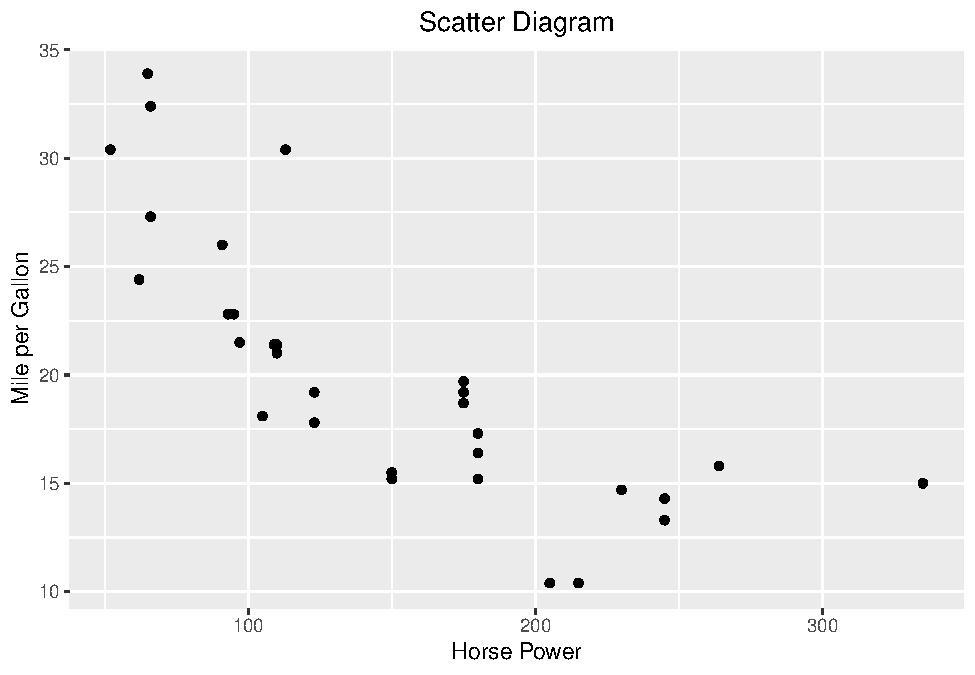
\includegraphics{bailey_files/figure-latex/unnamed-chunk-78-1.pdf}

It appears as if mpg falls at a diminishing rate as horse power increases. There are a number of functional forms that will gives us that basic shape. One such form is quadratic. Let's estimate a quadratic form of the model \(mpg = \beta_0+\beta_1hp+\beta_2hp+\epsilon\)

\begin{Shaded}
\begin{Highlighting}[]
\NormalTok{mtcars }\OperatorTok\StringTok{ }
\StringTok{  }\KeywordTok{lm}\NormalTok{(mpg }\OperatorTok{~}\StringTok{ }\NormalTok{hp }\OperatorTok{+}\StringTok{ }\KeywordTok{I}\NormalTok{(hp}\OperatorTok{^}\DecValTok{2}\NormalTok{)) }\CommentTok{# uses the AsIs function I() to create hp squared}
\end{Highlighting}
\end{Shaded}

\begin{verbatim}

Call:
lm(formula = mpg ~ hp + I(hp^2))

Coefficients:
(Intercept)           hp      I(hp^2)  
  40.409117    -0.213308     0.000421  
\end{verbatim}

Add the quadratic fit to the scatter diagram

\begin{Shaded}
\begin{Highlighting}[]
\NormalTok{p }\OperatorTok{+}\StringTok{ }
\StringTok{  }\KeywordTok{geom_smooth}\NormalTok{(}\DataTypeTok{method =} \StringTok{"lm"}\NormalTok{, }\DataTypeTok{formula =}\NormalTok{ y }\OperatorTok{~}\StringTok{  }\NormalTok{x }\OperatorTok{+}\StringTok{ }\KeywordTok{I}\NormalTok{(x}\OperatorTok{^}\DecValTok{2}\NormalTok{), }\DataTypeTok{se =}\NormalTok{ F)}
\end{Highlighting}
\end{Shaded}

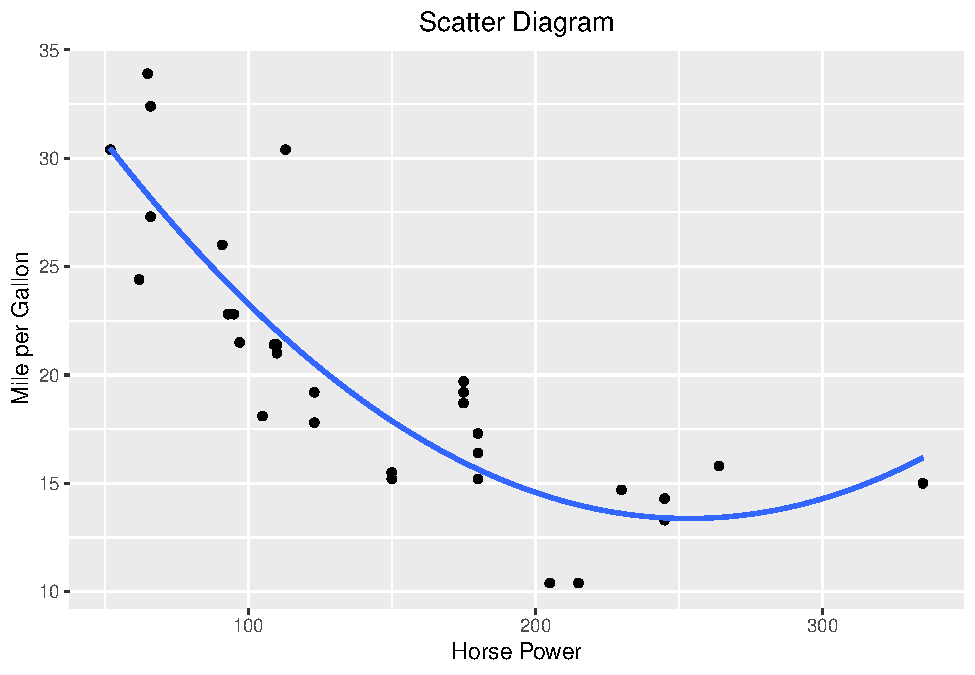
\includegraphics{bailey_files/figure-latex/unnamed-chunk-80-1.pdf}

Adding higher order polynomials is accomplished by adding additional AsIs functions \texttt{I()} to the model.

\hypertarget{logarithmic}{%
\section{Logarithmic}\label{logarithmic}}

Logarithms have a wide variety of uses in Econometrics.

\hypertarget{constant-elasticity-log-log-or-double-log}{%
\subsection{Constant Elasticity (log-log or double log)}\label{constant-elasticity-log-log-or-double-log}}

Log-log models are of the form \(\ln y = \beta_0 + \beta_1\ln x\). So \(\beta_1 = \frac{d\ln y}{d\ln x}\)

Recall that \(dlnX=\frac{dX}{X}\); that is, the change in the logarithm is a percent change in a variable. For example, \(\Delta lnP\) is the \% change in \(P\).

So, \(\beta_1\) is the percent change in y resultant from a 1\% change in x. Or, a one \emph{percent} change in x will induce a \(\beta_1\) \emph{percent} change in y.

Constant elasticity demand functions are estimated using log-log models. Let, \(q=\alpha p^\beta\) where \(\beta<0\) be the demand function. Recall he elasticity of demand is given by \(\eta=\frac{\%\Delta q}{\%\Delta p} = \frac{dq/q}{dp/p}=\frac{dq}{dp}\frac{p}{q}\). The elasticity of demand for our demand function is \[\eta=\beta\alpha p^{\beta-1}\frac{p}{q}=\frac{\beta\alpha p^{\beta}}{q}\] Substitute for \(q=\alpha p^\beta\) \[\eta=\frac{\beta\alpha p^{\beta}}{\alpha p^\beta}=\beta\] The elasticity of demand is \(\beta\) which is invariant. To make \(q=\alpha p^\beta\) estimable with OLS take the logarithm of both sides: \[\ln(q)=\ln(\alpha p^\beta\epsilon)\] \[\ln(q)=\ln(\alpha)+\ln( p^\beta)+\ln(\epsilon)\] \[\ln(q)=\gamma+\beta\ln(p) + \delta\] is now in estimable form and can estimated by \texttt{lm(log(q)\ \textasciitilde{}\ log(p),\ data\ =\ df)}

Cobb-Douglas production functions are also estimated as log-log models. Let's estimate a Cobb-Douglas model for horsepower as a function of number of cylinders and displacement in cubic inches from the mtcars data. The production function is: \[hp=\beta_0cyl^{\beta_1}disp^{\beta_2}\epsilon\] The estimable form of the model is \[\ln hp=\alpha_0+\beta_1\ln cyl+\beta_2\ln disp+\gamma\]

\begin{Shaded}
\begin{Highlighting}[]
\NormalTok{mtcars }\OperatorTok
\StringTok{  }\KeywordTok{lm}\NormalTok{(}\KeywordTok{log}\NormalTok{(hp) }\OperatorTok{~}\StringTok{ }\KeywordTok{log}\NormalTok{(cyl) }\OperatorTok{+}\StringTok{ }\KeywordTok{log}\NormalTok{(disp))}
\end{Highlighting}
\end{Shaded}

\begin{verbatim}

Call:
lm(formula = log(hp) ~ log(cyl) + log(disp))

Coefficients:
(Intercept)     log(cyl)    log(disp)  
      1.851        0.817        0.299  
\end{verbatim}

\(\hat\beta_1\) indicates that a 1\% increase in the number of cylinders, \emph{ceteris paribus}, increases horsepower by 0.8170\%. \(\hat\beta_2\) indicates that a 1\% increase in the displacement, \emph{ceteris paribus} increases horsepower by 0.2986\%.

\hypertarget{constant-growth-in-a-dependent-variable-log-lin-or-semilog}{%
\subsection{Constant Growth in a Dependent Variable (log-lin or semilog)}\label{constant-growth-in-a-dependent-variable-log-lin-or-semilog}}

The log-lin model has the form \(\ln y = \beta_0 + \beta_1x\). \(\beta_1 = \frac{d\ln y}{dx}\) or the percent change in y resultant from a 1 unit change in x. Or, a \emph{unit} change in x will induce a \(100*\beta_1\) \emph{percent} change in y.

Suppose we have a variable P that is growing at a constant rate of g per period t such that \(P_t=(1+g)P_{t-1}\). By repeated substitution we get \(P_t=P_0(1+g)^t\) where \(P_0\) is the initial value of Y. \^{}{[}Note the relationship to the time value of money. Let \(FV=PV(1+r)^t\). Suppose we'd like to calculate the average annual rate of return, r, on \(\$PV\), given a future value of \(\$FV\). After appropriate algebraic gymnastics, \[r = \sqrt[t] { \frac{FV}{PV} } - 1\]. We could calculate g without regression as \[g=\sqrt[t]{ \frac{P_t}{P_0} }-1\]. We could calculate g with a regression with the aid of logarithms. Let the model be \(P_t=P_0(1+g)^t\epsilon\). Taking the logarithm of both sides yields \[\ln(P_t)=\ln(P_0)+t\ln(1+g)+\ln(\epsilon)\] Which we can estimate as \[Y_t=\beta_0+\beta_1t+u_t\] Where \(\beta_0=\ln(P_0)\), \(u_t = \ln(\epsilon_t)\), and, most importantly, \(\beta_1=\ln(1+g)\). We can get our estimate of \(g\) from \(\hat\beta_1=\widehat{\ln(1+g)}\) by exponentiating both sides and solving for \(g\). \[e^{\hat\beta_1}=e^{\widehat{\ln(1+g)}}\] \[\hat{g}=e^{\hat\beta_1}-1\] \footnote{We know that \(\beta_1=\frac{d(\ln P_t)}{dt}\). Since \(d(\ln P_t)=\frac{dP_t}{P_t}\) or the percent change in \(P_t\), \(\beta_1\) is known as the \textbf{instantaneous rate of growth}.}

Suppose we'd like to know the percent change in fuel mileage resultant from adding a cylinder to the car using the mtcars data. Estimate the model \(\ln mpg=\beta_0+\beta_1cyl+\epsilon\)

\begin{Shaded}
\begin{Highlighting}[]
\NormalTok{mtcars }\OperatorTok\StringTok{ }
\StringTok{  }\KeywordTok{lm}\NormalTok{(}\KeywordTok{log}\NormalTok{(mpg) }\OperatorTok{~}\StringTok{ }\NormalTok{cyl)}
\end{Highlighting}
\end{Shaded}

\begin{verbatim}

Call:
lm(formula = log(mpg) ~ cyl)

Coefficients:
(Intercept)          cyl  
      3.839       -0.143  
\end{verbatim}

\(\hat\beta_1\) indicates that adding one cylinder reduces fuel mileage by 14.25\%.

\hypertarget{constant-change-in-dependent-variable-lin-log}{%
\subsection{Constant \% Change in Dependent Variable (lin-log)}\label{constant-change-in-dependent-variable-lin-log}}

The lin-log model has the form \(y=\beta_0+\beta_1\ln x\). \(\beta_1 = \frac{dy}{d\ln x}\) or the change in y from a 1 percent change in x. Or, one \emph{percent} change in x will induce a \(\frac{\beta_1}{100}\) \emph{unit} change in y.

Suppose we'd like to know the change in the number of miles per gallon as a function of the percent change in displacement. Estimate the model \(mpg=\beta_0+beta_1\ln disp+\epsilon\)

\begin{Shaded}
\begin{Highlighting}[]
\NormalTok{mtcars }\OperatorTok
\StringTok{  }\KeywordTok{lm}\NormalTok{(mpg }\OperatorTok{~}\StringTok{ }\KeywordTok{log}\NormalTok{(disp))}
\end{Highlighting}
\end{Shaded}

\begin{verbatim}

Call:
lm(formula = mpg ~ log(disp))

Coefficients:
(Intercept)    log(disp)  
      69.21        -9.29  
\end{verbatim}

\(\hat\beta_1\) indicates that a one percent change in displacement will decrease fuel mileage by .093 mpg.

\hypertarget{other-useful-functional-forms}{%
\section{Other Useful Functional Forms}\label{other-useful-functional-forms}}

We know that marginal analysis is the \emph{sine qua non} of economic reasoning. So our economic models should be built with an eye toward what we think the marginal relationship should look like from theory. Use a sort ``a poor man's'' differential equations to work from a marginal model to the functional form. For example, consider production as a function of labor holding capital constant \(Q=Q(\bar K, L)\) with K fixed at \(\bar K\). From microeconomic theory we know that the marginal product of labor, \(MP_L=\frac{dQ}{dl}\) at some point diminishes. This suggests \(MP_L=\beta_1+\beta_2L+\beta_3L^2\) where \(\beta_1\ge0, \beta_2>0, \text{ and } \beta_3<0\) as the model product of labor. The production function that will yield this marginal product is \(Q=\beta_0+\beta_1L+\beta_2L^2+\beta_3L^3\). Thus the usefulness of a polynomial functional form in economics.

There are other functional forms that will yield diminishing marginal functions. For example, another functional form that will yield a diminishing marginal is a rectangular hyperbola \(y=\beta_0+\frac{\beta_1}{x}\). The marginal effect of x on y is \(\frac{dy}{dx}=\frac{-\beta_1}{x^2}\). A one unit change in X leads to a \(\frac{1}{x}\) change in y. Notice as x increases the change in y decreases, i.e., diminishing marginal.

The plot of miles per gallon vs.~horsepower above suggests a negative diminishing relationship between the variables. Suppose we postulate that miles per gallon is a function of the inverse of horsepower \(mpg = \beta_0 + \frac{\beta_1}{hp}+\epsilon\).

\begin{Shaded}
\begin{Highlighting}[]
\NormalTok{mtcars }\OperatorTok
\StringTok{  }\KeywordTok{lm}\NormalTok{(mpg }\OperatorTok{~}\StringTok{ }\KeywordTok{I}\NormalTok{(}\DecValTok{1}\OperatorTok{/}\NormalTok{hp))}
\end{Highlighting}
\end{Shaded}

\begin{verbatim}

Call:
lm(formula = mpg ~ I(1/hp))

Coefficients:
(Intercept)      I(1/hp)  
       9.43      1259.88  
\end{verbatim}

Add the fitted model to scatter diagram.

\begin{Shaded}
\begin{Highlighting}[]
\NormalTok{p }\OperatorTok{+}\StringTok{ }
\StringTok{  }\KeywordTok{geom_smooth}\NormalTok{(}\DataTypeTok{method =}\NormalTok{ lm, }\DataTypeTok{formula =}\NormalTok{ y }\OperatorTok{~}\StringTok{ }\KeywordTok{I}\NormalTok{(}\DecValTok{1}\OperatorTok{/}\NormalTok{x), }\DataTypeTok{se =}\NormalTok{ F)}
\end{Highlighting}
\end{Shaded}

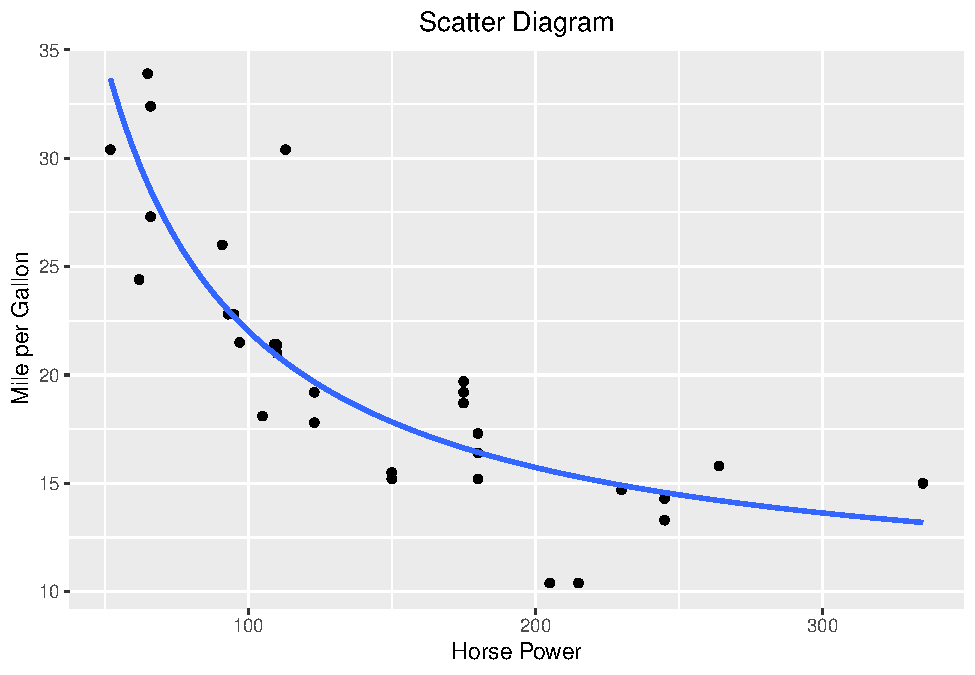
\includegraphics{bailey_files/figure-latex/unnamed-chunk-85-1.pdf}

\hypertarget{chp8}{%
\chapter{Using Fixed Effects Models to Fight Endogeneity in Panel Data and Difference--in--Difference Models}\label{chp8}}

In this chapter we will learn to deal with panel data in R. Panel data are data that include observations in and through time. Panel data combine aspects of cross--sectional data with time--series data. The libraries necessary for this chapter are:

\begin{Shaded}
\begin{Highlighting}[]
\KeywordTok{library}\NormalTok{(tidyverse)}
\KeywordTok{library}\NormalTok{(magrittr)}
\KeywordTok{library}\NormalTok{(broom)}
\KeywordTok{library}\NormalTok{(estimatr)}
\KeywordTok{library}\NormalTok{(carData)}
\end{Highlighting}
\end{Shaded}

\hypertarget{simpsons-paradox}{%
\section{Simpson's Paradox}\label{simpsons-paradox}}

Simpson's paradox - Simpson (\href{https://www.jstor.org/stable/2984065?seq=1\#metadata_info_tab_contents}{1951}) is phenomenon where an apparent relationship between two variables reverses itself when the data are dis-aggregated. For example, let's look at the admissions rate for men and women in the University of California at Berkeley admissions data.

UCBAdmissions is a cross-tabulation of 4526 applicants by 3 variables: Admit, Gender, and Dept, the number of observations for each is n stored as 3-dimensional array.

\begin{Shaded}
\begin{Highlighting}[]
\NormalTok{UCBAdmissions}
\end{Highlighting}
\end{Shaded}

\begin{verbatim}
, , Dept = A

          Gender
Admit      Male Female
  Admitted  512     89
  Rejected  313     19

, , Dept = B

          Gender
Admit      Male Female
  Admitted  353     17
  Rejected  207      8

, , Dept = C

          Gender
Admit      Male Female
  Admitted  120    202
  Rejected  205    391

, , Dept = D

          Gender
Admit      Male Female
  Admitted  138    131
  Rejected  279    244

, , Dept = E

          Gender
Admit      Male Female
  Admitted   53     94
  Rejected  138    299

, , Dept = F

          Gender
Admit      Male Female
  Admitted   22     24
  Rejected  351    317
\end{verbatim}

To calculate admission rates, we need to create a new variable, apps, that is the sum of admitted and rejected apps for both men and women.

\begin{Shaded}
\begin{Highlighting}[]
\NormalTok{UCBAdmissions }\OperatorTok\StringTok{ }
\StringTok{  }\KeywordTok{as_tibble}\NormalTok{() }\OperatorTok\StringTok{ }\CommentTok{# convert the table to a data frame}
\StringTok{  }\KeywordTok{group_by}\NormalTok{(Dept, Gender) }\OperatorTok\StringTok{  }\CommentTok{# allows us to sum admitted and rejected by department}
\StringTok{  }\KeywordTok{mutate}\NormalTok{(}\DataTypeTok{apps =} \KeywordTok{sum}\NormalTok{(n)) }\OperatorTok\StringTok{ }\CommentTok{# create number of applicants by department}
\StringTok{  }\KeywordTok{ungroup}\NormalTok{() }\OperatorTok\StringTok{ }\CommentTok{# return the full data frame}
\StringTok{  }\KeywordTok{filter}\NormalTok{(Admit }\OperatorTok{==}\StringTok{ "Admitted"}\NormalTok{) }\OperatorTok\StringTok{ }\CommentTok{# select only those applicants admitted}
\StringTok{  }\KeywordTok{group_by}\NormalTok{(Gender) }\OperatorTok\StringTok{ }\CommentTok{# allows us to calculate acceptance rates by gender}
\StringTok{  }\KeywordTok{summarize}\NormalTok{(}\DataTypeTok{rate =} \KeywordTok{sum}\NormalTok{(n)}\OperatorTok{/}\KeywordTok{sum}\NormalTok{(apps))}
\end{Highlighting}
\end{Shaded}

\begin{verbatim}
# A tibble: 2 x 2
  Gender  rate
  <chr>  <dbl>
1 Female 0.304
2 Male   0.445
\end{verbatim}

Males are accepted at rate of 44.5\% while females are accepted at lower rate of 30.4\%.

\begin{Shaded}
\begin{Highlighting}[]
\NormalTok{UCBAdmissions }\OperatorTok\StringTok{ }
\StringTok{  }\KeywordTok{as_tibble}\NormalTok{() }\OperatorTok\StringTok{ }
\StringTok{  }\KeywordTok{group_by}\NormalTok{(Dept, Gender) }\OperatorTok\StringTok{  }
\StringTok{  }\KeywordTok{mutate}\NormalTok{(}\DataTypeTok{apps =} \KeywordTok{sum}\NormalTok{(n)) }\OperatorTok\StringTok{ }
\StringTok{  }\KeywordTok{ungroup}\NormalTok{() }\OperatorTok\StringTok{ }
\StringTok{  }\KeywordTok{filter}\NormalTok{(Admit }\OperatorTok{==}\StringTok{ "Admitted"}\NormalTok{) }\OperatorTok\StringTok{ }
\StringTok{  }\KeywordTok{group_by}\NormalTok{(Dept, Gender) }\OperatorTok\StringTok{ }
\StringTok{  }\KeywordTok{summarize}\NormalTok{(n}\OperatorTok{/}\NormalTok{apps)}
\end{Highlighting}
\end{Shaded}

\begin{verbatim}
# A tibble: 12 x 3
# Groups:   Dept [6]
   Dept  Gender `n/apps`
   <chr> <chr>     <dbl>
 1 A     Female   0.824 
 2 A     Male     0.621 
 3 B     Female   0.68  
 4 B     Male     0.630 
 5 C     Female   0.341 
 6 C     Male     0.369 
 7 D     Female   0.349 
 8 D     Male     0.331 
 9 E     Female   0.239 
10 E     Male     0.277 
11 F     Female   0.0704
12 F     Male     0.0590
\end{verbatim}

We now see that females are admitted at higher rates to four of the six departments.

\hypertarget{figures-8.1-8.3}{%
\section{Figures 8.1-8.3}\label{figures-8.1-8.3}}

We see a similar effect in Figures 8.1-8.3 in the text. We can reproduce those graphs with the code below. The crime data set contains observations on 19 variables from 58 cities over the period 1972 to 1993. First choose observations for only the California cities of Fresno, Los Angeles, Oakland, Sacramento, and San Francisco. Next convert the robbery and police to numbers per 1000 persons. The data frame crime contains the data.\# the \%in\% operator means match the elements in one vector with elements in another.

\begin{Shaded}
\begin{Highlighting}[]
\NormalTok{crime }\OperatorTok\StringTok{ }
\StringTok{  }\KeywordTok{select}\NormalTok{(cityname, policesworn, robbery, popcity) }\OperatorTok\StringTok{ }\CommentTok{# choose relevant variables}
\StringTok{  }\KeywordTok{filter}\NormalTok{(cityname }\OperatorTok\StringTok{ }\KeywordTok{c}\NormalTok{(}\StringTok{"fresno"}\NormalTok{, }\StringTok{"losangel"}\NormalTok{, }\StringTok{"oakland"}\NormalTok{, }\StringTok{"sacramen"}\NormalTok{, }\StringTok{"sanfran"}\NormalTok{)) }\OperatorTok\StringTok{ }\CommentTok{# choose relevant cities}
\StringTok{  }\KeywordTok{mutate}\NormalTok{(}\DataTypeTok{robbery=}\NormalTok{robbery}\OperatorTok{/}\NormalTok{popcity}\OperatorTok{*}\DecValTok{1000}\NormalTok{, }\DataTypeTok{policesworn =}\NormalTok{ policesworn}\OperatorTok{/}\NormalTok{popcity}\OperatorTok{*}\DecValTok{1000}\NormalTok{) }\OperatorTok\StringTok{ }\CommentTok{# convert to per 1000}
\StringTok{  }\KeywordTok{ggplot}\NormalTok{(}\KeywordTok{aes}\NormalTok{(}\DataTypeTok{x =}\NormalTok{ policesworn, }\DataTypeTok{y =}\NormalTok{ robbery)) }\OperatorTok{+}
\StringTok{  }\KeywordTok{geom_point}\NormalTok{(}\DataTypeTok{na.rm =}\NormalTok{ T) }\OperatorTok{+}\StringTok{ }
\StringTok{  }\KeywordTok{geom_smooth}\NormalTok{(}\DataTypeTok{method =}\NormalTok{ lm, }\DataTypeTok{na.rm =}\NormalTok{ T, }\DataTypeTok{se =}\NormalTok{ F) }\OperatorTok{+}\StringTok{ }
\StringTok{  }\KeywordTok{xlab}\NormalTok{(}\StringTok{"Police per 1000 People"}\NormalTok{) }\OperatorTok{+}\StringTok{ }
\StringTok{  }\KeywordTok{ylab}\NormalTok{(}\StringTok{"Robberies per 1000 People"}\NormalTok{) }\OperatorTok{+}
\StringTok{  }\KeywordTok{labs}\NormalTok{(}\DataTypeTok{caption =} \StringTok{"Figure 8.1: Robberies and Police for Large Cities in California"}\NormalTok{) }\OperatorTok{+}\StringTok{ }\CommentTok{# create caption}
\StringTok{  }\KeywordTok{theme}\NormalTok{(}\DataTypeTok{plot.caption =} \KeywordTok{element_text}\NormalTok{(}\DataTypeTok{hjust =} \DecValTok{0}\NormalTok{)) }\CommentTok{# left justify the caption}
\end{Highlighting}
\end{Shaded}

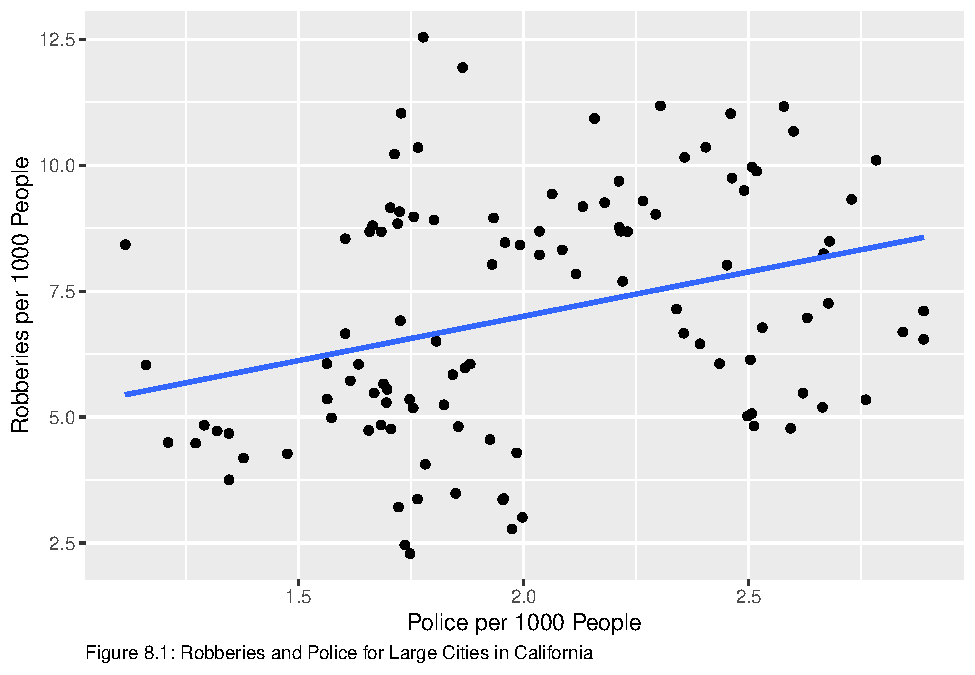
\includegraphics{bailey_files/figure-latex/figure8.1-1.pdf}

\begin{Shaded}
\begin{Highlighting}[]
\NormalTok{crime }\OperatorTok\StringTok{ }
\StringTok{  }\KeywordTok{select}\NormalTok{(cityname, policesworn, robbery, popcity) }\OperatorTok\StringTok{ }
\StringTok{  }\KeywordTok{filter}\NormalTok{(cityname }\OperatorTok\StringTok{ }\KeywordTok{c}\NormalTok{(}\StringTok{"fresno"}\NormalTok{, }\StringTok{"losangel"}\NormalTok{, }\StringTok{"oakland"}\NormalTok{, }\StringTok{"sacramen"}\NormalTok{, }\StringTok{"sanfran"}\NormalTok{)) }\OperatorTok\StringTok{ }
\StringTok{  }\KeywordTok{mutate}\NormalTok{(}\DataTypeTok{robbery=}\NormalTok{robbery}\OperatorTok{/}\NormalTok{popcity}\OperatorTok{*}\DecValTok{1000}\NormalTok{, }\DataTypeTok{policesworn =}\NormalTok{ policesworn}\OperatorTok{/}\NormalTok{popcity}\OperatorTok{*}\DecValTok{1000}\NormalTok{) }\OperatorTok\StringTok{ }
\StringTok{  }\KeywordTok{ggplot}\NormalTok{(}\KeywordTok{aes}\NormalTok{(}\DataTypeTok{x =}\NormalTok{ policesworn, }\DataTypeTok{y =}\NormalTok{ robbery, }\DataTypeTok{color =}\NormalTok{ cityname)) }\OperatorTok{+}
\StringTok{  }\KeywordTok{geom_point}\NormalTok{(}\DataTypeTok{na.rm =}\NormalTok{ T) }\OperatorTok{+}\StringTok{ }
\StringTok{  }\KeywordTok{xlab}\NormalTok{(}\StringTok{"Police per 1000 People"}\NormalTok{) }\OperatorTok{+}\StringTok{ }
\StringTok{  }\KeywordTok{ylab}\NormalTok{(}\StringTok{"Robberies per 1000 People"}\NormalTok{) }\OperatorTok{+}
\StringTok{  }\KeywordTok{labs}\NormalTok{(}\DataTypeTok{caption =} \StringTok{"Figure 8.2: Robberies and Police for Specified Cities in California"}\NormalTok{) }\OperatorTok{+}\StringTok{ }
\StringTok{  }\KeywordTok{theme}\NormalTok{(}\DataTypeTok{plot.caption =} \KeywordTok{element_text}\NormalTok{(}\DataTypeTok{hjust =} \DecValTok{0}\NormalTok{), }\DataTypeTok{legend.position =} \StringTok{"none"}\NormalTok{) }\OperatorTok{+}\StringTok{ }\CommentTok{# remove legend}
\StringTok{  }\CommentTok{# place city names with corresponding colors.}
\StringTok{  }\KeywordTok{annotate}\NormalTok{(}\DataTypeTok{geom =} \StringTok{"text"}\NormalTok{, }\DataTypeTok{x =} \FloatTok{1.6}\NormalTok{, }\DataTypeTok{y =} \DecValTok{10}\NormalTok{, }\DataTypeTok{label =} \StringTok{"Oakland"}\NormalTok{, }\DataTypeTok{col =} \StringTok{"#00BF7D"}\NormalTok{) }\OperatorTok{+}\StringTok{ }
\StringTok{  }\KeywordTok{annotate}\NormalTok{(}\DataTypeTok{geom =} \StringTok{"text"}\NormalTok{, }\DataTypeTok{x =} \DecValTok{2}\NormalTok{, }\DataTypeTok{y =} \DecValTok{5}\NormalTok{, }\DataTypeTok{label =} \StringTok{"Sacramento"}\NormalTok{, }\DataTypeTok{col =} \StringTok{"#00B0F6"}\NormalTok{) }\OperatorTok{+}\StringTok{ }
\StringTok{  }\KeywordTok{annotate}\NormalTok{(}\DataTypeTok{geom =} \StringTok{"text"}\NormalTok{, }\DataTypeTok{x =} \FloatTok{2.58}\NormalTok{, }\DataTypeTok{y =} \FloatTok{4.5}\NormalTok{, }\DataTypeTok{label =} \StringTok{"Los Angeles"}\NormalTok{, }\DataTypeTok{col =} \StringTok{"#A3A500"}\NormalTok{) }\OperatorTok{+}\StringTok{ }
\StringTok{  }\KeywordTok{annotate}\NormalTok{(}\DataTypeTok{geom =} \StringTok{"text"}\NormalTok{, }\DataTypeTok{x =} \FloatTok{2.7}\NormalTok{, }\DataTypeTok{y =} \FloatTok{7.8}\NormalTok{, }\DataTypeTok{label =} \StringTok{"San Francisco"}\NormalTok{, }\DataTypeTok{col =} \StringTok{"#E76BF3"}\NormalTok{) }\OperatorTok{+}\StringTok{ }
\StringTok{  }\KeywordTok{annotate}\NormalTok{(}\DataTypeTok{geom =} \StringTok{"text"}\NormalTok{, }\DataTypeTok{x =} \FloatTok{1.25}\NormalTok{, }\DataTypeTok{y =} \FloatTok{3.5}\NormalTok{, }\DataTypeTok{label =} \StringTok{"Fresno"}\NormalTok{, }\DataTypeTok{col =} \StringTok{"#F8766D"}\NormalTok{)}
\end{Highlighting}
\end{Shaded}

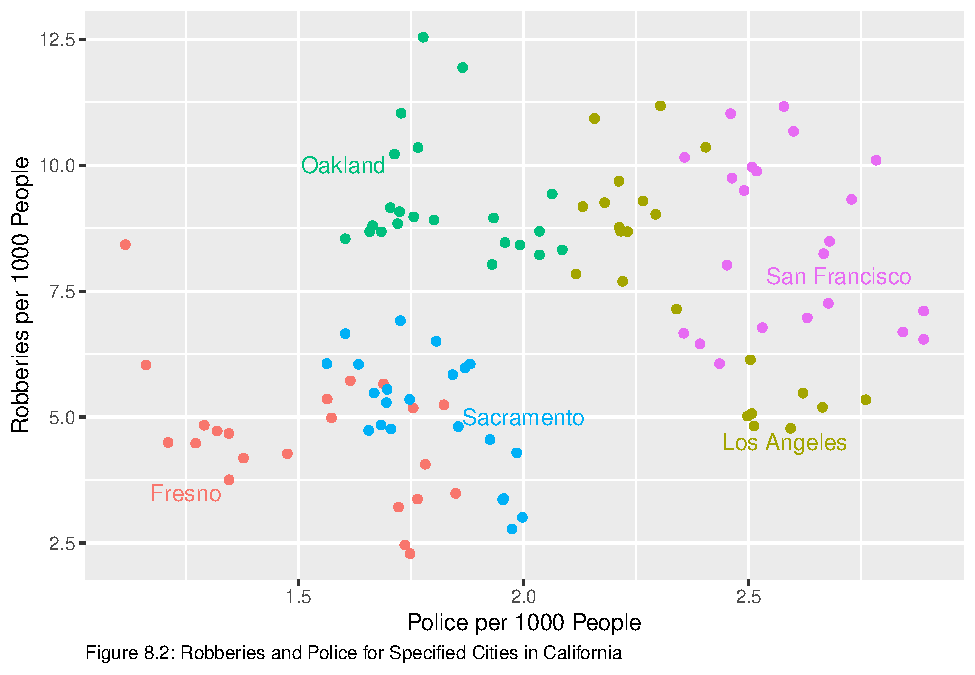
\includegraphics{bailey_files/figure-latex/figure8.2-1.pdf}

\begin{Shaded}
\begin{Highlighting}[]
\NormalTok{crime }\OperatorTok\StringTok{ }
\StringTok{  }\KeywordTok{select}\NormalTok{(cityname, policesworn, robbery, popcity) }\OperatorTok\StringTok{ }
\StringTok{  }\KeywordTok{filter}\NormalTok{(cityname }\OperatorTok\StringTok{ }\KeywordTok{c}\NormalTok{(}\StringTok{"fresno"}\NormalTok{, }\StringTok{"losangel"}\NormalTok{, }\StringTok{"oakland"}\NormalTok{, }\StringTok{"sacramen"}\NormalTok{, }\StringTok{"sanfran"}\NormalTok{)) }\OperatorTok\StringTok{ }
\StringTok{  }\KeywordTok{mutate}\NormalTok{(}\DataTypeTok{robbery=}\NormalTok{robbery}\OperatorTok{/}\NormalTok{popcity}\OperatorTok{*}\DecValTok{1000}\NormalTok{, }\DataTypeTok{policesworn =}\NormalTok{ policesworn}\OperatorTok{/}\NormalTok{popcity}\OperatorTok{*}\DecValTok{1000}\NormalTok{) }\OperatorTok\StringTok{ }
\StringTok{  }\KeywordTok{ggplot}\NormalTok{(}\KeywordTok{aes}\NormalTok{(}\DataTypeTok{x =}\NormalTok{ policesworn, }\DataTypeTok{y =}\NormalTok{ robbery, }\DataTypeTok{color =}\NormalTok{ cityname)) }\OperatorTok{+}
\StringTok{  }\KeywordTok{geom_point}\NormalTok{(}\DataTypeTok{na.rm =}\NormalTok{ T) }\OperatorTok{+}\StringTok{ }
\StringTok{  }\KeywordTok{xlab}\NormalTok{(}\StringTok{"Police per 1000 People"}\NormalTok{) }\OperatorTok{+}\StringTok{ }
\StringTok{  }\KeywordTok{ylab}\NormalTok{(}\StringTok{"Robberies per 1000 People"}\NormalTok{) }\OperatorTok{+}
\StringTok{  }\KeywordTok{labs}\NormalTok{(}\DataTypeTok{caption =} \StringTok{"Figure 8.3: Robberies and Police for Specified Cities in California with City-Specific Regression Lines"}\NormalTok{) }\OperatorTok{+}\StringTok{ }
\StringTok{  }\KeywordTok{theme}\NormalTok{(}\DataTypeTok{plot.caption =} \KeywordTok{element_text}\NormalTok{(}\DataTypeTok{hjust =} \DecValTok{0}\NormalTok{), }\DataTypeTok{legend.position =} \StringTok{"none"}\NormalTok{) }\OperatorTok{+}\StringTok{ }
\StringTok{  }\KeywordTok{annotate}\NormalTok{(}\DataTypeTok{geom =} \StringTok{"text"}\NormalTok{, }\DataTypeTok{x =} \FloatTok{1.6}\NormalTok{, }\DataTypeTok{y =} \DecValTok{10}\NormalTok{, }\DataTypeTok{label =} \StringTok{"Oakland"}\NormalTok{, }\DataTypeTok{col =} \StringTok{"#00BF7D"}\NormalTok{) }\OperatorTok{+}\StringTok{ }
\StringTok{  }\KeywordTok{annotate}\NormalTok{(}\DataTypeTok{geom =} \StringTok{"text"}\NormalTok{, }\DataTypeTok{x =} \DecValTok{2}\NormalTok{, }\DataTypeTok{y =} \DecValTok{5}\NormalTok{, }\DataTypeTok{label =} \StringTok{"Sacramento"}\NormalTok{, }\DataTypeTok{col =} \StringTok{"#00B0F6"}\NormalTok{) }\OperatorTok{+}\StringTok{ }
\StringTok{  }\KeywordTok{annotate}\NormalTok{(}\DataTypeTok{geom =} \StringTok{"text"}\NormalTok{, }\DataTypeTok{x =} \FloatTok{2.58}\NormalTok{, }\DataTypeTok{y =} \FloatTok{4.5}\NormalTok{, }\DataTypeTok{label =} \StringTok{"Los Angeles"}\NormalTok{, }\DataTypeTok{col =} \StringTok{"#A3A500"}\NormalTok{) }\OperatorTok{+}\StringTok{ }
\StringTok{  }\KeywordTok{annotate}\NormalTok{(}\DataTypeTok{geom =} \StringTok{"text"}\NormalTok{, }\DataTypeTok{x =} \FloatTok{2.7}\NormalTok{, }\DataTypeTok{y =} \FloatTok{7.8}\NormalTok{, }\DataTypeTok{label =} \StringTok{"San Francisco"}\NormalTok{, }\DataTypeTok{col =} \StringTok{"#E76BF3"}\NormalTok{) }\OperatorTok{+}\StringTok{ }
\StringTok{  }\KeywordTok{annotate}\NormalTok{(}\DataTypeTok{geom =} \StringTok{"text"}\NormalTok{, }\DataTypeTok{x =} \FloatTok{1.25}\NormalTok{, }\DataTypeTok{y =} \FloatTok{3.5}\NormalTok{, }\DataTypeTok{label =} \StringTok{"Fresno"}\NormalTok{, }\DataTypeTok{col =} \StringTok{"#F8766D"}\NormalTok{) }\OperatorTok{+}
\StringTok{  }\KeywordTok{geom_smooth}\NormalTok{(}\DataTypeTok{method =} \StringTok{"lm"}\NormalTok{, }\DataTypeTok{se =}\NormalTok{ F) }\CommentTok{# add regression lines. the addition of the color aesthetic will cause geom_smooth to add regression lines for each "color"}
\end{Highlighting}
\end{Shaded}

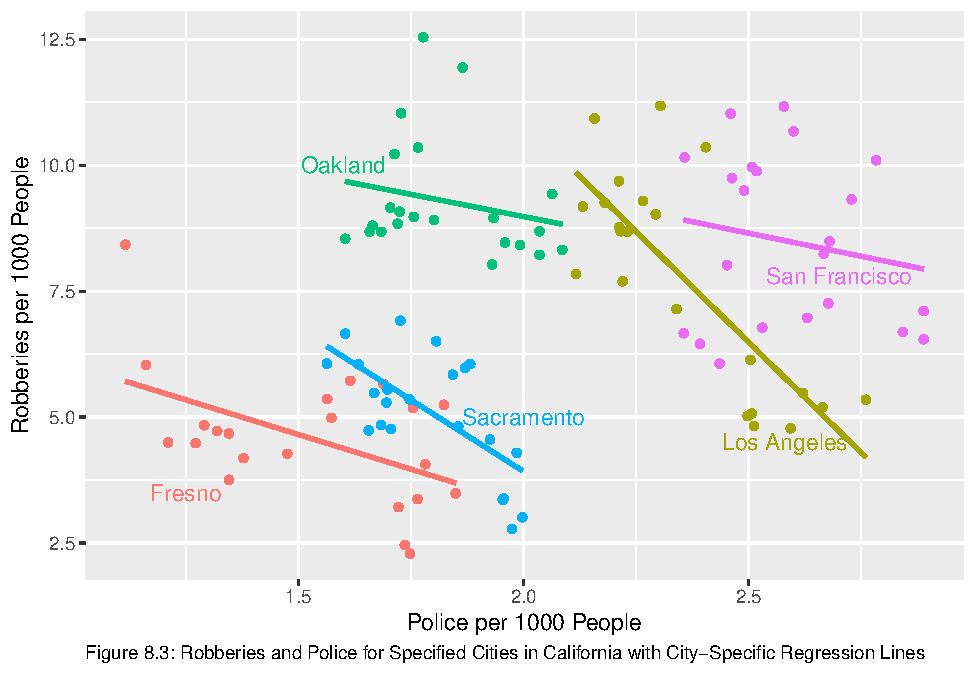
\includegraphics{bailey_files/figure-latex/figure8.3-1.pdf}

\hypertarget{one-way-fixed-effects-models}{%
\section{One-Way Fixed Effects Models}\label{one-way-fixed-effects-models}}

\hypertarget{lsdv-approach}{%
\subsection{LSDV Approach}\label{lsdv-approach}}

The least squares dummy variable approach allows us to account for the fixed effects by including a dummy variable for each unit. First, let's calculate the pooled model.

\begin{Shaded}
\begin{Highlighting}[]
\NormalTok{crime }\OperatorTok\StringTok{ }
\StringTok{  }\KeywordTok{select}\NormalTok{(cityname, policesworn, robbery, popcity) }\OperatorTok\StringTok{ }
\StringTok{  }\KeywordTok{filter}\NormalTok{(cityname }\OperatorTok\StringTok{ }\KeywordTok{c}\NormalTok{(}\StringTok{"fresno"}\NormalTok{, }\StringTok{"losangel"}\NormalTok{, }\StringTok{"oakland"}\NormalTok{, }\StringTok{"sacramen"}\NormalTok{, }\StringTok{"sanfran"}\NormalTok{)) }\OperatorTok\StringTok{ }
\StringTok{  }\KeywordTok{mutate}\NormalTok{(}\DataTypeTok{robbery=}\NormalTok{robbery}\OperatorTok{/}\NormalTok{popcity}\OperatorTok{*}\DecValTok{1000}\NormalTok{, }\DataTypeTok{policesworn =}\NormalTok{ policesworn}\OperatorTok{/}\NormalTok{popcity}\OperatorTok{*}\DecValTok{1000}\NormalTok{) }\OperatorTok
\StringTok{  }\KeywordTok{lm}\NormalTok{(robbery }\OperatorTok{~}\StringTok{ }\NormalTok{policesworn) }\OperatorTok\StringTok{ }
\StringTok{  }\KeywordTok{tidy}\NormalTok{()}
\end{Highlighting}
\end{Shaded}

\begin{verbatim}
# A tibble: 2 x 5
  term        estimate std.error statistic  p.value
  <chr>          <dbl>     <dbl>     <dbl>    <dbl>
1 (Intercept)     3.48     1.05       3.31 0.00129 
2 policesworn     1.76     0.509      3.46 0.000771
\end{verbatim}

We can see that the coefficient on the police variable is positive and significantly different than zero.

To apply LSDV approach in R, we add cityname as an explanatory variable. Since cityname is a character vector, R will treat it as a factor.

\begin{Shaded}
\begin{Highlighting}[]
\NormalTok{crime }\OperatorTok\StringTok{ }
\StringTok{  }\KeywordTok{select}\NormalTok{(cityname, policesworn, robbery, popcity) }\OperatorTok\StringTok{ }
\StringTok{  }\KeywordTok{filter}\NormalTok{(cityname }\OperatorTok\StringTok{ }\KeywordTok{c}\NormalTok{(}\StringTok{"fresno"}\NormalTok{, }\StringTok{"losangel"}\NormalTok{, }\StringTok{"oakland"}\NormalTok{, }\StringTok{"sacramen"}\NormalTok{, }\StringTok{"sanfran"}\NormalTok{)) }\OperatorTok\StringTok{ }
\StringTok{  }\KeywordTok{mutate}\NormalTok{(}\DataTypeTok{robbery=}\NormalTok{robbery}\OperatorTok{/}\NormalTok{popcity}\OperatorTok{*}\DecValTok{1000}\NormalTok{, }\DataTypeTok{policesworn =}\NormalTok{ policesworn}\OperatorTok{/}\NormalTok{popcity}\OperatorTok{*}\DecValTok{1000}\NormalTok{) }\OperatorTok
\StringTok{  }\KeywordTok{lm}\NormalTok{(robbery }\OperatorTok{~}\StringTok{ }\NormalTok{policesworn }\OperatorTok{+}\StringTok{ }\NormalTok{cityname) }
\end{Highlighting}
\end{Shaded}

\begin{verbatim}

Call:
lm(formula = robbery ~ policesworn + cityname)

Coefficients:
     (Intercept)       policesworn  citynamelosangel   citynameoakland  
           10.93             -4.16              6.60              5.96  
citynamesacramen   citynamesanfran  
            1.63              8.32  
\end{verbatim}

We can confirm that below.

\begin{Shaded}
\begin{Highlighting}[]
\NormalTok{crime }\OperatorTok\StringTok{ }
\StringTok{  }\KeywordTok{select}\NormalTok{(cityname, policesworn, robbery, popcity) }\OperatorTok\StringTok{ }
\StringTok{  }\KeywordTok{filter}\NormalTok{(cityname }\OperatorTok\StringTok{ }\KeywordTok{c}\NormalTok{(}\StringTok{"fresno"}\NormalTok{, }\StringTok{"losangel"}\NormalTok{, }\StringTok{"oakland"}\NormalTok{, }\StringTok{"sacramen"}\NormalTok{, }\StringTok{"sanfran"}\NormalTok{)) }\OperatorTok\StringTok{ }
\StringTok{  }\KeywordTok{mutate}\NormalTok{(}\DataTypeTok{robbery=}\NormalTok{robbery}\OperatorTok{/}\NormalTok{popcity}\OperatorTok{*}\DecValTok{1000}\NormalTok{, }
         \DataTypeTok{policesworn =}\NormalTok{ policesworn}\OperatorTok{/}\NormalTok{popcity}\OperatorTok{*}\DecValTok{1000}\NormalTok{,}
         \DataTypeTok{cityname =} \KeywordTok{as_factor}\NormalTok{(cityname)) }\OperatorTok\StringTok{ }\CommentTok{# coerce cityname to a factor}
\StringTok{  }\KeywordTok{lm}\NormalTok{(robbery }\OperatorTok{~}\StringTok{ }\NormalTok{policesworn }\OperatorTok{+}\StringTok{ }\NormalTok{cityname) }
\end{Highlighting}
\end{Shaded}

\begin{verbatim}

Call:
lm(formula = robbery ~ policesworn + cityname)

Coefficients:
     (Intercept)       policesworn  citynamelosangel   citynameoakland  
           10.93             -4.16              6.60              5.96  
citynamesacramen   citynamesanfran  
            1.63              8.32  
\end{verbatim}

The equation for each city is:
\[\text{Fresno: }Robbery = 8.79-2.75Police\]
\[\text{Los Angeles: }Robbery = 17.53-2.75Police\]
\[\text{Oakland: }Robbery = 16.89-2.75Police\]
\[\text{Sacramento: }Robbery = 12.56-2.75Police\]
\[\text{San Francisco: }Robbery = 19.25-2.75Police\]
We see the effect of Simpson's Paradox in the slope variable here. The slope variable is now negative and significant. It should be noted that these results are not consistent with Figure 8.3. Here we have only one slope coefficient with five different intercepts; Figure 8.3 shows five different slope coefficients along with five different intercepts. We can return results consistent with Figure 8.3 as below. We can show the equation for each of the five cities by adding the coefficient on the dummy variable to the intercept with the base case being Fresno\footnote{The base case can be changed from the default with appropriate arguments see the \href{https://forcats.tidyverse.org/}{forcats} package for more.}

\begin{Shaded}
\begin{Highlighting}[]
\NormalTok{crime }\OperatorTok\StringTok{ }
\StringTok{  }\KeywordTok{select}\NormalTok{(cityname, policesworn, robbery, popcity) }\OperatorTok\StringTok{ }
\StringTok{  }\KeywordTok{filter}\NormalTok{(cityname }\OperatorTok\StringTok{ }\KeywordTok{c}\NormalTok{(}\StringTok{"fresno"}\NormalTok{, }\StringTok{"losangel"}\NormalTok{, }\StringTok{"oakland"}\NormalTok{, }\StringTok{"sacramen"}\NormalTok{, }\StringTok{"sanfran"}\NormalTok{)) }\OperatorTok\StringTok{ }
\StringTok{  }\KeywordTok{mutate}\NormalTok{(}\DataTypeTok{robbery=}\NormalTok{robbery}\OperatorTok{/}\NormalTok{popcity}\OperatorTok{*}\DecValTok{1000}\NormalTok{, }
         \DataTypeTok{policesworn =}\NormalTok{ policesworn}\OperatorTok{/}\NormalTok{popcity}\OperatorTok{*}\DecValTok{1000}\NormalTok{,}
         \DataTypeTok{cityname =} \KeywordTok{as_factor}\NormalTok{(cityname)) }\OperatorTok\StringTok{ }\CommentTok{# coerce cityname to a factor}
\StringTok{  }\KeywordTok{lm}\NormalTok{(robbery }\OperatorTok{~}\StringTok{ }\NormalTok{policesworn }\OperatorTok{*}\StringTok{ }\NormalTok{cityname) }
\end{Highlighting}
\end{Shaded}

\begin{verbatim}

Call:
lm(formula = robbery ~ policesworn * cityname)

Coefficients:
                 (Intercept)                   policesworn  
                       8.786                        -2.754  
            citynamelosangel               citynameoakland  
                      19.679                         3.720  
            citynamesacramen               citynamesanfran  
                       6.522                         4.442  
policesworn:citynamelosangel   policesworn:citynameoakland  
                      -6.038                         0.992  
policesworn:citynamesacramen   policesworn:citynamesanfran  
                      -2.940                         0.923  
\end{verbatim}

Now the equation for each city requires that we add the slope dummy coefficient to the intercept coefficient and the interaction coefficient to the coefficient on policesworn. So the equation for each city is:\footnote{Please note that not all of the coefficients are significant at the 5\% level. This is ignored in the equations derived for expository purposes. In fact, we can see that the slope coefficients for Oakland, Sacramento, and San Francisco are not significantly different from the slope coefficient for Fresno, since each of those interaction effects are not significant.}

\[\text{Fresno: }Robbery = 8.79-2.75Police\]
\[\text{Los Angeles: }Robbery=28.46-8.79Police\]
\[\text{Oakland: }Robbery=12.51-1.76Police\]
\[\text{Sacramento: }Robbery=15.31-5.69Police\]
\[\text{San Francisco: }Robbery=13.23-1.83Police\]

The above equation are consistent with the regression lines in Figure 8.3.

\hypertarget{f-test-for-significance-of-fixed-effects.}{%
\subsection{\texorpdfstring{\emph{F}-test for significance of fixed effects.}{F-test for significance of fixed effects.}}\label{f-test-for-significance-of-fixed-effects.}}

The unrestricted model is given by:\[Y_{it}=\beta_0+\beta_1X_{1it}+\beta_2D_{1i}+\beta_3D_{2i}+\cdots+\beta_PD_{P-1,i}+\nu_{it}\] To test for the significance of fixed effects we test the following hypothesis: \[H_0:\beta_2=\beta_3=\cdots=\beta_P\] \[H_1: \text{@ least one }\beta\ne0\] As in Chapter 5, we will make use of \texttt{linearHypothesis} from the car package.

\begin{Shaded}
\begin{Highlighting}[]
\KeywordTok{library}\NormalTok{(car)}
\NormalTok{crime }\OperatorTok\StringTok{ }
\StringTok{  }\KeywordTok{select}\NormalTok{(cityname, policesworn, robbery, popcity) }\OperatorTok\StringTok{ }
\StringTok{  }\KeywordTok{filter}\NormalTok{(cityname }\OperatorTok\StringTok{ }\KeywordTok{c}\NormalTok{(}\StringTok{"fresno"}\NormalTok{, }\StringTok{"losangel"}\NormalTok{, }\StringTok{"oakland"}\NormalTok{, }\StringTok{"sacramen"}\NormalTok{, }\StringTok{"sanfran"}\NormalTok{)) }\OperatorTok\StringTok{ }
\StringTok{  }\KeywordTok{mutate}\NormalTok{(}\DataTypeTok{robbery=}\NormalTok{robbery}\OperatorTok{/}\NormalTok{popcity}\OperatorTok{*}\DecValTok{1000}\NormalTok{, }
         \DataTypeTok{policesworn =}\NormalTok{ policesworn}\OperatorTok{/}\NormalTok{popcity}\OperatorTok{*}\DecValTok{1000}\NormalTok{,}
         \DataTypeTok{cityname =} \KeywordTok{as_factor}\NormalTok{(cityname)) }\OperatorTok\StringTok{ }\CommentTok{# coerce cityname to a factor}
\StringTok{  }\KeywordTok{lm}\NormalTok{(robbery }\OperatorTok{~}\StringTok{ }\NormalTok{policesworn }\OperatorTok{+}\StringTok{ }\NormalTok{cityname) }\OperatorTok\StringTok{ }
\StringTok{  }\KeywordTok{linearHypothesis}\NormalTok{(}\KeywordTok{c}\NormalTok{(}\StringTok{"citynamelosangel = 0"}\NormalTok{, }\CommentTok{# use the variable names from the lm object}
                     \StringTok{"citynameoakland = 0"}\NormalTok{, }
                     \StringTok{"citynamesacramen = 0"}\NormalTok{, }
                     \StringTok{"citynamesanfran = 0"}\NormalTok{ ))}
\end{Highlighting}
\end{Shaded}

\begin{verbatim}
Linear hypothesis test

Hypothesis:
citynamelosangel = 0
citynameoakland = 0
citynamesacramen = 0
citynamesanfran = 0

Model 1: restricted model
Model 2: robbery ~ policesworn + cityname

  Res.Df RSS Df Sum of Sq    F              Pr(>F)    
1    108 571                                          
2    104 194  4       377 50.6 <0.0000000000000002 ***
---
Signif. codes:  0 '***' 0.001 '**' 0.01 '*' 0.05 '.' 0.1 ' ' 1
\end{verbatim}

Since the reported \emph{F}-stat is 50.626 with a \emph{p-value} of 0, we will reject the null hypothesis of no fixed effects in favor of the alternative suggesting that fixed effects exist.

\hypertarget{de-meaned-approach}{%
\section{De-Meaned approach}\label{de-meaned-approach}}

\hypertarget{manually-de-mean}{%
\subsection{Manually De-Mean}\label{manually-de-mean}}

We can estimate the fixed-model with a de-meaned approach with the model: \[Y_{it}-\bar Y_{i.}=\beta_1(X_{it}-\bar X_{i.})\]

\texttt{scale} will de-mean the data with the argument \texttt{scale\ =\ F}. Learn more about \texttt{scale} by calling \texttt{?scale}. Do de-mean the data by city will use \texttt{group\_by} in our pipeline to group the data by city, then we will \texttt{mutate} the crime and police variables with \texttt{scale} to de-mean them. We should end up the same estimate of the slope coefficient from the LSDV approach.

\begin{Shaded}
\begin{Highlighting}[]
\NormalTok{crime }\OperatorTok\StringTok{ }
\StringTok{  }\KeywordTok{select}\NormalTok{(cityname, policesworn, robbery, popcity) }\OperatorTok\StringTok{ }
\StringTok{  }\KeywordTok{filter}\NormalTok{(cityname }\OperatorTok\StringTok{ }\KeywordTok{c}\NormalTok{(}\StringTok{"fresno"}\NormalTok{, }\StringTok{"losangel"}\NormalTok{, }\StringTok{"oakland"}\NormalTok{, }\StringTok{"sacramen"}\NormalTok{, }\StringTok{"sanfran"}\NormalTok{)) }\OperatorTok\StringTok{ }
\StringTok{  }\KeywordTok{mutate}\NormalTok{(}\DataTypeTok{robbery=}\NormalTok{robbery}\OperatorTok{/}\NormalTok{popcity}\OperatorTok{*}\DecValTok{1000}\NormalTok{, }
         \DataTypeTok{policesworn =}\NormalTok{ policesworn}\OperatorTok{/}\NormalTok{popcity}\OperatorTok{*}\DecValTok{1000}\NormalTok{,}
         \DataTypeTok{cityname =} \KeywordTok{as_factor}\NormalTok{(cityname)) }\OperatorTok
\StringTok{  }\KeywordTok{group_by}\NormalTok{(cityname) }\OperatorTok\StringTok{ }
\StringTok{  }\KeywordTok{mutate}\NormalTok{(}\DataTypeTok{robbery =} \KeywordTok{scale}\NormalTok{(robbery, }\DataTypeTok{scale =}\NormalTok{ F),}
         \DataTypeTok{policesworn =} \KeywordTok{scale}\NormalTok{(policesworn, }\DataTypeTok{scale =}\NormalTok{ F)) }\OperatorTok
\StringTok{  }\KeywordTok{lm}\NormalTok{(robbery }\OperatorTok{~}\StringTok{ }\NormalTok{policesworn) }
\end{Highlighting}
\end{Shaded}

\begin{verbatim}

Call:
lm(formula = robbery ~ policesworn)

Coefficients:
          (Intercept)            policesworn  
 0.000000000000000609  -4.160101927269632682  
\end{verbatim}

The slope coefficient is the same as the slope coefficient estimated by LSDV.

\hypertarget{using-the-plm-package}{%
\subsection{\texorpdfstring{Using the \texttt{plm} package}{Using the plm package}}\label{using-the-plm-package}}

We can estimate the fixed effects model with \texttt{plm} from the \texttt{plm} package. The \texttt{plm} package was created to make the estimation of linear panel models straightforward. To learn more read the \texttt{vignette(plmPackage)}. To estimate the one-way fixed effects model with \texttt{plm}, we need four arguments\texttt{formula}, \texttt{data}, \texttt{index}, and \texttt{model}. The \texttt{formula} and \texttt{data} arguments are the same as those in the \texttt{lm} call. \texttt{index} is a vector of the units and the type of variation is invoked with \texttt{model}. We estimate the model below:

\begin{Shaded}
\begin{Highlighting}[]
\KeywordTok{library}\NormalTok{(plm)  }
\NormalTok{crime }\OperatorTok\StringTok{ }
\StringTok{  }\KeywordTok{select}\NormalTok{(cityname, policesworn, robbery, popcity) }\OperatorTok\StringTok{ }
\StringTok{  }\KeywordTok{filter}\NormalTok{(cityname }\OperatorTok\StringTok{ }\KeywordTok{c}\NormalTok{(}\StringTok{"fresno"}\NormalTok{, }\StringTok{"losangel"}\NormalTok{, }\StringTok{"oakland"}\NormalTok{, }\StringTok{"sacramen"}\NormalTok{, }\StringTok{"sanfran"}\NormalTok{)) }\OperatorTok\StringTok{ }
\StringTok{  }\KeywordTok{mutate}\NormalTok{(}\DataTypeTok{robbery=}\NormalTok{robbery}\OperatorTok{/}\NormalTok{popcity}\OperatorTok{*}\DecValTok{1000}\NormalTok{, }
         \DataTypeTok{policesworn =}\NormalTok{ policesworn}\OperatorTok{/}\NormalTok{popcity}\OperatorTok{*}\DecValTok{1000}\NormalTok{,}
         \DataTypeTok{cityname =} \KeywordTok{as_factor}\NormalTok{(cityname)) ->}\StringTok{ }\CommentTok{# the %$% pipe does not function with plm}
\StringTok{  }\NormalTok{cali }\CommentTok{# the modified data are assigned to the object cali}
  \KeywordTok{plm}\NormalTok{(robbery }\OperatorTok{~}\StringTok{ }\NormalTok{policesworn, }\DataTypeTok{data =}\NormalTok{ cali, }\DataTypeTok{index =} \StringTok{"cityname"}\NormalTok{, }\DataTypeTok{model =} \StringTok{"within"}\NormalTok{)}
\end{Highlighting}
\end{Shaded}

\begin{verbatim}

Model Formula: robbery ~ policesworn

Coefficients:
policesworn 
      -4.16 
\end{verbatim}

Again, we get the same estimate of the slope coefficient.

\hypertarget{two-way-fixed-effects-models}{%
\section{Two-Way Fixed Effects Models}\label{two-way-fixed-effects-models}}

The two-way fixed effects model is given by:\[Y_{it}=\beta_0+\beta_1X_{1it}+\alpha_i+\tau_t+\nu_{it}\]

So we need to incorporate time into the one-way fixed effects model. This can be accomplished in one of two ways. Time can be treated as a factor (dummy variable) or set the effect in \texttt{plm} to \texttt{"twoways"}. The results will be the same.

\hypertarget{time-as-a-factor}{%
\subsection{Time as a factor}\label{time-as-a-factor}}

\begin{Shaded}
\begin{Highlighting}[]
\NormalTok{crime }\OperatorTok\StringTok{ }
\StringTok{  }\KeywordTok{select}\NormalTok{(cityname, policesworn, robbery, popcity, year) }\OperatorTok\StringTok{ }
\StringTok{  }\KeywordTok{filter}\NormalTok{(cityname }\OperatorTok\StringTok{ }\KeywordTok{c}\NormalTok{(}\StringTok{"fresno"}\NormalTok{, }\StringTok{"losangel"}\NormalTok{, }\StringTok{"oakland"}\NormalTok{, }\StringTok{"sacramen"}\NormalTok{, }\StringTok{"sanfran"}\NormalTok{)) }\OperatorTok\StringTok{ }
\StringTok{  }\KeywordTok{mutate}\NormalTok{(}\DataTypeTok{robbery=}\NormalTok{robbery}\OperatorTok{/}\NormalTok{popcity}\OperatorTok{*}\DecValTok{1000}\NormalTok{, }
         \DataTypeTok{policesworn =}\NormalTok{ policesworn}\OperatorTok{/}\NormalTok{popcity}\OperatorTok{*}\DecValTok{1000}\NormalTok{,}
         \DataTypeTok{cityname =} \KeywordTok{as_factor}\NormalTok{(cityname)) ->}\StringTok{ }\CommentTok{# the %$% pipe does not function with plm}
\StringTok{  }\NormalTok{cali }\CommentTok{# the modified data are assigned to the object cali}
  \KeywordTok{plm}\NormalTok{(robbery }\OperatorTok{~}\StringTok{ }\NormalTok{policesworn }\OperatorTok{+}\StringTok{ }\KeywordTok{factor}\NormalTok{(year), }\DataTypeTok{data =}\NormalTok{ cali, }\DataTypeTok{index =} \StringTok{"cityname"}\NormalTok{, }\DataTypeTok{model =} \StringTok{"within"}\NormalTok{)}
\end{Highlighting}
\end{Shaded}

\begin{verbatim}

Model Formula: robbery ~ policesworn + factor(year)

Coefficients:
   policesworn factor(year)72 factor(year)73 factor(year)74 factor(year)75 
        -1.945         -0.493         -0.220         -0.158          0.647 
factor(year)76 factor(year)77 factor(year)78 factor(year)79 factor(year)80 
         0.872          0.789          1.476          1.545          2.831 
factor(year)81 factor(year)82 factor(year)83 factor(year)84 factor(year)85 
         2.509          1.940          1.151          0.782          1.005 
factor(year)86 factor(year)87 factor(year)88 factor(year)89 factor(year)90 
         1.361          0.109          0.140          0.574          1.432 
factor(year)91 factor(year)92 
         2.394          3.373 
\end{verbatim}

\hypertarget{effect-twoways}{%
\subsection{effect = ``twoways''}\label{effect-twoways}}

\begin{Shaded}
\begin{Highlighting}[]
\NormalTok{crime }\OperatorTok\StringTok{ }
\StringTok{  }\KeywordTok{select}\NormalTok{(cityname, policesworn, robbery, popcity, year) }\OperatorTok\StringTok{ }
\StringTok{  }\KeywordTok{filter}\NormalTok{(cityname }\OperatorTok\StringTok{ }\KeywordTok{c}\NormalTok{(}\StringTok{"fresno"}\NormalTok{, }\StringTok{"losangel"}\NormalTok{, }\StringTok{"oakland"}\NormalTok{, }\StringTok{"sacramen"}\NormalTok{, }\StringTok{"sanfran"}\NormalTok{)) }\OperatorTok\StringTok{ }
\StringTok{  }\KeywordTok{mutate}\NormalTok{(}\DataTypeTok{robbery=}\NormalTok{robbery}\OperatorTok{/}\NormalTok{popcity}\OperatorTok{*}\DecValTok{1000}\NormalTok{, }
         \DataTypeTok{policesworn =}\NormalTok{ policesworn}\OperatorTok{/}\NormalTok{popcity}\OperatorTok{*}\DecValTok{1000}\NormalTok{,}
         \DataTypeTok{cityname =} \KeywordTok{as_factor}\NormalTok{(cityname)) ->}\StringTok{ }\CommentTok{# the %$% pipe does not function with plm}
\StringTok{  }\NormalTok{cali }\CommentTok{# the modified data are assigned to the object cali}
  \KeywordTok{plm}\NormalTok{(robbery }\OperatorTok{~}\StringTok{ }\NormalTok{policesworn, }\DataTypeTok{data =}\NormalTok{ cali, }\DataTypeTok{index =} \StringTok{"cityname"}\NormalTok{, }\DataTypeTok{model =} \StringTok{"within"}\NormalTok{, }\DataTypeTok{effect =} \StringTok{"twoways"}\NormalTok{)}
\end{Highlighting}
\end{Shaded}

\begin{verbatim}

Model Formula: robbery ~ policesworn

Coefficients:
policesworn 
      -1.94 
\end{verbatim}

As expected, the coefficient on the police variable is the same in each case.

\hypertarget{difference-in-difference-models}{%
\section{Difference-in-Difference Models}\label{difference-in-difference-models}}

In 1992 New Jersey raised it's minimum wage from \$4.25 to \$5.05 while neighboring Pennsylvania did not. We can use a difference-in-difference model to investigate the effect of the treatment (increase in minimum wage) on the effect full time employment. The \texttt{PoEdata}\footnote{The PoEdata package is not housed at CRAN, instead it is house at GitHub, so installing it requires an extra step.} package contains a data set named \texttt{njmin3} that has 820 observations on 14 variables, call \texttt{?njmin} for more information.

Estimate the basic model \[fte_{it}=\beta_0+\beta_1nj_i+\beta_2d_i+\beta_3(nj_i\times d_i) + \epsilon_{it}\] where \(fte_i\) is full-time equivalent employees, \(nj_i\) is the treatment\footnote{\(nj_i\) takes the value 1 for New Jersey where the minimum wage was increased and the value 0 for Pennsylvania where the minimum wage was not changed}, and \(d_i\) is the after dummy\footnote{\(d_1\) takes the value 1 after the minimum wage is changed and the value 0 before the change.}. Since \(\beta_3\) is the difference in differences of treated and control states, test the hypothesis: \[H_0:\beta_3=0\]\[H_1:\beta_3\ne0\]

\begin{Shaded}
\begin{Highlighting}[]
\CommentTok{# Call the following only once.}
\CommentTok{# install.packages("devtools") # required to insall GitHub packages do this only once}
\CommentTok{# devtools::install_git("https://github.com/ccolonescu/PoEdata") # install the package from GitHub }
\end{Highlighting}
\end{Shaded}

\begin{Shaded}
\begin{Highlighting}[]
\KeywordTok{library}\NormalTok{(PoEdata)}
\KeywordTok{data}\NormalTok{(njmin3)}
\NormalTok{njmin3 }\OperatorTok
\StringTok{  }\KeywordTok{lm}\NormalTok{(fte }\OperatorTok{~}\StringTok{ }\NormalTok{nj}\OperatorTok{*}\NormalTok{d) }\OperatorTok\StringTok{ }
\StringTok{  }\KeywordTok{summary}\NormalTok{()}
\end{Highlighting}
\end{Shaded}

\begin{verbatim}

Call:
lm(formula = fte ~ nj * d)

Residuals:
   Min     1Q Median     3Q    Max 
-21.17  -6.44  -1.03   4.47  64.56 

Coefficients:
            Estimate Std. Error t value            Pr(>|t|)    
(Intercept)    23.33       1.07   21.77 <0.0000000000000002 ***
nj             -2.89       1.19   -2.42               0.016 *  
d              -2.17       1.52   -1.43               0.154    
nj:d            2.75       1.69    1.63               0.103    
---
Signif. codes:  0 '***' 0.001 '**' 0.01 '*' 0.05 '.' 0.1 ' ' 1

Residual standard error: 9.41 on 790 degrees of freedom
  (26 observations deleted due to missingness)
Multiple R-squared:  0.0074,    Adjusted R-squared:  0.00363 
F-statistic: 1.96 on 3 and 790 DF,  p-value: 0.118
\end{verbatim}

At the \(\alpha=.05\) level of significance the t-statistic with 790 degrees of freedom is \(\pm\) \(1.963\). The calculated t-statistic is 1.631 so we fail to reject the null hypothesis and conclude that there is no evidence to suggest that the change in the minimum wage changed full-time employment.

We control for other variables below

\begin{Shaded}
\begin{Highlighting}[]
\NormalTok{njmin3 }\OperatorTok
\StringTok{  }\KeywordTok{lm}\NormalTok{(fte }\OperatorTok{~}\StringTok{ }\NormalTok{nj}\OperatorTok{*}\NormalTok{d }\OperatorTok{+}\StringTok{ }\NormalTok{co_owned) }\OperatorTok\StringTok{ }
\StringTok{  }\KeywordTok{summary}\NormalTok{()}
\end{Highlighting}
\end{Shaded}

\begin{verbatim}

Call:
lm(formula = fte ~ nj * d + co_owned)

Residuals:
   Min     1Q Median     3Q    Max 
-22.06  -6.34  -1.06   4.56  66.29 

Coefficients:
            Estimate Std. Error t value             Pr(>|t|)    
(Intercept)   24.293      1.093   22.24 < 0.0000000000000002 ***
nj            -2.939      1.184   -2.48              0.01323 *  
d             -2.234      1.503   -1.49              0.13759    
co_owned      -2.645      0.696   -3.80              0.00015 ***
nj:d           2.820      1.674    1.68              0.09255 .  
---
Signif. codes:  0 '***' 0.001 '**' 0.01 '*' 0.05 '.' 0.1 ' ' 1

Residual standard error: 9.33 on 789 degrees of freedom
  (26 observations deleted due to missingness)
Multiple R-squared:  0.0253,    Adjusted R-squared:  0.0203 
F-statistic: 5.11 on 4 and 789 DF,  p-value: 0.000454
\end{verbatim}

\hypertarget{chp9}{%
\chapter{Instrumental Variables: Using Exogenous Variation to Fight Endogeneity}\label{chp9}}

In this chapter we will learn to use R to instrumental variables and two--stage least squares models. We will use the libraries below.

\begin{Shaded}
\begin{Highlighting}[]
\KeywordTok{library}\NormalTok{(tidyverse)}
\KeywordTok{library}\NormalTok{(magrittr)}
\KeywordTok{library}\NormalTok{(broom)}
\end{Highlighting}
\end{Shaded}

\hypertarget{stage-least-squares}{%
\section{2 Stage Least Squares}\label{stage-least-squares}}

To estimate a 2SLS, use \texttt{ivreg} from the \texttt{AER} package. \texttt{ivreg}, at a minimum, requires a formula that specifies the dependent and independent variables, instruments that identify instrumental variables, and the data. So the form of the call is, for example, \texttt{ivreg}(Y \textasciitilde{} X1 + X2 \textbar{} Z1 + Z2 + X2, dataframe).\footnote{The data argument can be called with the expose operator \%\$\%.} Where X1 is the endogenous variable, X2 is exogenous and Z1 and Z2 are instruments for X1.

\begin{Shaded}
\begin{Highlighting}[]
\KeywordTok{library}\NormalTok{(AER)}
\end{Highlighting}
\end{Shaded}

The classic example of endogeneity in economics is that of a demand equation, that is of quantity demanded as a function of price, \(Q=Q(P)\). There is no reason we can't write \(P=P(Q)\) because a price determines quantity demanded, but we can't have a quantity without a price. That is, price depends on quantity demanded which depends on price. To solve this problem we need an instrument that is exogenous to the demand equation but related to supply. This variable will induce changes in supply along the demand curve and thus changes in price. Since changes in supply will be correlated (cause) with changes in price, this new variable can serve as an instrument for price.

Let the demand equation be given by \[q_d=\beta_0+\beta_1p+u,\] supply by \[q_s=\alpha_0+\alpha_1p+v,\] and the market clearing equation by \[q_d=q_s=q\] These are known as the \emph{structural equations}. Solving for \(p\) and \(q\) separately gives us the \emph{reduced form} equations. Using the market clearing equation we know: \[\beta_0+\beta_1p+u=\alpha_0+\alpha_1p+v\] so, \[p=\frac{\alpha_0-\beta_0}{\beta_1-\alpha_1}+\frac{v-u}{\beta_1-\alpha_1}=\lambda_0+\epsilon_1\] and \[q=\frac{\beta_1\alpha_0-\beta_0\alpha_1}{\beta_1-\alpha_1}+\frac{\beta_1v-\alpha_1u}{\beta_1-\alpha_1}=\mu_0+\epsilon_2\]

Notice that we have two estimable equations now. We can obtain OLS estimates for the reduced form parameters as \(\hat\lambda_0\) and \(\hat\mu_0\) as \[\hat\lambda_0=\bar p = \frac{\alpha_0-\beta_0}{\beta_1-\alpha_1}\] and \[\hat\mu_o=\bar q=\frac{\beta_1\alpha_0-\beta_0\alpha_1}{\beta_1-\alpha_1}\] where \(\bar p\) and \(\bar q\) are the sample means of \(p\) and \(q\).

What we want, however, are estimates of the structural parameters \(\beta_0\), \(\beta_1\), \(\alpha_0\), and \(\alpha_1\). We have two equations and four unknowns; we cannot estimate the four parameters from the the two OLS estimates, \(\hat\lambda_0\) and \(\hat\mu_0\). That is, we cannot derive unique values for structural parameters from our estimates of the reduced form parameters. This is the essence of what's known as the identification problem. If we can find a unique solution to the structural parameters from the OLS estimates of the reduced form parameters, then the equation is identified. The parameters of an identified equation are estimable.

Suppose the supply is now given by \[q_s=\alpha_0+\alpha_1p+\alpha_2r+v\]
where \emph{r} is an exogenous variable. Solving for \emph{p} and \emph{q} yields the \emph{reduced form} equations \[p=\lambda_0+\lambda_1r+\epsilon_1\] and \[q=\mu_0+\mu_1r+\epsilon_2\] where \(\lambda_0=\frac{\alpha_0-\beta_0}{\beta_1-\alpha_1}\), \(\lambda_1=\frac{\alpha_2}{\beta_1-\alpha_1}\), \(\mu_0=\beta_0+\beta_1\lambda_0\), and \(\mu_1=\beta_1\lambda_1\). We can solve for unique values of \(\hat\beta_0=\hat\mu_0-\frac{\hat\mu_1}{\hat\lambda_1}\hat\lambda_0\) and \(\hat\beta_1=\frac{\hat\mu_1}{\hat\lambda_1}\). So the demand equation is identified. We can not obtain unique parameter estimates for the supply equation, however, so because \(\hat\mu_0=\frac{\hat\beta_1\alpha_1-\hat\beta_0\alpha_1}{\hat\beta_1-\alpha_1}\) and \(\hat\mu_1=\frac{\hat\beta_1\alpha_2}{\hat\beta_1-\alpha_1}\) are only two equations with three unknowns. If we add an exogenous variable to the demand equation, both equations would be identified.\footnote{The reader can verify that be saying adding the exogenous variable \emph{y} to the demand equation to yield \(q_d=\beta_0+\beta_1p+\beta_2y+u\) and solving for the reduced form equations.}

This method for obtaining parameter estimates is called indirect least squares (ILS). Let's use the truffles data set from the \texttt{PoEdata} package.\footnote{Install the \texttt{PoEdata} package as follows: Install the \texttt{remotes} package with \texttt{install.packages("remotes")}. The remotes package allows you to install R packages from remote repositories such as GitHub. Install the \texttt{PoEdata} package by calling \texttt{remotes::install\_github("ccolonescu/PoEdata")}. Finally, load the truffles data by calling \texttt{data("truffles")}.} Truffles is a data frame with 30 observations on 5 variables. p is the price per ounce of premium truffles in \$, q is the quantity of truffles traded in ounces, ps is the price per ounce of choice truffles in \$, di is monthly per capita disposable income in \$1000 per month, and pf is the hourly rental fee in \$ of a truffle pig.

\begin{Shaded}
\begin{Highlighting}[]
\KeywordTok{library}\NormalTok{(PoEdata)}
\KeywordTok{data}\NormalTok{(}\StringTok{"truffles"}\NormalTok{)}
\end{Highlighting}
\end{Shaded}

Let the demand function be \[q=\beta_0+\beta_1p+u\] and the supply function be \[q=\alpha_0+\alpha_1p+\alpha_2pf+v\]

Estimate the two reduced form equations as follows:

\begin{Shaded}
\begin{Highlighting}[]
\NormalTok{truffles }\OperatorTok
\StringTok{  }\KeywordTok{lm}\NormalTok{(p }\OperatorTok{~}\StringTok{ }\NormalTok{pf)}
\end{Highlighting}
\end{Shaded}

\begin{verbatim}

Call:
lm(formula = p ~ pf)

Coefficients:
(Intercept)           pf  
       4.34         2.57  
\end{verbatim}

\begin{Shaded}
\begin{Highlighting}[]
\NormalTok{truffles }\OperatorTok
\StringTok{  }\KeywordTok{lm}\NormalTok{(q }\OperatorTok{~}\StringTok{ }\NormalTok{pf)}
\end{Highlighting}
\end{Shaded}

\begin{verbatim}

Call:
lm(formula = q ~ pf)

Coefficients:
(Intercept)           pf  
     21.501       -0.134  
\end{verbatim}

The reduced form parameter estimates are \(\hat\lambda_0=3.343\), \(\hat\lambda_1=2.566\), \(\hat\mu_0=21.5006\), and \(\hat\mu_1=-0.1337\). The structural from parameter estimates for the demand equation are \(\hat\beta_1=\frac{-0.1337}{2.566}=-0.0521\) and \(\hat\beta_0=21.5006-(-0.0521)*4.343=21.7269\). So are demand equation is \(q_d=21.7269-0.0521p\).

Below we see the two stage least square estimates are the same.

\begin{Shaded}
\begin{Highlighting}[]
\NormalTok{truffles }\OperatorTok
\StringTok{  }\KeywordTok{ivreg}\NormalTok{(q }\OperatorTok{~}\StringTok{ }\NormalTok{p }\OperatorTok{|}\StringTok{ }\NormalTok{pf) }\OperatorTok\StringTok{ }
\StringTok{  }\KeywordTok{summary}\NormalTok{()}
\end{Highlighting}
\end{Shaded}

\begin{verbatim}

Call:
ivreg(formula = q ~ p | pf)

Residuals:
    Min      1Q  Median      3Q     Max 
-13.350  -2.662   0.148   3.931   9.152 

Coefficients:
            Estimate Std. Error t value Pr(>|t|)    
(Intercept)  21.7269     4.6046    4.72  0.00006 ***
p            -0.0521     0.0718   -0.73     0.47    
---
Signif. codes:  0 '***' 0.001 '**' 0.01 '*' 0.05 '.' 0.1 ' ' 1

Residual standard error: 5.29 on 28 degrees of freedom
Multiple R-Squared: -0.268, Adjusted R-squared: -0.313 
Wald test: 0.527 on 1 and 28 DF,  p-value: 0.474 
\end{verbatim}

\hypertarget{explanatory-power-of-the-instruments}{%
\section{Explanatory power of the instruments}\label{explanatory-power-of-the-instruments}}

Now, let the demand for premium truffles be a function of the price premium truffles, disposable income, and the price of choice truffles. Let the supply of premium truffles be a function the price of premium truffles and the rental rate of a truffle pig. Suppose we'd like to estimate the demand equation. In this case, \emph{pf} is the lone instrument for \emph{p}. Assess the explanatory power of \emph{pf} as an instrument as follows:

\begin{Shaded}
\begin{Highlighting}[]
\NormalTok{truffles }\OperatorTok
\StringTok{  }\KeywordTok{lm}\NormalTok{(p }\OperatorTok{~}\StringTok{ }\NormalTok{pf }\OperatorTok{+}\StringTok{ }\NormalTok{di }\OperatorTok{+}\StringTok{ }\NormalTok{ps) }\OperatorTok\StringTok{ }
\StringTok{  }\KeywordTok{tidy}\NormalTok{()}
\end{Highlighting}
\end{Shaded}

\begin{verbatim}
# A tibble: 4 x 5
  term        estimate std.error statistic   p.value
  <chr>          <dbl>     <dbl>     <dbl>     <dbl>
1 (Intercept)   -32.5      7.98      -4.07 0.000387 
2 pf              1.35     0.299      4.54 0.000115 
3 di              7.60     1.72       4.41 0.000160 
4 ps              1.71     0.351      4.87 0.0000476
\end{verbatim}

The \emph{t} statistic exceeds 3, so \emph{pf} is a good instrument for \emph{p}.

Similarly we can estimate the supply of premium truffles as a function of the price of premium truffles and the rental rate of a truffle pig. Using the demand function from above, we now have two instruments for \emph{p} in the supply equation, \emph{ps} and \emph{di}. Since there is only one exogenous variable in the supply equation, the \emph{F} test for the instruments is simply the \emph{F} test for overall significance for the regression \(pf = \beta_0+\beta_1ps+\beta_2di+\epsilon\).

\begin{Shaded}
\begin{Highlighting}[]
\NormalTok{truffles }\OperatorTok
\StringTok{  }\KeywordTok{lm}\NormalTok{(pf }\OperatorTok{~}\StringTok{ }\NormalTok{ps }\OperatorTok{+}\StringTok{ }\NormalTok{di) }\OperatorTok\StringTok{ }
\StringTok{  }\KeywordTok{glance}\NormalTok{()}
\end{Highlighting}
\end{Shaded}

\begin{verbatim}
# A tibble: 1 x 11
  r.squared adj.r.squared sigma statistic p.value    df logLik   AIC   BIC
      <dbl>         <dbl> <dbl>     <dbl>   <dbl> <int>  <dbl> <dbl> <dbl>
1     0.407         0.363  4.25      9.27 8.63e-4     3  -84.4  177.  182.
# ... with 2 more variables: deviance <dbl>, df.residual <int>
\end{verbatim}

The \emph{F} statistic is 9.27 which is slightly below the rule of thumb of 10 for multiple instruments.

\hypertarget{estimating-simultaneous-equation-model}{%
\section{Estimating Simultaneous Equation Model}\label{estimating-simultaneous-equation-model}}

We can estimate the model posed above by estimating each equation as follows:

\begin{Shaded}
\begin{Highlighting}[]
\NormalTok{truffles }\OperatorTok
\StringTok{  }\KeywordTok{ivreg}\NormalTok{(q }\OperatorTok{~}\StringTok{ }\NormalTok{p }\OperatorTok{+}\StringTok{ }\NormalTok{ps }\OperatorTok{+}\StringTok{ }\NormalTok{di }\OperatorTok{|}\StringTok{ }\NormalTok{p }\OperatorTok{+}\StringTok{ }\NormalTok{ps }\OperatorTok{+}\StringTok{ }\NormalTok{di }\OperatorTok{+}\StringTok{ }\NormalTok{pf) }\OperatorTok\StringTok{ }
\StringTok{  }\KeywordTok{summary}\NormalTok{()}
\end{Highlighting}
\end{Shaded}

\begin{verbatim}

Call:
ivreg(formula = q ~ p + ps + di | p + ps + di + pf)

Residuals:
   Min     1Q Median     3Q    Max 
-7.155 -1.936 -0.374  2.396  6.335 

Coefficients:
            Estimate Std. Error t value Pr(>|t|)   
(Intercept)   1.0910     3.7116    0.29   0.7711   
p             0.0233     0.0768    0.30   0.7642   
ps            0.7100     0.2143    3.31   0.0027 **
di            0.0764     1.1909    0.06   0.9493   
---
Signif. codes:  0 '***' 0.001 '**' 0.01 '*' 0.05 '.' 0.1 ' ' 1

Residual standard error: 3.46 on 26 degrees of freedom
Multiple R-Squared: 0.496,  Adjusted R-squared: 0.438 
Wald test: 8.52 on 3 and 26 DF,  p-value: 0.000416 
\end{verbatim}

\begin{Shaded}
\begin{Highlighting}[]
\NormalTok{truffles }\OperatorTok
\StringTok{  }\KeywordTok{ivreg}\NormalTok{(q }\OperatorTok{~}\StringTok{ }\NormalTok{p }\OperatorTok{+}\StringTok{ }\NormalTok{pf }\OperatorTok{|}\StringTok{ }\NormalTok{p }\OperatorTok{+}\StringTok{ }\NormalTok{ps }\OperatorTok{+}\StringTok{ }\NormalTok{di }\OperatorTok{+}\StringTok{ }\NormalTok{pf) }\OperatorTok\StringTok{ }
\StringTok{  }\KeywordTok{summary}\NormalTok{()}
\end{Highlighting}
\end{Shaded}

\begin{verbatim}

Call:
ivreg(formula = q ~ p + pf | p + ps + di + pf)

Residuals:
   Min     1Q Median     3Q    Max 
-3.783 -0.853  0.227  0.758  3.347 

Coefficients:
            Estimate Std. Error t value           Pr(>|t|)    
(Intercept)  20.0328     1.2220    16.4 0.0000000000000015 ***
p             0.3380     0.0217    15.5 0.0000000000000054 ***
pf           -1.0009     0.0764   -13.1 0.0000000000003235 ***
---
Signif. codes:  0 '***' 0.001 '**' 0.01 '*' 0.05 '.' 0.1 ' ' 1

Residual standard error: 1.5 on 27 degrees of freedom
Multiple R-Squared: 0.902,  Adjusted R-squared: 0.895 
Wald test:  124 on 2 and 27 DF,  p-value: 0.0000000000000245 
\end{verbatim}

\hypertarget{chp10}{%
\chapter{Experiments: Dealing with Real--World Challenges}\label{chp10}}

We will learn to assess balance with R in this chapter. We need the following libraries

\begin{Shaded}
\begin{Highlighting}[]
\KeywordTok{library}\NormalTok{(tidyverse)}
\KeywordTok{library}\NormalTok{(broom)}
\end{Highlighting}
\end{Shaded}

\hypertarget{assess-balance}{%
\section{Assess Balance}\label{assess-balance}}

Let's use the \texttt{ProgramEffectiveness} data set from the \texttt{AER} package to assess balance. The \texttt{ProgramEffectiveness} data set contains 32 observations on four variables\footnote{\texttt{?AER::ProgramEffectiveness\ for\ more\ information}}. The data are used to examine whether a new method of teaching economics improved performance in later economics courses. The variables are \emph{grade} coded as a factor with levels ``increase'' and ``decrease'', \emph{average} (grade point average), \emph{testscore} (test score on economics test), and \emph{participation} coded as a factor with levels ``no'' and ``yes''. \emph{participation} is the treatment in this case. We assess the balance below:

\begin{Shaded}
\begin{Highlighting}[]
\KeywordTok{library}\NormalTok{(AER)}
\KeywordTok{data}\NormalTok{(}\StringTok{"ProgramEffectiveness"}\NormalTok{)}
\NormalTok{ProgramEffectiveness }\OperatorTok
\StringTok{  }\KeywordTok{lm}\NormalTok{(average }\OperatorTok{~}\StringTok{ }\NormalTok{participation) }\OperatorTok\StringTok{ }
\StringTok{  }\KeywordTok{tidy}\NormalTok{()}
\end{Highlighting}
\end{Shaded}

\begin{verbatim}
# A tibble: 2 x 5
  term             estimate std.error statistic  p.value
  <chr>               <dbl>     <dbl>     <dbl>    <dbl>
1 (Intercept)        3.10       0.112    27.8   5.97e-23
2 participationyes   0.0367     0.169     0.218 8.29e- 1
\end{verbatim}

\begin{Shaded}
\begin{Highlighting}[]
\NormalTok{ProgramEffectiveness }\OperatorTok
\StringTok{  }\KeywordTok{lm}\NormalTok{(testscore }\OperatorTok{~}\StringTok{ }\NormalTok{participation) }\OperatorTok\StringTok{ }
\StringTok{  }\KeywordTok{tidy}\NormalTok{()}
\end{Highlighting}
\end{Shaded}

\begin{verbatim}
# A tibble: 2 x 5
  term             estimate std.error statistic  p.value
  <chr>               <dbl>     <dbl>     <dbl>    <dbl>
1 (Intercept)        21.6       0.929    23.2   1.01e-20
2 participationyes    0.873     1.40      0.622 5.39e- 1
\end{verbatim}

For each variable, we can conclude that the treatment is balanced.

\hypertarget{estimate-itt-model}{%
\section{Estimate ITT Model}\label{estimate-itt-model}}

We estimate the ITT model below:

\begin{Shaded}
\begin{Highlighting}[]
\NormalTok{ProgramEffectiveness }\OperatorTok
\StringTok{  }\KeywordTok{lm}\NormalTok{(}\KeywordTok{as.numeric}\NormalTok{(grade) }\OperatorTok{~}\StringTok{ }\NormalTok{participation) }\OperatorTok\StringTok{ }
\StringTok{  }\KeywordTok{summary}\NormalTok{()}
\end{Highlighting}
\end{Shaded}

\begin{verbatim}

Call:
lm(formula = as.numeric(grade) ~ participation)

Residuals:
   Min     1Q Median     3Q    Max 
-0.571 -0.167 -0.167  0.429  0.833 

Coefficients:
                 Estimate Std. Error t value        Pr(>|t|)    
(Intercept)         1.167      0.105   11.13 0.0000000000035 ***
participationyes    0.405      0.158    2.56           0.016 *  
---
Signif. codes:  0 '***' 0.001 '**' 0.01 '*' 0.05 '.' 0.1 ' ' 1

Residual standard error: 0.445 on 30 degrees of freedom
Multiple R-squared:  0.179, Adjusted R-squared:  0.151 
F-statistic: 6.53 on 1 and 30 DF,  p-value: 0.0159
\end{verbatim}

We can reject the null hypothesis of no effect and conclude that participation increased the test score on later tests.

\hypertarget{chp11}{%
\chapter{Regression Discontinuity: Looking for Jumps in Data}\label{chp11}}

We will learn techniques in R to deal with ``jumps'' in the data. We will use the following libraries

\begin{Shaded}
\begin{Highlighting}[]
\KeywordTok{library}\NormalTok{(tidyverse)}
\KeywordTok{library}\NormalTok{(broom)}
\end{Highlighting}
\end{Shaded}

\hypertarget{same-slope}{%
\section{Same slope}\label{same-slope}}

To estimate an RD model where the slope is the same before and after the cutoff value make use of the \texttt{ifelse} call in R. \texttt{ifelse} returns one value if the test condition holds and another when it doesn't. For example suppose the we create a variable, \emph{T} that takes on the value 1 when another variable say \emph{X} is greater than 10. Create \emph{T} with the call \texttt{T\ -\textgreater{}\ ifelse(X\ \textgreater{}\ 10,\ 1,\ 0)}\footnote{Using \emph{T} as variable name is not good practice as T is an abbreviation for TRUE, so we will use \emph{D} throughout our code.}.

Let's estimate an RD model using the data from a 2009 paper by Carpenter and Dobkin about the effect of increasing the drinking age on mortality rates.\footnote{Carpenter, Christopher and Carlos Dobkin. ``The Effects of Alcohol Consumption on Mortality: Regression Discontinuity from the Minimum Drinking Age,'' \emph{American Economic Journal: Applied Econometrics}, 2009, 1:1, 164-182.\\
  The data are available at \url{https://github.com/jrnold/masteringmetrics/tree/master/masteringmetrics/data} in mlda.rda}. Let's just look at motor vehicle deaths as a function of age.

\begin{Shaded}
\begin{Highlighting}[]
\KeywordTok{load}\NormalTok{(}\StringTok{"Data/mlda.rda"}\NormalTok{)}
\NormalTok{mlda }\OperatorTok\StringTok{ }
\StringTok{  }\KeywordTok{ggplot}\NormalTok{(}\KeywordTok{aes}\NormalTok{(}\DataTypeTok{x =}\NormalTok{ agecell, }\DataTypeTok{y =}\NormalTok{ mva)) }\OperatorTok{+}\StringTok{ }
\StringTok{  }\KeywordTok{geom_point}\NormalTok{() }\OperatorTok{+}
\StringTok{  }\KeywordTok{geom_vline}\NormalTok{(}\DataTypeTok{xintercept =} \DecValTok{21}\NormalTok{) }\OperatorTok{+}\StringTok{ }
\StringTok{  }\KeywordTok{labs}\NormalTok{(}\DataTypeTok{y =} \StringTok{"Deaths in Moving Vehicle Accidents"}\NormalTok{, }\DataTypeTok{x =} \StringTok{"Age"}\NormalTok{)}
\end{Highlighting}
\end{Shaded}

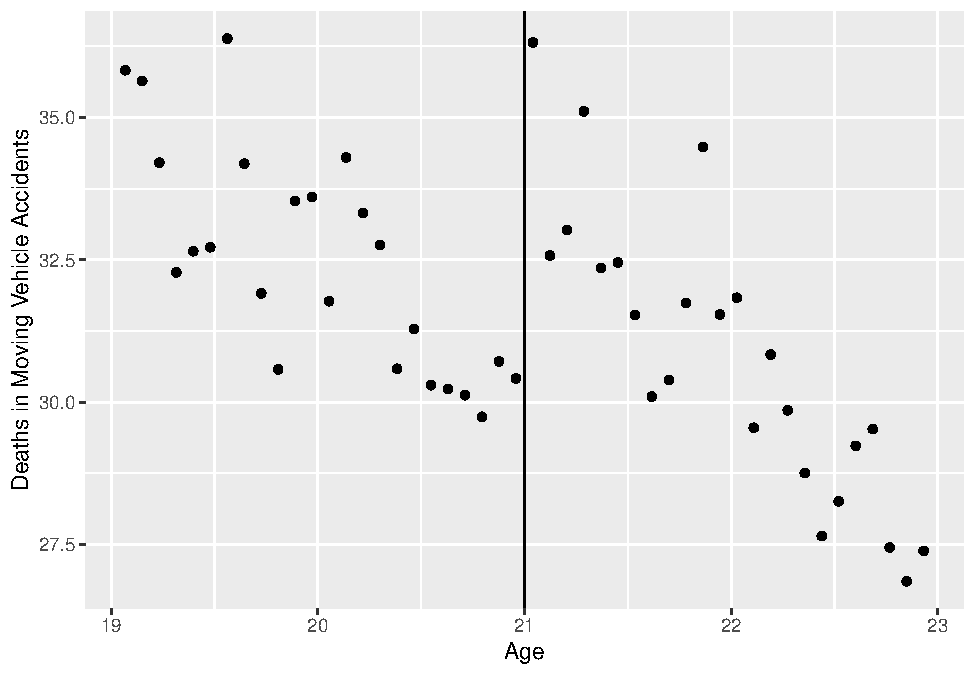
\includegraphics{bailey_files/figure-latex/unnamed-chunk-116-1.pdf}

There appears to be a discontinuity at age 21. Let's estimate the RD model \[mva = \beta_0+\beta_1T+\beta_2(agecell-21)+\epsilon\]\\
where\\
\[\begin{aligned}
T &= 1 \text{ if agecell} \geq 21 \\
T &= 0 \text{ if agecell} < 21
\end{aligned}\]

We will make use of the \texttt{tidyverse} verb \texttt{mutate} and pipe operators from the \texttt{magrittr} package to create \emph{D}\footnote{Recall we will use \emph{D} to avoid the ambiguity of \emph{T} as a variable name.}.

\begin{Shaded}
\begin{Highlighting}[]
\NormalTok{mlda }\OperatorTok\StringTok{ }
\StringTok{  }\KeywordTok{mutate}\NormalTok{(}\DataTypeTok{D =} \KeywordTok{ifelse}\NormalTok{(agecell }\OperatorTok{>=}\StringTok{ }\DecValTok{21}\NormalTok{, }\DecValTok{1}\NormalTok{, }\DecValTok{0}\NormalTok{)) }\OperatorTok\StringTok{ }
\StringTok{  }\KeywordTok{lm}\NormalTok{(mva }\OperatorTok{~}\StringTok{ }\NormalTok{D }\OperatorTok{+}\StringTok{ }\KeywordTok{I}\NormalTok{(agecell }\OperatorTok{-}\StringTok{ }\DecValTok{21}\NormalTok{)) }\OperatorTok\StringTok{ }
\StringTok{  }\KeywordTok{summary}\NormalTok{()}
\end{Highlighting}
\end{Shaded}

\begin{verbatim}

Call:
lm(formula = mva ~ D + I(agecell - 21))

Residuals:
   Min     1Q Median     3Q    Max 
-2.532 -0.849 -0.180  0.758  3.309 

Coefficients:
                Estimate Std. Error t value             Pr(>|t|)    
(Intercept)       29.356      0.429   68.39 < 0.0000000000000002 ***
D                  4.534      0.768    5.90      0.0000004338310 ***
I(agecell - 21)   -3.149      0.337   -9.34      0.0000000000043 ***
---
Signif. codes:  0 '***' 0.001 '**' 0.01 '*' 0.05 '.' 0.1 ' ' 1

Residual standard error: 1.33 on 45 degrees of freedom
  (2 observations deleted due to missingness)
Multiple R-squared:  0.703, Adjusted R-squared:  0.689 
F-statistic: 53.1 on 2 and 45 DF,  p-value: 0.00000000000142
\end{verbatim}

\hypertarget{varying-slopes}{%
\section{Varying Slopes}\label{varying-slopes}}

Let's estimate the relationship described above with a varying slopes RD model. The model now has the form: \[mva = \beta_0+\beta_1T+\beta_2(agecell-21)+\beta_3(agecell-21)T+\epsilon\]\\
where\\
\[T = 1 \text{ if agecell}\geq21\] \[T = 0 \text{ if agecell}<21\]

\begin{Shaded}
\begin{Highlighting}[]
\NormalTok{mlda }\OperatorTok\StringTok{ }
\StringTok{  }\KeywordTok{mutate}\NormalTok{(}\DataTypeTok{D =} \KeywordTok{ifelse}\NormalTok{(agecell }\OperatorTok{>=}\StringTok{ }\DecValTok{21}\NormalTok{, }\DecValTok{1}\NormalTok{, }\DecValTok{0}\NormalTok{)) }\OperatorTok\StringTok{ }
\StringTok{  }\KeywordTok{lm}\NormalTok{(mva }\OperatorTok{~}\StringTok{ }\NormalTok{D }\OperatorTok{*}\StringTok{ }\KeywordTok{I}\NormalTok{(agecell }\OperatorTok{-}\StringTok{ }\DecValTok{21}\NormalTok{)) }\OperatorTok\StringTok{ }
\StringTok{  }\KeywordTok{summary}\NormalTok{()}
\end{Highlighting}
\end{Shaded}

\begin{verbatim}

Call:
lm(formula = mva ~ D * I(agecell - 21))

Residuals:
   Min     1Q Median     3Q    Max 
-2.412 -0.777 -0.291  0.850  3.238 

Coefficients:
                  Estimate Std. Error t value             Pr(>|t|)    
(Intercept)         29.929      0.531   56.39 < 0.0000000000000002 ***
D                    4.534      0.751    6.04           0.00000029 ***
I(agecell - 21)     -2.568      0.466   -5.51           0.00000177 ***
D:I(agecell - 21)   -1.162      0.659   -1.76                0.085 .  
---
Signif. codes:  0 '***' 0.001 '**' 0.01 '*' 0.05 '.' 0.1 ' ' 1

Residual standard error: 1.3 on 44 degrees of freedom
  (2 observations deleted due to missingness)
Multiple R-squared:  0.722, Adjusted R-squared:  0.703 
F-statistic: 38.1 on 3 and 44 DF,  p-value: 0.00000000000267
\end{verbatim}

\hypertarget{plot-rd-model}{%
\section{Plot RD Model}\label{plot-rd-model}}

Use \texttt{ggplot} to plot the RD model. We include plots with an simple regression and an RD model.

\begin{Shaded}
\begin{Highlighting}[]
\NormalTok{mlda }\OperatorTok\StringTok{ }
\StringTok{  }\KeywordTok{select}\NormalTok{(agecell, mva) }\OperatorTok\StringTok{ }
\StringTok{  }\KeywordTok{mutate}\NormalTok{(}\DataTypeTok{D =} \KeywordTok{as.factor}\NormalTok{(}\KeywordTok{ifelse}\NormalTok{(agecell }\OperatorTok{>=}\StringTok{ }\DecValTok{21}\NormalTok{, }\DecValTok{1}\NormalTok{, }\DecValTok{0}\NormalTok{))) }\OperatorTok\StringTok{ }
\StringTok{  }\KeywordTok{ggplot}\NormalTok{(}\KeywordTok{aes}\NormalTok{(}\DataTypeTok{x =}\NormalTok{ agecell, }\DataTypeTok{y =}\NormalTok{ mva)) }\OperatorTok{+}
\StringTok{  }\KeywordTok{geom_point}\NormalTok{(}\KeywordTok{aes}\NormalTok{(}\DataTypeTok{color =}\NormalTok{ D)) }\OperatorTok{+}\StringTok{ }
\StringTok{  }\KeywordTok{geom_smooth}\NormalTok{(}\DataTypeTok{method =} \StringTok{"lm"}\NormalTok{)}
\end{Highlighting}
\end{Shaded}

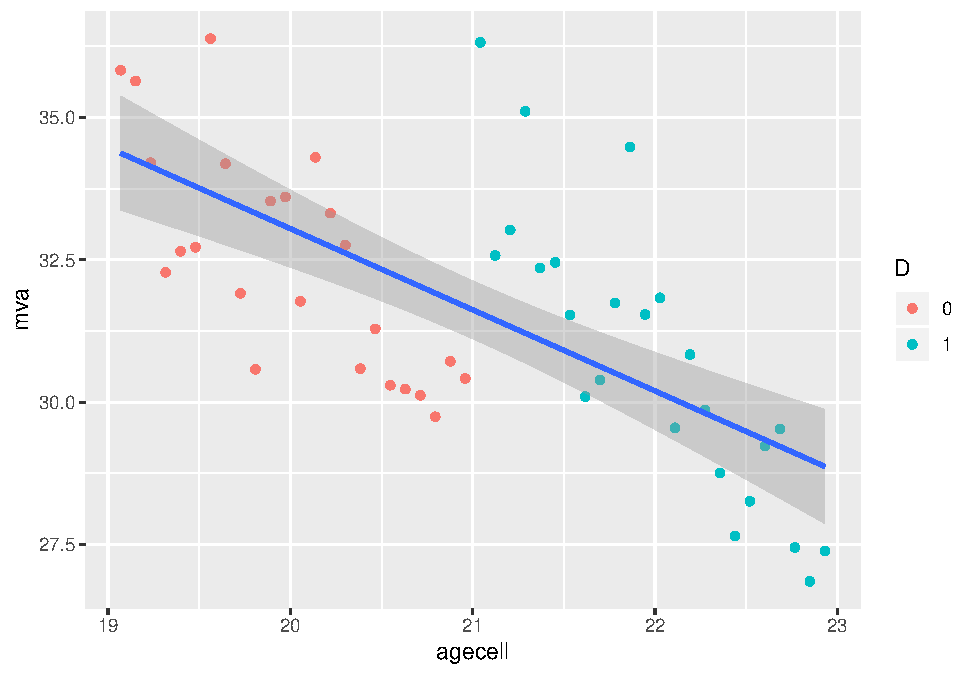
\includegraphics{bailey_files/figure-latex/unnamed-chunk-119-1.pdf}

\begin{Shaded}
\begin{Highlighting}[]
\NormalTok{mlda }\OperatorTok\StringTok{ }
\StringTok{  }\KeywordTok{select}\NormalTok{(agecell, mva) }\OperatorTok\StringTok{ }
\StringTok{  }\KeywordTok{mutate}\NormalTok{(}\DataTypeTok{D =} \KeywordTok{as.factor}\NormalTok{(}\KeywordTok{ifelse}\NormalTok{(agecell }\OperatorTok{>=}\StringTok{ }\DecValTok{21}\NormalTok{, }\DecValTok{1}\NormalTok{, }\DecValTok{0}\NormalTok{))) }\OperatorTok\StringTok{ }
\StringTok{  }\KeywordTok{ggplot}\NormalTok{(}\KeywordTok{aes}\NormalTok{(}\DataTypeTok{x =}\NormalTok{ agecell, }\DataTypeTok{y =}\NormalTok{ mva, }\DataTypeTok{color =}\NormalTok{ D)) }\OperatorTok{+}
\StringTok{  }\KeywordTok{geom_point}\NormalTok{() }\OperatorTok{+}\StringTok{ }
\StringTok{  }\KeywordTok{geom_smooth}\NormalTok{(}\DataTypeTok{method =} \StringTok{"lm"}\NormalTok{)}
\end{Highlighting}
\end{Shaded}

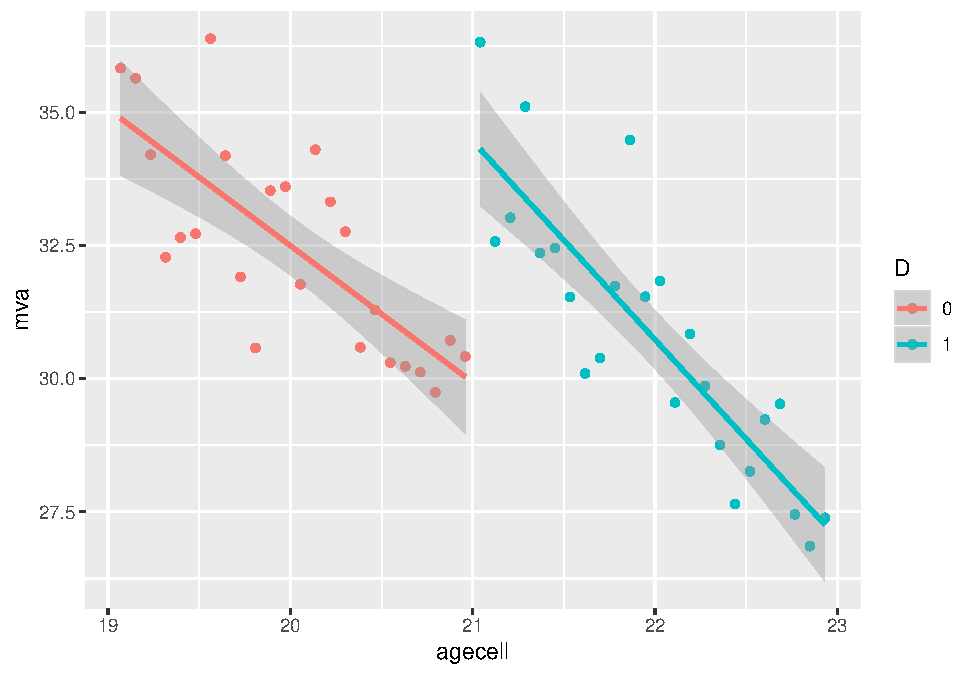
\includegraphics{bailey_files/figure-latex/unnamed-chunk-119-2.pdf}

\hypertarget{rddtools-package}{%
\section{\texorpdfstring{\texttt{rddtools} package}{rddtools package}}\label{rddtools-package}}

We can estimate RD models with the \texttt{rddtools} package\footnote{\texttt{?rddtools} for more.}. To estimate an RD model with \texttt{rddtools} first create an \texttt{rdd\_data} object as follows: \texttt{rdd\_data(y\ =\ df\$y,\ x\ =\ df\$x,\ cutpoint\ =\ C)}. Use the \texttt{rdd\_data} object with \texttt{rdd\_reg\_lm} to estimate the model.

\hypertarget{same-slope-1}{%
\subsection{Same slope}\label{same-slope-1}}

To estimate an RD model with a constant slope call the argument \texttt{rdd\_reg\_lm(rdd\_object,\ slope\ =\ "same")}

\begin{Shaded}
\begin{Highlighting}[]
\KeywordTok{library}\NormalTok{(rddtools)}
\KeywordTok{rdd_data}\NormalTok{(mlda}\OperatorTok{$}\NormalTok{mva, mlda}\OperatorTok{$}\NormalTok{agecell, }\DataTypeTok{cutpoint =} \DecValTok{21}\NormalTok{) }\OperatorTok\StringTok{ }
\StringTok{  }\KeywordTok{rdd_reg_lm}\NormalTok{(}\DataTypeTok{slope =} \StringTok{"same"}\NormalTok{) }\OperatorTok\StringTok{ }
\StringTok{  }\KeywordTok{summary}\NormalTok{()}
\end{Highlighting}
\end{Shaded}

\begin{verbatim}

Call:
lm(formula = y ~ ., data = dat_step1, weights = weights)

Residuals:
   Min     1Q Median     3Q    Max 
-2.532 -0.849 -0.180  0.758  3.309 

Coefficients:
            Estimate Std. Error t value             Pr(>|t|)    
(Intercept)   29.356      0.429   68.39 < 0.0000000000000002 ***
D              4.534      0.768    5.90      0.0000004338310 ***
x             -3.149      0.337   -9.34      0.0000000000043 ***
---
Signif. codes:  0 '***' 0.001 '**' 0.01 '*' 0.05 '.' 0.1 ' ' 1

Residual standard error: 1.33 on 45 degrees of freedom
  (2 observations deleted due to missingness)
Multiple R-squared:  0.703, Adjusted R-squared:  0.689 
F-statistic: 53.1 on 2 and 45 DF,  p-value: 0.00000000000142
\end{verbatim}

Note the results are the same as above.

\hypertarget{varying-slopes-1}{%
\subsection{Varying Slopes}\label{varying-slopes-1}}

To estimate an RD model with varying slopes, change the slope argument to ``separate''.

\begin{Shaded}
\begin{Highlighting}[]
\KeywordTok{rdd_data}\NormalTok{(mlda}\OperatorTok{$}\NormalTok{mva, mlda}\OperatorTok{$}\NormalTok{agecell, }\DataTypeTok{cutpoint =} \DecValTok{21}\NormalTok{) }\OperatorTok\StringTok{ }
\StringTok{  }\KeywordTok{rdd_reg_lm}\NormalTok{(}\DataTypeTok{slope =} \StringTok{"separate"}\NormalTok{) }\OperatorTok\StringTok{ }
\StringTok{  }\KeywordTok{summary}\NormalTok{()}
\end{Highlighting}
\end{Shaded}

\begin{verbatim}

Call:
lm(formula = y ~ ., data = dat_step1, weights = weights)

Residuals:
   Min     1Q Median     3Q    Max 
-2.412 -0.777 -0.291  0.850  3.238 

Coefficients:
            Estimate Std. Error t value             Pr(>|t|)    
(Intercept)   29.929      0.531   56.39 < 0.0000000000000002 ***
D              4.534      0.751    6.04           0.00000029 ***
x             -2.568      0.466   -5.51           0.00000177 ***
x_right       -1.162      0.659   -1.76                0.085 .  
---
Signif. codes:  0 '***' 0.001 '**' 0.01 '*' 0.05 '.' 0.1 ' ' 1

Residual standard error: 1.3 on 44 degrees of freedom
  (2 observations deleted due to missingness)
Multiple R-squared:  0.722, Adjusted R-squared:  0.703 
F-statistic: 38.1 on 3 and 44 DF,  p-value: 0.00000000000267
\end{verbatim}

\hypertarget{scatter-plot}{%
\subsection{Scatter Plot}\label{scatter-plot}}

\begin{Shaded}
\begin{Highlighting}[]
\KeywordTok{rdd_data}\NormalTok{(mlda}\OperatorTok{$}\NormalTok{mva, mlda}\OperatorTok{$}\NormalTok{agecell, }\DataTypeTok{cutpoint =} \DecValTok{21}\NormalTok{) }\OperatorTok\StringTok{ }
\StringTok{  }\KeywordTok{rdd_reg_lm}\NormalTok{(}\DataTypeTok{slope =} \StringTok{"same"}\NormalTok{) }\OperatorTok\StringTok{ }
\StringTok{  }\KeywordTok{plot}\NormalTok{()}
\end{Highlighting}
\end{Shaded}

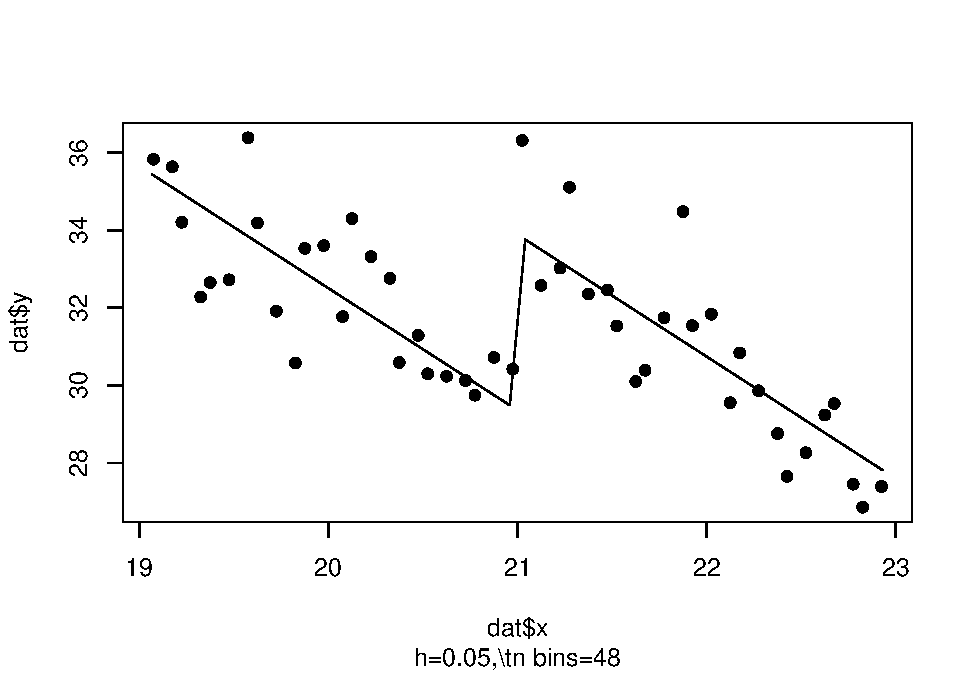
\includegraphics{bailey_files/figure-latex/unnamed-chunk-122-1.pdf}

\begin{Shaded}
\begin{Highlighting}[]
\KeywordTok{rdd_data}\NormalTok{(mlda}\OperatorTok{$}\NormalTok{mva, mlda}\OperatorTok{$}\NormalTok{agecell, }\DataTypeTok{cutpoint =} \DecValTok{21}\NormalTok{) }\OperatorTok\StringTok{ }
\StringTok{  }\KeywordTok{rdd_reg_lm}\NormalTok{(}\DataTypeTok{slope =} \StringTok{"separate"}\NormalTok{) }\OperatorTok\StringTok{ }
\StringTok{  }\KeywordTok{plot}\NormalTok{()}
\end{Highlighting}
\end{Shaded}

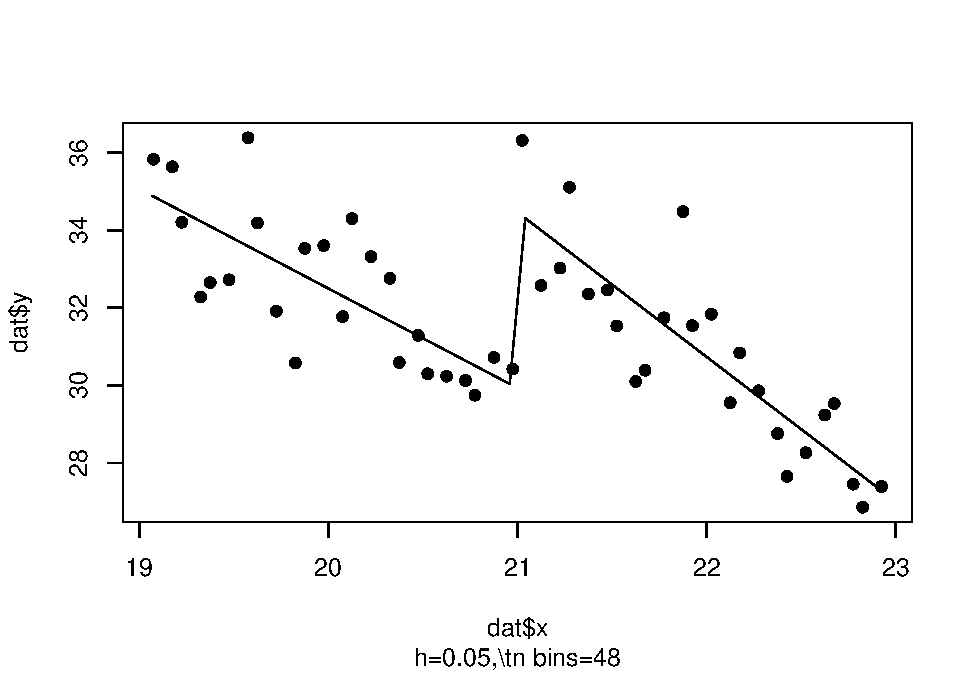
\includegraphics{bailey_files/figure-latex/unnamed-chunk-122-2.pdf}

\hypertarget{chp12}{%
\chapter{Dummy Dependent Variables}\label{chp12}}

We will learn techniques in R to estimate and interpret models in which the dependent variable is categorical. In particular we will learn to estimate linear probability models, probit models, and logit models. We will use the libraries below.

\begin{Shaded}
\begin{Highlighting}[]
\KeywordTok{data}\NormalTok{(mtcars)}
\KeywordTok{library}\NormalTok{(tidyverse)}
\KeywordTok{library}\NormalTok{(magrittr)}
\KeywordTok{library}\NormalTok{(broom)}
\end{Highlighting}
\end{Shaded}

\hypertarget{probit-estimation}{%
\section{Probit Estimation}\label{probit-estimation}}

The probit model is given by \[Pr(Y_i=1)=\Phi(\beta_0+\beta_1X_{1i})\] where \(\Phi()\) is the standard normal CDF. Let's make use of the \texttt{mtcars}\footnote{\texttt{?mtcars} for a reminder.} data set to estimate a probit model to determine engine type as a function of mpg. Engine type, \emph{vs}, is coded as 0 for V-shaped and 1 for straight.

\hypertarget{eda}{%
\subsection{EDA}\label{eda}}

Let's look at a scatter plot and a box plot of \emph{mpg} vs \emph{vs}.

\begin{Shaded}
\begin{Highlighting}[]
\NormalTok{mtcars }\OperatorTok\StringTok{ }
\StringTok{  }\KeywordTok{ggplot}\NormalTok{(}\KeywordTok{aes}\NormalTok{(}\DataTypeTok{x =}\NormalTok{ mpg, }\DataTypeTok{y =}\NormalTok{ vs)) }\OperatorTok{+}\StringTok{ }
\StringTok{  }\KeywordTok{geom_point}\NormalTok{()}
\end{Highlighting}
\end{Shaded}

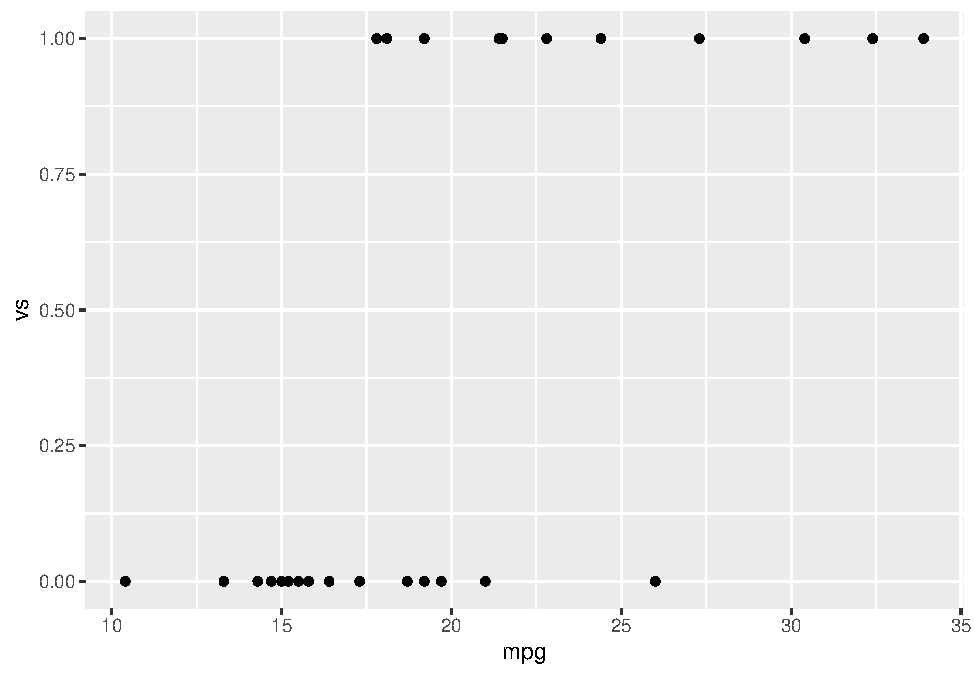
\includegraphics{bailey_files/figure-latex/unnamed-chunk-125-1.pdf}

\begin{Shaded}
\begin{Highlighting}[]
\NormalTok{mtcars }\OperatorTok\StringTok{ }
\StringTok{  }\KeywordTok{mutate}\NormalTok{(}\DataTypeTok{vs =} \KeywordTok{as.factor}\NormalTok{(vs)) }\OperatorTok\StringTok{ }
\StringTok{  }\KeywordTok{ggplot}\NormalTok{(}\KeywordTok{aes}\NormalTok{(}\DataTypeTok{x =}\NormalTok{ vs, }\DataTypeTok{y =}\NormalTok{ mpg)) }\OperatorTok{+}\StringTok{ }
\StringTok{  }\KeywordTok{geom_boxplot}\NormalTok{()}
\end{Highlighting}
\end{Shaded}

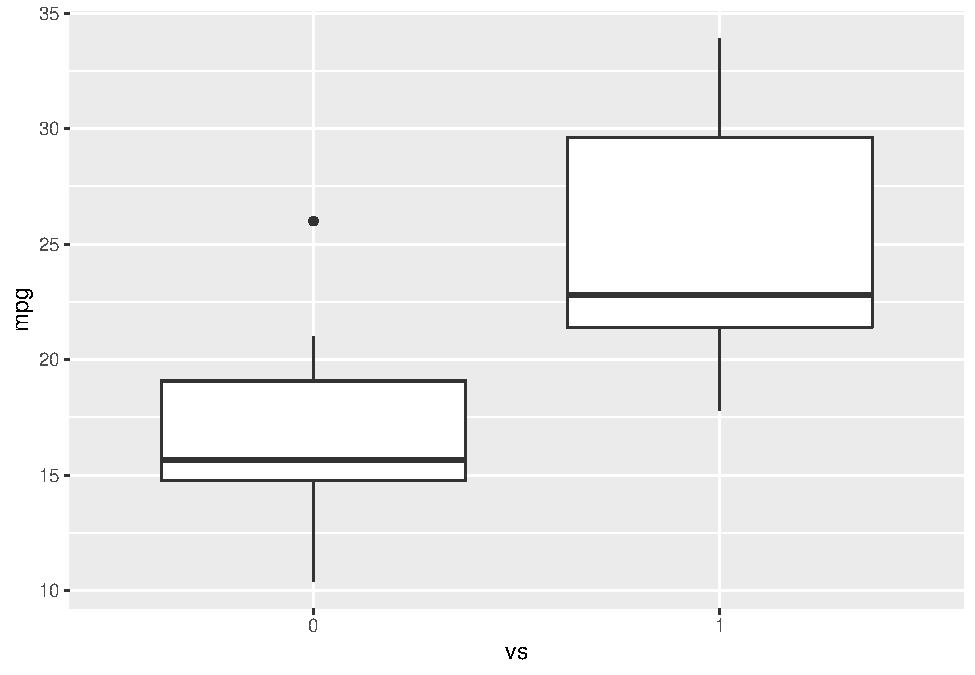
\includegraphics{bailey_files/figure-latex/unnamed-chunk-125-2.pdf}

The boxplot indicates that there is difference in mpg between straight vs v-shaped engines. Note the difference in the code between the two similar calls. We need to treat \emph{vs} as a factor in the boxplot but not in the scatter diagram.

\hypertarget{estimate-the-model}{%
\subsection{Estimate the model}\label{estimate-the-model}}

Let's estimate the probit model \(Pr(vs_i=1)=\Phi(\beta_0+\beta_1mpg_i)\). \texttt{glm} is used to fit dummy dependent variable models.\footnote{These models are also known as limited dependent variable models or limdep models.} To estimate the probit model \texttt{glm} requires three arguments: \texttt{formula}, \texttt{family}, and \texttt{data}. You are familiar with the data and formula arguments. The family argument is description of the error distribution. In this case our family argument will be \texttt{binomial(link\ =\ "probit")}.

\begin{Shaded}
\begin{Highlighting}[]
\NormalTok{mtcars }\OperatorTok\StringTok{ }
\StringTok{  }\KeywordTok{glm}\NormalTok{(vs }\OperatorTok{~}\StringTok{ }\NormalTok{mpg, }\DataTypeTok{family =} \KeywordTok{binomial}\NormalTok{(}\DataTypeTok{link =} \StringTok{"probit"}\NormalTok{)) }\OperatorTok\StringTok{ }
\StringTok{  }\KeywordTok{tidy}\NormalTok{()}
\end{Highlighting}
\end{Shaded}

\begin{verbatim}
# A tibble: 2 x 5
  term        estimate std.error statistic p.value
  <chr>          <dbl>     <dbl>     <dbl>   <dbl>
1 (Intercept)   -5.09     1.64       -3.10 0.00193
2 mpg            0.246    0.0825      2.98 0.00286
\end{verbatim}

\hypertarget{estimated-effects}{%
\subsection{Estimated Effects}\label{estimated-effects}}

\hypertarget{discrete-difference}{%
\subsubsection{Discrete Difference}\label{discrete-difference}}

\hypertarget{x_1-is-continuous}{%
\paragraph{\texorpdfstring{\(X_1\) is Continuous}{X\_1 is Continuous}}\label{x_1-is-continuous}}

To estimate the effect of a change in the independent variable on the probability of observing the dependent variable we need to calculate the average difference between the fitted values of the model, \emph{P1}, and the predicted values of the model when the independent variable we are interested in is changed by one standard deviation, \emph{P2}.

Fitted values, \emph{P1}, are easily obtained from the glm object as follows:

\begin{Shaded}
\begin{Highlighting}[]
\NormalTok{vs_glm <-}
\StringTok{  }\NormalTok{mtcars }\OperatorTok
\StringTok{  }\KeywordTok{glm}\NormalTok{(vs }\OperatorTok{~}\StringTok{ }\NormalTok{mpg, }\DataTypeTok{family =} \KeywordTok{binomial}\NormalTok{(}\DataTypeTok{link =} \StringTok{"probit"}\NormalTok{))}
\NormalTok{P1 <-}\StringTok{ }\NormalTok{vs_glm}\OperatorTok{$}\NormalTok{fitted}
\end{Highlighting}
\end{Shaded}

The fitted variables have had \texttt{pnorm()} applied to the linear estimates, so they are \emph{P1}.

To obtain marginal effects, we need to let \emph{mpg} vary by one standard deviation and obtain the predicted values from the estimated equation. To find \emph{P2}, the predicted values resulting from a one standard deviation change in the independent variable, we will make use of \texttt{predict.glm}. \texttt{predict.glm}\footnote{\texttt{?predict.glm} for more information.} will require two arguments to estimate \emph{P2}, the equation object and the newdata \texttt{predict.glm(object,\ newdata\ =\ df}. Unfortunately the expose pipe \texttt{\%\$\%} does not function with \texttt{predict.glm}, so we will have to create a data frame of the changed independent variable. We will use the \texttt{dplyr} verbs \texttt{select} and \texttt{mutate} to create the new data frame. We calculate \emph{P2} below:

\begin{Shaded}
\begin{Highlighting}[]
\CommentTok{# Create the new data}
\NormalTok{newdata <-}\StringTok{ }
\NormalTok{mtcars }\OperatorTok\StringTok{ }
\StringTok{  }\NormalTok{dplyr}\OperatorTok{::}\KeywordTok{select}\NormalTok{(mpg) }\OperatorTok\StringTok{ }\CommentTok{#I used this form to avoid the conflict with select in the MASS package}
\StringTok{  }\KeywordTok{mutate}\NormalTok{(}\DataTypeTok{mpg =}\NormalTok{ mpg }\OperatorTok{+}\StringTok{ }\KeywordTok{sd}\NormalTok{(mpg))}
\CommentTok{# Create P2}
\NormalTok{P2 <-}\StringTok{ }
\StringTok{  }\KeywordTok{predict.glm}\NormalTok{(vs_glm, newdata) }\OperatorTok\StringTok{ }
\StringTok{  }\KeywordTok{pnorm}\NormalTok{()}
\CommentTok{# Marginal Effect}
\KeywordTok{mean}\NormalTok{(P2}\OperatorTok{-}\NormalTok{P1)}
\end{Highlighting}
\end{Shaded}

\begin{verbatim}
[1] 0.339
\end{verbatim}

So, a one standard deviation increase in \emph{mpg} will yield a 33.89\% increase in the probability that the car has straight engine.

\hypertarget{independent-variable-is-a-dummy.}{%
\paragraph{Independent variable is a dummy.}\label{independent-variable-is-a-dummy.}}

Let's add \emph{am}, transmission type, to the model. \emph{am} is coded as 0 if the car has an automatic transmission and 1 if it has a manual transmission. First, estimate the model \(Pr(vs_i=1)=\Phi(\beta_0+\beta_1am+\beta_2mpg_i)\).

\begin{Shaded}
\begin{Highlighting}[]
\NormalTok{mtcars }\OperatorTok
\StringTok{  }\KeywordTok{glm}\NormalTok{(vs }\OperatorTok{~}\StringTok{ }\NormalTok{am }\OperatorTok{+}\StringTok{ }\NormalTok{mpg, }\DataTypeTok{family =} \KeywordTok{binomial}\NormalTok{(}\DataTypeTok{link =} \StringTok{"probit"}\NormalTok{))}
\end{Highlighting}
\end{Shaded}

\begin{verbatim}

Call:  glm(formula = vs ~ am + mpg, family = binomial(link = "probit"))

Coefficients:
(Intercept)           am          mpg  
      -7.47        -1.84         0.40  

Degrees of Freedom: 31 Total (i.e. Null);  29 Residual
Null Deviance:      43.9 
Residual Deviance: 20.3     AIC: 26.3
\end{verbatim}

We will follow similar steps as those above to interpret a change from automatic to manual transmission on the probability that the engine is straight. We will estimate \emph{P0}, the fitted values, when \emph{am} = 0, and \emph{P1}, the fitted values when \emph{am} = 1.

\begin{Shaded}
\begin{Highlighting}[]
\CommentTok{# Estimate the model}
\NormalTok{vs_am_glm <-}\StringTok{ }
\StringTok{  }\NormalTok{mtcars }\OperatorTok
\StringTok{  }\KeywordTok{glm}\NormalTok{(vs }\OperatorTok{~}\StringTok{ }\NormalTok{am }\OperatorTok{+}\StringTok{ }\NormalTok{mpg, }\DataTypeTok{family =} \KeywordTok{binomial}\NormalTok{(}\DataTypeTok{link =} \StringTok{"probit"}\NormalTok{))}
\CommentTok{# P0}
\NormalTok{newdata <-}\StringTok{ }
\StringTok{  }\NormalTok{mtcars }\OperatorTok\StringTok{ }
\StringTok{  }\NormalTok{dplyr}\OperatorTok{::}\KeywordTok{select}\NormalTok{(am, mpg) }\OperatorTok\StringTok{ }
\StringTok{  }\KeywordTok{mutate}\NormalTok{(}\DataTypeTok{am =} \DecValTok{0}\NormalTok{)}
\NormalTok{P0 <-}\StringTok{ }
\StringTok{  }\KeywordTok{predict.glm}\NormalTok{(vs_am_glm, newdata) }\OperatorTok\StringTok{ }
\StringTok{  }\KeywordTok{pnorm}\NormalTok{()}
\CommentTok{# P1}
\NormalTok{newdata <-}\StringTok{ }
\StringTok{  }\NormalTok{mtcars }\OperatorTok\StringTok{ }
\StringTok{  }\NormalTok{dplyr}\OperatorTok{::}\KeywordTok{select}\NormalTok{(am, mpg) }\OperatorTok\StringTok{ }
\StringTok{  }\KeywordTok{mutate}\NormalTok{(}\DataTypeTok{am =} \DecValTok{1}\NormalTok{)}
\NormalTok{P1 <-}\StringTok{ }
\StringTok{  }\KeywordTok{predict.glm}\NormalTok{(vs_am_glm, newdata) }\OperatorTok\StringTok{ }
\StringTok{  }\KeywordTok{pnorm}\NormalTok{()}
\KeywordTok{mean}\NormalTok{(P1}\OperatorTok{-}\NormalTok{P0)}
\end{Highlighting}
\end{Shaded}

\begin{verbatim}
[1] -0.269
\end{verbatim}

A car with an manual transmission is 26.9\% less likely, on average, to have a straight engine, \emph{ceteris paribus}.

\hypertarget{marginal-effects}{%
\subsubsection{Marginal Effects}\label{marginal-effects}}

If \(X_1\) is continuous we can estimate the marginal effects of a change in \(X_1\) as \(\phi(\hat\beta_0+\hat\beta_1X_{1i}+\hat\beta_2X_{2i})\hat\beta_1\). Where \(\phi()\) is the normal PDF. Let's estimate the marginal effect of \emph{mpg} on \emph{vs} using the model above.

\begin{Shaded}
\begin{Highlighting}[]
\NormalTok{marg_effect <-}\StringTok{ }
\KeywordTok{dnorm}\NormalTok{(vs_am_glm}\OperatorTok{$}\NormalTok{coef[}\DecValTok{1}\NormalTok{] }\OperatorTok{+}\StringTok{ }\NormalTok{vs_am_glm}\OperatorTok{$}\NormalTok{coef[}\DecValTok{2}\NormalTok{]}\OperatorTok{*}\NormalTok{mtcars}\OperatorTok{$}\NormalTok{am }\OperatorTok{+}\StringTok{ }\NormalTok{vs_am_glm}\OperatorTok{$}\NormalTok{coef[}\DecValTok{3}\NormalTok{]}\OperatorTok{*}\NormalTok{mtcars}\OperatorTok{$}\NormalTok{mpg) }\OperatorTok{*}\StringTok{ }\NormalTok{vs_am_glm}\OperatorTok{$}\NormalTok{coef[}\DecValTok{3}\NormalTok{]}
\KeywordTok{mean}\NormalTok{(marg_effect)}
\end{Highlighting}
\end{Shaded}

\begin{verbatim}
[1] 0.0692
\end{verbatim}

The marginal effect of \emph{mpg} on type of engine is 0.069.

\hypertarget{mfx-and-margins-packages}{%
\paragraph{\texorpdfstring{\texttt{mfx} and \texttt{margins} Packages}{mfx and margins Packages}}\label{mfx-and-margins-packages}}

We can use the \texttt{mfx} and \texttt{margins} packages to estimate the marginal effect of a continuous variable directly from the model we estimate. \texttt{mfx::probitmfx(formula,\ data,\ atmean\ =\ F)} and \texttt{margins::margins(model)} are the respective function calls to estimate marginal effects from the two packages.

\begin{Shaded}
\begin{Highlighting}[]
\CommentTok{# mfx}
\NormalTok{mfx}\OperatorTok{::}\KeywordTok{probitmfx}\NormalTok{(vs_am_glm, mtcars, }\DataTypeTok{atmean =}\NormalTok{ F)}
\end{Highlighting}
\end{Shaded}

\begin{verbatim}
Call:
mfx::probitmfx(formula = vs_am_glm, data = mtcars, atmean = F)

Marginal Effects:
       dF/dx Std. Err.     z               P>|z|    
am  -0.26942   0.09154 -2.94              0.0032 ** 
mpg  0.06925   0.00765  9.05 <0.0000000000000002 ***
---
Signif. codes:  0 '***' 0.001 '**' 0.01 '*' 0.05 '.' 0.1 ' ' 1

dF/dx is for discrete change for the following variables:

[1] "am"
\end{verbatim}

Note that these values are identically to the ones calculated by hand above.

\begin{Shaded}
\begin{Highlighting}[]
\CommentTok{# margins}
\NormalTok{margins}\OperatorTok{::}\KeywordTok{margins}\NormalTok{(vs_am_glm, }\DataTypeTok{data =}\NormalTok{ mtcars)}
\end{Highlighting}
\end{Shaded}

\begin{verbatim}
      am     mpg
 -0.3185 0.06925
\end{verbatim}

The marginal effect of \emph{mpg} is the same, while the effect of \emph{am} is similar. \texttt{?margins} or \href{https://cran.r-project.org/web/packages/margins/vignettes/Introduction.html\#references}{An Introduction to `margins'} for more on the \texttt{margins} package.

\hypertarget{logit-estimation}{%
\section{Logit Estimation}\label{logit-estimation}}

The logit model takes the form \(Pr(Y_i=1)=\frac{e^{\beta_0+\beta_1X_{1i}}}{1+e^{\beta_0+\beta_1X_{1i}}}\) An alternative form of the logit model might be easier to interpret. With appropriate algebraic gymnastics we can write the logistic model as \(\ln(\frac{p_i}{1-p_i})=\beta_0+\beta_1X_{1i}\), where \(\ln(\frac{p_1}{1-p_i})\) is the log of the odds ratio.

Let's estimate the model from above as a logit rather than a probit. All we need to do is change the link argument to logit to estimate the model.

\begin{Shaded}
\begin{Highlighting}[]
\NormalTok{mtcars }\OperatorTok
\StringTok{  }\KeywordTok{glm}\NormalTok{(vs }\OperatorTok{~}\StringTok{ }\NormalTok{mpg }\OperatorTok{+}\StringTok{ }\NormalTok{am, }\DataTypeTok{family =} \KeywordTok{binomial}\NormalTok{(}\DataTypeTok{link =} \StringTok{"logit"}\NormalTok{))}
\end{Highlighting}
\end{Shaded}

\begin{verbatim}

Call:  glm(formula = vs ~ mpg + am, family = binomial(link = "logit"))

Coefficients:
(Intercept)          mpg           am  
    -12.705        0.681       -3.007  

Degrees of Freedom: 31 Total (i.e. Null);  29 Residual
Null Deviance:      43.9 
Residual Deviance: 20.6     AIC: 26.6
\end{verbatim}

Suppose we'd like to know the probability that a vehicle with automatic transmission that gets 25 mpg has a straight engine. Calculate the odds ratio as \(\ln(\frac{p_1}{1-p_i})=-12.7051+0.6809*25-3.0073*0 = 4.9474\). Exponentiate both sides and solve for \emph{p}. \(e^{\ln(\frac{p_i}{1-p_i})} = e^{4.9474}\). We know that an exponentiated natural log is just itself so we have \(\frac{p_i}{1-p_i}=140.808\). Solving for \emph{p} yields \(p_i=\frac{140.808}{141.808}=.9925\). The probability we are looking for is 99.25\%. So,
\(\hat p=\frac{e^{\hat\beta_0+\hat\beta_1X_1}}{1 + e^{\hat\beta_0+\hat\beta_1X_1}}\).

\hypertarget{discrete-differences}{%
\subsection{Discrete Differences}\label{discrete-differences}}

The discrete-difference can be calculated as the difference in two probabilities. We can estimate the mean change in probability from an increase in \emph{mpg} of 1.

\begin{Shaded}
\begin{Highlighting}[]
\NormalTok{vs_logit <-}\StringTok{ }
\StringTok{  }\NormalTok{mtcars }\OperatorTok
\StringTok{  }\KeywordTok{glm}\NormalTok{(vs }\OperatorTok{~}\StringTok{ }\NormalTok{mpg }\OperatorTok{+}\StringTok{ }\NormalTok{am, }\DataTypeTok{family =} \KeywordTok{binomial}\NormalTok{(}\DataTypeTok{link =} \StringTok{"logit"}\NormalTok{))}
\CommentTok{# p1 are the fitted values of the regression}
\NormalTok{p1 <-}\StringTok{ }\NormalTok{vs_logit}\OperatorTok{$}\NormalTok{fitted}
\CommentTok{# to calculate p2 add one to mpg and find the predicted values}
\NormalTok{newdata <-}\StringTok{ }
\StringTok{  }\NormalTok{mtcars }\OperatorTok\StringTok{ }
\StringTok{  }\NormalTok{dplyr}\OperatorTok{::}\KeywordTok{select}\NormalTok{(mpg, am) }\OperatorTok\StringTok{ }
\StringTok{  }\KeywordTok{mutate}\NormalTok{(}\DataTypeTok{mpg =}\NormalTok{ mpg }\OperatorTok{+}\StringTok{ }\DecValTok{1}\NormalTok{)}
\NormalTok{p2 <-}\StringTok{ }\KeywordTok{exp}\NormalTok{(}\KeywordTok{predict}\NormalTok{(vs_logit, newdata))}\OperatorTok{/}\NormalTok{(}\DecValTok{1}\OperatorTok{+}\KeywordTok{exp}\NormalTok{(}\KeywordTok{predict}\NormalTok{(vs_logit, newdata)))}
\CommentTok{# calcualte the mean difference between the p2 and p1}
\KeywordTok{mean}\NormalTok{(p2}\OperatorTok{-}\NormalTok{p1)}
\end{Highlighting}
\end{Shaded}

\begin{verbatim}
[1] 0.0727
\end{verbatim}

On average an increase of 1 \emph{mpg} will increase the probability the car has straight engine by 7.3\%.

\hypertarget{marginal-effects-1}{%
\subsection{Marginal Effects}\label{marginal-effects-1}}

Use the \texttt{mfx} or \texttt{margins} package to estimate the marginal effects of a change in an independent variable.

\begin{Shaded}
\begin{Highlighting}[]
\CommentTok{# mfx }
\NormalTok{mfx}\OperatorTok{::}\KeywordTok{logitmfx}\NormalTok{(vs_logit, mtcars, }\DataTypeTok{atmean =}\NormalTok{ F)}
\end{Highlighting}
\end{Shaded}

\begin{verbatim}
Call:
mfx::logitmfx(formula = vs_logit, data = mtcars, atmean = F)

Marginal Effects:
      dF/dx Std. Err.     z  P>|z|   
mpg  0.0692    0.0453  1.53 0.1267   
am  -0.2618    0.0941 -2.78 0.0054 **
---
Signif. codes:  0 '***' 0.001 '**' 0.01 '*' 0.05 '.' 0.1 ' ' 1

dF/dx is for discrete change for the following variables:

[1] "am"
\end{verbatim}

\begin{Shaded}
\begin{Highlighting}[]
\CommentTok{# margins}
\NormalTok{margins}\OperatorTok{::}\KeywordTok{margins}\NormalTok{(vs_logit, mtcars)}
\end{Highlighting}
\end{Shaded}

\begin{verbatim}
     mpg      am
 0.06923 -0.3057
\end{verbatim}

\hypertarget{testing-hypotheses}{%
\section{Testing Hypotheses}\label{testing-hypotheses}}

Let's estimate a new probit model \(Pr(vs_i=1)=\Phi(\beta_0+\beta_1am+\beta_2mpg_i+\beta_3hp_i)\) using the \texttt{mtcars} data set and test the hypothesis that our model has overall explanatory power. \[H_0:\beta_1=\beta_2=\beta_3=0\]
vs.~\[\text{@ least one }\beta\ne0\]
We an estimate a restricted model and compare the likelihood ratios to the likelihood ratio of the unrestricted model and perform the LR test where \(LR = 2(\log L_{UR}-\log L_R)\text{~}\chi^2_{df}\). Where the \emph{df} is equal to the number of restrictions or number of equal signs in \(H_0\).

\begin{Shaded}
\begin{Highlighting}[]
\NormalTok{ur_model <-}\StringTok{ }
\StringTok{  }\NormalTok{mtcars }\OperatorTok
\StringTok{  }\KeywordTok{glm}\NormalTok{(vs }\OperatorTok{~}\StringTok{ }\NormalTok{am }\OperatorTok{+}\StringTok{ }\NormalTok{mpg }\OperatorTok{+}\StringTok{ }\NormalTok{hp, }\DataTypeTok{family =} \KeywordTok{binomial}\NormalTok{(}\DataTypeTok{link =} \StringTok{"probit"}\NormalTok{))}
\NormalTok{r_model <-}\StringTok{ }
\StringTok{  }\NormalTok{mtcars }\OperatorTok
\StringTok{  }\KeywordTok{glm}\NormalTok{(vs }\OperatorTok{~}\StringTok{ }\DecValTok{1}\NormalTok{, }\DataTypeTok{family =} \KeywordTok{binomial}\NormalTok{(}\DataTypeTok{link =} \StringTok{"probit"}\NormalTok{))}
\NormalTok{lr <-}\StringTok{ }\DecValTok{2}\OperatorTok{*}\NormalTok{(}\KeywordTok{logLik}\NormalTok{(ur_model)[}\DecValTok{1}\NormalTok{]}\OperatorTok{-}\KeywordTok{logLik}\NormalTok{(r_model)[}\DecValTok{1}\NormalTok{])}
\DecValTok{1} \OperatorTok{-}\StringTok{ }\KeywordTok{pchisq}\NormalTok{(lr, }\DecValTok{3}\NormalTok{)}
\end{Highlighting}
\end{Shaded}

\begin{verbatim}
[1] 0.000000302
\end{verbatim}

We can reject \(H_0\).

Instead, let's use \texttt{lrtest} from the \texttt{lmtest} package to test hypotheses about our limited dependent variable models. We can specify the restrictions as an argument in the call.

\begin{Shaded}
\begin{Highlighting}[]
\NormalTok{lmtest}\OperatorTok{::}\KeywordTok{lrtest}\NormalTok{(ur_model, }\KeywordTok{c}\NormalTok{(}\StringTok{"am"}\NormalTok{, }\StringTok{"mpg"}\NormalTok{, }\StringTok{"hp"}\NormalTok{))}
\end{Highlighting}
\end{Shaded}

\begin{verbatim}
Likelihood ratio test

Model 1: vs ~ am + mpg + hp
Model 2: vs ~ 1
  #Df LogLik Df Chisq Pr(>Chisq)    
1   4  -5.36                        
2   1 -21.93 -3  33.1  0.0000003 ***
---
Signif. codes:  0 '***' 0.001 '**' 0.01 '*' 0.05 '.' 0.1 ' ' 1
\end{verbatim}

Let's test the null hypothesis \[H_0:\beta_2=\beta_3\] \[H_1: \beta_2\ne\beta_3\]
The restricted model becomes \(Pr(vs_i=1)=\Phi(\beta_0+\beta_1am+\beta_2(mpg_i+hp_i))\)

\begin{Shaded}
\begin{Highlighting}[]
\NormalTok{r_model <-}\StringTok{ }
\StringTok{  }\NormalTok{mtcars }\OperatorTok
\StringTok{  }\KeywordTok{glm}\NormalTok{(vs }\OperatorTok{~}\StringTok{ }\NormalTok{am }\OperatorTok{+}\StringTok{ }\KeywordTok{I}\NormalTok{(mpg }\OperatorTok{+}\StringTok{ }\NormalTok{hp), }\DataTypeTok{family =} \KeywordTok{binomial}\NormalTok{(}\DataTypeTok{link =} \StringTok{"probit"}\NormalTok{))}
\NormalTok{lmtest}\OperatorTok{::}\KeywordTok{lrtest}\NormalTok{(ur_model, r_model)}
\end{Highlighting}
\end{Shaded}

\begin{verbatim}
Likelihood ratio test

Model 1: vs ~ am + mpg + hp
Model 2: vs ~ am + I(mpg + hp)
  #Df LogLik Df Chisq Pr(>Chisq)
1   4  -5.36                    
2   3  -6.63 -1  2.53       0.11
\end{verbatim}

We fail to reject \(H_0\) and conclude that we have no evidence to believe that \(\beta_2\ne\beta_3\).

We would test hypotheses concerning logit models in same way.

\hypertarget{graphing-probit-and-logit-models}{%
\section{Graphing Probit and Logit Models}\label{graphing-probit-and-logit-models}}

\begin{Shaded}
\begin{Highlighting}[]
\NormalTok{mtcars }\OperatorTok\StringTok{ }
\StringTok{  }\KeywordTok{ggplot}\NormalTok{(}\KeywordTok{aes}\NormalTok{(}\DataTypeTok{x =}\NormalTok{ mpg, }\DataTypeTok{y =}\NormalTok{ vs)) }\OperatorTok{+}\StringTok{ }
\StringTok{  }\KeywordTok{geom_point}\NormalTok{() }\OperatorTok{+}
\StringTok{  }\KeywordTok{geom_smooth}\NormalTok{(}\DataTypeTok{method =} \StringTok{"glm"}\NormalTok{, }\DataTypeTok{method.args=}\KeywordTok{list}\NormalTok{(}\DataTypeTok{family=}\KeywordTok{binomial}\NormalTok{(}\DataTypeTok{link =} \StringTok{"probit"}\NormalTok{)), }\DataTypeTok{se =}\NormalTok{ F) }\OperatorTok{+}\StringTok{ }
\StringTok{  }\KeywordTok{ggtitle}\NormalTok{(}\StringTok{"Probit"}\NormalTok{)}
\end{Highlighting}
\end{Shaded}

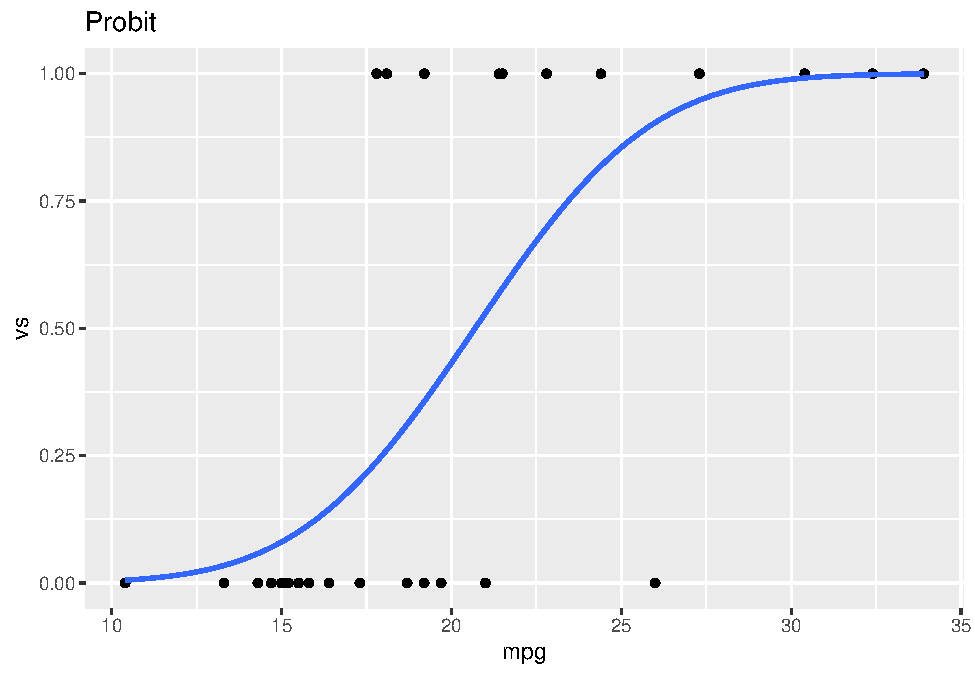
\includegraphics{bailey_files/figure-latex/unnamed-chunk-140-1.pdf}

\begin{Shaded}
\begin{Highlighting}[]
\NormalTok{mtcars }\OperatorTok\StringTok{ }
\StringTok{  }\KeywordTok{ggplot}\NormalTok{(}\KeywordTok{aes}\NormalTok{(}\DataTypeTok{x =}\NormalTok{ mpg, }\DataTypeTok{y =}\NormalTok{ vs)) }\OperatorTok{+}\StringTok{ }
\StringTok{  }\KeywordTok{geom_point}\NormalTok{() }\OperatorTok{+}
\StringTok{  }\KeywordTok{geom_smooth}\NormalTok{(}\DataTypeTok{method =} \StringTok{"glm"}\NormalTok{, }\DataTypeTok{method.args=}\KeywordTok{list}\NormalTok{(}\DataTypeTok{family=}\KeywordTok{binomial}\NormalTok{(}\DataTypeTok{link =} \StringTok{"logit"}\NormalTok{)), }\DataTypeTok{se =}\NormalTok{ F) }\OperatorTok{+}\StringTok{ }
\StringTok{  }\KeywordTok{ggtitle}\NormalTok{(}\StringTok{"Logit"}\NormalTok{)}
\end{Highlighting}
\end{Shaded}

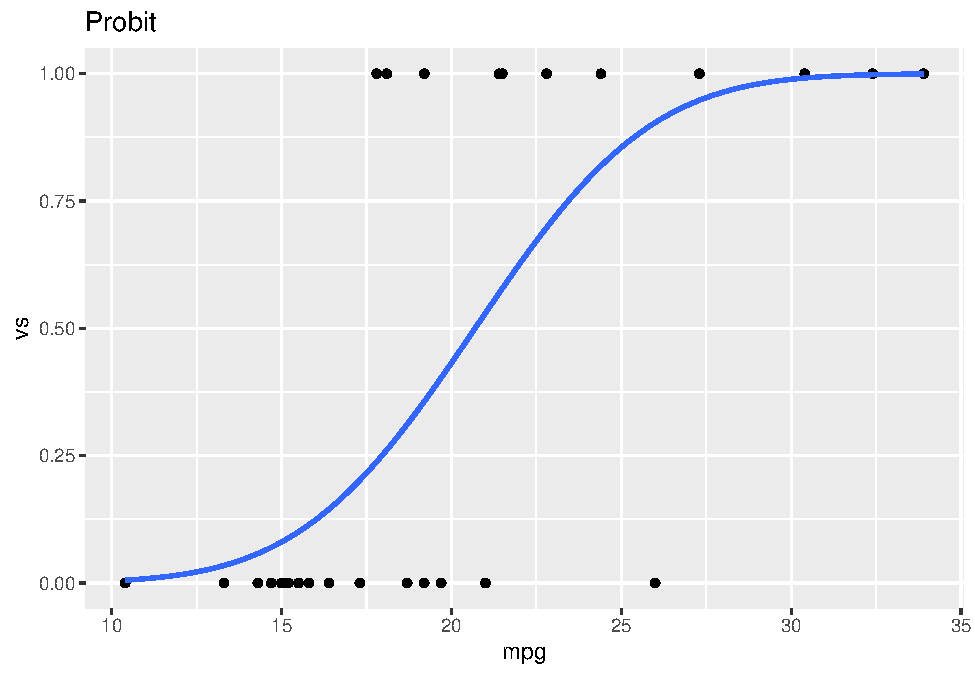
\includegraphics{bailey_files/figure-latex/unnamed-chunk-141-1.pdf}

\hypertarget{chp13}{%
\chapter{Time Series: Dealing with Stickiness over Time}\label{chp13}}

In this chapter we will learn to work with time--series data in R.

\hypertarget{time-series-objects-in-r}{%
\section{Time Series Objects in R}\label{time-series-objects-in-r}}

Working with time-series data in R is simplified if the data are structured as a \emph{time-series object}. There are a host of functions and packages dedicated to time-series data. A time-series object is an R structure that contains the observations, the start and end date of the series, and information about the frequency or periodicity.

We will use the \href{https://archive.ics.uci.edu/ml/machine-learning-databases/00275/}{Bike Sharing Dataset}\footnote{Fanaee-T, Hadi, and Gama, Joao, `Event labeling combining ensemble detectors and background knowledge', Progress in Artificial Intelligence (2013): pp.~1-15, Springer Berlin Heidelberg} from the UCI Machine Learning Repository.

\begin{itemize}
\tightlist
\item
  The data set has 731 observations on 17 variables

  \begin{itemize}
  \tightlist
  \item
    instant: record index
  \item
    dteday : date
  \item
    season : season (1:spring, 2:summer, 3:fall, 4:winter)
  \item
    yr : year (0: 2011, 1:2012)
  \item
    mnth : month ( 1 to 12)
  \item
    hr : hour (0 to 23)
  \item
    holiday : weather day is holiday or not (extracted from \url{http://dchr.dc.gov/page/holiday-schedule})
  \item
    weekday : day of the week
  \item
    workingday : if day is neither weekend nor holiday is 1, otherwise is 0.
  \item
    weathersit :

    \begin{itemize}
    \tightlist
    \item
      1: Clear, Few clouds, Partly cloudy, Partly cloudy
    \item
      2: Mist + Cloudy, Mist + Broken clouds, Mist + Few clouds, Mist
    \item
      3: Light Snow, Light Rain + Thunderstorm + Scattered clouds, Light Rain + Scattered clouds
    \item
      4: Heavy Rain + Ice Pallets + Thunderstorm + Mist, Snow + Fog
    \end{itemize}
  \item
    temp : Normalized temperature in Celsius. The values are divided to 41 (max)
  \item
    atemp: Normalized feeling temperature in Celsius. The values are divided to 50 (max)
  \item
    hum: Normalized humidity. The values are divided to 100 (max)
  \item
    windspeed: Normalized wind speed. The values are divided to 67 (max)
  \item
    casual: count of casual users
  \item
    registered: count of registered users
  \item
    cnt: count of total rental bikes including both casual and registered
  \end{itemize}
\end{itemize}

\begin{Shaded}
\begin{Highlighting}[]
\KeywordTok{library}\NormalTok{(tidyverse)}
\KeywordTok{library}\NormalTok{(broom)}
\KeywordTok{library}\NormalTok{(xts)}
\KeywordTok{library}\NormalTok{(magrittr)}
\NormalTok{bike_share <-}\StringTok{ }\KeywordTok{read_csv}\NormalTok{(}\StringTok{"Data/day.csv"}\NormalTok{)}
\KeywordTok{head}\NormalTok{(bike_share)}
\end{Highlighting}
\end{Shaded}

\begin{verbatim}
# A tibble: 6 x 16
  instant dteday     season    yr  mnth holiday weekday workingday
    <dbl> <date>      <dbl> <dbl> <dbl>   <dbl>   <dbl>      <dbl>
1       1 2011-01-01      1     0     1       0       6          0
2       2 2011-01-02      1     0     1       0       0          0
3       3 2011-01-03      1     0     1       0       1          1
4       4 2011-01-04      1     0     1       0       2          1
5       5 2011-01-05      1     0     1       0       3          1
6       6 2011-01-06      1     0     1       0       4          1
# ... with 8 more variables: weathersit <dbl>, temp <dbl>, atemp <dbl>,
#   hum <dbl>, windspeed <dbl>, casual <dbl>, registered <dbl>, cnt <dbl>
\end{verbatim}

We can convert \texttt{bike\_share} to a time-series object using the \texttt{xts} package. A time-series object requires an index to identify each observation by its date. We create the index with \texttt{seq(as.date("YYYY-MM-DD"),\ by\ =\ "period",\ length.out\ =\ n)}, our start date is 2011-01-01, by ``days'', with the number of observations as the length. After we create the date index, we will use \texttt{dplyr:select} to choose the variables (we don't need \emph{dteday}, \emph{yr}, or \emph{mnth}). As always, we will make use of the pipe operator to complete the code.

\begin{Shaded}
\begin{Highlighting}[]
\NormalTok{dates <-}\StringTok{ }\KeywordTok{seq}\NormalTok{(}\KeywordTok{as.Date}\NormalTok{(}\StringTok{"2011-01-01"}\NormalTok{), }\DataTypeTok{by =} \StringTok{"days"}\NormalTok{, }\DataTypeTok{length.out =} \DecValTok{731}\NormalTok{)}
\NormalTok{bike_ts <-}\StringTok{ }
\NormalTok{bike_share }\OperatorTok\StringTok{ }
\StringTok{  }\KeywordTok{select}\NormalTok{(instant, season, holiday, weekday, workingday, weathersit, temp, atemp, hum, windspeed, casual, registered, cnt) }\OperatorTok\StringTok{ }
\StringTok{  }\KeywordTok{xts}\NormalTok{(dates) }
\NormalTok{bike_ts }\OperatorTok\StringTok{ }
\StringTok{  }\KeywordTok{head}\NormalTok{()}
\end{Highlighting}
\end{Shaded}

\begin{verbatim}
           instant season holiday weekday workingday weathersit  temp
2011-01-01       1      1       0       6          0          2 0.344
2011-01-02       2      1       0       0          0          2 0.363
2011-01-03       3      1       0       1          1          1 0.196
2011-01-04       4      1       0       2          1          1 0.200
2011-01-05       5      1       0       3          1          1 0.227
2011-01-06       6      1       0       4          1          1 0.204
           atemp   hum windspeed casual registered  cnt
2011-01-01 0.364 0.806    0.1604    331        654  985
2011-01-02 0.354 0.696    0.2485    131        670  801
2011-01-03 0.189 0.437    0.2483    120       1229 1349
2011-01-04 0.212 0.590    0.1603    108       1454 1562
2011-01-05 0.229 0.437    0.1869     82       1518 1600
2011-01-06 0.233 0.518    0.0896     88       1518 1606
\end{verbatim}

We see that the data now have a date index indicating to which date each observations belongs.

\hypertarget{detecting-autocorrelation}{%
\section{Detecting Autocorrelation}\label{detecting-autocorrelation}}

Let's estimate the total number of riders as a function of time, \(cnt=\beta_0+\beta_1instant+\epsilon\), and test the residuals for first order auto correlation using the auxiliary regression approach.

\begin{Shaded}
\begin{Highlighting}[]
\NormalTok{bike_ts }\OperatorTok
\StringTok{  }\KeywordTok{lm}\NormalTok{(cnt }\OperatorTok{~}\StringTok{ }\NormalTok{instant) }
\end{Highlighting}
\end{Shaded}

\begin{verbatim}

Call:
lm(formula = cnt ~ instant)

Coefficients:
(Intercept)      instant  
    2392.96         5.77  
\end{verbatim}

\begin{Shaded}
\begin{Highlighting}[]
\CommentTok{# retrieve the residuals as e}
\NormalTok{e <-}\StringTok{ }
\StringTok{  }\NormalTok{bike_ts }\OperatorTok
\StringTok{  }\KeywordTok{lm}\NormalTok{(cnt }\OperatorTok{~}\StringTok{ }\NormalTok{instant)}\OperatorTok{$}\NormalTok{residuals}
\CommentTok{# auxiliary regression}
\KeywordTok{lm}\NormalTok{(e }\OperatorTok{~}\StringTok{ }\KeywordTok{lag}\NormalTok{(e,}\DecValTok{1}\NormalTok{)) }\OperatorTok\StringTok{ }
\StringTok{  }\KeywordTok{tidy}\NormalTok{()}
\end{Highlighting}
\end{Shaded}

\begin{verbatim}
# A tibble: 2 x 5
  term        estimate std.error statistic   p.value
  <chr>          <dbl>     <dbl>     <dbl>     <dbl>
1 (Intercept)   -2.06    37.0      -0.0558 9.56e-  1
2 lag(e, 1)      0.752    0.0247   30.5    2.92e-132
\end{verbatim}

The \emph{t-statistic} on \(\hat\rho_{t-1}\) is 30.50 so we can reject the null hypothesis of no autocorrelation in the error term.

\hypertarget{correcting-autocorrelation}{%
\section{Correcting Autocorrelation}\label{correcting-autocorrelation}}

\hypertarget{newey-west}{%
\subsection{Newey-West}\label{newey-west}}

The \texttt{sandwich} package contains a function to estimate Newey-West standard errors.\footnote{Unfortunately the pipe operator does not play nice with \texttt{NeweyWest}.} The output of the function call is the corrected variance-covariance matrix. We still need to calculate \emph{t-statistics} based on the corrected variance-covariances. We will use the \texttt{lmtest} package to perform this test. \texttt{coeftest(lm\_object,\ vcov\ =\ variance-covariance\_matrix)}.

\begin{Shaded}
\begin{Highlighting}[]
\CommentTok{# estimate the model (the lm_object)}
\NormalTok{bike_lm <-}\StringTok{ }\KeywordTok{lm}\NormalTok{(cnt }\OperatorTok{~}\StringTok{ }\NormalTok{instant, bike_ts)}
\NormalTok{bike_lm }\OperatorTok\StringTok{ }
\StringTok{  }\KeywordTok{tidy}\NormalTok{()}
\end{Highlighting}
\end{Shaded}

\begin{verbatim}
# A tibble: 2 x 5
  term        estimate std.error statistic  p.value
  <chr>          <dbl>     <dbl>     <dbl>    <dbl>
1 (Intercept)  2393.     112.         21.4 1.91e-79
2 instant         5.77     0.264      21.8 1.02e-81
\end{verbatim}

\begin{Shaded}
\begin{Highlighting}[]
\CommentTok{# determine the number of lags for the Newey-West correction}
\NormalTok{lags <-}\StringTok{ }\KeywordTok{length}\NormalTok{(bike_ts}\OperatorTok{$}\NormalTok{instant)}\OperatorTok{^}\NormalTok{(.}\DecValTok{25}\NormalTok{)}
\NormalTok{nw_vcov <-}\StringTok{ }\NormalTok{sandwich}\OperatorTok{::}\KeywordTok{NeweyWest}\NormalTok{(bike_lm, }\DataTypeTok{lag =}\NormalTok{ lags, }\DataTypeTok{prewhite =}\NormalTok{ F, }\DataTypeTok{adjust =}\NormalTok{ T)}
\CommentTok{# model with corrected errors}
\NormalTok{lmtest}\OperatorTok{::}\KeywordTok{coeftest}\NormalTok{(bike_lm, }\DataTypeTok{vcov. =}\NormalTok{ nw_vcov)}
\end{Highlighting}
\end{Shaded}

\begin{verbatim}

t test of coefficients:

            Estimate Std. Error t value            Pr(>|t|)    
(Intercept) 2392.961    221.782   10.79 <0.0000000000000002 ***
instant        5.769      0.646    8.93 <0.0000000000000002 ***
---
Signif. codes:  0 '***' 0.001 '**' 0.01 '*' 0.05 '.' 0.1 ' ' 1
\end{verbatim}

\hypertarget{cochrane-orcutt}{%
\subsection{Cochrane-Orcutt}\label{cochrane-orcutt}}

The \texttt{orcutt} package allows us to use the Cochrane-Orcutt method to \(\rho\) difference the data to produce corrected standard errors using \texttt{cochrane.orcutt(lm\_oject)}

\begin{Shaded}
\begin{Highlighting}[]
\NormalTok{bike_lm }\OperatorTok
\StringTok{  }\NormalTok{orcutt}\OperatorTok{::}\KeywordTok{cochrane.orcutt}\NormalTok{() }\OperatorTok\StringTok{ }
\StringTok{  }\KeywordTok{tidy}\NormalTok{()}
\end{Highlighting}
\end{Shaded}

\begin{verbatim}
# A tibble: 2 x 5
  term        estimate std.error statistic  p.value
  <chr>          <dbl>     <dbl>     <dbl>    <dbl>
1 (Intercept)  2457.     301.         8.17 1.39e-15
2 instant         5.57     0.707      7.88 1.22e-14
\end{verbatim}

\hypertarget{dynamic-models}{%
\section{Dynamic Models}\label{dynamic-models}}

Using a time-series object makes running dynamic models as easy as calling the argument \texttt{lag(variable\_name,\ number\_of\_lags)}. Suppose we'd like to estimate the a lagged version of the model we have been using with the form \(cnt_t=\beta_0+\beta_1instant_t+\beta_2temp_{t-1}+\epsilon\). We want to see if yesterday's weather affects today's rentals.

\begin{Shaded}
\begin{Highlighting}[]
\NormalTok{bike_lm_dyn <-}\StringTok{ }\KeywordTok{lm}\NormalTok{(cnt }\OperatorTok{~}\StringTok{ }\NormalTok{instant }\OperatorTok{+}\StringTok{ }\KeywordTok{lag}\NormalTok{(temp, }\DecValTok{1}\NormalTok{), bike_ts)}
\NormalTok{bike_lm_dyn }\OperatorTok\StringTok{ }
\StringTok{ }\NormalTok{tidy}
\end{Highlighting}
\end{Shaded}

\begin{verbatim}
# A tibble: 3 x 5
  term         estimate std.error statistic   p.value
  <chr>           <dbl>     <dbl>     <dbl>     <dbl>
1 (Intercept)   -189.     128.        -1.48 1.39e-  1
2 instant          5.02     0.193     26.0  4.77e-106
3 lag(temp, 1)  5769.     222.        25.9  1.31e-105
\end{verbatim}

\hypertarget{dickey-fuller-test}{%
\section{Dickey-Fuller Test}\label{dickey-fuller-test}}

The \texttt{tseries} package includes an augmented Dickey-Fuller test, \texttt{adf.test(time\_series)}.

\begin{Shaded}
\begin{Highlighting}[]
\NormalTok{bike_ts}\OperatorTok{$}\NormalTok{cnt }\OperatorTok\StringTok{ }
\StringTok{  }\NormalTok{tseries}\OperatorTok{::}\KeywordTok{adf.test}\NormalTok{()}
\end{Highlighting}
\end{Shaded}

\begin{verbatim}

    Augmented Dickey-Fuller Test

data:  .
Dickey-Fuller = -2, Lag order = 9, p-value = 0.7
alternative hypothesis: stationary
\end{verbatim}

We conclude that \emph{cnt} is non-stationary.

\hypertarget{first-differencing}{%
\section{First Differencing}\label{first-differencing}}

A simple solution to non-stationarity is to use first differences of values, i.e., \(\Delta y_t=y_t-y_{t-1}\). \texttt{diff(x,\ ...)} makes this easy with a time-series object. Let's test \(\Delta y_t\) for stationarity.

\begin{Shaded}
\begin{Highlighting}[]
\NormalTok{bike_ts}\OperatorTok{$}\NormalTok{cnt }\OperatorTok\StringTok{ }
\StringTok{  }\KeywordTok{diff}\NormalTok{() }\OperatorTok\StringTok{ }
\StringTok{  }\NormalTok{tseries}\OperatorTok{::}\KeywordTok{na.remove}\NormalTok{() }\OperatorTok\StringTok{ }\CommentTok{# first differencing introduces NA's into the data}
\StringTok{  }\NormalTok{tseries}\OperatorTok{::}\KeywordTok{adf.test}\NormalTok{()}
\end{Highlighting}
\end{Shaded}

\begin{verbatim}

    Augmented Dickey-Fuller Test

data:  .
Dickey-Fuller = -14, Lag order = 8, p-value = 0.01
alternative hypothesis: stationary
\end{verbatim}

We can reject the null-hypothesis of non-stationarity. So let's estimate the model \(\Delta cnt_t=\beta_0+\beta_1\Delta temp_t+\eta_t\)

\begin{Shaded}
\begin{Highlighting}[]
\KeywordTok{lm}\NormalTok{(}\KeywordTok{diff}\NormalTok{(cnt) }\OperatorTok{~}\StringTok{ }\KeywordTok{diff}\NormalTok{(temp), bike_ts) }\OperatorTok\StringTok{ }
\StringTok{  }\KeywordTok{tidy}\NormalTok{()}
\end{Highlighting}
\end{Shaded}

\begin{verbatim}
# A tibble: 2 x 5
  term        estimate std.error statistic  p.value
  <chr>          <dbl>     <dbl>     <dbl>    <dbl>
1 (Intercept)     3.24      38.0    0.0852 9.32e- 1
2 diff(temp)   4838.       651.     7.43   3.09e-13
\end{verbatim}

\begin{Shaded}
\begin{Highlighting}[]
\CommentTok{# Compare to same equation in the levels.}
\KeywordTok{lm}\NormalTok{(cnt }\OperatorTok{~}\StringTok{ }\NormalTok{temp, bike_ts) }\OperatorTok\StringTok{ }
\StringTok{  }\KeywordTok{tidy}\NormalTok{()}
\end{Highlighting}
\end{Shaded}

\begin{verbatim}
# A tibble: 2 x 5
  term        estimate std.error statistic  p.value
  <chr>          <dbl>     <dbl>     <dbl>    <dbl>
1 (Intercept)    1215.      161.      7.54 1.43e-13
2 temp           6641.      305.     21.8  2.81e-81
\end{verbatim}

\hypertarget{chp14}{%
\chapter{Advanced OLS}\label{chp14}}

We will prove the Gauss--Markov Theorem with matrix algebra and learn how to generate random numbers in R.

\hypertarget{derive-ols-estimator-matrix-form}{%
\section{Derive OLS estimator (Matrix Form)}\label{derive-ols-estimator-matrix-form}}

Suppose we have a linear statistical model \(y=XB+e\). Let y is an n x 1 vector of observations on the dependent variable

\[y = \begin{bmatrix}y_1\\y_2\\\vdots\\y_n\end{bmatrix}\].

Let X be an n x k matrix of observations on k - 1 independent variables
\[X = \begin{bmatrix}1 & X_{21} & X_{31}&\cdots&X_{k1}\\
1 & X_{22} & X_{32}&\cdots&X_{k2}\\
&&\ddots\\
1 & X_{2n} & X_{3n}&\cdots&X_{kn}
\end{bmatrix}\]

Let \(\hat{\beta}\) be a k x 1 vector of estimators for B.
\[\hat{\beta}=\begin{bmatrix}\hat{\beta_1}\\
\hat{\beta_2}\\
\vdots\\
\hat{\beta_k}\\
\end{bmatrix}\]

Let e be an n x 1 matrix of residuals.

\[e = \begin{bmatrix}e_1\\e_2\\\vdots\\e_n\end{bmatrix}\]

We want to find \(\hat{\beta}\) such that \(\sum{e^2}\) is a minimum. The estimated equation is \[\hat{y} = X\hat{\beta}+\hat{e}\]

The ordinary least squares estimator is \(\hat{\beta}\) such that \(\hat{e}^T\hat{e}\) is minimized. Solving for \(\hat{e}\) yields. \[\hat{e}=y-X\hat{\beta}\]

So,

\[\begin{aligned}\hat{e}^T\hat{e}&=(y-X\hat{\beta})^T(y-X\hat{\beta)}\\
&= y^Ty-\hat{\beta}X^Ty-y^TX\hat{\beta}  + \hat{\beta}X^TX\hat{\beta}\\
&=y^Ty-2\hat{\beta}X^Ty+\hat{\beta}X^TX\hat{\beta}\\
\end{aligned}\]

Take the partial derivative of \(\hat{e}^T\hat{e}\) with respect to \(\hat{\beta}\) and set it equal to 0.

\[\begin{aligned}
\frac{\partial\hat{e}^T\hat{e}}{\partial\hat{\beta}} &= -2X^Ty+2X^TX\hat{\beta}=0\\
&=-X^Ty + X^TX\hat{\beta} = 0 \\
X^TX\hat{\beta} &= X^Ty
\end{aligned}\]

Pre-multiple both sides by \((X^TX)^{-1}\)

\[\begin{aligned}
(X^TX)^{-1}(X^TX)\hat{\beta} &= (X^TX)^{-1}X^Ty \\
I\hat{\beta} &= (X^TX)^{-1}X^Ty \\
\hat{\beta} &= (X^TX)^{-1}X^Ty
\end{aligned}\]

\hypertarget{example}{%
\subsection{Example}\label{example}}

Suppose we have 14 observations on the dependent y:

\[\begin{bmatrix}1065\\ 1254\\ 1300\\1577\\1600\\1750\\1800\\1870\\1935\\1948\\2254\\ 2600\\2800\\3000\end{bmatrix}\]

We also have 14 observations on a single independent variable

\[X = \begin{bmatrix}
1 & 199.9 \\
1 & 228 \\
1 & 235\\
1 & 285\\
1 & 239\\
1 & 293\\
1 & 285\\
1 & 365\\
1 & 295\\
1 & 290\\
1 & 385\\
1 & 505\\
1 & 425\\
1 & 425\\
1 & 415
\end{bmatrix}\]

Let's find the \(\begin{bmatrix} \hat{\beta_0} \\ \hat{\beta_1} \end{bmatrix}\) step by step using matrix operators in R. The matrix operators we need are in the table below.

\begin{longtable}[]{@{}ll@{}}
\toprule
Operator & What it does\tabularnewline
\midrule
\endhead
\texttt{\%*\%} & matrix multiplication\tabularnewline
\texttt{t()} & transposes a matrix\tabularnewline
\texttt{solve()} & inverts a matrix\tabularnewline
\texttt{crossprod()} & performs t(x) \%*\% x\tabularnewline
\bottomrule
\end{longtable}

Let's step through the calculations one at a time.

\hypertarget{create-x-and-y}{%
\subsubsection{create X and y}\label{create-x-and-y}}

\begin{Shaded}
\begin{Highlighting}[]
\CommentTok{# create the 1 x 14 column vector y}
\NormalTok{y <-}\StringTok{ }\KeywordTok{c}\NormalTok{(}\FloatTok{199.9}\NormalTok{, }\DecValTok{228}\NormalTok{, }\DecValTok{235}\NormalTok{, }\DecValTok{285}\NormalTok{, }\DecValTok{239}\NormalTok{, }\DecValTok{293}\NormalTok{, }\DecValTok{285}\NormalTok{, }\DecValTok{365}\NormalTok{, }\DecValTok{295}\NormalTok{, }\DecValTok{290}\NormalTok{, }\DecValTok{385}\NormalTok{, }\DecValTok{505}\NormalTok{, }\DecValTok{425}\NormalTok{, }\DecValTok{415}\NormalTok{)}
\CommentTok{# create the 2 x 14 matrix X}
\CommentTok{# cbind combines vectors by columns into a matrix}
\NormalTok{X <-}\StringTok{ }\KeywordTok{cbind}\NormalTok{(}\KeywordTok{c}\NormalTok{(}\KeywordTok{rep}\NormalTok{(}\DecValTok{1}\NormalTok{,}\DecValTok{14}\NormalTok{)), }\CommentTok{# rep() repeats a value a given number of times}
           \KeywordTok{c}\NormalTok{(}\DecValTok{1065}\NormalTok{, }\DecValTok{1254}\NormalTok{, }\DecValTok{1300}\NormalTok{,}\DecValTok{1577}\NormalTok{,}\DecValTok{1600}\NormalTok{,}\DecValTok{1750}\NormalTok{,}\DecValTok{1800}\NormalTok{,}\DecValTok{1870}\NormalTok{,}\DecValTok{1935}\NormalTok{,}\DecValTok{1948}\NormalTok{,}\DecValTok{2254}\NormalTok{, }\DecValTok{2600}\NormalTok{,}\DecValTok{2800}\NormalTok{,}\DecValTok{3000}\NormalTok{))}
\NormalTok{y}
\end{Highlighting}
\end{Shaded}

\begin{verbatim}
 [1] 200 228 235 285 239 293 285 365 295 290 385 505 425 415
\end{verbatim}

\begin{Shaded}
\begin{Highlighting}[]
\NormalTok{X}
\end{Highlighting}
\end{Shaded}

\begin{verbatim}
      [,1] [,2]
 [1,]    1 1065
 [2,]    1 1254
 [3,]    1 1300
 [4,]    1 1577
 [5,]    1 1600
 [6,]    1 1750
 [7,]    1 1800
 [8,]    1 1870
 [9,]    1 1935
[10,]    1 1948
[11,]    1 2254
[12,]    1 2600
[13,]    1 2800
[14,]    1 3000
\end{verbatim}

\hypertarget{create-x-transpose}{%
\subsubsection{create X transpose}\label{create-x-transpose}}

\begin{Shaded}
\begin{Highlighting}[]
\NormalTok{X_T <-}\StringTok{ }\KeywordTok{t}\NormalTok{(X)}
\NormalTok{X_T}
\end{Highlighting}
\end{Shaded}

\begin{verbatim}
     [,1] [,2] [,3] [,4] [,5] [,6] [,7] [,8] [,9] [,10] [,11] [,12] [,13]
[1,]    1    1    1    1    1    1    1    1    1     1     1     1     1
[2,] 1065 1254 1300 1577 1600 1750 1800 1870 1935  1948  2254  2600  2800
     [,14]
[1,]     1
[2,]  3000
\end{verbatim}

\hypertarget{create-x-transpose-x}{%
\subsubsection{create X transpose X}\label{create-x-transpose-x}}

\begin{Shaded}
\begin{Highlighting}[]
\NormalTok{X_t_X <-}\StringTok{ }\NormalTok{X_T }\OperatorTok\StringTok{ }\NormalTok{X}
\NormalTok{X_t_X}
\end{Highlighting}
\end{Shaded}

\begin{verbatim}
      [,1]     [,2]
[1,]    14    26753
[2,] 26753 55462515
\end{verbatim}

\begin{Shaded}
\begin{Highlighting}[]
\CommentTok{# alternatively we could call crossprod}
\NormalTok{X_T_X <-}\StringTok{ }\KeywordTok{crossprod}\NormalTok{(X)}
\NormalTok{X_T_X}
\end{Highlighting}
\end{Shaded}

\begin{verbatim}
      [,1]     [,2]
[1,]    14    26753
[2,] 26753 55462515
\end{verbatim}

\hypertarget{invert-x-transpose-x}{%
\subsubsection{invert X transpose X}\label{invert-x-transpose-x}}

\begin{Shaded}
\begin{Highlighting}[]
\NormalTok{X_T_X_inverse <-}\StringTok{ }\KeywordTok{solve}\NormalTok{(X_T_X)}
\NormalTok{X_T_X_inverse}
\end{Highlighting}
\end{Shaded}

\begin{verbatim}
         [,1]        [,2]
[1,]  0.91293 -0.00044036
[2,] -0.00044  0.00000023
\end{verbatim}

\hypertarget{x-transpose-x-inverse-x-transpose}{%
\subsubsection{X transpose X inverse X Transpose}\label{x-transpose-x-inverse-x-transpose}}

\begin{Shaded}
\begin{Highlighting}[]
\NormalTok{X_T_X_inverse_X_T <-}\StringTok{ }\NormalTok{X_T_X_inverse }\OperatorTok\StringTok{ }\NormalTok{X_T}
\NormalTok{X_T_X_inverse_X_T}
\end{Highlighting}
\end{Shaded}

\begin{verbatim}
          [,1]      [,2]      [,3]      [,4]       [,5]       [,6]
[1,]  0.443944  0.360715  0.340459  0.218478  0.2083499  0.1422955
[2,] -0.000195 -0.000151 -0.000141 -0.000077 -0.0000717 -0.0000371
           [,7]        [,8]       [,9]      [,10]      [,11]     [,12]
[1,]  0.1202774  0.08945199 0.06082841 0.05510370 -0.0796473 -0.232013
[2,] -0.0000256 -0.00000943 0.00000555 0.00000854  0.0000791  0.000159
         [,13]     [,14]
[1,] -0.320085 -0.408158
[2,]  0.000205  0.000251
\end{verbatim}

\hypertarget{x-transpose-x-inverse-x-transpose-y}{%
\subsubsection{X transpose X inverse X Transpose y}\label{x-transpose-x-inverse-x-transpose-y}}

\begin{Shaded}
\begin{Highlighting}[]
\NormalTok{beta <-}\StringTok{ }\NormalTok{X_T_X_inverse }\OperatorTok\StringTok{ }\NormalTok{X_T }\OperatorTok\StringTok{ }\NormalTok{y}
\NormalTok{beta}
\end{Highlighting}
\end{Shaded}

\begin{verbatim}
       [,1]
[1,] 52.351
[2,]  0.139
\end{verbatim}

This is the matrix of our estimates for B. So, the equation we have estimated is \(\hat{y} = 52.351 + 0.139X\)

\hypertarget{gaussmarkov-theorem}{%
\section{Gauss--Markov Theorem}\label{gaussmarkov-theorem}}

The Gauss-Markov theorem proves that among the class of linear estimators of B, the ordinary least squares estimator has the minimum variance. That is, the OLS estimator is BLUE: the \textbf{B}est, \textbf{L}inear, \textbf{U}nbiased, \textbf{E}stimator. Below is the proof.

\hypertarget{ols-estimator-is-linear}{%
\subsection{OLS estimator is linear}\label{ols-estimator-is-linear}}

Since \((X^TX)^{-1}X^T\) is a matrix of fixed numbers, \(\hat{\beta}\) is linear combination of X and y.

\hypertarget{ols-estimator-is-unbiased}{%
\subsection{OLS estimator is unbiased}\label{ols-estimator-is-unbiased}}

\(\hat{\beta}\) is an unbiased estimator of B if \(E(\hat{\beta})=B\)

\[E(\hat{\beta}) = E\left[(X^TX)^{-1}X^Ty)\right]\]
Substituting for \(y=XB+e\)

\[\begin{aligned}
E(\hat{\beta}) &= E\left[(X^TX)^{-1}X^T(XB+e)\right]\\
&=E\left[(X^TX)^{-1}X^T(XB+e)\right]\\
&=E\left[(X^TX)^{-1}(X^TX)B+(X^TX)^{-1}X^Te\right]\\
&=E\left[B+(X^TX)^{-1}X^Te\right]\\
&=E(B) + E\left[(X^TX)^{-1}X^Te\right]\\
\end{aligned}\]

Since B is a matrix of parameters it is equal to its expected value so

\[E(\hat{\beta}) = B + E\left[(X^TX)^{-1}X^Te\right]\]

For \(\hat{\beta}\) to be an unbiased estimator of B, \(E\left[(X^TX)^{-1}X^Te\right]\) must be \(0\). If the X is a matrix of non-stochastic observations on the independent variables, then
\[E\left[(X^TX)^{-1}X^Te\right] = (X^TX)^{-1}X^TE(e)\] Since \(E(e)=0\), \(\hat{\beta}\) is an unbiased estimator of B. If we assume that X is fixed in repeated samples, X is non-stochastic.

In the wild X is not fixed in repeated samples, therefore X is stochastic. So if \(E\left[(X^TX)^{-1}X^Te\right]\ne0\) X and e are correlated. This is the problem of endogeneity.

\hypertarget{variance-covariance-is-a-minimum}{%
\subsection{Variance-Covariance is a minimum}\label{variance-covariance-is-a-minimum}}

Let's find the ``variance'' of the OLS estimators.\footnote{Recall that the variance of a random variable, X, is essentially the mean of the squared deviations. Or \(\text{Var}(X) = E(X-\mu)^2\)} \(\text{var-cov}(\hat{\beta})\).

\[\begin{aligned}
\text{var-cov}(\hat{\beta}) &= E\left[(\hat{\beta}-\beta)(\hat{\beta}-\beta)^T\right]\\
\text{recall from above}\\
\hat{\beta} &= B + (X^TX)^{-1}X^Te\\
\text{so} \\
\hat{\beta} - B &= (X^TX)^{-1}X^Te\\
(\hat{\beta}-\beta)(\hat{\beta}-\beta)^T &= \left[(X^TX)^{-1}X^Te\right]\left[(X^TX)^{-1}X^Te\right]^T\\
&= (X^TX)^{-1}X^Tee^TX(X^TX)^{-1}\\
\text{thus} \\
\text{var-cov}(\hat{\beta}) &= E\left[ (X^TX)^{-1}X^Tee^TX(X^TX)^{-1}\right]\\
\text{if X is exogenous}\\
&= (X^TX)^{-1}X^TE(ee^T)X(X^TX)^{-1}\\
\text{since  } E(ee^T) = \sigma^2I\\
&= (X^TX)^{-1}X^T \sigma^2 I X(X^TX)^{-1}\\
&= \sigma^2(X^TX)^{-1}X^T  I X(X^TX)^{-1}\\
&= \sigma^2(X^TX)^{-1}X^T  X(X^TX)^{-1}\\
\text{var-cov}(\hat{\beta})&=\sigma^2(X^TX)^{-1}
\end{aligned}\]

To prove that this variance is the minimum variance among the class of linear estimators, we will show that any other unbiased linear estimator must have a larger variance. Let \(\tilde{\beta}\) be any other linear estimator of B, which can be written as\(\tilde{\beta} = \left[ (X^TX)^{-1}X^T+C) \right]y\) where C is a matrix of constants. Substituting \(y = X\beta+e\) yields

\[
\begin{aligned}
\tilde{\beta} &=  \left[ (X^TX)^{-1}X^T+C) \right]\left[ XB+e \right]\\
&= (X^TX)^{-1}X^TXB + CXB + (X^TX)^{-1}X^Te + Ce\\
&= B + CXB + (X^TX)^{-1}Xe + Ce
\end{aligned}
\]

\hypertarget{probability-distributions-in-r-1}{%
\section{Probability Distributions in R}\label{probability-distributions-in-r-1}}

Every distribution that R handles has four functions. There is a root name, for example, the root name for the normal distribution is \texttt{norm}. This root is prefixed by one of the letters

\begin{itemize}
\tightlist
\item
  \texttt{p} for ``probability'', the cumulative distribution function (c.~d.~f.)
\item
  \texttt{q} for ``quantile'', the inverse c.~d.~f.
\item
  \texttt{d} for ``density'', the density function (p.~f.~or p.~d.~f.)
\item
  \texttt{r} for ``random'', a random variable having the specified distribution
\end{itemize}

For the normal distribution, these functions are \texttt{pnorm}, \texttt{qnorm}, \texttt{dnorm}, and \texttt{rnorm}.

For a continuous distribution (like the normal), the most useful functions for doing problems involving probability calculations are the ``p'' and ``q'' functions (c.~d.~f.~and inverse c.~d.~f.), because the the density (p.~d.~f.) calculated by the ``d'' function can only be used to calculate probabilities via integrals and R doesn't do integrals.

For a discrete distribution (like the binomial), the ``d'' function calculates the density (p.~f.), which in this case is a probability \(f(x) = P(X = x)\) and hence is useful in calculating probabilities.

R has functions to handle many probability distributions. The table below gives the names of the functions for a few of the distributions.

\begin{longtable}[]{@{}ll@{}}
\toprule
Distribution & Functions\tabularnewline
\midrule
\endhead
Binomial & pbinom qbinom dbinom rbinom\tabularnewline
Chi-Square & pchisq qchisq dchisq rchisq\tabularnewline
F & pf qf df rf\tabularnewline
Normal & rnorm qnorm dnorm rnorm\tabularnewline
Student t & pt qt dt rt\tabularnewline
Uniform & punif qunif dunif runif\tabularnewline
\bottomrule
\end{longtable}

You can find the specific argumnets for each with \texttt{?args(pnorm)}, for example. Or help with \texttt{?pt}, for example.

\hypertarget{obtaining-critical-statistics}{%
\subsection{Obtaining Critical Statistics}\label{obtaining-critical-statistics}}

Make use of the functions above to obtain critical statistics for hypothesis testing. For example, suppose we wanted to perform a two-tail \emph{t-test} at the the \(\alpha=5\%\) level of significance with \(df = 132\) degrees of freedom. We would call \texttt{qt(p\ =\ .975,\ df\ =\ 132,\ lower.tail\ =\ TRUE)}. This would return \(t_{.05,132} = 1.978\)

\hypertarget{generating-random-numbers-1}{%
\subsection{Generating Random Numbers}\label{generating-random-numbers-1}}

Supposed we'd like to generate a sample of size \(n = 10\) random values of \(X\) such that \(X \sim N(12, 5)\), we would call \texttt{rnorm(n\ =\ 10,\ mean\ =\ 12,\ sd\ =\ 5)}. This would return \(11.039, 7.76, 21.698, 0.138, 7.215, 8.637, 17.865, 13.343, 10.565, 11.444\).

\hypertarget{chp15}{%
\chapter{Advanced Panel Data}\label{chp15}}

In this chapter we will learn techinques in R for panel data where there might be serially correlated errors, temporal dependence with a lagged dependent variable, and random effects models.

\hypertarget{the-data}{%
\section{The Data}\label{the-data}}

We will make use of the \texttt{Cigar} dataset from the \texttt{plm} package for this chapter. \texttt{Cigar} is a panel of 46 U.S. states over the period 1963-1992. The variables are:

\begin{itemize}
\tightlist
\item
  state - State number
\item
  year
\item
  price - the price per pack of cigarettes in cents
\item
  pop - state population in thousands
\item
  pop16 - state population over the age of 16 in thousands
\item
  cpi - consumer price index (1983=100)
\item
  ndi - per capita disposable income in dollars
\item
  sales - cigarette sales per capita in packs
\item
  pimin - minimum price in adjoining states per pack of cigarettes in cents
\end{itemize}

\begin{Shaded}
\begin{Highlighting}[]
\KeywordTok{library}\NormalTok{(plm)}
\KeywordTok{data}\NormalTok{(}\StringTok{"Cigar"}\NormalTok{)}
\end{Highlighting}
\end{Shaded}

The \texttt{plm} packages offers many functions to simplify the handling of advanced panel data.

\hypertarget{variation-within-units}{%
\section{Variation within Units}\label{variation-within-units}}

\texttt{dplyr} verbs make checking for variation within units across multiple variables relatively simple. First we use \texttt{group-by} so that any functions will be applied to each state individually. \texttt{summarize\_all} will apply a function to each variable.

\begin{Shaded}
\begin{Highlighting}[]
\KeywordTok{library}\NormalTok{(tidyverse)}
\KeywordTok{library}\NormalTok{(broom)}
\KeywordTok{library}\NormalTok{(magrittr)}
\CommentTok{# Check for variaton by state.}
\NormalTok{Cigar }\OperatorTok\StringTok{ }
\StringTok{  }\KeywordTok{group_by}\NormalTok{(state) }\OperatorTok\StringTok{ }\CommentTok{# ensures that subsequent functions will be performed by state}
\StringTok{  }\KeywordTok{select}\NormalTok{(price, pop, pop16, cpi, ndi, sales, pimin) }\OperatorTok\StringTok{ }
\StringTok{  }\KeywordTok{summarise_all}\NormalTok{(sd) }\CommentTok{# sd is standard deviation }
\end{Highlighting}
\end{Shaded}

\begin{verbatim}
# A tibble: 46 x 8
   state price    pop  pop16   cpi   ndi sales pimin
   <int> <dbl>  <dbl>  <dbl> <dbl> <dbl> <dbl> <dbl>
 1     1  39.6  269.   319.   37.1 3944.  10.7  38.0
 2     3  40.7  748.   622.   37.1 4364.  13.3  40.8
 3     4  41.5  189.   198.   37.1 3814.  10.8  37.6
 4     5  48.3 3995.  3531.   37.1 5264.  20.6  40.9
 5     7  48.0  139.   218.   37.1 6624.  18.2  43.7
 6     8  40.6   58.1   66.6  37.1 4921.  13.8  38.3
 7     9  45.4   79.5   34.7  37.1 6223.  59.3  38.2
 8    10  45.4 2562.  2229.   37.1 4889.  10.3  37.6
 9    11  37.6  783.   734.   37.1 4478.  10.0  35.9
10    13  41.6  136.   113.   37.1 3900.  14.3  37.5
# ... with 36 more rows
\end{verbatim}

\begin{Shaded}
\begin{Highlighting}[]
\CommentTok{# Check for variation by year.}
\NormalTok{Cigar }\OperatorTok\StringTok{ }
\StringTok{  }\KeywordTok{group_by}\NormalTok{(year) }\OperatorTok\StringTok{ }
\StringTok{  }\KeywordTok{select}\NormalTok{(}\OperatorTok{-}\NormalTok{year, }\OperatorTok{-}\NormalTok{state) }\OperatorTok\StringTok{ }\CommentTok{# the "-" indicates variables to be removed}
\StringTok{  }\KeywordTok{summarise_all}\NormalTok{(sd)}
\end{Highlighting}
\end{Shaded}

\begin{verbatim}
# A tibble: 30 x 8
    year price   pop pop16   cpi   ndi sales pimin
   <int> <dbl> <dbl> <dbl> <dbl> <dbl> <dbl> <dbl>
 1    63  1.86 4116. 2855.     0  387.  33.1  1.21
 2    64  1.89 4185. 2903.     0  413.  32.8  1.41
 3    65  1.97 4253. 2953.     0  417.  33.1  1.68
 4    66  2.43 4285. 2982.     0  438.  41.6  2.25
 5    67  2.32 4329. 3024.     0  460.  37.9  2.10
 6    68  2.39 4372. 3069.     0  486.  33.4  2.23
 7    69  3.13 4420. 3139.     0  504.  32.0  2.28
 8    70  3.65 4463. 3198.     0  537.  32.0  3.24
 9    71  3.71 4513. 3260.     0  559.  33.5  3.27
10    72  4.45 4536. 3306.     0  555.  36.2  4.07
# ... with 20 more rows
\end{verbatim}

CPI is the only variable with a standard deviation of 0 for all units. As would be expected, CPI should not vary within year.

\texttt{pvar} from the \texttt{plm} package will perform the task of checking for variation.

\begin{Shaded}
\begin{Highlighting}[]
\KeywordTok{pvar}\NormalTok{(Cigar)}
\end{Highlighting}
\end{Shaded}

\begin{verbatim}
no time variation:       state 
no individual variation: year cpi 
\end{verbatim}

\hypertarget{two-way-fixed-effects-model}{%
\section{Two-Way Fixed Effects Model}\label{two-way-fixed-effects-model}}

Let's estimate cigarette demand as: \[sales_{it}=\beta_0+\beta_1price_{it}+\beta_2pop16_{it}+\beta_3ndi_{it}+\alpha_i+\tau_t+\nu_{it}\]

We would expect \(\beta_1<0\), \(\beta_2>0\), and \(\beta_3<0\) if cigarettes are an inferior good\footnote{If cigarettes are a normal good we'd expect \(\beta_3>0\)}.

\begin{Shaded}
\begin{Highlighting}[]
\NormalTok{cigar_plm <-}\StringTok{ }\KeywordTok{plm}\NormalTok{(sales }\OperatorTok{~}\StringTok{ }\NormalTok{price }\OperatorTok{+}\StringTok{ }\NormalTok{pop16 }\OperatorTok{+}\StringTok{ }\NormalTok{ndi, }
                 \DataTypeTok{data =}\NormalTok{ Cigar, }\CommentTok{# recall plm does not play nice with the expose pipe, %$%}
                 \DataTypeTok{index =} \KeywordTok{c}\NormalTok{(}\StringTok{"state"}\NormalTok{, }\StringTok{"year"}\NormalTok{), }
                 \DataTypeTok{model =} \StringTok{"within"}\NormalTok{, }
                 \DataTypeTok{effect =} \StringTok{"twoways"}\NormalTok{)}
\NormalTok{cigar_plm }\OperatorTok\StringTok{ }
\StringTok{  }\KeywordTok{tidy}\NormalTok{()}
\end{Highlighting}
\end{Shaded}

\begin{verbatim}
# A tibble: 3 x 5
  term  estimate std.error statistic  p.value
  <chr>    <dbl>     <dbl>     <dbl>    <dbl>
1 price -0.841    0.0750      -11.2  6.35e-28
2 pop16  0.00114  0.000547      2.07 3.83e- 2
3 ndi   -0.00557  0.000445    -12.5  5.72e-34
\end{verbatim}

Each of the coefficients has the expected sign and is significant at the 5\% level.

\hypertarget{testing-for-autocorrelation}{%
\section{Testing for autocorrelation}\label{testing-for-autocorrelation}}

Testing for autocorrelation is done by testing the following hypothesis: \[H_0:\rho=0\] \[H_1:\rho\ne0\]

\begin{Shaded}
\begin{Highlighting}[]
\NormalTok{Cigar }\OperatorTok\StringTok{ }
\StringTok{  }\KeywordTok{glimpse}\NormalTok{()}
\end{Highlighting}
\end{Shaded}

\begin{verbatim}
Observations: 1,380
Variables: 9
$ state <int> 1, 1, 1, 1, 1, 1, 1, 1, 1, 1, 1, 1, 1, 1, 1, 1, 1, 1, 1,...
$ year  <int> 63, 64, 65, 66, 67, 68, 69, 70, 71, 72, 73, 74, 75, 76, ...
$ price <dbl> 28.6, 29.8, 29.8, 31.5, 31.6, 35.6, 36.6, 39.6, 42.7, 42...
$ pop   <dbl> 3383, 3431, 3486, 3524, 3533, 3522, 3531, 3444, 3481, 35...
$ pop16 <dbl> 2236, 2277, 2328, 2370, 2394, 2405, 2412, 2395, 2444, 24...
$ cpi   <dbl> 30.6, 31.0, 31.5, 32.4, 33.4, 34.8, 36.7, 38.8, 40.5, 41...
$ ndi   <dbl> 1558, 1684, 1810, 1915, 2024, 2202, 2377, 2591, 2785, 30...
$ sales <dbl> 93.9, 95.4, 98.5, 96.4, 95.5, 88.4, 90.1, 89.8, 95.4, 10...
$ pimin <dbl> 26.1, 27.5, 28.9, 29.5, 29.6, 32.0, 32.8, 34.3, 35.8, 37...
\end{verbatim}

Our data are organized by unit by year, so we can estimate \(\hat\rho\) directly. First, obtain the residuals, \emph{e}, from the estimated equation. Estimate the equation \(e=\rho e_{i,t-1}+\eta_{it}\).

\begin{Shaded}
\begin{Highlighting}[]
\CommentTok{# Obtain the residuals}
\NormalTok{Cigar}\OperatorTok{$}\NormalTok{e <-}\StringTok{ }\NormalTok{cigar_plm}\OperatorTok{$}\NormalTok{residuals}
\CommentTok{# test of rho hat}
\NormalTok{aux_}\DecValTok{1}\NormalTok{ <-}\StringTok{ }
\StringTok{  }\NormalTok{Cigar }\OperatorTok
\StringTok{  }\KeywordTok{lm}\NormalTok{(e }\OperatorTok{~}\StringTok{ }\DecValTok{-1} \OperatorTok{+}\StringTok{ }\KeywordTok{lag}\NormalTok{(e)) }\CommentTok{# -1 removes the constant.}
\NormalTok{aux_}\DecValTok{1} \OperatorTok\StringTok{ }
\StringTok{  }\KeywordTok{tidy}\NormalTok{()}
\end{Highlighting}
\end{Shaded}

\begin{verbatim}
# A tibble: 1 x 5
  term   estimate std.error statistic p.value
  <chr>     <dbl>     <dbl>     <dbl>   <dbl>
1 lag(e)    0.888    0.0126      70.3       0
\end{verbatim}

We can reject the null hypothesis at the 1\% level.

We can also check for autocorrelation with the LM test by estimating the model \[\hat\epsilon_{it}=\rho\hat\epsilon_{i,t-1}+\gamma_1price_{it}+\gamma_2pop16_{it}+\gamma_3ndi_{it}+\eta_{it}\] where \(nR^2\sim\chi^2_{df=1}\).

\begin{Shaded}
\begin{Highlighting}[]
\NormalTok{aux_}\DecValTok{2}\NormalTok{ <-}\StringTok{ }
\KeywordTok{plm}\NormalTok{(e }\OperatorTok{~}\StringTok{ }\KeywordTok{lag}\NormalTok{(e) }\OperatorTok{+}\StringTok{ }\NormalTok{price }\OperatorTok{+}\StringTok{ }\NormalTok{pop16 }\OperatorTok{+}\StringTok{ }\NormalTok{ndi,  }
    \DataTypeTok{data =}\NormalTok{ Cigar,}
    \DataTypeTok{index =} \KeywordTok{c}\NormalTok{(}\StringTok{"state"}\NormalTok{, }\StringTok{"year"}\NormalTok{), }
    \DataTypeTok{model =} \StringTok{"within"}\NormalTok{, }
    \DataTypeTok{effect =} \StringTok{"twoways"}\NormalTok{) }
\NormalTok{nR2 <-}\StringTok{ }
\StringTok{  }\NormalTok{aux_}\DecValTok{2} \OperatorTok\StringTok{ }
\StringTok{  }\NormalTok{r.squared }\OperatorTok{*}
\StringTok{  }\NormalTok{aux_}\DecValTok{2}\OperatorTok{$}\NormalTok{df.residual }
\NormalTok{nR2 }\OperatorTok\StringTok{ }
\StringTok{  }\KeywordTok{pchisq}\NormalTok{(}\DecValTok{1}\NormalTok{, }\DataTypeTok{lower.tail =}\NormalTok{ F)}
\end{Highlighting}
\end{Shaded}

\begin{verbatim}
[1] 0.00000000000000000000000000000000000000000000000000000000000000000000000000000000000000000000000000000000000000000000000000000000000000000000000000000000000000000000000000000000000000000000000000000000000000000000000000103
\end{verbatim}

Again, we can reject the null hypothesis of no autocorrelation.

\texttt{pwartest} from the \texttt{lpm} package allows us to test for autocorrelation (\texttt{?pwartest} for relevant arguments).

\begin{Shaded}
\begin{Highlighting}[]
\KeywordTok{pwartest}\NormalTok{(cigar_plm)}
\end{Highlighting}
\end{Shaded}

\begin{verbatim}

    Wooldridge's test for serial correlation in FE panels

data:  cigar_plm
F = 10212, df1 = 1, df2 = 1332, p-value <0.0000000000000002
alternative hypothesis: serial correlation
\end{verbatim}

We reject the null hpothesis of no autocorrelation.

\hypertarget{estimating-hatrho}{%
\section{\texorpdfstring{Estimating \(\hat\rho\)}{Estimating \textbackslash{}hat\textbackslash{}rho}}\label{estimating-hatrho}}

To correct for autocorrelation we need an estimate of \(\hat\rho\). We can estimate \(\hat\rho\) using either auxiliary regression from above.

\begin{Shaded}
\begin{Highlighting}[]
\NormalTok{aux_}\DecValTok{1} \OperatorTok\StringTok{  }
\StringTok{   }\KeywordTok{tidy}\NormalTok{()}
\end{Highlighting}
\end{Shaded}

\begin{verbatim}
# A tibble: 1 x 5
  term   estimate std.error statistic p.value
  <chr>     <dbl>     <dbl>     <dbl>   <dbl>
1 lag(e)    0.888    0.0126      70.3       0
\end{verbatim}

Our estimate of \(\hat\rho\) is \texttt{0.888} is 0.888.

\begin{Shaded}
\begin{Highlighting}[]
\NormalTok{aux_}\DecValTok{2} \OperatorTok\StringTok{ }
\StringTok{  }\KeywordTok{tidy}\NormalTok{()}
\end{Highlighting}
\end{Shaded}

\begin{verbatim}
# A tibble: 4 x 5
  term    estimate std.error statistic    p.value
  <chr>      <dbl>     <dbl>     <dbl>      <dbl>
1 lag(e)  0.894     0.0127      70.2   0         
2 price   0.156     0.0339       4.59  0.00000482
3 pop16  -0.000203  0.000254    -0.802 0.423     
4 ndi     0.000517  0.000201     2.57  0.0102    
\end{verbatim}

Our estimate of \(\hat\rho\) is 0.894.

\hypertarget{estimate-a-rho-transformed-model}{%
\section{\texorpdfstring{Estimate a \(\rho\)-Transformed Model}{Estimate a \textbackslash{}rho-Transformed Model}}\label{estimate-a-rho-transformed-model}}

We can manually transform the data and compare the transformed model to the non-transformed model.

\begin{Shaded}
\begin{Highlighting}[]
\NormalTok{rho_hat <-}\StringTok{ }\NormalTok{aux_}\DecValTok{2}\OperatorTok{$}\NormalTok{coefficients[}\DecValTok{1}\NormalTok{] }\CommentTok{# set rho_hat to the coef of lagged e in aux_2}
\KeywordTok{plm}\NormalTok{(}\KeywordTok{I}\NormalTok{(sales }\OperatorTok{-}\StringTok{ }\NormalTok{rho_hat}\OperatorTok{*}\KeywordTok{lag}\NormalTok{(sales)) }\OperatorTok{~}\StringTok{ }
\StringTok{      }\KeywordTok{I}\NormalTok{(price }\OperatorTok{-}\StringTok{ }\NormalTok{rho_hat}\OperatorTok{*}\KeywordTok{lag}\NormalTok{(price)) }\OperatorTok{+}\StringTok{ }
\StringTok{      }\KeywordTok{I}\NormalTok{(pop }\OperatorTok{-}\StringTok{ }\NormalTok{rho_hat}\OperatorTok{*}\KeywordTok{lag}\NormalTok{(pop16)) }\OperatorTok{+}\StringTok{ }
\StringTok{      }\KeywordTok{I}\NormalTok{(ndi }\OperatorTok{-}\StringTok{ }\NormalTok{rho_hat}\OperatorTok{*}\KeywordTok{lag}\NormalTok{(ndi)), }
    \DataTypeTok{data =}\NormalTok{ Cigar, }
    \DataTypeTok{index =} \KeywordTok{c}\NormalTok{(}\StringTok{"state"}\NormalTok{, }\StringTok{"year"}\NormalTok{), }
    \DataTypeTok{model =} \StringTok{"within"}\NormalTok{, }
    \DataTypeTok{effect =} \StringTok{"twoways"}\NormalTok{) }\OperatorTok\StringTok{ }
\StringTok{  }\KeywordTok{summary}\NormalTok{()}
\end{Highlighting}
\end{Shaded}

\begin{verbatim}
Twoways effects Within Model

Call:
plm(formula = I(sales - rho_hat * lag(sales)) ~ I(price - rho_hat * 
    lag(price)) + I(pop - rho_hat * lag(pop16)) + I(ndi - rho_hat * 
    lag(ndi)), data = Cigar, effect = "twoways", model = "within", 
    index = c("state", "year"))

Balanced Panel: n = 46, T = 29, N = 1334

Residuals:
   Min. 1st Qu.  Median 3rd Qu.    Max. 
-27.611  -1.992   0.208   1.956  61.268 

Coefficients:
                                 Estimate Std. Error t-value
I(price - rho_hat * lag(price)) -0.329602   0.047324   -6.96
I(pop - rho_hat * lag(pop16))   -0.000730   0.000594   -1.23
I(ndi - rho_hat * lag(ndi))      0.000988   0.000682    1.45
                                       Pr(>|t|)    
I(price - rho_hat * lag(price)) 0.0000000000053 ***
I(pop - rho_hat * lag(pop16))              0.22    
I(ndi - rho_hat * lag(ndi))                0.15    
---
Signif. codes:  0 '***' 0.001 '**' 0.01 '*' 0.05 '.' 0.1 ' ' 1

Total Sum of Squares:    35700
Residual Sum of Squares: 34300
R-Squared:      0.0414
Adj. R-Squared: -0.0166
F-statistic: 18.0908 on 3 and 1257 DF, p-value: 0.000000000017
\end{verbatim}

\begin{Shaded}
\begin{Highlighting}[]
\NormalTok{cigar_plm }\OperatorTok\StringTok{ }
\StringTok{  }\KeywordTok{tidy}\NormalTok{()}
\end{Highlighting}
\end{Shaded}

\begin{verbatim}
# A tibble: 3 x 5
  term  estimate std.error statistic  p.value
  <chr>    <dbl>     <dbl>     <dbl>    <dbl>
1 price -0.841    0.0750      -11.2  6.35e-28
2 pop16  0.00114  0.000547      2.07 3.83e- 2
3 ndi   -0.00557  0.000445    -12.5  5.72e-34
\end{verbatim}

Now only \(\hat\beta_1\) is significantly different than zero.

We can use the \texttt{panelAR} package to directly estimate a corrected model\footnote{Note the slight differences, because \texttt{panelAR} also corrects for heteroscedasticity.}. \texttt{?panelAR} for arguments necessary to estimate the corrected model.

\begin{Shaded}
\begin{Highlighting}[]
\KeywordTok{library}\NormalTok{(panelAR)}
\KeywordTok{panelAR}\NormalTok{(sales }\OperatorTok{~}\StringTok{ }\NormalTok{price }\OperatorTok{+}\StringTok{ }\NormalTok{pop }\OperatorTok{+}\NormalTok{ndi, }
        \DataTypeTok{data =}\NormalTok{ Cigar, }
        \DataTypeTok{panelVar =} \StringTok{"state"}\NormalTok{, }
        \DataTypeTok{timeVar =} \StringTok{"year"}\NormalTok{,}
        \DataTypeTok{autoCorr =} \StringTok{"ar1"}\NormalTok{,}
        \DataTypeTok{panelCorrMethod =} \StringTok{"pcse"}\NormalTok{) }\OperatorTok\StringTok{ }
\StringTok{  }\KeywordTok{summary}\NormalTok{()}
\end{Highlighting}
\end{Shaded}

\begin{verbatim}

Panel Regression with AR(1) Prais-Winsten correction and panel-corrected standard errors

Balanced Panel Design:                                             
 Total obs.:       1380 Avg obs. per panel 30
 Number of panels: 46   Max obs. per panel 30
 Number of times:  30   Min obs. per panel 30

Coefficients:
              Estimate Std. Error t value             Pr(>|t|)    
(Intercept) 137.461557   5.974766   23.01 < 0.0000000000000002 ***
price        -0.386976   0.060172   -6.43        0.00000000017 ***
pop          -0.000446   0.000338   -1.32               0.1872    
ndi           0.001879   0.000719    2.61               0.0091 ** 
---
Signif. codes:  0 '***' 0.001 '**' 0.01 '*' 0.05 '.' 0.1 ' ' 1

R-squared: 0.5899
Wald statistic: 57.2869, Pr(>Chisq(3)): 0
\end{verbatim}

\hypertarget{lagged-dependent-variable-panel-data-model}{%
\section{Lagged Dependent Variable Panel Data Model}\label{lagged-dependent-variable-panel-data-model}}

Let's estimate the lagged-depdendent variable model \[sales_{it} = \gamma sales_{i,t-1}+\beta_0+\beta_1price_{it}+\beta_2pop16_{it}+\beta_3ndi_{it}+\epsilon_{it}\]

\begin{Shaded}
\begin{Highlighting}[]
\NormalTok{cigar_lag_plm <-}\StringTok{ }\KeywordTok{plm}\NormalTok{(sales }\OperatorTok{~}\StringTok{ }\KeywordTok{lag}\NormalTok{(sales) }\OperatorTok{+}\StringTok{ }\NormalTok{price }\OperatorTok{+}\StringTok{ }\NormalTok{pop16 }\OperatorTok{+}\StringTok{ }\NormalTok{ndi, }
                 \DataTypeTok{data =}\NormalTok{ Cigar, }\CommentTok{# recall plm does not play nice with the expose pipe, %$%}
                 \DataTypeTok{index =} \KeywordTok{c}\NormalTok{(}\StringTok{"state"}\NormalTok{, }\StringTok{"year"}\NormalTok{), }
                 \DataTypeTok{model =} \StringTok{"within"}\NormalTok{, }
                 \DataTypeTok{effect =} \StringTok{"twoways"}\NormalTok{)}
\NormalTok{cigar_lag_plm }\OperatorTok\StringTok{ }
\StringTok{  }\KeywordTok{summary}\NormalTok{()}
\end{Highlighting}
\end{Shaded}

\begin{verbatim}
Twoways effects Within Model

Call:
plm(formula = sales ~ lag(sales) + price + pop16 + ndi, data = Cigar, 
    effect = "twoways", model = "within", index = c("state", 
        "year"))

Balanced Panel: n = 46, T = 29, N = 1334

Residuals:
   Min. 1st Qu.  Median 3rd Qu.    Max. 
-29.476  -1.900   0.241   2.002  60.188 

Coefficients:
             Estimate Std. Error t-value             Pr(>|t|)    
lag(sales)  0.8977592  0.0119755   74.97 < 0.0000000000000002 ***
price      -0.1349955  0.0332910   -4.06             0.000053 ***
pop16       0.0000834  0.0002409    0.35                 0.73    
ndi        -0.0002809  0.0002022   -1.39                 0.16    
---
Signif. codes:  0 '***' 0.001 '**' 0.01 '*' 0.05 '.' 0.1 ' ' 1

Total Sum of Squares:    244000
Residual Sum of Squares: 35000
R-Squared:      0.857
Adj. R-Squared: 0.848
F-statistic: 1876.56 on 4 and 1256 DF, p-value: <0.0000000000000002
\end{verbatim}

\hypertarget{random-effects-model}{%
\section{Random Effects Model}\label{random-effects-model}}

\begin{Shaded}
\begin{Highlighting}[]
\KeywordTok{plm}\NormalTok{(sales }\OperatorTok{~}\StringTok{ }\NormalTok{price }\OperatorTok{+}\StringTok{ }\NormalTok{pop16 }\OperatorTok{+}\StringTok{ }\NormalTok{ndi,}
    \DataTypeTok{data =}\NormalTok{ Cigar,}
    \DataTypeTok{index =} \KeywordTok{c}\NormalTok{(}\StringTok{"state"}\NormalTok{, }\StringTok{"year"}\NormalTok{),}
    \DataTypeTok{model =} \StringTok{"random"}\NormalTok{,}
    \DataTypeTok{effect =} \StringTok{"twoways"} 
\NormalTok{    ) }\OperatorTok\StringTok{ }
\StringTok{  }\KeywordTok{summary}\NormalTok{()}
\end{Highlighting}
\end{Shaded}

\begin{verbatim}
Twoways effects Random Effect Model 
   (Swamy-Arora's transformation)

Call:
plm(formula = sales ~ price + pop16 + ndi, data = Cigar, effect = "twoways", 
    model = "random", index = c("state", "year"))

Balanced Panel: n = 46, T = 30, N = 1380

Effects:
                 var std.dev share
idiosyncratic 156.13   12.50  0.26
individual    438.16   20.93  0.73
time            6.70    2.59  0.01
theta: 0.892 (id) 0.42 (time) 0.419 (total)

Residuals:
   Min. 1st Qu.  Median 3rd Qu.    Max. 
-57.175  -7.171   0.235   5.785 128.022 

Coefficients:
              Estimate Std. Error z-value             Pr(>|z|)    
(Intercept) 139.028985   3.995359   34.80 < 0.0000000000000002 ***
price        -0.197951   0.044962   -4.40             0.000011 ***
pop16         0.000357   0.000526    0.68                 0.50    
ndi          -0.000356   0.000404   -0.88                 0.38    
---
Signif. codes:  0 '***' 0.001 '**' 0.01 '*' 0.05 '.' 0.1 ' ' 1

Total Sum of Squares:    325000
Residual Sum of Squares: 280000
R-Squared:      0.138
Adj. R-Squared: 0.136
Chisq: 220.089 on 3 DF, p-value: <0.0000000000000002
\end{verbatim}

\bibliography{book.bib,packages.bib}


\end{document}
